\documentclass[11pt,a4paper]{article}

% Language and encoding
\usepackage[utf8]{inputenc}
\usepackage[T1]{fontenc}
\usepackage[english]{babel}

% Page layout and typography
\usepackage[a4paper,margin=2.5cm]{geometry}
\usepackage{microtype}
\usepackage{needspace}

\setlength{\parindent}{0pt}
\setlength{\parskip}{6pt}
\raggedbottom
\clubpenalty=10000
\widowpenalty=10000
\displaywidowpenalty=10000

% Keep headings with their opening content; use modest, consistent spacing.
\AddToHook{cmd/section/before}{\Needspace{10\baselineskip}}
\AddToHook{cmd/subsection/before}{\Needspace{5\baselineskip}}
\AddToHook{cmd/subsubsection/before}{\Needspace{5\baselineskip}}
\makeatletter
\renewcommand\paragraph{\@startsection{paragraph}{4}{\z@}%
    {2.25ex \@plus .5ex \@minus .2ex}{-1em}%
    {\normalfont\normalsize\bfseries}}
\makeatother

% Mathematical formulas
\usepackage{amsmath}

% Images and tables
\usepackage{graphicx}
\usepackage{placeins}
\graphicspath{{figures/}}

\usepackage{booktabs}
\usepackage{tabularx}
\usepackage{longtable}
\usepackage{array}
\setlength{\LTpre}{6pt}
\setlength{\LTpost}{6pt}
\usepackage[font=small,labelfont=bf,labelsep=colon]{caption}
\renewcommand{\topfraction}{0.9}
\renewcommand{\bottomfraction}{0.8}
\renewcommand{\textfraction}{0.1}
\renewcommand{\floatpagefraction}{0.7}
\makeatletter
\setlength{\@fptop}{0pt}
\makeatother

% Lists and colours
\usepackage{enumitem}
\setlist{itemsep=3pt,topsep=5pt}

\usepackage[table]{xcolor}

% Shared table style: readable prose, subtle headers and clear row boundaries.
\definecolor{TableHeader}{HTML}{E7EEF4}
\definecolor{TableRule}{HTML}{BAC8D3}
\newcolumntype{L}[1]{>{\raggedright\arraybackslash}p{\dimexpr#1\linewidth-2\tabcolsep\relax}}
\newcolumntype{Y}{>{\raggedright\arraybackslash}X}
\newcommand{\readabletable}{%
    \small
    \renewcommand{\arraystretch}{1.15}%
    \setlength{\tabcolsep}{7pt}%
    \setlength{\extrarowheight}{4pt}%
    \setlength{\aboverulesep}{3pt}%
    \setlength{\belowrulesep}{3pt}%
    \arrayrulecolor{TableRule}%
}
\newcommand{\compacttable}{%
    \readabletable
    \renewcommand{\arraystretch}{1.1}%
    \setlength{\extrarowheight}{2pt}%
    \setlength{\aboverulesep}{2pt}%
    \setlength{\belowrulesep}{2pt}%
}
\newcommand{\requirementtable}{\compacttable}

% Links and references
\usepackage{xurl}
\usepackage[hidelinks]{hyperref}
\hypersetup{
    pdftitle={OliveTrack: Intermediate Project Report},
    pdfsubject={Olive Harvest Management Platform},
    pdfauthor={OliveTrack Project Team},
    pdflang={en-GB},
    bookmarksnumbered=true
}
\DeclareRobustCommand{\identifier}[1]{\mbox{#1}}
\pdfstringdefDisableCommands{\def\identifier#1{#1}}

% Keep NFR titles separate from their statements without changing identifiers.
\newcommand{\nfrheading}[1]{\paragraph{#1}\mbox{}\par\nobreak}

% Contents depth: sections and subsections
\setcounter{tocdepth}{2}
\setcounter{secnumdepth}{3}

% Visible marker for unresolved questions
\newcommand{\openquestion}[1]{%
    \par\noindent
    \textcolor{orange!60!black}{%
        \textbf{Open question:} #1%
    }\par
}

% Stable links to centralised pending and confirmed decisions.
\newcommand{\decisionref}[1]{\hyperref[decision:#1]{\identifier{#1}}}


\begin{document}

\hypersetup{pageanchor=false}
\begin{titlepage}
    \thispagestyle{empty}

    \begin{center}

        \vspace*{1.0cm}

        {\Large\bfseries UNIVERSITY OF COIMBRA\par}

        \vspace{0.25cm}

        {\normalsize Faculty of Sciences and Technology\par}

        \vspace{0.15cm}

        {\normalsize Department of Informatics Engineering\par}

        \vspace{1.0cm}

        \IfFileExists{figures/uc-logo.png}{
            
\includegraphics[
                width=5cm,
                height=5cm,
                keepaspectratio
            ]{figures/uc-logo.png}
        }{
            \parbox[c][4.0cm][c]{3.0cm}{\centering\mbox{}}
        }

        \vspace{1.0cm}

        {\large\bfseries Project Management\par}

        \vspace{0.35cm}

        \vspace{0.6cm}

        {\LARGE\bfseries OliveTrack\par}

        \vspace{0.35cm}

        {\normalsize Olive Harvest Management Platform\par}

        \vspace{0.35cm}

        {\large Intermediate Project Report\par}

        \vspace{0.6cm}
        {\normalsize OliveTrack Project Team\par}

        \vfill


        \vspace{0.7cm}

        {\normalsize Coimbra, November 2026\\[0.2cm]\small Revised 24 November 2026\par}

        \vspace*{0.6cm}

    \end{center}
\end{titlepage}


\pagenumbering{roman}
\hypersetup{pageanchor=true}

\tableofcontents
\clearpage

\pagenumbering{arabic}

\section{Introduction}
\label{sec:introduction}

\subsection{Purpose of the Document}

This document defines the proposed requirements
and architecture of OliveTrack, a platform
for managing olive harvest operations in a private deployment for Pepe's parents,
with one initial owner account and owner-invited managers.

It establishes a shared understanding of the problem,
intended users, functional scope, business rules
and expected system behaviour.
It also connects the use cases to the functional
requirements, quality requirements
and architectural decisions developed by the team.
Section~\ref{sec:risk-management} also records the working delivery-risk assessment
and response approach. The concise summary in Section~\ref{sec:project-planning}
connects the specification to effort, delivery planning and progress evidence.

The document supports both product development
and project management.
An explicit description of the expected behaviour
helps the team identify missing work,
define implementation and validation tasks,
allocate responsibilities and prepare effort estimates.

This working specification complements the estimation workbook, team hours
sheet and other course deliverables. It provides a shared requirements and design
baseline for review; it does not replace task assignments, an approved delivery
plan or acceptance evidence.

\subsection{Project Context}

Olive harvest management involves information
that is produced by different people
and becomes available at different times.

Before fieldwork, the owner may optionally plan the expected workers,
work areas and, where known, schedules and tasks.
During or after the working day, actual attendance,
work periods, tasks and breaks must be recorded.

Harvested olives are transported and delivered
to a cooperative or another receiving destination.
Weighing tickets provide information about
the delivered load.
Analysis results and monetary values may arrive later.

Worker documents, including contracts
and insurance records, must also be accessible.
Some documents require a signing interaction.
Insurance information is particularly important
when work takes place in the field.

When this information is distributed across
paper records and separate files,
it becomes harder to retrieve, reconcile
and summarise the campaign's results.
Differences between planned and actual work,
missing analysis results and ambiguous weight values
can also lead to incorrect conclusions.

OliveTrack proposes a shared digital environment
for the owner's business.
It supports properties with optional parcels,
harvest campaigns covering one or more areas,
worker records, operational entry,
document consultation and campaign indicators.

Field connectivity may be unreliable.
Essential field operations therefore require
prepared offline access and local entry,
followed by synchronisation when connectivity returns.
Administrative operations may require connectivity,
as specified in the individual use cases.

The project is being developed within the
Project Management course.
The proposed scope must remain compatible
with the academic schedule,
available resources and agreed delivery objectives.

\subsection{Objectives}

The proposed solution pursues the following objectives:

\begin{enumerate}

    \item \textbf{Organise the harvest context.}
    Maintain identifiable properties, optional parcels
    and campaigns without mixing operational records
    from different areas or harvest periods.

    \item \textbf{Separate planning from actual work.}
    Support daily and multi-day planning,
    while requiring explicit confirmation
    of attendance and actual work.

    \item \textbf{Record work consistently.}
    Distinguish machinery operation from general work,
    account for explicitly recorded breaks
    and prevent overlapping actual periods
    for the same worker.

    \item \textbf{Track deliveries and source information.}
    Connect transport, delivery, weighing,
    analysis and monetary information
    without inventing missing measurements
    or applying deductions twice.

    \item \textbf{Support worker-document workflows.}
    Provide controlled access to uploaded documents,
    prepared offline insurance consultation
    and the agreed signing interaction.

    \item \textbf{Provide understandable indicators.}
    Present campaign results with clear units,
    reporting scope, data completeness
    and provisional or final status where applicable.

    \item \textbf{Support work in the field.}
    Allow essential operations to continue
    with prepared authorised data
    when a network connection is unavailable.


\end{enumerate}

Detailed measurable targets are addressed
in the non-functional requirements.
The objectives above do not constitute
verified performance or operational results.

\subsection{Sources and Document Status}\label{sec:document-status}

The current document draws on:

\begin{itemize}

    \item The \emph{OliveTrack Team Guide},
    dated 9 October 2026~\cite{project-guide},
    describing the business context,
    illustrative examples and unresolved questions.

    \item The existing Statement of Work,
    persona descriptions, general architecture,
    data architecture and non-functional
    requirements proposals supplied to the team~\cite{project-baseline}.

    \item Initial responses supplied
    by the teammate acting as an intermediary
    with the client.

    \item The subsequent requirements review,
    including the use-case discussions
    and proposed resolutions recorded
    during document development.

    \item The team's security, privacy and reliability review and the updated
    performance, usability and availability proposal dated 3 November 2026,
    reconciled with the current functional decisions.

    \item The team's \emph{OliveTrack General Architecture}, version 1.1, and
    \emph{OliveTrack Risk Management Plan}, dated November 2026~\cite{project-architecture,project-risk}, reconciled with
    the current functional/data baseline. Unconfirmed voting, milestone, resource
    and provider assumptions retain explicit review status.

    \item Operational photographs and ticket explanations supplied by the client
    intermediary on 6 November 2026, reviewed on 21 November 2026~\cite{project-examples}. Field interpretation
    and form inventory appear in Section~\ref{sec:source-examples}.
\end{itemize}

This working specification consolidates the supplied sources and subsequent
requirements, business-rule and technical-decision reviews, including the
stack, access model and quality targets adopted during the author's review of
5 November 2026, followed by the operational-document review of 21 November 2026. Illustrative examples, working decisions and client-provided
responses have different validation status. Conflicting
statements require an explicit decision; author review does not establish formal
approval by the whole team or client, or legal validation of templates or signatures.

Section~\ref{sec:validation} records current decisions, residual questions and
validation responsibilities; the detailed questionnaire is maintained separately.
The intermediate submission milestone was 6 November 2026; the presentation
milestone was 10 November 2026, with a browser-based navigable prototype and sample
data as the planned demonstration. This revision is dated 21 November 2026;
the milestone dates alone do not establish submission or presentation evidence.
Throughout this report, specified behaviour, prototype interaction, implemented
functionality and verified results are distinct. The demonstration does not
establish production security, durable synchronisation or operational acceptance.

\paragraph{Project Deliverables.}
The files developed during this project phase are collected in the shared project
folder: this report and its LaTeX source, effort estimates, recorded team hours,
the supplementary data reference, team roster and navigable demonstration.
The presentation slides were planned for the 10 November 2026 milestone;
their delivery status must be checked in the shared folder.
\par\href{https://drive.google.com/drive/folders/1rIQ5pGJDSKda0syKZ2MtbdDA0DTqOnRW?usp=sharing}{Open the shared project folder.}

\paragraph{How to use this specification.}
Sections~\ref{sec:users} and~\ref{sec:scope} establish stakeholders and boundaries;
Sections~\ref{sec:use-cases}--\ref{sec:non-functional-requirements} define behaviour,
shared constraints and quality criteria. Sections~\ref{sec:solution-architecture}
and~\ref{sec:data-architecture} describe the solution and data design.
Section~\ref{sec:risk-management} connects risks to delivery planning, and
Section~\ref{sec:validation} records validation, decisions and unresolved matters. Read the full data dictionary only when
implementing or checking fields not repeated in the principal model.

\paragraph{Course alignment and AI assistance.}
The supplied course materials guide requirement organisation/change control,
risk assessment and planning~\cite{course-presentation,course-concepts,course-scope,course-estimation,course-risk,course-planning,course-customer}. Templates are used
selectively, without claiming that every taught process has been performed.
AI assistance was used in drafting/restructuring this report, preparing LaTeX
and developing the navigable prototype. These contributions require author
verification; they are not client approval, executed acceptance tests or evidence
of production readiness. The team-wide inventory of tools, contributions and
review responsibilities remains to be completed under \decisionref{Q-PM-02}
in accordance with the course disclosure requirements.

\paragraph{Revision of 24 November 2026.}
The owner confirmed private initial provisioning by a Technical Administrator;
manager account creation remains invitation-based and planning remains included.
The attached skeleton, hours sheet, estimation workbook and revised task catalogue
supply implementation/planning evidence, with their different baselines identified
in Section~\ref{sec:project-planning}. Existing scaffold files are evidence of a
starting structure; executed tests are needed for completion claims.

\section{Users, Personas and Permissions}
\label{sec:users}

\subsection{Stakeholders}

OliveTrack affects people who use the application,
people whose information is managed
and parties that supply information
or assess the project.

\begin{description}

    \item[Farm Owner and Client.]
    Explains the operational needs,
    validates business behaviour
    and uses the application to manage
    the harvest and inspect its results.

    \item[Field Manager.]
    A delegated operational user included in the working specification, acting within the scope and permissions assigned by the owner.

    \item[Workers.]
    Their profiles, attendance,
    work periods and documents are managed.
    Workers may participate in signing
    without holding application accounts.

    \item[Cooperative or Receiving Organisation.]
    Supplies weighing information,
    analysis results and monetary values.
    Direct access to OliveTrack
    is not assumed in the current scope.

    \item[Technical Administrator.]
    Prepares the initial owner account and client workspace and supports controlled
    account activation. Technical authority does not grant access to agricultural
    records, worker documents, signatures or monetary information.

    \item[Project Team.]
    Analyses requirements, proposes the solution,
    implements and validates the agreed scope,
    and maintains the project documentation.

    \item[Course Faculty and Evaluators.]
    Establish academic expectations
    and assess the project deliverables,
    management process and demonstrated results.

\end{description}

Business validation and academic acceptance
are related but distinct.
Client agreement does not replace
the course's assessment requirements.

\subsection{User Personas}

The profiles below describe working assumptions
for requirements discussion.
They represent roles and usage contexts;
they are not evidence of a completed user study.

\subsubsection{Farm Owner}

\textbf{Role and context.}
Responsible for the business's properties,
workers and harvest decisions.
May prepare administrative information
with connectivity and consult or record
operational information in the field.

\textbf{Main goals.}
\begin{itemize}
    \item Organise properties, parcels and campaigns.
    \item Prepare work without repeatedly
    entering the same information.
    \item Understand who attended
    and what work was actually performed.
    \item Access the correct worker documents.
    \item Follow deliveries and later results.
    \item Review campaign totals
    and investigate their supporting records.
\end{itemize}

\textbf{Main difficulties.}
Information arrives at different times,
manual records can be fragmented,
and field connectivity is unreliable.

\textbf{Design implications.}
Use clear business terminology,
group entry with individual adjustments,
explicit save states and understandable
summaries with access to detail.

\subsubsection{Field Manager}

\textbf{Status.}
Included operational persona, invited by the owner.

\textbf{Role and context.}
May coordinate workers and field operations
on behalf of the owner.
Uses the application within an explicitly
authorised operational scope.

\textbf{Main goals.}
\begin{itemize}
    \item Consult prepared schedules.
    \item Record attendance and actual work.
    \item Record transport and delivery information.
    \item Access relevant worker insurance
    during field operations.
\end{itemize}

\textbf{Access limitations.}
Work-entry permission does not automatically include correction, contract or configuration rights. Financial consultation and complete-ticket/source-file access are disabled initially and require explicit owner authorisation. Financial entry and correction require their own additional grants.

\textbf{Design implications.}
Prioritise essential field tasks,
prepared offline information
and clear permission boundaries.

\subsubsection{Worker as a Participant}

\textbf{Role and context.}
A person whose work and documents are managed.
May review and sign a document in person
on the owner's or authorised manager's device.

\textbf{Main needs.}
\begin{itemize}
    \item Be correctly identified in records.
    \item Review the document intended for signing.
    \item Review, redraw or cancel
    before confirming a signature.
    \item Avoid unintended access
    to other workers' information.
\end{itemize}

No worker self-service application
or management account is assumed.

\subsubsection{Technical Administrator}
A designated technical operator prepares the private client deployment, provisions
its initial owner and manages activation delivery/retry. The role uses a separate
system-level authority. The owner controls all operational delegation and managers
continue to create/verify accounts through valid owner invitations. Technical
provisioning is online; no administrator offline business dataset is prepared.

\subsection{System Actors}

The formal actor name is \textit{Farm Owner}; running text uses
\textit{owner}.

\begin{description}

    \item[Technical Administrator.]
    Authenticated actor restricted to initial owner/business provisioning and activation support.

    \item[Farm Owner.]
    Primary application actor using an account within the owner's business workspace.

    \item[Field Manager.]
    Application actor with owner-delegated permissions.

    \item[Worker.]
    Reviews and signs documents through an authorised account holder's device,
    without an application account.

\end{description}

The cooperative is currently an information source,
rather than a direct application actor.
Likewise, identifying a worker as a driver
does not create another application role.

Owner and Manager are operational workspace roles; Technical Administrator is a separate system role.
A worker record is a business record; creating it does not create an account.
These concepts are distinct identities.

\paragraph{Visitor.}

A Visitor is a person who is not authenticated.
An unauthenticated recipient may activate the provisioned owner account, complete
an owner-issued manager invitation, log in or initiate recovery. Public owner
registration is unavailable.
They cannot access business information.

\paragraph{Authenticated account holders.}

An owner holds an application account associated with
the single business prepared through technical provisioning.

A manager receives business access through an owner invitation and acts within the assigned scope and permissions. Creating this invited account does not create an owner workspace.

Worker participation follows the account/worker distinction above.


\subsection{Access Permissions}
\label{sec:permission-defaults}
The Technical Administrator can prepare the initial account/workspace and resend
activation; technical authority supplies no business-data grants. The owner assigns
properties and independently configurable operation permissions.
The table gives the manager defaults, which the owner reviews on invitation and
may subsequently change. Each operation grouped in a row is configured separately.
Requests and offline acceptance validate membership, scope and operation authority.

{\compacttable
\begin{longtable}{L{0.65}L{0.35}}
\caption{Initial permissions for the Field Manager.}\label{tab:manager-permissions}\\
\toprule\rowcolor{TableHeader}
\textbf{Manager capability} & \textbf{Initial setting}\\
\midrule\endfirsthead
\toprule\rowcolor{TableHeader}
\textbf{Manager capability} & \textbf{Initial setting}\\
\midrule\endhead
\bottomrule\endfoot
Consult properties, parcels and campaigns. & Enabled.\\\midrule
Consult worker profiles and contact details. & Enabled.\\\midrule
Consult, create and edit work plans, subject to plan-freezing rules. & Enabled.\\\midrule
Confirm attendance and record actual assignments, periods and breaks. & Enabled.\\\midrule
Record departures, deliveries and arrival confirmations. & Enabled.\\\midrule
Record weighing data and analyses, excluding financial fields unless separately granted. & Enabled.\\\midrule
Consult operational campaign indicators. & Enabled within assigned scope.\\\midrule
Consult insurance for workers under the manager's responsibility. & Mandatory within that responsibility.\\\midrule
Create or maintain worker profiles. & Disabled; owner may grant each operation.\\\midrule
Manage properties and parcels. & Disabled; owner may grant each operation.\\\midrule
Manage campaign creation, coverage and lifecycle. & Disabled; owner may grant each operation.\\\midrule
Correct confirmed work, deliveries, weighing, analyses or financial entries; delete or cancel eligible records. & Disabled; separate correction/deletion authority required.\\\midrule
Consult contracts/other documents; upload, generate documents or initiate signing. & Disabled; owner may grant each operation.\\\midrule
Consult monetary indicators, current values and complete tickets/source attachments, including prepared offline copies. & Disabled; explicit owner grant required.\\\midrule
Enter or correct structured monetary values, penalties and valuations. & Disabled; owner may grant each operation.\\\midrule
Invite managers, assign scopes or administer permissions. & Owner only.\\
\end{longtable}}


\paragraph{Delegated scope.}
Property scope includes its parcels and current/future campaigns until revoked;
there are no separate campaign/parcel scope grants. Several managers may share a
property. Multi-property campaign views disclose only authorised records and
attributable indicators, identifying partial scope. Relevant workers and their
insurance are available for scoped operations; the owner may explicitly make
additional workers available before assignment. This does not reveal those
workers' work on other properties.

Daily attendance remains one shared worker/date decision within the business,
not one per manager or property; concurrent changes follow revision/conflict
rules. Complete mixed-property delivery records and source files require authority
over all disclosed property contexts. Partial access exposes only known
attributable authorised contributions, without inferred allocation.

Insurance consultation cannot be removed while the manager remains responsible
for those workers. This guarantees access; it does not require opening or checking
insurance before every field action. Profile creation does not establish documentary
readiness and requires its own grant, including for same-day offline creation.

Financial consultation and complete-ticket/source-file access are configured
consistently. Structured financial entry and correction require separate grants.
Evidence upload follows its operation's entry/attachment permission; worker-document
upload is independent. Correction authority applies to confirmed records, not to
reviewing unsaved input or editing an unfrozen plan.

Prepared offline information follows the same grants and account/workspace isolation.
Access changes and expiry follow \hyperref[br:002]{\identifier{BR-002}}; the local-protection
details remain under \decisionref{Q-DOC-07}. No instantaneous remote removal from a
disconnected device is promised.

\section{Scope and Feature Overview}
\label{sec:scope}

\subsection{Included Scope}
OliveTrack is privately delivered to Pepe's parents for one client business, with
one initial owner account prepared by a Technical Administrator. It supports:
account access, delegated management, properties and optional parcels, campaigns,
workers, optional planning, attendance and actual work, worker documents and signing,
deliveries, cooperative results and campaign indicators.

Table~\ref{tab:feature-overview} maps these areas to their use cases. Detailed
behaviour, permissions and correction conditions are specified in
Sections~\ref{sec:use-cases}--\ref{sec:business-rules}. Supported field operations
may continue offline; connectivity is defined per operation. Uploaded identity and
work-permit evidence is not issued or verified by document generation.

\subsection{Excluded Scope}

Product scope describes supported system capabilities; project scope also
includes the work needed to specify, build, verify and deliver them. The scope
below is the current working baseline for a single final delivery under
\decisionref{Q-SCOPE-01}. Individual pending scope choices are resolved explicitly
before changing that baseline.

The current proposal excludes:

\begin{itemize}
    \item Payroll execution, wage calculation,
    worker remuneration rates and payment processing.
    \item Invoicing, full accounting
    and commercial olive oil sales.
    \item Application-calculated price estimates
    for deliveries.
    \item Worker self-service accounts
    for attendance or business management.
    \item Direct cooperative or laboratory
    integrations.
    \item Automatic extraction of values
    from ticket images or documents.
    \item Independent transport-trip management
    beyond the delivery-associated transport record.
    \item Management of agricultural activities
    unrelated to the agreed olive-harvest scope.
    \item Percentage-based allocation of mixed-load weights or amounts in this version.
    \item Ownership transfer and selectable local-only/cloud-only storage modes.
    \item Interactive maps, drawn property/parcel boundaries, visual area selection
    and map-derived area estimates for the final delivery.
    \item Comparisons between campaigns or harvest years in the final delivery.
    \item Detailed Excel exports in the final delivery.
    \item Dedicated in-application document printing, including batch printing.
    \item An owner-facing business-closure feature, removed from scope under
    \decisionref{Q-SCOPE-07}.
\end{itemize}

Maps, cross-campaign/cross-year comparisons and detailed Excel exports remain
possible future enhancements under \decisionref{Q-SCOPE-02},
\decisionref{Q-SCOPE-03} and \decisionref{Q-SCOPE-04}, respectively. No implementation
date is committed; later inclusion requires an explicit scope-change review.
The final delivery uses property/parcel names, textual location and optional
declared hectares, reviews one campaign at a time and exports authorised campaign
summaries as PDF under \identifier{FR-062}.

Authorised document and generated-PDF downloads are sufficient for the final
delivery under \decisionref{Q-SCOPE-05}. Users may print downloaded files through
their browser or PDF reader. Integrated printing, batch printing and printer
management remain possible future enhancements, with no implementation commitment.

Worker activity is consulted directly in each worker's profile under
\identifier{FR-023}. The final delivery includes days and hours worked, without a
dedicated attendance-document workflow; see \decisionref{Q-SCOPE-06}.

\subsection{Single Final Delivery}
\label{sec:mvp-proposal}
\label{sec:final-delivery}

The project has one final version and one final delivery. No separate MVP release
or staged functional deliveries are planned. Internal development and testing may
proceed progressively towards that same delivery.

The current final-delivery baseline is an end-to-end
harvest workflow in which the owner can:

\begin{enumerate}
    \item Prepare properties, campaign coverage,
    workers and necessary documents.

    \item Plan work and consult prepared schedules.

    \item Confirm attendance and record
    actual periods and tasks in the field,
    including without connectivity.

    \item Record transport and delivery,
    then complete ticket, analysis
    and reported monetary information
    as it becomes available.

    \item Consult relevant insurance,
    use the agreed signing interaction
    and inspect campaign results.
\end{enumerate}

The backlog records implementation order, dependencies, effort, ownership and
acceptance criteria for the final delivery. Any scope reduction or addition needs
an explicit reviewed decision; backlog order alone does not exclude a requirement.
Future enhancements remain outside the final-delivery commitment; the selected four document templates and current-only replacement policy follow the decisions in Section~\ref{sec:validation}. Signing, local document protection and recovery still
require operational validation.

The navigable prototype prepared for the intermediate presentation, described in
Section~\ref{sec:document-status}, is a prior demonstration artefact. It does not
constitute another functional product delivery or acceptance of the final system.

\Needspace{8\baselineskip}
\subsection{Feature Overview}

{\readabletable
    \begin{longtable}{L{0.28}L{0.54}L{0.18}}
\caption{Functional areas and corresponding use cases.}\label{tab:feature-overview}\\
        \toprule
\rowcolor{TableHeader}
        \textbf{Area}
        & \textbf{Main capability}
        & \textbf{Use cases}
        \\
        \midrule

\endfirsthead
\toprule\rowcolor{TableHeader}
\textbf{Area} & \textbf{Main capability} & \textbf{Use cases}\\
\midrule\endhead
\multicolumn{3}{r}{\footnotesize\itshape Continued on next page}\\\endfoot
\bottomrule\endlastfoot
        Account access
        & Owner registration, email verification,
        login, logout and recovery.
        & \identifier{UC-01}--UC-03
        \\
\midrule

        Manager access
        & Invitations, operational defaults, adjustable permissions and revocation.
        & \identifier{UC-04}
        \\
\midrule

        Land and campaign organisation
        & Properties, optional parcels, campaign coverage, planned/actual dates and lifecycle.
        & \identifier{UC-05}--UC-06
        \\
\midrule

        Workforce
        & Identified worker profiles, machinery capability and authorised same-day offline creation.
        & \identifier{UC-07}
        \\
\midrule

        Planning
        & Daily and multi-day plans,
        reuse and schedule consultation.
        & \identifier{UC-08}--UC-09
        \\
\midrule

        Actual work
        & Attendance, task periods,
        breaks and corrections.
        & \identifier{UC-10}--UC-11
        \\
\midrule

        Documents and signing
        & Document access, uploads, retention, offline preparation and worker-specific signing.
        & \identifier{UC-12}--UC-14
        \\
\midrule

        Harvest logistics
        & Transport-associated deliveries,
        weighing tickets and analyses.
        & \identifier{UC-15}--UC-17
        \\
\midrule

        Reported values
        & Current cooperative-reported
        ticket amounts.
        & \identifier{UC-18}
        \\
\midrule

        Campaign review
        & Indicators, supporting detail
        and PDF summaries.
        & \identifier{UC-19}
        \\
\midrule

        Document generation
        & Reviewed template-based generation, followed by version-specific signing.
        & \identifier{UC-20}
        \\

    \end{longtable}
}

Administrative configuration normally requires
connectivity.
Essential field entry and consultation
use prepared authorised information
and explicit synchronisation states.

Offline capability is defined per operation.
It does not imply that the entire application
or every historical record is available
without a connection.

\subsection{Assumptions and Dependencies}

\subsubsection{Business Assumptions}

The baseline provides one business workspace per owner. Several independently
owned workspaces through the same owner account are outside scope. Managers use
owner-assigned property scope, including parcels and current/future campaigns;
several managers may share a property under \decisionref{Q-AA-02}. Business closure
is excluded under \decisionref{Q-SCOPE-07}. The separate procedure for account/data
erasure requests remains under \decisionref{Q-AA-07}; it introduces no closure feature.

The current requirements review assumes that:

\begin{itemize}
    \item Reference information and documents are prepared when possible. New workers
    may be created on the day, including offline, with mandatory identification.
    Their creation does not establish documentary readiness.
    \item A worker may perform different tasks
    and work in several areas during the same day.
    \item Campaigns may cover several properties
    or selected parcels.
    \item Source information may arrive
    after the physical delivery
    or campaign closure.
    \item One transport record is associated
    with each delivery in the final version.
    \item Each delivery may have at most one ticket and one analysis, each added later. Yield aggregation uses the ticket's client-confirmed KILOS ASIGNADOS.
    \item Monetary values are supplied
    by the cooperative and associated
    with weighing tickets.
\end{itemize}

These assumptions must be revised
when validated examples contradict them.

\subsubsection{Business Dependencies}

The team depends on client or intermediary input
to confirm:

\begin{itemize}
    \item Additional source examples, where a new label or exception is not covered by the confirmed ticket interpretation.
    \item Representative assigned weights and analysis values for test fixtures.
    \item Operational review of the four selected Spanish forms and their rendered signing output.
    \item Concrete responsibility assignments and validation of the default permission profile.
    \item Final-delivery scope
    and operational acceptance expectations.
\end{itemize}

Real examples should be provided
with unnecessary personal information removed.

\subsubsection{Technical Dependencies}
\label{sec:technical-dependencies}

Registration, invitations and recovery depend on identity management and email
delivery. Offline access depends on prior authentication, protected local storage
and the authorisation policy in \hyperref[br:002]{\identifier{BR-002}}. Session, password, authentication and logging controls are specified in
Sections~\ref{sec:nfr-security} and~\ref{sec:nfr-offline}. The approved targets
require technical proof; residual mechanisms and deployment choices are listed
in Section~\ref{sec:validation-pending}. Supported financial operations and PDF output use the same grant and
preparation conditions as other field operations.

The solution depends on:

\begin{itemize}
    \item Devices and browsers capable
    of supporting the selected application approach.
    \item Successful preparation of authorised
    reference data before offline work.
    \item Sufficient local storage
    for pending operations and prepared documents.
    \item A central service for validation,
    persistence and synchronisation.
    \item Defined recovery behaviour
    for rejected operations, concurrent changes
    and interrupted transfers.
    \item Consistent deletion propagation
    for document versions removed
    under the retention rules.
\end{itemize}

The selected progressive web application (PWA), IndexedDB, modular backend and PostgreSQL stack is described
in Section~\ref{sec:solution-architecture}. Its selection does not establish
feasibility of the unresolved local-security and synchronisation mechanisms;
these require the technical validation listed in Section~\ref{sec:validation-pending}.

\subsubsection{Project Dependencies}

The academic schedule, team availability,
hosting resources and required course deliverables
constrain the implementation plan.

Use-case approval, task ownership,
effort estimates and acceptance evidence
must be tracked explicitly.
The existence of a documented use case
does not establish that its implementation
has been completed or validated.
The working risk register and response plans in Section~\ref{sec:risk-management}
link these dependencies to task ownership, effort tracking and milestone review.
Final delivery dates, resource commitments and assessment validation remain under
\decisionref{Q-PM-01}.

\subsection{Requirements Review and Change Control}\label{sec:requirements-change}
Treat the current specification as a reviewable snapshot, not permanently frozen
requirements. Record each proposed change with its source, request/review dates,
affected IDs and disposition. Use the use-case links, shared business rules and
architecture/data dependencies to assess scope, effort, schedule, quality and risk
before acceptance.

The owner/client validates business meaning through the intermediary; the team
reviews feasibility and delivery impact. Neither a demonstration nor an unanswered
question counts as approval. Record the decision and reviewer, update affected
artefacts together, and adjust estimates/backlog before committing the change.
Identify the baseline revision used for an estimate or demonstration. The exact
approval assignment and scope-change responsibilities remain under \decisionref{Q-SCOPE-01}
and \decisionref{Q-PM-02}.

\subsection{Operational Document Examples}\label{sec:source-examples}
The client intermediary supplied operational photographs on 6 November 2026 and accompanying
explanations. Their review on 21 November extends the working specification with
concrete source fields and form structures. The examples selected for this specification comprise one cooperative
ticket and four individual worker forms. The following
tables record their interpretation and the client explanations reconciled during this review. The four Spanish forms are the selected generation templates; technical rendering and operational review remain planned under Section~\ref{sec:validation}. Example
names and personal identifiers are omitted. These examples establish no additional
mandatory pre-work document check.

\subsubsection{Cooperative Ticket}
The example identifies cooperative season 2023--2024 and ticket/sample 14011.
Its processing start is 07:08:48, finish 07:14:07 and printed duration 00:05:20.
The timestamps differ by 00:05:19; preserve both printed duration and recorded
times and flag the discrepancy for review. Cooperative processing times are distinct
from trip departure/arrival and worker hours.
{\compacttable\begin{longtable}{L{0.28}L{0.72}}
\caption{Observed ticket fields and their working interpretation.}\label{tab:source-ticket}\\
\toprule\rowcolor{TableHeader}\textbf{Source label} & \textbf{Representation and interpretation}\\\midrule\endfirsthead
\toprule\rowcolor{TableHeader}\textbf{Source label} & \textbf{Representation and interpretation}\\\midrule\endhead
\multicolumn{2}{r}{\footnotesize\itshape Continued on next page}\\\endfoot\bottomrule\endlastfoot
TICKET, FECHA, season & Source ticket reference, local source date and cooperative season label. The source season need not equal the application's campaign name.\\\midrule
H. INI, H. FIN, TIEMPO EMPLEADO & Processing start, finish and independently reported duration, preserving seconds. Validate known chronology and flag discrepancies without overwriting source facts.\\\midrule
LINEA, NUM. MUESTRA & Tractor queue/line at the cooperative and sample reference, according to the supplied explanation. Matching sample and ticket numbers in this example do not imply universal equality.\\\midrule
CALIDAD: VUELO; VARIEDAD & The intermediary identifies VUELO as tree-picked olives and MULTIVARIETAL as mixed varieties. Preserve original labels; other quality codes require confirmation.\\\midrule
TERMINO; POL; PAR; REC; PARAJE & Municipality and printed land identifiers/locality. Preserve literal identifiers as text. The intermediary explains POL as polygon/field number, PAR and REC as field identifiers, and PARAJE as the field name. Preserve these reported labels without requiring a map or automatic cadastral conversion.\\\midrule
SOCIO, member details; MATRICULA; LOCALIZADOR & Reported member identity/reference, vehicle plate when printed, and source locator. These are source snapshots, independent of internal UUIDs and registered worker driver.\\\midrule
KILOS TOTALES; KILOS ASIGNADOS & Total weight and accepted assigned weight, both 929~kg here. The client confirmed that KILOS ASIGNADOS is the cooperative-accepted final weight used for indicators and yield weighting. Store it once as the canonical assigned kg; preserve total kg separately.\\\midrule
MEDIANERIA & Percentage of the total weight accepted by the cooperative, confirmed by the client; 100\% here. It is not laboratory yield. Use reported assigned kg directly, without applying this percentage again or inventing a missing assigned weight.\\\midrule
Penalty, when reported & The intermediary describes a penalty above a time-per-kg allowance and states that this ticket has none. Record any reported penalty, its unit and application status without calculating a time-per-kg charge. No threshold or tariff is required because automatic penalty calculation is outside scope.\\
\end{longtable}}

\subsubsection{Individual Worker Forms}\label{sec:document-examples}
The four individual forms use company, worker name, DNI/NIE, job role, date and
worker signature. Job role is a document snapshot, separate from a work period's
actual task. The supported identification vocabulary follows \decisionref{Q-ID-01}. Generated documents retain the supplied Spanish wording, while the application interface is English.
{\compacttable\begin{longtable}{L{0.3}L{0.7}}
\caption{Supplied worker form inventory.}\label{tab:source-forms}\\
\toprule\rowcolor{TableHeader}\textbf{Form} & \textbf{Specific content and treatment}\\\midrule\endfirsthead
\toprule\rowcolor{TableHeader}\textbf{Form} & \textbf{Specific content and treatment}\\\midrule\endhead
\multicolumn{2}{r}{\footnotesize\itshape Continued on next page}\\\endfoot\bottomrule\endlastfoot
Personal protective equipment receipt & Reviewed equipment selections, optional other-item descriptions and acknowledgement of delivery/use information. Store selections in the generated source snapshot.\\\midrule
Safety information receipt & Reviewed list of supplied risk/prevention information, equipment/product instructions and emergency information. Signature records the acknowledgement represented by the source.\\\midrule
Machinery-use authorisation & Reviewed list of authorised machinery. Store the list in the document; profile machinery capability and actual work tasks remain separate facts.\\\midrule
Medical-examination consent & Explicit acceptance or refusal, date and worker signature in the corresponding area. A signed refusal is a completed signing result with refused consent. Clinical results are outside this form workflow.\\
\end{longtable}}
The four individual forms are classified as \textit{other}, with explicit form
subtypes. Every document belongs to exactly one worker. Generating for several workers
produces separate individual documents/sources from the selected template.
Insurance-only manager access does not include these forms. Template wording and
legal references require client review before operational use. PPE stock management, automated machinery
authorisation enforcement and clinical records are not introduced by these examples.


\paragraph{Private access and retained functional scope.}
Owner self-registration and onboarding additional independent client businesses
are outside the final delivery. Technical administration covers initial setup and
activation support only. Owner-managed invitations, property-scoped manager grants,
optional planning/schedule consultation and the remaining agricultural workflows
retain their specified behaviour. The administrator is not an operational substitute
for the owner or manager. Handover includes account activation, representative
phone/tablet preparation, a short user guide and named technical support ownership.

\section{Use Cases}
\label{sec:use-cases}

This section specifies account and business interactions. Actor identities and
permissions follow Section~\ref{sec:users}; workers participate without management
accounts. The shared definitions and acceptance conditions below apply to all
use cases; each case adds its operation-specific conditions and exceptions.

\subsection{Scope and Review Status}
The use cases describe the working specification under the review status in
Section~\ref{sec:document-status}. Decisions and residual questions are recorded
in Section~\ref{sec:validation}.

\subsection{Shared Definitions}
\label{sec:uc-shared-definitions}
\label{sec:shared-definitions}

\begin{description}
\item[Language, time and display.] The interface is English for now; generated
worker forms preserve their supplied Spanish wording. Use DD/MM/YYYY, 24-hour
times and decimal comma. Percentages/EUR amounts display two decimals; work totals
use hours/minutes and weights/areas preserve source precision. Detect the device
timezone for entry/display and preserve capture context with UTC instants. Confirm
an initially device-suggested shared business timezone for consistent working dates.
\item[Business context.] One owner workspace contains properties, campaigns,
workers, documents and operations. Account, membership and Worker are distinct
identities. Records from different businesses are not automatically shared or merged.
\item[Property and parcel.] A property may have named parcels. A whole-property
record is distinct from a parcel record; new divisions do not redistribute past data.
\item[Campaign.] Planned, In progress and Closed are lifecycle states; archival is
independent. Coverage and execution follow \hyperref[br:008]{\identifier{BR-008}} and
\hyperref[br:009]{\identifier{BR-009}}.
\item[Working date.] The business-local start date identifies a work period even
after midnight. Full instants validate chronology/overlap; work entry uses minutes
and totals display hours/minutes without per-period rounding.
\item[Attendance and participation.] Daily attendance belongs to a business worker
and working date; an actual assignment supplies campaign and area. Only expected
or selected workers await a decision; unrelated unselected workers generate no alert.
\item[Confirmation and synchronisation.] User confirmation is distinct from central
acceptance. State meanings are defined in Section~\ref{sec:sync-states}. Offline
preparation covers authorised context, not every historical record; its download
window is distinct from the authorisation duration in \hyperref[br:002]{\identifier{BR-002}}.
\item[Authorisation.] Authentication, membership, responsibility scope and operation
permission are checked separately, including files. Denial must not disclose
protected information. Manager defaults follow Section~\ref{sec:permission-defaults}.
\item[Validation, cancellation and retry.] Invalid input remains recoverable.
Cancelling unsaved input preserves accepted records. Failed or uncertain transmission
does not establish rejection: check or resume the same operation without duplicate
effects. Reconnection revalidates current grants, revisions, dependencies and rules;
rejected/conflicting proposals remain recoverable and distinct from accepted data.
\item[Current values and domain records.] Ordinary profile/work/source corrections retain current values rather than permanent field history. A current document source and its signature/PDF remain domain records only until successful replacement deletes that graph; no consultable document history is retained.
\item[Offline creation.] Basic worker creation and explicit campaign start may
operate offline with valid grants. Dependent records keep stable local identities
and remain pending until their prerequisites are accepted.
\item[Financial information.] Consultation, structured entry and correction are
separate grants. Complete-file access and source upload follow Section~\ref{sec:permission-defaults};
there is no mandatory monetary-content classification or automatic redaction.
\item[Task and capability.] Profile machinery capability is distinct from performed
work. Every complete confirmed actual period has its task; attendance and assignments
may be known before periods are complete.
\item[Provenance and collection.] Source property/parcel, collection from trees or ground, harvesting method and olive variety are distinct attributes. KILOS ASIGNADOS is accepted kg; MEDIANERIA is the accepted percentage and never laboratory yield.
\item[Completion and correction.] Section~\ref{sec:completion-correction} defines
initial completion, changes to confirmed work and late entry in closed campaigns.
\end{description}

\subsection{Use Case Catalogue}

\begin{description}

    \item[\identifier{UC-01}] Provision and Activate the Initial Owner Account.
    \item[\identifier{UC-02}] Log In and Log Out.
    \item[\identifier{UC-03}] Recover and Update Account Access.
    \item[\identifier{UC-04}] Manage Manager Access and Permissions.
    \item[\identifier{UC-05}] Manage Properties and Parcels.
    \item[\identifier{UC-06}] Manage Harvest Campaigns.
    \item[\identifier{UC-07}] Manage Worker Records.
    \item[\identifier{UC-08}] Plan Work.
    \item[\identifier{UC-09}] Consult Work Schedules.
    \item[\identifier{UC-10}] Record Attendance and Actual Work Periods.
    \item[\identifier{UC-11}] Correct Work Records.
    \item[\identifier{UC-12}] Consult Worker Documents.
    \item[\identifier{UC-13}] Upload and Update Worker Documents.
    \item[\identifier{UC-14}] Review and Sign a Document.
    \item[\identifier{UC-15}] Record Transport and Olive Deliveries.
    \item[\identifier{UC-16}] Record Weighing Data and Adjustments.
    \item[\identifier{UC-17}] Record Analysis Results.
    \item[\identifier{UC-18}] Manage Cooperative-Reported Ticket Values.
    \item[\identifier{UC-19}] Consult Campaign Indicators.
    \item[\identifier{UC-20}] Generate Worker Documents.
\end{description}

\subsection{\identifier{UC-01} --- Provision and Activate the Initial Owner Account}
\label{uc:register-owner}\label{uc:01}
\paragraph{Purpose}
An authenticated Technical Administrator prepares the initial owner identity and
single client workspace for the private deployment serving Pepe's parents. The
owner activates the identity and chooses their own password. Manager onboarding
continues through owner invitations under \identifier{UC-04}.
\paragraph{Actors}
Technical Administrator; intended Farm Owner as activation recipient.
\paragraph{Preconditions}
Connectivity is available. The administrator has an active account with explicit
technical provisioning authority, bootstrapped through the deployment procedure.
The deployment has no other initial owner/client workspace, or the administrator
is resuming that same pending setup. The administrator's role grants no operational
business membership or access to agricultural data/files.
\paragraph{Main Flow}
\begin{enumerate}
\item The administrator authenticates and opens the restricted provisioning view.
\item The administrator enters the owner's name, normalised unique email and business name, and confirms the business timezone.
\item The server validates technical authority and the single-client boundary, then creates the pending owner identity, workspace and inactive owner membership atomically.
\item The system sends an activation link under \identifier{SEC-09}, valid for 24 hours. Account passwords are not included in messages or selected by the administrator.
\item The intended recipient follows the link, reviews the identity and sets a password satisfying \identifier{SEC-01}.
\item The server consumes the token once, verifies email and activates the same account and owner membership atomically.
\item The owner signs in under \identifier{UC-02}. The system opens the business workspace; no properties, workers or operational records are created by provisioning.
\end{enumerate}
\paragraph{Alternative Flows and Exceptions}
\begin{description}[style=nextline]
\item[A1 --- Unauthorised or public request.] Reject account/business creation without technical authority. Public owner registration is outside this private deployment.
\item[A2 --- Duplicate identity or existing setup.] Reuse the reviewed pending setup or route the existing owner to recovery. Never create another owner/workspace on retry or concurrent request.
\item[A3 --- Invalid or expired activation.] Keep setup pending and allow a controlled resend that invalidates the previous link. Invalid, consumed or expired tokens grant no access.
\item[A4 --- Delivery or connection failure.] Preserve pending state and retry without duplicate identities or membership. Confirm accepted server outcome after uncertain transmission.
\item[A5 --- Manager requests an account.] Follow the owner's valid invitation under \identifier{UC-04}; the administrator does not replace that business-authorisation workflow.
\end{description}
\paragraph{Postconditions}
One active initial owner and one client workspace exist after successful activation.
A failed/unfinished activation preserves the pending setup and grants no business
access. Provisioning and activation are online operations.
\paragraph{Related Requirements and Rules}
\hyperref[fr:001]{\identifier{FR-001}}, \hyperref[fr:002]{\identifier{FR-002}},
\hyperref[br:001]{\identifier{BR-001}}, \hyperref[br:002]{\identifier{BR-002}}.

\subsection{\identifier{UC-02} --- Log In and Log Out}
\label{uc:login-logout}
\label{uc:02}

\paragraph{Purpose}

Authenticate an account holder, establish access to
    an authorised business workspace and allow the user
    to terminate the session.

\paragraph{Actors}

Farm Owner; Field Manager with delegated access; Technical Administrator within technical scope.

\paragraph{Preconditions}

For login, an activated account exists and an
    internet connection is available.
    For logout, a session exists on the device.

\paragraph{Main Flow --- Login}

\begin{enumerate}
        \item The user opens the login screen.
        \item The user enters an email address and password.
        \item The system validates the credentials and
        account status.
        \item The system determines the user's current
        business access and permissions.
        \item The system establishes an authenticated session.
        \item The system opens the authorised business workspace or the restricted technical provisioning view according to the verified authority.
        \item The system offers supported offline preparation to authorised business users. Technical provisioning requires connectivity.
    \end{enumerate}

\paragraph{Main Flow --- Logout}

\begin{enumerate}
        \item The user selects logout.
        \item The system identifies any local changes that
        have not yet been accepted by the server.
        \item The system informs the user of pending changes
        and provides a synchronisation option when online.
        \item The user confirms logout.
        \item The system terminates the session on the device
        and blocks access to the workspace.
        \item The system preserves pending changes in protected
        local storage for recovery through the originating
        account, subject to renewed authorisation.
    \end{enumerate}

\paragraph{Alternative Flows and Exceptions}

\begin{enumerate}[label=A\arabic*.]
        \item \textbf{Invalid credentials:}
        Access is refused using a response that does not
        unnecessarily reveal which credential was incorrect.

        \item \textbf{Unverified account:}
        Workspace access is refused and the user is offered
        a route to complete verification.

        \item \textbf{No authorised business access:}
        Authentication does not grant access to a business
        from which the account has been removed.

        \item \textbf{No connection during login:}
        A new online authentication cannot be completed.
        Previously authorised offline use follows the
        established offline-session policy.

        \item \textbf{Expired or invalid session:}
        The system requests renewed authentication before
        protected online operations continue.

        \item \textbf{Logout while offline:}
        The local session is terminated and workspace access
        is blocked. Any server-side invalidation requiring
        connectivity is completed when communication
        becomes possible.

        \item \textbf{Pending synchronisation failure:}
        The user may still log out.
        Pending changes are not silently discarded or
        exposed to another account.

        \item \textbf{Local inactivity cleanup:} On application opening, check
        account/business/device inactivity before updating last use. After 30 days,
        remove only eligible centrally accepted copies, preserving pending proposals
        and their recovery files. Removed copies need connected preparation again.
        Central records are unchanged; cleanup does not renew offline authorisation.
        \item \textbf{Explicit discard:} Only the authenticated originating user may
        confirm discard of selected pending work after a warning identifying the
        loss. Logout alone does not discard it.
        \item \textbf{Offline authorisation expires:} Apply
        \hyperref[br:002]{\identifier{BR-002}} and \hyperref[fr:004]{\identifier{FR-004}}: only successful
        online permissions validation renews access. Expiry blocks consultation
        and new operations while preserving protected pending dependencies.
    \end{enumerate}

\paragraph{Postconditions on Login}

The user can access only the authorised business
    information and operations.

\paragraph{Postconditions on Logout}

The workspace is inaccessible through the terminated
    local session.
    Pending data, if any, remains protected and is not
    transferred to another account.

\paragraph{Connectivity}

Login and online permission validation require internet.
    Supported offline work requires previous authentication
    and locally available authorised data.
    Logout is available online and offline.

\paragraph{Related Requirements and Rules}
\hyperref[fr:002]{\identifier{FR-002}}, \hyperref[fr:003]{\identifier{FR-003}}, \hyperref[fr:004]{\identifier{FR-004}}.

\hyperref[br:002]{\identifier{BR-002}}, \hyperref[br:003]{\identifier{BR-003}}, \hyperref[br:004]{\identifier{BR-004}}.

\paragraph{Decision References}
\decisionref{D-19}, \decisionref{D-22}, \decisionref{Q-AA-04}, \decisionref{Q-AA-05}.

\subsection{\identifier{UC-03} --- Recover and Update Account Access}
\label{uc:recover-access}
\label{uc:03}

\paragraph{Purpose}

Allow password recovery and authenticated password or verified-email updates,
    preserving account identity, business ownership and permissions.

\paragraph{Actors}

Account holder.

\paragraph{Preconditions}

An internet connection is available.
    Password recovery requires access to the registered email inbox;
    authenticated updates require an active session and identity revalidation.

\paragraph{Main Flow}

\begin{enumerate}
        \item The account holder opens the recovery form.
        \item The account holder enters the account email.
        \item The system displays a generic acknowledgement.
        \item For an eligible account, the system sends
        a password reset link to the registered email.
        \item The account holder follows the link.
        \item The system validates the reset request.
        \item The account holder enters and confirms
        a new password.
        \item The system validates and saves the new password.
        \item The system consumes the reset authorisation
        and invalidates existing online sessions.
        \item The system confirms the change and directs
        the account holder to login.
    \end{enumerate}

\paragraph{Alternative Flows and Exceptions}

\begin{enumerate}[label=A\arabic*.]
        \item \textbf{Unknown or ineligible email:}
        The system displays the same generic acknowledgement
        without disclosing whether an account exists.

        \item \textbf{Invalid, expired or previously used link:}
        The password is not changed.
        A new recovery request may be submitted.

        \item \textbf{Invalid password or confirmation mismatch:}
        The system requests correction before completing
        the reset.

        \item \textbf{Email delivery failure:}
        The existing credentials remain unchanged.
        The account holder may submit another request.

        \item \textbf{Connection failure:}
        The system reports that completion could not be
        confirmed and requires validation before reporting
        a successful reset.

        \item \textbf{No access to the registered inbox:}
        Automatic recovery cannot be completed.
        An alternative identity-verification process is
        outside the currently defined workflow.

        \item \textbf{Authenticated password update:}
        The connected account holder opens account settings and revalidates identity.
        The user enters and confirms a new password; the system validates and saves
        it under the configured password policy and applies the recovery/session
        invalidation policy before confirming success.

        \item \textbf{Verified email update:}
        The connected authenticated user requests a new address after identity
        revalidation. The system validates normalised-email uniqueness and sends
        verification to that address. The user follows the verification link;
        only successful verification activates the new address. Until then, or
        on invalid/expired verification, the existing address remains active.
        The system preserves account identity, ownership, memberships, signatures
        and record authorship across updates and retries.
    \end{enumerate}

\paragraph{Postconditions on Success}

For recovery/password update, the new password is active and online sessions
    are invalidated under the same security policy; a reset authorisation cannot
    be reused. For email update, only the verified new address becomes active.
    Account identity, business ownership, memberships, permissions, signatures
    and record authorship remain unchanged.

\paragraph{Postconditions on Failure}

No unsuccessful credential change is activated. Pending/failed email verification
    leaves the existing address active. Existing identity and permissions are unchanged.

\paragraph{Connectivity}

Recovery and authenticated email/password updates require an internet connection.
    Disconnected devices detect session invalidation
    when they reconnect or reach the offline
    authorisation limit.

\paragraph{Related Requirements and Rules}
\hyperref[fr:005]{\identifier{FR-005}}, \hyperref[fr:064]{\identifier{FR-064}}.

\hyperref[br:002]{\identifier{BR-002}}, \hyperref[br:042]{\identifier{BR-042}}.

\paragraph{Decision References}
\decisionref{D-16}, \decisionref{Q-AA-05}, \decisionref{Q-AA-07}.

\subsection{\identifier{UC-04} --- Manage Manager Access and Permissions}
\label{uc:manage-manager-access}
\label{uc:04}

\paragraph{Status}

Included in the current working specification; owner-controlled permissions apply.

\paragraph{Purpose}

Allow an owner to invite a Field Manager, define the
    authorised scope and permissions, and later modify
    or revoke that access.

\paragraph{Actors}

Farm Owner.

\paragraph{Supporting Actor}

Invited Field Manager.

\paragraph{Preconditions}

The owner is authenticated.
    An internet connection is available.
    The owner controls the selected business workspace.

The initial profile follows Section~\ref{sec:permission-defaults}, including
financial/full-ticket consultation disabled until explicitly granted. Structured financial writes require
additional grants; source upload follows its entry/attachment permission. Mandatory
insurance access is not a prerequisite review before each field operation. Worker
creation requires a separate grant, including offline creation.

\paragraph{Main Flow --- Invite a Manager}

\begin{enumerate}
        \item The owner selects the invitation option.
        \item The owner enters the manager's email address.
        \item The owner selects one or more properties, covering their parcels and current/future campaigns until revoked, and any additional workers explicitly made available for that manager. The system presents the default operational permissions from Section~\ref{sec:permission-defaults}; the owner reviews and adjusts them, preserving mandatory insurance access.
        \item The system checks the permission configuration.
        \item The system creates an invitation and sends
        an acceptance link.
        \item The recipient follows the invitation link.
        \item An existing account holder authenticates;
        a new recipient creates and verifies an account only within this valid invitation flow. No owner workspace is created for the manager.
        \item The system confirms that the authenticated
        email matches the invitation.
        \item The recipient explicitly accepts the invitation.
        \item The system activates the manager's access
        to the owner's business.
    \end{enumerate}

\paragraph{Main Flow --- Change Permissions}

\begin{enumerate}
        \item The owner selects an existing manager.
        \item The system presents the current scope
        and permissions.
        \item The owner changes the configuration.
        \item The system validates and saves the changes.
        \item Subsequent online requests use the updated
        authorisation.
    \end{enumerate}

\paragraph{Main Flow --- Revoke Access}

\begin{enumerate}
        \item The owner selects an existing manager.
        \item The owner requests revocation.
        \item The system requests confirmation.
        \item The owner confirms.
        \item The system revokes the manager's business access.
        \item Subsequent online requests to that business
        are refused.
    \end{enumerate}

\paragraph{Alternative Flows and Exceptions}

\begin{enumerate}[label=A\arabic*.]
        \item \textbf{Invitation already pending:}
        The system allows the owner to review, resend
        or cancel the existing invitation without creating
        duplicate memberships.

        \item \textbf{Manager already has access:}
        The system directs the owner to the existing
        permission configuration.

        \item \textbf{Invalid, expired or cancelled invitation:}
        Access is not granted.
        The owner may issue a new invitation. Invitations expire after seven days; resending invalidates the preceding link.

        \item \textbf{Different authenticated email:}
        The invitation cannot be accepted by that account.

        \item \textbf{Incomplete mandatory permissions:}
        The system identifies the incompatible configuration.
        A manager responsible for workers must retain access
        to their insurance documents within that scope.

        \item \textbf{Invitation cancelled before acceptance:}
        The invitation no longer grants access.

        \item \textbf{Manager device offline during revocation:}
        Central access is revoked immediately.
        The disconnected device enforces the change upon
        reconnection or expiry of offline authorisation.

        \item \textbf{Pending changes after revocation:}
        The revoked manager cannot submit new authorised business
        changes merely because data was previously available offline.

        Existing pending operational proposals may be presented
        to the owner through an authenticated recovery submission
        that does not restore the manager's business access.

        The owner may review, accept or reject each proposal.

        Acceptance supplies new explicit owner authorisation and requires validation of campaign status, dates, coverage, revisions, dependencies and conflicts. Device timestamps cannot prove that a proposal predates revocation. Owner approval does not override signing-source eligibility.

        The record distinguishes the account that originally
        submitted the information from the owner who authorised
        its acceptance.
    \end{enumerate}

\paragraph{Postconditions on Success}

The invitation, permission change or revocation is saved.
    Access is limited to the owner's business and the
    authorised responsibility scope.

\paragraph{Postconditions on Revocation}

The account remains distinct from its business membership.
    Existing operational records are preserved.
    Revocation does not delete worker records or historical
    business information.

\paragraph{Connectivity}

Invitations, acceptance and permission changes require
    an internet connection.

\paragraph{Related Requirements and Rules}
\hyperref[fr:004]{\identifier{FR-004}}, \hyperref[fr:006]{\identifier{FR-006}}, \hyperref[fr:007]{\identifier{FR-007}}, \hyperref[fr:008]{\identifier{FR-008}}.

\hyperref[br:001]{\identifier{BR-001}}, \hyperref[br:002]{\identifier{BR-002}}, \hyperref[br:003]{\identifier{BR-003}}, \hyperref[br:004]{\identifier{BR-004}}.

\paragraph{Decision References}
\decisionref{Q-AA-01}, \decisionref{Q-AA-02}, \decisionref{D-01}, \decisionref{D-08}.

\paragraph{Scoped consultation}
Several managers may share a property. Multi-property campaign views show only
authorised property records and partial indicators. Worker access does not disclose
other-property work. Overlapping edits require explicit conflict review.

\subsection{\identifier{UC-05} --- Manage Properties and Parcels}
\label{uc:05}

\paragraph{Purpose}

Allow an authorised user to create, consult, update,
archive, reactivate and, where permitted, delete
properties and their optional parcels.

The current agricultural scope concerns
olive harvesting.


\paragraph{Actors}

\textbf{Primary actor:} Farm Owner.

\textbf{Additional actor:} Field Manager,
when explicitly granted property-management
permissions by the owner.

Permission to record operational work does not
automatically grant permission to manage properties.

\paragraph{Preconditions}

\begin{itemize}
    \item The user has permission for
    the requested operation.
    \item Creation, modification, archival,
    reactivation and deletion require
    an internet connection.
    \item For operations on an existing record,
    that record exists within the authorised scope.
    \item To create a parcel, its property exists.
    \item Offline consultation requires
    previously downloaded authorised information.
\end{itemize}

\paragraph{Main Flow}

\begin{enumerate}
    \item The user opens property management.
    \item The user chooses to create a property
    or selects an existing property.
    \item The system presents the existing
    information or an entry form.
    \item The user enters or updates the property
    name and textual location.
    \item The user may enter the declared area
    in hectares and one or more olive varieties.
    \item The system identifies the owner
    associated with the property.
    \item If internal divisions are needed,
    the user creates or updates named parcels.
    Parcel area and olive varieties are optional.
    \item The system validates the information
    and access permissions.
    \item The user reviews and confirms the changes.
    \item The system saves the records
    and confirms the result.
\end{enumerate}

For consultation only, the flow ends after
the requested information is displayed.

\paragraph{Alternative Flows and Exceptions}

\begin{description}

    \item[A1 --- No internal divisions are needed.]
    The user saves the property without parcels.
    The absence of parcels does not prevent
    use of the property in operational records.

    \item[A2 --- Optional information is unknown.]
    The user leaves area or variety information
    unfilled and may add it later.
    An unknown area is not treated as zero.

    \item[A3 --- The user archives a record.]
    The system requests confirmation and
    archives the selected property or parcel.
    Historical records remain accessible
    within the user's permissions.
    The archived record is unavailable
    for new operational associations.

    \item[A4 --- The user reactivates a record.]
    The system validates the request
    and restores its availability,
    subject to its parent property's state.

    \item[A5 --- The user requests deletion.]
    The system checks for associated records.
    If none exist, the user may confirm deletion.
    Otherwise, deletion is refused
    and archival is offered.

    \item[A6 --- Connectivity is unavailable.]
    The system permits consultation of
    previously downloaded authorised records
    and identifies their synchronisation status.
    Management operations are unavailable
    until connectivity is restored.
\end{description}

\paragraph{Postconditions}

\textbf{On successful creation or update:}
Property and parcel information is saved
with the correct ownership and parent associations.

\textbf{On archival:}
Historical information is preserved,
and new operational use is blocked
for the archived scope.

\textbf{On reactivation:}
The record becomes available again,
subject to the property's availability.

\textbf{On deletion:}
Only the eligible record without
associated records is removed.

\textbf{On consultation, cancellation or rejection:}
Stored information remains unchanged.

\paragraph{Related Requirements and Rules}
\hyperref[fr:009]{\identifier{FR-009}}, \hyperref[fr:010]{\identifier{FR-010}}, \hyperref[fr:011]{\identifier{FR-011}}, \hyperref[fr:012]{\identifier{FR-012}}, \hyperref[fr:013]{\identifier{FR-013}}.

\hyperref[br:005]{\identifier{BR-005}}, \hyperref[br:006]{\identifier{BR-006}}, \hyperref[br:013]{\identifier{BR-013}}.

\paragraph{Decision References}
\decisionref{Q-SCOPE-01}, \decisionref{D-06}.

\subsection{\identifier{UC-06} --- Manage Harvest Campaigns}
\label{uc:06}
\paragraph{Purpose}
Create and configure Planned campaigns, explicitly start them online or offline,
consult/update eligible details, close/reopen, archive/restore or delete eligible
campaigns. Shared conditions in Section~\ref{sec:shared-definitions} apply.
\paragraph{Actors}
Farm Owner; Field Manager with the specific owner-granted operation and scope.
\paragraph{Preconditions}
The user has valid business access and operation permission. Selected properties
and optional parcels exist and are eligible. Structural administration, closure
and reopening require connectivity; an explicit start may be recorded offline
with prepared campaign context and unexpired offline authority.
\paragraph{Main Flow --- Create a Planned Campaign}
\begin{enumerate}
\item The user opens campaign management and chooses creation.
\item The user supplies name, planned start and one or more whole properties or
selected parcels. New parcels, if needed, are created through connected \identifier{UC-05}.
\item The system validates scope and avoids duplicate parent/child coverage.
Other Planned campaigns or current execution do not prevent this preparation.
\item The user reviews and confirms; the system saves the campaign as Planned.
No actual start, presence or work is created.
\end{enumerate}
\paragraph{Alternative Flows}
\begin{description}[style=nextline]
\item[A1 --- Explicit start.] The user selects Start campaign and confirms the
actual start date. Validate permission, chronology, relevant historical activity
and exclusive execution coverage. On central acceptance, transition to In progress.
Whole-property execution conflicts with each parcel; distinct parcels may coexist.
\item[A2 --- Offline start.] Save explicit start and dependent work/transport
locally with stable identifiers, marking them pending. Allow authorised local
continuation. Revalidate and accept the start before dependent records; a competing
accepted start leaves recoverable proposals for resolution, never two accepted
executions. Device time alone is not proof of acceptance or event chronology.
\item[A3 --- First actual assignment.] If no actual start exists, \identifier{UC-10} proposes
its working date and requires explicit confirmation or correction. A plan,
attendance or delivery never silently starts a campaign. Existing dates remain
unchanged unless an authorised date correction is confirmed.
\item[A4 --- Consult/update.] Prepared details may be consulted offline. Structural
changes remain connected. Changes to In progress coverage also validate exclusive
execution. Added divisions do not redistribute historical records.
\item[A5 --- Remove coverage.] Resolve all dependent work/delivery associations
using their permitted workflows; reopen a Closed campaign first. No cascade deletion
occurs and unresolved dependencies block removal.
\item[A6 --- Close.] For In progress, confirm actual end while connected. Validate
recorded activity and preserve records; transition to Closed.
\item[A7 --- Complete missing work.] \identifier{UC-10} may add missing details or previously
unrecorded periods within valid actual dates without replacing/removing confirmed
values or changing confirmed associations. All attendance/overlap checks still apply.
\item[A8 --- Correct confirmed work.] \identifier{UC-11} requires reopening before correcting
or removing confirmed work; no 15-day grace period or correction-age limit applies.
Work outside actual dates also requires reopening and date review.
\item[A9 --- Late external information.] Weighing-ticket information, analyses and
reported amounts for existing deliveries may be added/corrected after closure
without reopening. Delivery/transport corrections and new trips follow
\identifier{UC-15}; they are not covered by this source-information exception.
\item[A10 --- Reopen.] A Closed campaign returns to In progress only after connected
authority, date review and exclusive-coverage validation. A currently executing
conflicting campaign blocks reopening. Preserve the original records.
\item[A11 --- Archive/restore.] Change usual-list visibility independently of
Planned/In progress/Closed. Archival does not close or release In progress coverage;
restoring visibility does not start or reopen.
\item[A12 --- Delete.] Require connected authority, confirmation and no associated
operational records or blocking pending dependencies; otherwise retain and offer archival.
\end{description}
\paragraph{Postconditions}
Creation produces Planned; accepted start/reopening produces In progress; closure
produces Closed with actual end. Local confirmation remains distinct from central
acceptance. Cancellation before confirmation changes no accepted record.
\paragraph{Related Requirements and Rules}
\hyperref[fr:004]{\identifier{FR-004}}, \hyperref[fr:010]{\identifier{FR-010}}, \hyperref[fr:014]{\identifier{FR-014}}, \hyperref[fr:015]{\identifier{FR-015}}, \hyperref[fr:016]{\identifier{FR-016}}, \hyperref[fr:017]{\identifier{FR-017}}, \hyperref[fr:018]{\identifier{FR-018}}, \hyperref[fr:019]{\identifier{FR-019}}.

\identifier{BR-006}--BR-013; decisions \identifier{D-02}, \identifier{D-03}, \identifier{D-04}, \decisionref{D-22}--\decisionref{D-24}.

\subsection{\identifier{UC-07} --- Manage Worker Records}
\label{uc:07}
\paragraph{Purpose}
Create, consult and maintain business-specific workers, including same-day offline
creation, and consult each worker's actual days and hours in their profile,
without creating application accounts for workers.
\paragraph{Actors}
Farm Owner; Field Manager with permission for the requested operation.
Profile consultation does not grant creation or modification rights.
\paragraph{Preconditions}
The user has valid business access, worker scope and the requested operation grant.
Offline consultation requires prepared profiles or locally created workers and
unexpired offline authorisation. Basic worker creation may operate offline in an
authorised business context; existing-profile edits, inactivation/reactivation and
deletion require connectivity. The shared conditions in
Section~\ref{sec:shared-definitions} apply.
\paragraph{Main Flow}
\begin{enumerate}
\item The user searches the authorised available records or selects Add worker.
For consultation, the system displays the permitted profile and its availability
or pending status. The user may open the worker's activity history under A9,
and consultation ends without changing records. No modification
permission is required. Creation continues at Step~2.
\item For creation, the user enters full name, telephone, official identification
type (DNI, NIE or Other with a required description), issuing country and number, and records machinery capability and optional notes.
\item The system generates a stable internal identifier independent of the official
number, validates required fields and warns about same-business matches by name,
telephone or normalised type/country/number.
\item The user reviews possible matches. Selecting an existing profile ends creation
and opens that profile within the user's permissions. Confirming a distinct worker
continues to Step~5. The system never automatically merges identities or businesses.
\item The system saves the new worker's current values and last-modified information. An offline
create retains a stable operation identity and pending central-acceptance status.
\end{enumerate}
\paragraph{Alternative Flows and Exceptions}
\begin{description}[style=nextline]
\item[A1 --- Immediate field use.] A local new worker may be selected for permitted
attendance, work and driving. Dependent records
refer to the pending worker and any required pending campaign start.
\item[A2 --- Document prerequisites.] Profile creation does not verify identification,
require a scanned copy or establish documentary readiness. Signing requires
an accepted individual source for that same worker and separate signing authority.
For a newly created offline worker, synchronise the worker and upload/generate the
individual source online before preparing it for offline signing.
\item[A3 --- Reconnection and duplicates.] The server validates authority and
duplicate warnings before accepting dependent records. Resolution preserves all
linked work, files and identities; retries do not create a second worker.
\item[A4 --- Update.] From a consulted profile, the user may explicitly select Edit
with separate modification permission and connectivity. The system validates and
saves the changes, preserving the internal identity and historical associations
without permanent field-change history.
\item[A5 --- Inactivate/reactivate.] Connected confirmation preserves history,
flags future plans and excludes inactive workers from new assignments. Reactivation
reuses the identity; daily absence/non-selection does not inactivate a worker.
\item[A6 --- Delete.] Connected deletion requires authority, confirmation and no
associated records or pending dependencies; otherwise refuse and offer inactivation.
\item[A7 --- Missing or invalid information.] The system preserves input and
requires all creation fields, including offline. Accept DNI, NIE or Other with a required description. Preserve letters and leading zeros; check required fields and duplicate warnings. Country-specific document-format validation is outside the final delivery under \decisionref{Q-ID-01}; entry is not verification.
\item[A8 --- Unavailable consultation.] The system distinguishes unavailable local
data or retrieval failure from a successful search with no matching records.
\item[A9 --- Days and hours worked.] From the profile, the user selects Activity
and filters by date range and, optionally, campaign or property/parcel. Display
actual working dates, recorded start/end periods, tasks, areas, counted hours per
day and the total for the selection. Count each working date once even when the
worker worked in several areas or campaigns. Confirmed presence without complete
periods remains visibly incomplete, not zero hours or an invented measured day.
Use Section~\ref{sec:worker-activity-calculations}; exclude planned periods.
The view obeys work-record permissions and labels restricted or partially prepared
offline scope, freshness and pending proposals. Profile access grants no access to
other-property work. This is a chronological worker history, not a campaign-comparison
dashboard or an attendance-document workflow.
\end{description}
\paragraph{Postconditions}
Consultation changes no records. A created/updated profile retains its business and
internal identity, with pending state where applicable. Field dependencies remain
linked during recovery. Creation alone confirms no attendance, task or documentary
eligibility. Cancellation preserves accepted information.
\paragraph{Related Requirements and Rules}
\hyperref[fr:004]{\identifier{FR-004}}, \hyperref[fr:020]{\identifier{FR-020}}, \hyperref[fr:021]{\identifier{FR-021}}, \hyperref[fr:022]{\identifier{FR-022}}, \hyperref[fr:023]{\identifier{FR-023}}.

\hyperref[br:013]{\identifier{BR-013}}--\hyperref[br:016]{\identifier{BR-016}}, \hyperref[br:019]{\identifier{BR-019}}, \hyperref[br:020]{\identifier{BR-020}}, \hyperref[br:037]{\identifier{BR-037}}.
\paragraph{Decision References}
\decisionref{D-25}, \decisionref{D-26}, \decisionref{Q-ID-01}, \decisionref{Q-SCOPE-06}.

\subsection{\identifier{UC-08} --- Plan Work}
\label{uc:08}

\paragraph{Purpose}

Allow an authorised user to plan workers,
work areas, optional periods and tasks
for one or more working days.

Planning may start from a new entry,
an existing plan or previously recorded actual work.
It never establishes attendance or actual hours
for the target dates.


\paragraph{Actors}

\textbf{Primary actor:} Farm Owner.

\textbf{Additional actor:} Field Manager,
with the relevant planning permissions granted by the owner.

\paragraph{Preconditions}

\begin{itemize}
    \item The user has permission to plan work
    within the selected scope.
    \item The campaign, work areas
    and worker records exist.
    \item Selected areas are included
    in the campaign coverage.
    \item The requested dates comply
    with the campaign lifecycle rules.
    \item Offline planning requires
    the necessary authorised reference data
    to be available on the device.
\end{itemize}

Planning is optional and supports Planned or In progress campaigns; \identifier{UC-10} does
not require a prior plan. Workers created locally through \identifier{UC-07} may enter pending
plans, with worker acceptance preceding dependent plan acceptance. Planning neither
starts a campaign nor reserves execution.

\paragraph{Main Flow}

\begin{enumerate}
    \item The user selects the campaign
    and one or more target dates.
    \item The user selects a property
    or an included parcel.
    \item The system displays existing plans
    for the selected context.
    \item The user selects the workers
    expected to work.
    \item The user may enter planned periods,
    task types and optional breaks.
    Common values can be applied to a group
    and adjusted individually.
    \item The system checks required information,
    worker availability, area eligibility
    and known scheduling conflicts.
    \item Where a worker is planned
    for several areas on the same day,
    the system requires periods
    for the relevant assignments.
    \item The system presents the proposed
    daily plans and any unresolved issues.
    \item The user reviews and confirms.
    \item The system saves independent daily plans
    and displays their local and server status.
\end{enumerate}

\paragraph{Alternative Flows and Exceptions}

\begin{description}

    \item[A1 --- A minimal plan is sufficient.]
    For a worker assigned to one area
    on a working day, the user may save
    the campaign, date, area and worker
    without specifying hours or task type.

    \item[A2 --- Individual details differ.]
    The user adjusts one worker's periods
    or tasks without unintentionally changing
    other workers' entries.

    \item[A3 --- Several areas apply.]
    The user creates the relevant assignments.
    Periods are required for all assignments
    of that worker to different areas
    on the same working day.

    \item[A4 --- Several target dates are selected.]
    The system applies the reviewed proposal
    to each selected date.
    Each date receives an independent plan,
    validated against its own context.

    \item[A5 --- An existing plan is copied.]
    The user selects a source plan
    and the target dates.
    Workers, areas, periods and tasks
    are proposed for review.
    Source plans remain unchanged.

    \item[A6 --- Actual work is used as a basis.]
    The user selects previously recorded work.
    Its workers, areas, periods and tasks
    are proposed as planning information
    for the target dates.
    Confirmed attendance and actual work records
    are not copied to those dates.

    \item[A7 --- Target dates already contain plans.]
    The system identifies the existing plans.
    Reuse does not silently overwrite
    or duplicate them.
    Changes require explicit review.

    \item[A8 --- A worker is inactive.]
    The system identifies the inactive worker
    and requires an eligible selection
    or authorised reactivation.
    Existing future plans are flagged
    rather than silently edited.

    \item[A9 --- Periods overlap.]
    The system blocks conflicting periods,
    considering the worker's relevant plans
    across properties, parcels and campaigns.

    \item[A10 --- Work crosses midnight.]
    The user records the start and end
    with sufficient date information.
    The period belongs to the working date
    on which it starts.
    Validation considers the full interval,
    including its continuation into the next day.

    \item[A11 --- A worker is removed or replaced.]
    Before actual work has been recorded
    for the affected daily area context,
    the user may confirm removal or replacement.
    Other assignments remain unchanged.

    \item[A12 --- Actual work already exists.]
    The corresponding plan remains
    the reference for what was expected.
    Differences are recorded as actual work
    or handled through the work-correction process.

    \item[A13 --- The device is offline.]
    The user may create or adjust plans
    using prepared authorised data.
    The system identifies the changes
    as pending synchronisation.

    \item[A14 --- Planned breaks are entered.]
    The user identifies break start and end times
    and their intended counting treatment.
    The system prevents duplicate deductions
    in any displayed planned-duration calculation.
    These values remain subject to actual confirmation.
\end{description}

\paragraph{Postconditions}

\textbf{On success:}
Daily plans identify the selected campaign,
working dates, areas and workers,
with any supplied periods and tasks.

\textbf{On reuse:}
Target plans are independent of their source.
Editing a target day does not modify
the source or other target days.

\textbf{On pending synchronisation:}
Local plans remain distinguishable
from server-accepted plans.

\textbf{On cancellation or rejection:}
Previously accepted information remains unchanged.

\textbf{In all cases:}
Planning does not confirm attendance,
create actual hours or modify source actual work.

Period validation follows \identifier{FR-026}; counted-time interpretation is defined in Section~\ref{sec:counted-working-time}.

\paragraph{Related Requirements and Rules}
\hyperref[fr:024]{\identifier{FR-024}}, \hyperref[fr:025]{\identifier{FR-025}}, \hyperref[fr:026]{\identifier{FR-026}}, \hyperref[fr:027]{\identifier{FR-027}}, \hyperref[fr:029]{\identifier{FR-029}}.

\hyperref[br:015]{\identifier{BR-015}}, \hyperref[br:016]{\identifier{BR-016}}, \hyperref[br:017]{\identifier{BR-017}}, \hyperref[br:019]{\identifier{BR-019}}, \hyperref[br:021]{\identifier{BR-021}}.

\paragraph{Decision References}
\decisionref{Q-WF-04}, \decisionref{Q-AA-04}, \decisionref{Q-WF-02}.

\subsection{\identifier{UC-09} --- Consult Work Schedules}
\label{uc:09}

\paragraph{Purpose}

Allow an authorised user to consult planned work
by day, by worker or by week,
within the selected harvest campaign.

Consultation does not modify plans
or establish actual attendance.


\paragraph{Actors}

\textbf{Primary actor:} Farm Owner.

\textbf{Additional actor:} Field Manager,
with the relevant consultation permissions granted by the owner.

\paragraph{Preconditions}

\begin{itemize}
    \item The selected campaign exists.
    \item The user is authorised to consult
    the requested information.
    \item Offline consultation requires
    the relevant plans and reference information
    to be available on the device.
\end{itemize}

An existing plan is not a precondition:
a valid query may return no planned work.

\paragraph{Main Flow}

\begin{enumerate}
    \item The user opens schedule consultation
    and selects a campaign.
    \item The user chooses a daily,
    worker-based or weekly view.
    \item The user selects the relevant date,
    week or worker consultation period.
    \item The user may filter by property,
    parcel, worker and planned task type.
    \item The system retrieves the matching
    authorised plans.
    \item The system displays the workers,
    working dates, properties or parcels,
    planned periods, task types
    and any recorded planned breaks.
    \item Missing hours or task types
    are identified as not yet defined.
    \item The system identifies relevant
    synchronisation and freshness information.
    \item The user may change the view
    or filters and repeat the consultation.
\end{enumerate}

\paragraph{Alternative Flows and Exceptions}

\begin{description}

    \item[A1 --- No matching plan exists.]
    After a successful query, the system states
    that no planned work matches the selection.
    This does not establish worker absence.

    \item[A2 --- A plan has incomplete details.]
    The system displays the known information.
    Missing hours or task types are shown
    as not yet defined, not as zero hours
    or an assumed task.

    \item[A3 --- Several areas are included.]
    The system can display all authorised
    areas of the selected campaign together.
    Each assignment retains its property
    and optional parcel identification.

    \item[A4 --- A period crosses midnight.]
    The system displays the period under
    its start date and identifies
    the end date and time.

    \item[A5 --- A planned worker is inactive.]
    The system identifies the inactive status.
    The saved assignment is not silently removed.
    Any change follows \identifier{UC-08}.

    \item[A6 --- Local changes are pending.]
    The system identifies locally saved plans
    or changes awaiting synchronisation.
    They are not presented as server-confirmed.

    \item[A7 --- The device is offline.]
    The system displays prepared authorised
    plans for the current and following week,
    together with the last successful
    synchronisation information.

    \item[A8 --- Requested information is not local.]
    The system explains that the information
    is unavailable without connectivity.
    It does not claim that no plan exists.

    \item[A9 --- Retrieval fails.]
    The system explains the failure
    and offers a retry where appropriate.
    A failed query is distinguishable
    from a successful query with no results.

    \item[A10 --- Access is restricted.]
    The system excludes unauthorised information
    and identifies the scope being displayed
    without exposing protected details.

\end{description}

\paragraph{Postconditions}

\textbf{On success:}
Matching authorised plans are displayed,
or a successful query confirms no matching plans.

\textbf{On offline or incomplete consultation:}
The system identifies the available scope
and relevant limitations.

\textbf{In all cases:}
Consultation does not modify plans,
confirm attendance or create actual hours.

\paragraph{Related Requirements and Rules}
\hyperref[fr:028]{\identifier{FR-028}}.

\hyperref[br:017]{\identifier{BR-017}}, \hyperref[br:019]{\identifier{BR-019}}, \hyperref[br:021]{\identifier{BR-021}}.

\paragraph{Decision References}
\decisionref{Q-AA-04}, \decisionref{Q-AA-05}.

\subsection{\identifier{UC-10} --- Record Attendance and Actual Work Periods}
\label{uc:10}

\paragraph{Purpose}

Allow an authorised user to confirm daily attendance
and record actual work periods, tasks, locations
and optional breaks.

Planned information may support entry,
but becomes actual work only after
explicit confirmation.


\paragraph{Actors}

\textbf{Primary actor:} Farm Owner.

\textbf{Additional actor:} Field Manager,
with the relevant permissions granted by the owner.

The authorised owner or manager records worker attendance.
Workers do not need application accounts for this recording.

\paragraph{Preconditions}

\begin{itemize}
    \item The user has permission
    for the requested operation.
    \item Worker records exist centrally or were created locally through \identifier{UC-07}.
    A new worker may be created before returning to attendance/work entry.
    \item The relevant campaign and work areas
    exist within the authorised scope.
    \item Work dates comply with
    the campaign lifecycle rules.
    \item Offline entry requires the necessary
    authorised reference data to be available.
\end{itemize}

\paragraph{Main Flow}

\begin{enumerate}
    \item The user selects the campaign
    and working date.
    \item The system displays planned workers,
    available proposed periods and any existing
    attendance and work records.
    \item Only selected/expected workers without a daily decision are shown
    as awaiting confirmation. Unrelated unselected workers generate no alert.
    \item The user marks workers as present or absent.
    Daily attendance is shared within the business
    for that worker and working date.
    \item For present workers, the user identifies
    the actual campaign and work-area assignments.
    These may remain incomplete as to hours or tasks.
    \item The user reviews proposed periods
    or enters actual periods, tasks and areas.
    Common values may be applied to a group
    with individual adjustments.
    \item The user reviews or records actual breaks,
    including their start, end and whether
    they count towards working time.
    Planned breaks are not accepted automatically.
    \item The system validates the entries
    and calculates available working-time totals.
    \item The user reviews and explicitly
    confirms the submitted information.
    \item The system saves the records
    and displays their local storage
    and synchronisation status.
\end{enumerate}

\paragraph{Alternative Flows and Exceptions}

\begin{description}

    \item[A1 --- Attendance is known before hours.]
    The user saves presence or absence
    and completes work details later.
    Missing hours remain incomplete,
    not a confirmed zero total.

    \item[A2 --- An unplanned worker attends.]
    The user selects an existing authorised
    worker record, including a worker created offline with authorisation through \identifier{UC-07},
    and records attendance.
    A planned assignment is not required.

    \item[A3 --- No plan exists.]
    The user selects existing workers
    and enters the actual information directly.

    \item[A4 --- Actual work differs from the plan.]
    The user adjusts workers, periods,
    tasks or areas before confirmation.
    The original plan remains unchanged.
    A complete period requires its actual task before confirmation.
    Until then, preserve the incomplete assignment rather than inventing hours.

    \item[A5 --- A worker changes task or area.]
    The user records separate periods for the relevant campaign
    and area. Each confirmed complete period identifies its actual task;
    attendance/assignment may be saved earlier without completed periods.

    \item[A6 --- Work periods exclude a break.]
    The interval between those periods
    does not contribute to working time.
    The same excluded interval is not
    deducted again.

    \item[A7 --- A break occurs within a period.]
    The user records its start and end.
    It is deducted only when explicitly
    marked as not counted towards working time.

    \item[A8 --- A worker is absent.]
    The system does not convert planned
    periods into actual work.
    Contradictory actual work entries
    require resolution.

    \item[A9 --- Work crosses midnight.]
    The period retains its start-date association.
    Its end date and time establish
    the full interval for calculations
    and overlap validation.

    \item[A10 --- Work is entered retrospectively.]
    The user selects the actual working date.
    The system preserves the distinction
    between work date and entry date.

    \item[A11 --- The campaign is closed.]

    The user may complete previously missing information
    for work performed within the campaign's valid actual dates.

    This includes entering missing details or a previously
    unrecorded actual period, provided that confirmed values
    and associations remain unchanged.

    The system validates attendance consistency, permissions,
    campaign coverage and time overlaps.

    Changing or removing confirmed information requires
    authorised reopening and follows \identifier{UC-11}.

    Work outside the campaign's valid actual dates requires
    reopening and date review.

    \item[A12 --- Confirmed information needs correction.]
    The user follows \identifier{UC-11}.
    Existing values are not silently replaced
    through another initial submission.

    \item[A13 --- Invalid or overlapping periods.]
    The system identifies the problem
    and preserves unaffected input.
    Validation considers the worker's relevant
    periods across areas and campaigns.

    \item[A14 --- The device is offline.]
    The system saves supported entries locally.
    Their synchronisation status remains visible.

    Recording actual work does not silently change campaign dates.

    If the campaign has no actual start, the first confirmed
    actual assignment provides a proposed start date under \identifier{UC-06}.

    The user may explicitly confirm the proposed start offline. Start and
    dependent work remain pending until the server validates them in order;
    a competing campaign start is preserved for resolution, not silently accepted.
\end{description}

\paragraph{Postconditions}

\textbf{On success:}
The submitted attendance and available actual
work details are saved in the correct context.

\textbf{On attendance-only confirmation:}
Presence is recorded while hours and tasks
remain explicitly incomplete where unknown.

\textbf{On offline save:}
User-confirmed entries are stored locally
and remain pending server acknowledgement.

\textbf{On cancellation or rejected changes:}
Previously saved information remains unchanged.

\textbf{In all cases:}
Actual work entry does not rewrite the plan.

Actual-period validation follows \identifier{FR-033} and Section~\ref{sec:counted-working-time}.

\paragraph{Related Requirements and Rules}
\hyperref[fr:004]{\identifier{FR-004}}, \hyperref[fr:016]{\identifier{FR-016}}, \hyperref[fr:020]{\identifier{FR-020}}, \hyperref[fr:030]{\identifier{FR-030}}, \hyperref[fr:031]{\identifier{FR-031}}, \hyperref[fr:032]{\identifier{FR-032}}, \hyperref[fr:033]{\identifier{FR-033}}, \hyperref[fr:034]{\identifier{FR-034}}, \hyperref[fr:035]{\identifier{FR-035}}.

\hyperref[br:011]{\identifier{BR-011}}, \hyperref[br:018]{\identifier{BR-018}}, \hyperref[br:019]{\identifier{BR-019}}, \hyperref[br:020]{\identifier{BR-020}}, \hyperref[br:021]{\identifier{BR-021}}.

\paragraph{Decision References}
\decisionref{Q-WF-01}, \decisionref{Q-WF-03}, \decisionref{D-04}.

\subsection{\identifier{UC-11} --- Correct Work Records}
\label{uc:11}

\paragraph{Purpose}

Allow an authorised user to correct saved attendance
and actual work information, including assignments without hours,
periods, tasks, work areas and breaks.

Corrections update the affected totals
without rewriting the original work plan.


\paragraph{Actors}

\textbf{Primary actor:} Farm Owner.

\textbf{Additional actor:} Field Manager,
with explicit correction
permissions granted by the owner.

Permission to record work does not automatically
grant permission to correct confirmed records.

\paragraph{Preconditions}

\begin{itemize}
    \item The target record exists.
    \item The user has correction permission
    for the affected records and contexts.
    \item Campaigns whose work records
    are being changed are open.
    \item Offline correction requires
    the relevant authorised data
    to be available on the device.
\end{itemize}

\paragraph{Main Flow}

\begin{enumerate}
    \item The user selects the worker,
    working date and relevant context.
    \item The system displays current attendance,
    periods, tasks, areas, breaks and totals.
    \item The user proposes the correction.
    \item The system validates permissions,
    campaign status, dates, associations,
    time intervals and break treatment.
    \item The system checks the worker's
    relevant periods for overlaps.
    \item The system presents the corrected
    information and affected totals for review.
    \item The user confirms.
    \item The system saves the current values
    and updates the affected local totals.
    \item The system displays whether the change
    is pending synchronisation or accepted
    by the server.
\end{enumerate}

\paragraph{Alternative Flows and Exceptions}

\begin{description}

    \item[A1 --- A campaign is closed.]
    Correction cannot proceed until
    an authorised user reopens the campaign
    through \identifier{UC-06}.
    No additional correction deadline applies.

    \item[A2 --- Presence is changed to absence.]
    The system identifies all actual campaign-area assignments,
    including those without hours, and all periods and breaks
    associated with that worker and working date within the business.

    The user must have the required permissions,
    and affected campaigns must satisfy
    the reopening rules.

    The system requests confirmation before
    removing the affected work and changing attendance.
    It must not leave the worker absent
    while contradictory confirmed assignments, periods or breaks remain.

    \item[A3 --- Record associations are incorrect.]
    The user may correct the worker, working date,
    campaign, property or parcel.

    The system validates the origin and destination
    contexts, campaign status and time overlaps.
    It also checks daily-attendance consistency.

    Only the selected work records are reassigned.
    Other periods belonging to the original worker
    remain unchanged.

    Affected origin and destination totals
    are updated after acceptance.

    \item[A4 --- Periods or breaks are invalid.]
    The system identifies the problem
    and preserves unaffected input.
    Corrections must not create overlapping
    actual periods or duplicate break deductions.

    \item[A5 --- The device is offline.]
    The system saves the correction locally
    and identifies it as pending.
    Local totals reflect the pending change.
    Server permissions, campaign status
    and consistency are checked on reconnection.

    \item[A6 --- The server record has changed.]
    The system presents the current server values
    and the pending correction to an authorised
    user for manual resolution.
    No conflicting update is silently substituted.

    \item[A7 --- The user resolves a conflict.]
    The user may retain the server values
    or review and confirm a revised correction.
    Any submitted correction is validated again.
\end{description}

\paragraph{Postconditions}

\textbf{On local acceptance:}
The corrected values and affected local totals
are saved with their synchronisation status.

\textbf{On server acceptance:}
Central records and dependent totals
reflect the accepted correction.
Other clients receive the change
through synchronisation.

\textbf{On cancellation or rejection:}
Authoritative accepted records remain unchanged.
Any unresolved local proposal is clearly identified.

\textbf{In all cases:}
Original plans and unrelated records
are not modified.

\paragraph{Related Requirements and Rules}
\hyperref[fr:033]{\identifier{FR-033}}, \hyperref[fr:036]{\identifier{FR-036}}, \hyperref[fr:037]{\identifier{FR-037}}, \hyperref[fr:061]{\identifier{FR-061}}.

\hyperref[br:011]{\identifier{BR-011}}, \hyperref[br:018]{\identifier{BR-018}}, \hyperref[br:019]{\identifier{BR-019}}, \hyperref[br:020]{\identifier{BR-020}}, \hyperref[br:021]{\identifier{BR-021}}.

\paragraph{Decision References}
\decisionref{Q-WF-04}, \decisionref{D-04}.

\subsection{\identifier{UC-12} --- Consult Worker Documents}
\label{uc:12}

\paragraph{Purpose}

Allow an authorised user to find, open
and download current worker documents,
including uploaded files.

Uploaded documents are included in the current scope.

Documents generated through \identifier{UC-20} are available through the same consultation
workflow, subject to the applicable permissions and retention rules.

Insurance documents must support prepared
offline consultation for field operations.


\paragraph{Actors}

\textbf{Primary actor:} Farm Owner.

\textbf{Additional actor:} Field Manager,
with the relevant scope and permissions.

The owner may consult documents within
their business.

A Field Manager must have access to insurance
documents for workers within their authorised
operational scope.
Contracts and other documents require
additional owner-granted permissions.

\paragraph{Preconditions}

\begin{itemize}
    \item The worker record exists.
    \item The user is authorised to consult
    the requested document type and worker scope.
    \item Offline access requires the relevant
    authorised files and metadata
    to have been prepared on the device.
\end{itemize}

An existing document is not a precondition:
the document list may be empty.

\paragraph{Main Flow}

\begin{enumerate}
    \item The user selects a worker
    and opens the document list.
    \item The system displays authorised documents,
    organised as contracts, insurance
    or other documents.
    \item The system identifies each document
    by its title, type, relevant date or version
    and signature status where applicable.
    \item Insurance entries display the recorded
    expiry date and validity status.
    \item The user selects an available version.
    \item The system verifies access
    and opens the PDF, JPG or PNG file.
    \item The user may download
    the authorised document.
\end{enumerate}

\paragraph{Alternative Flows and Exceptions}

\begin{description}[style=nextline]

    \item[A1 --- No documents are available.]
    The system states that no documents
    are available within the authorised scope.


    \item[A2 --- A replaced version is requested.]
    Only the current document source is consultable. A successful replacement
    deletes the old source, signature and signed PDF under \identifier{BR-026},
    including contracts and externally declared signed uploads. Explain that a
    replaced file is no longer available; there is no version-history browser.

    \item[A3 --- Insurance validity is incomplete.]
    If the expiry date is missing,
    the system displays validity as unconfirmed.
    It does not infer validity from upload date
    or version order.

    \item[A4 --- Insurance is expired.]
    The system identifies the expired status
    while allowing authorised consultation.
    Expiry does not hide the document.

    \item[A5 --- The device is offline.]
    The system opens prepared authorised
    insurance files and displays the last
    successful synchronisation information.
    Only the current version is available where it exists and has been successfully prepared. Superseded copies are removed when replacement is synchronised.

    \item[A6 --- A required file is not local.]
    The system explains that the document
    is unavailable offline.
    It does not claim that no document exists.

    \item[A7 --- Additional workers need preparation.]
    While connected, the authorised user
    may prepare insurance documents
    for additional existing workers
    who may be called to work.

    \item[A8 --- Retrieval or download fails.]
    The system explains the failure
    and offers a retry where appropriate.
    Failure is distinguishable
    from an empty document list.

    \item[A9 --- A document was signed outside the application.]
    The interface identifies the external-signature
    declaration separately from application signing.
    It does not claim that the system
    verified the external signature.

    \item[A10 --- The current source is withdrawn.]
    The interface identifies it as withdrawn
    and does not present it as available
    for operational use.
    Its retained signature information
    is not changed to unsigned.

    \item[A11 --- A deleted version remains on an offline device.]
    The device applies the authorised deletion
    when it reconnects and synchronises.
    The interface must not promise knowledge
    of server changes that have not yet been received.
\end{description}

\paragraph{Postconditions}

\textbf{On success:}
The selected authorised document version
is displayed or downloaded.

\textbf{On offline consultation:}
The available local version and its freshness
are identifiable.

\textbf{On failure:}
The system explains the limitation
without exposing protected information.

\textbf{In all cases:}
Consultation does not change document contents,
version identity or signature status.

\paragraph{Related Requirements and Rules}
\hyperref[fr:038]{\identifier{FR-038}}, \hyperref[fr:039]{\identifier{FR-039}}, \hyperref[fr:041]{\identifier{FR-041}}, \hyperref[fr:044]{\identifier{FR-044}}.

\hyperref[br:022]{\identifier{BR-022}}, \hyperref[br:023]{\identifier{BR-023}}, \hyperref[br:024]{\identifier{BR-024}}, \hyperref[br:025]{\identifier{BR-025}}, \hyperref[br:026]{\identifier{BR-026}}, \hyperref[br:027]{\identifier{BR-027}}, \hyperref[br:028]{\identifier{BR-028}}, \hyperref[br:029]{\identifier{BR-029}}, \hyperref[br:030]{\identifier{BR-030}}.

\paragraph{Decision References}
\decisionref{Q-DOC-07}, \decisionref{Q-DOC-04}, \decisionref{Q-SCOPE-01}.

\paragraph{Example document types}
The individual forms in Table~\ref{tab:source-forms} appear under other documents
with their subtype. Display a recorded consent response separately from signature
and expiry status. Insurance-only grants do not expose these forms.

\subsection{\identifier{UC-13} --- Upload and Update Worker Documents}
\label{uc:13}

\paragraph{Purpose}

Allow an authorised user to upload documents
and create new versions associated with
one worker.

This use case covers existing files supplied for upload. Generation follows
\identifier{UC-20} and signing follows \identifier{UC-14}; the workflows share the
same version and retention rules.


\paragraph{Actors}

\textbf{Primary actor:} Farm Owner.

\textbf{Additional actor:} Field Manager,
with upload or update
permissions for the relevant document type.

Insurance consultation permission does not
automatically permit document modification.

\paragraph{Preconditions}

\begin{itemize}
    \item An internet connection is available.
    \item The user has permission
    for the document type and affected workers.
    \item The selected worker record exists within the authorised business.
    \item For a version update,
    the target document exists.
    \item A supported file is available.
\end{itemize}

\paragraph{Main Flow}

\begin{enumerate}
    \item The user opens document management.
    \item The user chooses a new document
    or a new version of an existing document.
    \item The user selects or reviews the document's single worker.
    \item The user selects the document category:
    contract, insurance or other, and records a form subtype where known
    (Table~\ref{tab:source-forms}).
    \item The user provides or confirms
    the document title and selects the file.
    \item For insurance, the user enters
    the expiry date where known.
    \item The user may add observations
    and declare whether the uploaded version
    was signed outside the application.
    \item The system validates permissions,
    required fields, file format and size.
    \item The system presents the submission
    and relevant version-retention consequences.
    \item The user confirms.
    \item The system stores the accepted version,
    records its upload date and version identity,
    and makes it current.
    \item The system applies the retention policy
    and confirms the outcome.
\end{enumerate}

\paragraph{Alternative Flows and Exceptions}

\begin{description}

    \item[A1 --- An insurance expiry date is unknown.]
    The system allows the document to be saved
    with validity identified as unconfirmed.
    It does not infer validity from upload date.

    \item[A2 --- The selected worker is incorrect.]
    The user corrects the selection before acceptance. An accepted document's
    worker identity is fixed; a document for another worker is a separate upload.

    \item[A3 --- A version was signed externally.]
    The user explicitly identifies that status
    for the uploaded version.
    It is distinguishable from an application
    signing event and is not presented
    as externally verified by the system.

    \item[A4 --- An existing signed document is updated.]
    The new version becomes current
    without inheriting an earlier signature.
    Successful replacement deletes the old source and signing files
    under A5.


    \item[A5 --- A replacement is accepted.]
    For every category, including signed contracts, keep the current source until
    the new upload is complete and validated. Publish the replacement and delete
    the previous source, signature, signed PDF and external-signature declaration.
    The replacement is unsigned unless explicitly declared externally signed in
    its own upload; it inherits no status. Keep no consultable version history.
    Pending signing of the superseded source requires rejection/recovery under
    \decisionref{Q-DOC-04}; it cannot delay replacement indefinitely or recreate
    deleted content. Propagate deletion to prepared copies on synchronisation.

    \item[A6 --- An incorrect upload may be deleted.]
    An authorised user may confirm deletion
    when the target has no signature
    and no dependent records.

    \item[A7 --- An incorrect upload is signed.]
    The user may withdraw it from use,
    preserving its file and signature association
    while it remains retained.
    The current withdrawn version remains until successful replacement, which deletes its file, signature and signed PDF under \identifier{BR-026}.

    If the withdrawn version is current, it remains identified
    as current and withdrawn until a replacement is accepted.

    An earlier version does not automatically become current.

    \item[A8 --- Validation fails.]
    The system identifies unsupported formats,
    files exceeding the size limit,
    missing required information
    or invalid associations.
    No version is accepted until corrected.

    \item[A9 --- Upload or storage fails.]
    The system reports the failure.
    The current source and its signing files remain unchanged.
    Failed uploads do not trigger retention deletion.

    \item[A10 --- A submission is repeated.]
    Retrying the same upload operation
    does not unintentionally publish
    duplicate versions or trigger extra deletion.

    \item[A11 --- Connectivity is unavailable.]
    Upload and update operations cannot complete.
    Prepared offline insurance consultation
    remains available through \identifier{UC-12}.

\end{description}

\paragraph{Postconditions}

\textbf{On success:}
The accepted version becomes current
and is available for authorised consultation
through the associated worker records.


\textbf{On any successful replacement:}
Only the new current source remains available for the document. The old source,
signature and signed PDF are deleted, including for contracts; no signing status
is inherited and no version-history browser is provided.

\textbf{On failure or cancellation:}
The previously accepted current source and its signing files are unchanged
and no retention deletion is performed.

\textbf{In all cases:}
A new version does not inherit signatures
from another version.

\paragraph{Related Requirements and Rules}
\hyperref[fr:040]{\identifier{FR-040}}, \hyperref[fr:041]{\identifier{FR-041}}, \hyperref[fr:044]{\identifier{FR-044}}, \hyperref[fr:063]{\identifier{FR-063}}.

\hyperref[br:022]{\identifier{BR-022}}, \hyperref[br:023]{\identifier{BR-023}}, \hyperref[br:024]{\identifier{BR-024}}, \hyperref[br:025]{\identifier{BR-025}}, \hyperref[br:026]{\identifier{BR-026}}, \hyperref[br:027]{\identifier{BR-027}}, \hyperref[br:028]{\identifier{BR-028}}, \hyperref[br:030]{\identifier{BR-030}}.

\paragraph{Decision References}
\decisionref{Q-DOC-06}, \decisionref{D-07}, \decisionref{Q-DOC-07}, \decisionref{Q-DOC-01}, \decisionref{Q-DOC-04}.

\paragraph{Uploaded examples}
The four individual forms may be uploaded here. Retain the
original file. An external-signature declaration does not imply acceptance of a
medical examination. A structured response may be recorded only when explicitly
visible in the source and reviewed; ambiguous responses remain unknown.

\subsection{\identifier{UC-14} --- Review and Sign a Document}
\label{uc:14}

\paragraph{Purpose}

Allow a worker to review a specific document version
and confirm a drawn signature in person
on an authorised user's device.

The signing result belongs to that worker
and the reviewed version.


\paragraph{Actors}

\textbf{Initiating actor:} Farm Owner.

\textbf{Additional initiating actor:} Field Manager,
with the relevant permissions.

\textbf{Signing actor:} Worker.

The worker does not require
an application management account.

This process collects the worker's signature only.
Any required owner signature is handled separately.

\paragraph{Preconditions}

\begin{itemize}
    \item The worker and document exist, and the document belongs to that worker.
    \item The initiating user has permission
    to access the document and initiate signing.
    \item The selected version is available
    and eligible for signing.
    \item The worker is physically present.
    \item The worker has not already completed
    this signing process for the selected version.
    \item Offline signing requires the authorised
    document and relevant data
    to be available on the device.
\end{itemize}

\paragraph{Main Flow}

\begin{enumerate}
    \item The initiating user selects
    the worker and document version.
    \item The system clearly identifies
    the intended worker and document.
    \item The initiating user confirms
    that the selected worker is present.
    \item The system presents the document
    for the worker to review.
    \item For a decision-bearing form, the worker explicitly chooses acceptance or
    refusal; the system displays that choice separately from signing. Other forms
    have no consent-choice step. The worker then chooses to proceed.
    \item The system displays a signature
    drawing area.
    \item The worker draws a signature
    using a finger or compatible pen.
    \item The worker reviews the drawing
    and its association with the document.
    \item The worker explicitly confirms
    the signing action.
    \item The system saves the signature result
    with the worker, version, initiating user, recorded date/time and explicit form response where required.
    \item The system generates and retains a timestamped worker-specific PDF
    rendition linked to that version and signing result, preserving the source.
    Offline output is labelled pending until central acceptance; file-transfer
    status is tracked separately.
    \item The system displays whether the result
    is pending synchronisation
    or accepted by the server.
\end{enumerate}

\paragraph{Alternative Flows and Exceptions}

\begin{description}[style=nextline]

    \item[A1 --- The worker redraws the signature.]
    Before confirmation, the worker may clear
    the drawing and try again.

    \item[A2 --- The worker cancels.]
    No completed signature is created
    by the cancelled interaction.
    The document is not marked as signed
    for that worker by this interaction.

    \item[A3 --- No signature has been drawn.]
    The system requests a drawing
    before accepting confirmation.

    \item[A4 --- The document cannot be reviewed.]
    Signing cannot proceed.
    The system explains the access
    or retrieval limitation.

    \item[A5 --- A signing result already exists.]
    If the worker has already confirmed a signature
    for the selected version,
    the system displays its actual state.

    A pending or uncertain result is checked
    or resumed rather than replaced
    by another signing interaction.

    An accepted signature is not overwritten.

    \item[A6 --- Worker and document do not match.]
    The system refuses signing and requires the individual document belonging
    to the selected worker. Templates and signatures cannot change that identity.

    \item[A7 --- The device is offline.]
    The system saves the confirmed result
    locally as pending synchronisation.
    It does not claim server acceptance.


    \item[A8 --- The source has been replaced.]
    Replacement deletes the old source under \identifier{BR-026}. Do not transfer
    a signature or mark the new source signed. Prepare the new source and obtain
    fresh worker review, drawing, any required choice and confirmation.

    \item[A9 --- Signing of a superseded source reconnects.]
    The server rejects it as source-replaced, preserves protected temporary
    recovery/outcome information and explains the need for fresh signing. It does
    not recreate an old file or retain a consultable source/version history.

    \item[A10 --- The source is withdrawn or deleted.]
    Signing cannot be accepted. An owner may inspect the recoverable proposal's
    status/reason and reject it, but cannot restore eligibility by approval or
    reuse the drawing on a replacement. Received deletion removes prepared old
    source copies; unrelated pending work remains protected. Recovery records are
    temporary technical data, not retained document history.

    \item[A11 --- The submission outcome is uncertain.]
    The system checks the existing operation
    before initiating another signing event.
    It does not automatically ask
    the worker to sign again.
\item[A12 --- Worker created in the field.] A newly created offline worker cannot
sign a document prepared for another worker. First accept the worker online, then
upload or generate that worker's individual source through \identifier{UC-13} or
\identifier{UC-20}. Once the source has been accepted and prepared on the device,
signing may proceed online or offline under \identifier{FR-045(a)}. Preserve pending
worker and work records while connectivity is unavailable.
\end{description}

\paragraph{Postconditions}

\textbf{On local confirmation:}
The signature result, identifying information
and the generated local PDF rendition are saved on the device with separate file status.
The result is pending until server acceptance
where connectivity is unavailable.

\textbf{On server acceptance:}
The signature is associated with
the intended worker and reviewed version
and is available for authorised consultation with its worker-specific PDF rendition.
The signed source, signature evidence and rendition remain while that source is current; successful replacement deletes them under \identifier{BR-026}. the PDF neither
overwrites the source nor displays another worker's application-captured signature.

\textbf{On cancellation:}
No completed signature is created
by the cancelled interaction.

\textbf{On unresolved submission:}
The pending or rejected state is explicit.
No other document version is marked as signed.

\textbf{In all cases:}
Participation does not grant additional
application permissions.

\paragraph{Related Requirements and Rules}
\hyperref[fr:020]{\identifier{FR-020}}, \hyperref[fr:041]{\identifier{FR-041}}, \hyperref[fr:042]{\identifier{FR-042}}, \hyperref[fr:043]{\identifier{FR-043}}, \hyperref[fr:044]{\identifier{FR-044}}, \hyperref[fr:045]{\identifier{FR-045}}, \hyperref[fr:063]{\identifier{FR-063}}.

\hyperref[br:023]{\identifier{BR-023}}, \hyperref[br:026]{\identifier{BR-026}}, \hyperref[br:027]{\identifier{BR-027}}, \hyperref[br:028]{\identifier{BR-028}}, \hyperref[br:029]{\identifier{BR-029}}, \hyperref[br:030]{\identifier{BR-030}}.

\paragraph{Decision References}
\decisionref{Q-DOC-02}, \decisionref{Q-DOC-04}, \decisionref{Q-DOC-07}.

\paragraph{Form response and cancellation}
For medical-examination consent, signing a refusal completes this case and records
a signed refusal. Cancelling signing records no completed signature or response.
The choice is bound to the reviewed version and worker, included on the derived
PDF and immutable after confirmation. A change requires a newly reviewed version.
Clinical results are outside this workflow.

\subsection{\identifier{UC-15} --- Record Transport and Olive Deliveries}\label{uc:15}

\paragraph{Purpose}
Record departure and arrival, source areas and transport details; correct or cancel an erroneous delivery record, or delete it when permitted. Weights, analyses and amounts may arrive later.

\paragraph{Actors}
Farm Owner; Field Manager with the relevant scope and permissions.

\paragraph{Preconditions}
\begin{itemize}
\item Campaign and source areas exist in scope; the driver is a registered business worker.
\item Entry/arrival permission is required; confirmed-record corrections, cancellation/deletion or reassignment require separate authority.
\item Offline entry uses prepared campaign/area context and prepared or newly created local workers. A pending explicit start may precede dependent trips. Campaign reopening and structural management require connectivity.
\end{itemize}

\paragraph{Main Flow}
\begin{enumerate}
\item The user selects the campaign and one or more source properties or optional parcels.
\item The user records known source quantities, collection origin, variety and harvesting method where available.
\item The user selects the registered worker driver, vehicle and destination (existing or free text), and enters the actual departure time.
\item The user may record the transport-document reference and its declared origin separately from actual load sources.
\item The user reviews and confirms the entry. The system saves it as in transport with explicit local/server status.
\item After arrival, the user confirms delivery and enters an arrival time not before departure; the system validates chronology.
\item Arrival confirmation enables the delivery count and eligible weight, yield and monetary contributions under \identifier{BR-038}. An offline confirmation updates labelled local provisional indicators; central totals await server acceptance. Driver selection generates no attendance or hours.
\end{enumerate}

\paragraph{Alternative Flows and Exceptions}
\begin{description}[style=nextline]
\item[A1 --- Retrospective registration.] The user enters both event times; the system saves directly as delivered and keeps event and entry dates distinct.
\item[A2 --- Mixed or incomplete source information.] The user records actual origins and known quantities. The system leaves unknown quantities unallocated and does not assign the whole load to a declared/dominant parcel or accept percentage allocation.
\item[A3 --- Source information arrives separately.] The system saves the delivery without requiring weights/results/amounts; Delivered still counts without them. The user may enter at most one ticket and one analysis, and the ticket's amount, before or after arrival confirmation. Available pre-arrival data awaits receipt confirmation in detail and contributes nothing yet.
\item[A4 --- Ordinary correction.] The authorised user reviews the current driver, vehicle, destination or timestamps and reopens a closed campaign first. The system validates chronology and affected associations.
\item[A5 --- Delete an erroneous record.] The user requests deletion and confirms. The system checks deletion authority and absence of dependent ticket, analysis, amount or evidence. It removes composed transport/source-batch rows in the same validated operation, without deleting external results. Otherwise it refuses deletion and offers eligible cancellation.
\item[A6 --- Cancel an erroneous, interrupted or refused delivery.] The authorised user provides a reason, reopens a closed campaign first and confirms cancellation. The system retains the record and linked sources and excludes their indicator contributions. Use cancellation also for interrupted trips or refused deliveries. A new physical attempt is a new delivery/transport record; never reinstate the cancelled record.
\item[A7 --- Change campaign or source areas.] The user requests new campaign/source associations and reopens closed campaigns first. The system validates permissions, coverage, dates and dependencies in every affected context, preserves dependent evidence/results and blocks unresolved inconsistencies.
\item[A8 --- Offline correction or cancellation.] The system saves the authorised local proposal against the known revision. It remains pending until required reopening and dependency checks succeed; the server revalidates every affected context.
\item[A9 --- Unavailable driver or invalid input.] The system preserves recoverable input and requires a registered worker driver. The authorised user creates the worker through \identifier{UC-07} online or offline before selection; the trip preserves its dependency on that worker.
\item[A10 --- Cancel input or submission fails.] The user may cancel unsaved input without changing accepted records. On uncertain submission, the system checks/retries the existing operation without duplicates and distinguishes this from cancelling a delivery record.
\end{description}

\paragraph{Postconditions}
Departure/arrival state and synchronisation status remain distinct. Successful corrections retain current values. Accepted cancellation preserves dependencies and removes indicator contributions; eligible deletion removes only the confirmed dependency-free record.

\paragraph{Related Requirements and Rules}
\hyperref[fr:020]{\identifier{FR-020}}, \hyperref[fr:046]{\identifier{FR-046}}, \hyperref[fr:047]{\identifier{FR-047}}, \hyperref[fr:048]{\identifier{FR-048}}, \hyperref[fr:061]{\identifier{FR-061}}.

\hyperref[br:001]{\identifier{BR-001}}, \hyperref[br:012]{\identifier{BR-012}}, \hyperref[br:031]{\identifier{BR-031}}, \hyperref[br:035]{\identifier{BR-035}}, \hyperref[br:036]{\identifier{BR-036}}, \hyperref[br:038]{\identifier{BR-038}}.

\paragraph{Decision References}
\decisionref{D-12}, \decisionref{D-13}, \decisionref{Q-DA-10}.

\subsection{\identifier{UC-16} --- Record Weighing Data and Adjustments}\label{uc:16}

\paragraph{Purpose}
Manually record or correct the delivery's single ticket and cooperative-reported weights, adjustments, timing and optional evidence.

\paragraph{Actors}
Farm Owner; Field Manager with the relevant scope and permissions.

\paragraph{Preconditions}
\begin{itemize}
\item The delivery exists and is not cancelled; ticket entry is allowed In transport or after Delivered.
\item The user has the requested entry or correction permission. Managers may consult complete values/tickets only after explicit owner authorisation; structured monetary entry or correction requires the relevant additional financial permission.
\item Offline use requires prepared delivery context and valid offline authorisation.
\end{itemize}

After confirmation, completing an unknown ticket/analysis field requires correction permission under Section~\ref{sec:completion-correction}; the closed-campaign exception does not waive it.

\paragraph{Main Flow}
\begin{enumerate}
\item The user selects the delivery and creates its ticket, or opens the existing ticket.
\item The user records the available reference, cooperative, source date/season, receiving line, sample/member references and locator. Optional source snapshots preserve quality, variety, municipality and POL/PAR/REC/PARAJE under Table~\ref{tab:source-ticket}.
\item The user enters reported weights with source labels and units, including total and assigned kg separately. KILOS ASIGNADOS supplies canonical accepted assigned kg; KILOS TOTALES remains a separate reported total. MEDIANERIA is the percentage accepted by the cooperative, distinct from laboratory yield. Do not apply it again to assigned kg.
\item The user may enter cooperative processing start/end and independently printed duration in seconds, plus reported excess duration/unit. Monetary penalties require financial permission; explicitly absent penalties differ from unreported information.
\item The user records known adjustments and whether the source already includes them.
\item With the applicable entry/attachment permission, the user may attach PDF/JPG/PNG evidence within the 10~MB limit. Monetary content does not require a classification step or financial-entry permission for file upload.
\item The user reviews and confirms. The system saves structured values and shows separate attachment/local/server status.
\item For a Delivered, non-cancelled delivery, the system recalculates eligible indicators using current source values. In transport, it shows available data in delivery detail as awaiting receipt confirmation, without indicator contribution or a false missing-data label. It uses reported assigned kg directly and does not calculate or reapply penalties.
\end{enumerate}

\paragraph{Alternative Flows and Exceptions}
\begin{description}[style=nextline]
\item[A1 --- Ticket already exists or concurrent creation.] The user opens the existing ticket and may correct it with separate authority; the server rejects concurrent creation of a second ticket. A reference alone is not globally unique.
\item[A2 --- Incomplete/ambiguous weight.] The system retains source facts as incomplete, without substituting zero, and excludes them from calculations requiring known semantics.
\item[A3 --- Penalty already included or treatment unknown.] The user records the known application status. The system neither calculates the penalty nor deducts it again from reported weight or amount.
\item[A4 --- Financial content.] The system displays complete ticket contents to authorised readers, including monetary data. Financial consultation requires an explicit owner grant; structured monetary entry/correction still needs additional grants. The system neither classifies mandatory monetary content nor redacts printed values. Revoked consultation follows current access rules.
\item[A5 --- Offline or interrupted attachment transfer.] The system saves permitted structured proposals locally and tracks recoverable file transfer separately. The user may retry the file; the system reports server availability only after upload acceptance.
\item[A6 --- Correction or late receipt.] The separately authorised user updates current fields only, including previously unknown fields after confirmation. The system permits existing-delivery ticket updates after closure without reopening.
\item[A7 --- Invalid timing or cancelled delivery.] The system rejects an end before its known start or a cancelled parent. It flags a mismatch between elapsed timestamps and printed duration for review while preserving both, including the one-second discrepancy in Table~\ref{tab:source-ticket}.
\end{description}

\paragraph{Postconditions}
One current ticket remains linked to the delivery. Unknowns remain visible. Financial/source and synchronisation classifications stay separate; rejected proposals do not become accepted totals.

\paragraph{Related Requirements and Rules}
\hyperref[fr:049]{\identifier{FR-049}}, \hyperref[fr:050]{\identifier{FR-050}}, \hyperref[fr:053]{\identifier{FR-053}}, \hyperref[fr:054]{\identifier{FR-054}}, \hyperref[fr:061]{\identifier{FR-061}}.

\hyperref[br:012]{\identifier{BR-012}}, \hyperref[br:032]{\identifier{BR-032}}, \hyperref[br:034]{\identifier{BR-034}}, \hyperref[br:036]{\identifier{BR-036}}, \hyperref[br:038]{\identifier{BR-038}}, \hyperref[br:044]{\identifier{BR-044}}.

\paragraph{Decision References}
\decisionref{D-10}, \decisionref{D-11}, \decisionref{Q-DA-02}, \decisionref{Q-DA-08}, \decisionref{Q-AT-02}.

\subsection{\identifier{UC-17} --- Record Analysis Results}\label{uc:17}

\paragraph{Purpose}
Record the delivery's single current cooperative-reported yield analysis and optional source evidence.

\paragraph{Actors}
Farm Owner; Field Manager with the relevant scope and permissions.

\paragraph{Preconditions}
\begin{itemize}
\item The delivery exists and is not cancelled; analysis entry is allowed In transport or after Delivered.
\item The user has analysis-entry or separate correction permission.
\item Prepared delivery/ticket context is required offline; the ticket may still lack its accepted assigned weight.
\end{itemize}

After confirmation, completing an unknown ticket/analysis field requires correction permission under Section~\ref{sec:completion-correction}; the closed-campaign exception does not waive it.

\paragraph{Main Flow}
\begin{enumerate}
\item The user selects the delivery and opens or creates its single analysis.
\item The user records the available analysis reference, entity and analysis date separately from entry time.
\item The user enters the reported yield percentage where known.
\item The system displays the accepted assigned weight linked through the delivery ticket, without a separately editable analysis weight.
\item The user may attach PDF/JPG/PNG evidence within the 10~MB limit under the applicable entry/attachment permission. File contents are consulted as complete authorised evidence, without mandatory monetary-content classification.
\item The user reviews and confirms. The system saves the proposal and shows structured-record and attachment status.
\item The system updates campaign yield only for Delivered, non-cancelled deliveries with known yield and an eligible positive ticket accepted assigned weight. Available In transport results await receipt confirmation in delivery detail and contribute nothing yet; awaiting arrival alone does not mean missing analysis.
\end{enumerate}

\paragraph{Alternative Flows and Exceptions}
\begin{description}[style=nextline]
\item[A1 --- Result not yet available.] The system leaves the analysis absent or incomplete without inserting a zero yield.
\item[A2 --- Accepted assigned weight missing.] The system keeps the reported yield available and excludes it from the average until both arrival confirmation and a valid positive ticket weight exist. Disclose missing-weight coverage within the Delivered, non-cancelled set.
\item[A3 --- Analysis already exists.] The user opens the same record. With correction authority, the user may replace current values/evidence, including completing unknown fields after confirmation; the system keeps one analysis without field-change history.
\item[A4 --- Ticket weight corrected.] The system refreshes the reference weight and dependent indicators through the ticket association, without a duplicated editable weight.
\item[A5 --- Closed campaign.] The authorised user may add or correct the analysis for an existing eligible delivery without reopening; correction permission still applies to confirmed records.
\item[A6 --- Offline, failed upload or conflict.] The system preserves the local proposal and separate file status. On reconnection the server revalidates parent eligibility, authority and revision; the authorised user resolves conflicts without silently overwriting accepted data.
\item[A7 --- No eligible denominator.] The system displays the weighted average as unavailable and includes the number of contributing deliveries.
\end{description}

\paragraph{Postconditions}
At most one current analysis exists per delivery. Its entry does not alter official weights or delivery dates. The weighted indicator uses current eligible accepted assigned weights and discloses missing data.

\paragraph{Related Requirements and Rules}
\hyperref[fr:051]{\identifier{FR-051}}, \hyperref[fr:052]{\identifier{FR-052}}, \hyperref[fr:054]{\identifier{FR-054}}, \hyperref[fr:058]{\identifier{FR-058}}, \hyperref[fr:061]{\identifier{FR-061}}.

\hyperref[br:012]{\identifier{BR-012}}, \hyperref[br:033]{\identifier{BR-033}}, \hyperref[br:036]{\identifier{BR-036}}, \hyperref[br:038]{\identifier{BR-038}}, \hyperref[br:044]{\identifier{BR-044}}.

\paragraph{Decision References}
\decisionref{D-11}, \decisionref{Q-DA-08}, \decisionref{Q-AT-02}.

\subsection{\identifier{UC-18} --- Manage Cooperative-Reported Ticket Values}\label{uc:18}

\paragraph{Purpose}
Consult, enter and correct the ticket's current reported monetary amount, online or offline; do not calculate prices or execute payments.

\paragraph{Actors}
Farm Owner; Field Manager with the relevant scope and permissions.

\paragraph{Preconditions}
\begin{itemize}
\item A ticket exists for a non-cancelled delivery; value entry is allowed In transport or after Delivered.
\item The user has the requested financial consultation, entry or correction permission.
\item Offline use requires authorised prepared ticket context and valid offline access.
\end{itemize}

\paragraph{Main Flow}
\begin{enumerate}
\item The user opens the ticket directly or through its delivery.
\item The system displays the current amount or states that no amount has been reported.
\item For authorised entry/correction, the user provides the reported EUR amount, cooperative/reporting date and provisional/final classification.
\item The user may provide a source reference, observations and permitted PDF/JPG/PNG evidence within the 10~MB limit.
\item The user reviews and confirms. The system replaces the current amount without creating an additive historical revision.
\item For Delivered, non-cancelled deliveries, the system updates eligible financial indicators and identifies central acceptance or a local pending proposal. Available In transport values await receipt confirmation in delivery detail and contribute nothing yet; awaiting arrival alone does not mean a missing amount.
\end{enumerate}

\paragraph{Alternative Flows and Exceptions}
\begin{description}[style=nextline]
\item[A1 --- Final replaces provisional.] The system keeps one current value and distinguishes reported final/provisional classification from pending/accepted synchronisation status.
\item[A2 --- No source amount.] The system shows awaiting value and does not infer a payment, price or zero amount from weights/analysis.
\item[A3 --- Correction.] The system requires separate financial correction permission and retains only current values. Final-to-provisional reclassification is allowed with financial correction permission and explicit confirmation, retaining one current amount.
\item[A4 --- Mixed load or reported penalty.] The system leaves mixed-load monetary totals unallocated by area and does not deduct the cooperative-reported penalty again.
\item[A5 --- Campaign closed.] The authorised user may enter/correct a late amount for an existing eligible ticket without reopening.
\item[A6 --- Offline.] The system supports authorised prepared consultation, entry and correction and marks proposals pending. Financial indicators/PDFs may include eligible values after a locally confirmed arrival, with freshness and pending labels. Central totals await server acceptance.
\item[A7 --- Evidence or synchronisation fails.] The system retains recoverable input and file status separately, checks uncertain outcomes and retries without duplicate monetary contributions.
\item[A8 --- Permission revoked, expired access or conflict.] The system blocks unauthorised access and new operations, preserves protected proposals for the agreed recovery workflow and rechecks current grants/revisions before acceptance.
\end{description}

\paragraph{Postconditions}
One current valuation is visible online or as an identified offline proposal. No ticket weight, analysis, payment or permanent value-change history is created by the operation.

\paragraph{Related Requirements and Rules}
\hyperref[fr:053]{\identifier{FR-053}}, \hyperref[fr:054]{\identifier{FR-054}}, \hyperref[fr:059]{\identifier{FR-059}}, \hyperref[fr:060]{\identifier{FR-060}}, \hyperref[fr:061]{\identifier{FR-061}}, \hyperref[fr:062]{\identifier{FR-062}}.

\hyperref[br:012]{\identifier{BR-012}}, \hyperref[br:034]{\identifier{BR-034}}, \hyperref[br:035]{\identifier{BR-035}}, \hyperref[br:036]{\identifier{BR-036}}, \hyperref[br:040]{\identifier{BR-040}}, \hyperref[br:044]{\identifier{BR-044}}.

\paragraph{Decision References}
\decisionref{D-15}, \decisionref{Q-DA-09}, \decisionref{Q-AT-02}.

\subsection{\identifier{UC-19} --- Consult Campaign Indicators}
\label{uc:19}

\paragraph{Purpose}

Allow an authorised user to understand
the progress and results of a harvest campaign
through operational, production and permitted
monetary indicators.

The same consultation supports ongoing work
and the final campaign review.
Closing a campaign does not freeze its indicators.

This final-delivery workflow reviews one campaign at a time. Comparing campaigns
or harvest years remains a possible future enhancement under
\decisionref{Q-SCOPE-03}.
Detailed Excel exports likewise remain a possible future enhancement under
\decisionref{Q-SCOPE-04}; this use case includes campaign-summary PDF export.


\paragraph{Actors}

\textbf{Primary actor:} Farm Owner.

\textbf{Additional actor:} Field Manager,
with the relevant
consultation permissions.

Monetary indicators require financial consultation permission, disabled initially and explicitly granted by the owner within assigned scope. Financial entry/correction remain separately granted.

\paragraph{Preconditions}

\begin{itemize}
    \item The campaign exists.
    \item The user has permission
    to consult the requested scope.
    \item Offline consultation requires
    a previously prepared operational summary
    and relevant authorised local information.
\end{itemize}

Operational activity is not a precondition:
a campaign may have no recorded work
or deliveries yet.

\paragraph{Main Flow}

\begin{enumerate}
    \item The user selects one harvest campaign.
    \item The system identifies the campaign
    and the authorised consultation scope.
    \item The user selects the campaign overview,
    a property summary or parcel detail.
    \item The user may apply date, worker
    and task filters where relevant.
    \item The system retrieves or calculates
    the eligible indicators using approved rules.
    \item The system presents totals, tables
    and useful simple charts.
    \item Each indicator identifies its meaning,
    unit, scope and relevant completeness.
    \item The user may open an indicator
    to inspect its contributing records.
    \item The user may export the selected
    summary as a PDF.
\end{enumerate}

\paragraph{Indicator Groups}

\textbf{Work indicators:}
\begin{itemize}
    \item Distinct workers with confirmed
    daily presence and an explicitly identified
    actual assignment within the selected campaign.
    \item Distinct start dates with confirmed
    actual work periods.
    \item Total confirmed actual working hours.
    \item Hours by worker.
    \item Hours by task type:
    machinery operation and general work.
    \item Actual campaign assignments whose
    hours or task information remain incomplete.
\end{itemize}

\textbf{Production indicators:}
Only Delivered, non-cancelled deliveries contribute to delivery counts, weights,
yield and monetary totals (\decisionref{D-30}). Delivered counts do not require a
ticket or analysis; each other result requires its own eligible source inputs.
\begin{itemize}
    \item Confirmed deliveries.
    \item Known weight totals,
    separated by weight meaning.
    \item Available yield results
    and approved yield aggregates.
    \item Pending analyses and relevant
    result coverage.
\end{itemize}

\textbf{Monetary indicators:}
\begin{itemize}
    \item Current cooperative-reported
    ticket amounts.
    \item Separate provisional and final totals.
    \item Tickets awaiting monetary values.
\end{itemize}

Monetary consultation is available online or from authorised prepared offline data, with financial permission.

\paragraph{Alternative Flows and Exceptions}

\begin{description}

    \item[A1 --- No matching activity exists.]
    The system explains that no records match.
    Zero is used only where it is a valid
    result for the defined indicator.
    An undefined average is not shown as zero.

    \item[A2 --- Data are incomplete.]
    The system identifies pending information.
    Meaningful partial results show their known coverage and exclusions within
    the Delivered, non-cancelled set. Available source data for In transport
    deliveries remains in detail as awaiting receipt confirmation, without
    indicator contribution or a false missing-data label.

    \item[A3 --- The campaign is closed.]
    The user may consult its current results.
    Late analysis results, ticket information
    and reported values update the relevant
    indicators when accepted.

    \item[A4 --- An accepted correction exists.]
    Indicators use the current accepted values
    under the applicable correction rules.
    Previous values are not added
    as additional contributions.

    \item[A5 --- Loads have mixed provenance.]
    Known totals may contribute
    to the campaign summary.
    Property or parcel allocation is shown for known source quantities. The current model stores no monetary amounts by origin, so mixed-load monetary totals remain unallocated by area; percentage allocation is outside this version.
    Unallocated information remains identifiable.

    \item[A6 --- Yield calculation is unsupported.]
    Use the reported accepted assigned weight from the same delivery's ticket. Missing yield or eligible positive weight excludes the delivery; without a positive denominator the average is unavailable.

    \item[A7 --- Access covers only part
    of the campaign.]
    Results are limited to the authorised scope.
    A restricted view is not labelled
    as the unrestricted campaign total.

    \item[A8 --- The device is offline.]
    The system displays the prepared
    operational summary and its last
    successful update.
    Financial indicators are available from prepared data only with financial permission; missing local information remains explicit.

    \item[A9 --- Local changes are pending.]
    The operational summary combines the prepared
    server baseline with relevant local changes.

    Creates are included once.
    Updates replace their corresponding baseline values.
    Locally accepted removals or cancellations
    remove the affected local contributions.

    Affected indicators are identified as provisional
    until server acceptance.
    A locally confirmed arrival enables the delivery count and available eligible
    weights, yield and amounts in that provisional view. Central totals change only
    after server acceptance; pre-arrival source data remains excluded.
    The interface does not imply knowledge
    of unsynchronised changes from other devices.

    \item[A10 --- A pending change is rejected.]
    The system distinguishes the unresolved proposal
    from server-accepted information.

    The accepted summary is restored or recalculated
    from accepted values.
    Any still-visible local proposal is separately
    identified and is not presented
    as part of the accepted total.

    \item[A11 --- Requested detail is unavailable offline.]
    The system explains that connectivity
    is required for that detail.
    It does not present unavailable records
    as an empty result.

    \item[A12 --- Retrieval or calculation fails.]
    The system identifies the affected indicator
    and offers a retry where appropriate.
    Failure is distinguishable from zero
    or a successful query with no records.

    \item[A13 --- A PDF is requested.]
    The system exports the selected authorised
    summary with its campaign, filters,
    generation date and time,
    completeness and synchronisation limitations.
    The export represents that moment,
    rather than a permanently frozen campaign.
    The generated PDF is available for authorised download. Printing may use the
    browser or PDF reader; integrated printing is outside the final-delivery
    commitment under \decisionref{Q-SCOPE-05}.
    An offline PDF may include authorised prepared financial indicators. It identifies pending local contributions, last synchronisation and incomplete scope; financial permission is required.
\end{description}

\paragraph{Postconditions}

\textbf{On success:}
The user can inspect the current indicators
for the selected authorised scope
and access available supporting records.

\textbf{On offline consultation:}
The displayed operational summary identifies
its synchronisation date and pending local changes.

\textbf{On export:}
A PDF reflects the selected summary
and its relevant limitations at generation time.

\textbf{In all cases:}
Consultation does not modify source records,
create payments or close the campaign.

\paragraph{Related Requirements and Rules}
\hyperref[fr:055]{\identifier{FR-055}}, \hyperref[fr:056]{\identifier{FR-056}}, \hyperref[fr:057]{\identifier{FR-057}}, \hyperref[fr:058]{\identifier{FR-058}}, \hyperref[fr:059]{\identifier{FR-059}}, \hyperref[fr:060]{\identifier{FR-060}}, \hyperref[fr:061]{\identifier{FR-061}}, \hyperref[fr:062]{\identifier{FR-062}}.

\hyperref[br:014]{\identifier{BR-014}}, \hyperref[br:018]{\identifier{BR-018}}, \hyperref[br:019]{\identifier{BR-019}}, \hyperref[br:020]{\identifier{BR-020}}, \hyperref[br:035]{\identifier{BR-035}}, \hyperref[br:036]{\identifier{BR-036}}, \hyperref[br:037]{\identifier{BR-037}}, \hyperref[br:038]{\identifier{BR-038}}, \hyperref[br:039]{\identifier{BR-039}}, \hyperref[br:040]{\identifier{BR-040}}.

\paragraph{Decision References}
\decisionref{Q-DA-01}, \decisionref{Q-DA-05}, \decisionref{Q-IND-01}, \decisionref{D-15}, \decisionref{D-30}.

\subsection{\identifier{UC-20} --- Generate Worker Documents}\label{uc:20}

\paragraph{Purpose}
Generate a reviewed unsigned version from a supplied Spanish template, then sign it through \identifier{UC-14} and retain the worker-specific PDF.

\paragraph{Actors}
Farm Owner; Field Manager with the relevant scope and permissions.

\paragraph{Preconditions}
\begin{itemize}
\item The user has generation permission; managers have no such permission by default.
\item The template and selected worker records belong to the authorised business context.
\item Generation/acceptance of a source version requires connectivity. The supplied individual forms in Table~\ref{tab:source-forms} define the initial candidate inventory; retain the original Spanish wording while the application interface remains English; the team verifies rendering and field mapping.
\end{itemize}

\paragraph{Main Flow}
\begin{enumerate}
\item The user selects an available template and existing worker(s).
\item The system prefills known company/worker identity and identifies gaps; the user reviews the document date, job-role snapshot and equipment, information or machinery selections. The consent template reserves the worker choice for signing.
\item The user completes required fields, reviews each individual document and its worker and confirms.
\item The system accepts an unsigned version under \identifier{UC-13} without changing worker profiles.
\item The user initiates \identifier{UC-14} review/signing now or later; the worker explicitly confirms.
\item The system retains version-specific evidence and a timestamped worker-specific PDF.
\item The system exposes the result in the authorised document view with local/server and file status.
\end{enumerate}

\paragraph{Alternative Flows and Exceptions}
\begin{description}[style=nextline]
\item[A1 --- Missing information or template.] The system preserves draft input for correction and identifies missing fields/template without inventing values. Use the supplied Spanish wording and required field schema; technical rendering/field checks remain team verification tasks.
\item[A2 --- Several workers.] Generate a separate Document and unsigned source version for each selected worker, using the same template if desired. Each source, signature and rendition belongs to its single worker; review each generated document before acceptance.
\item[A3 --- Review cancelled or generation fails.] The system preserves accepted versions and creates no signature.
\item[A4 --- Document already exists.] The user reviews a new unsigned source. Successful acceptance deletes the former source, signature and PDF under \identifier{BR-026}; no signature is inherited and no old content is overwritten in place.
\item[A5 --- Prepared offline signing.] The user prepares the accepted source online, then initiates \identifier{UC-14} offline. The system labels local signatures/PDFs pending until server acceptance; source generation remains online.
\item[A6 --- Identification or work-permit evidence.] The user uploads originals through \identifier{UC-13}. Verification forms neither issue identification/work permits nor establish legal approval.
\item[A7 --- Worker activity requested.] Consult actual days and hours through the worker profile in \identifier{UC-07}. No dedicated attendance-document template or generation workflow is included.
\end{description}

\paragraph{Postconditions}
Successful generation creates a reviewed unsigned source version under the
current-only retention policy. If signing is completed, the source, signature
evidence and worker-specific PDF are retained together under signed-version
retention until successful replacement, which deletes the prior source, signature and PDF. Worker profiles remain unchanged; generation alone never marks a
source as signed.

\paragraph{Related Requirements and Rules}
\hyperref[fr:038]{\identifier{FR-038}}, \hyperref[fr:040]{\identifier{FR-040}}, \hyperref[fr:041]{\identifier{FR-041}}, \hyperref[fr:042]{\identifier{FR-042}}, \hyperref[fr:043]{\identifier{FR-043}}, \hyperref[fr:044]{\identifier{FR-044}}, \hyperref[fr:045]{\identifier{FR-045}}, \hyperref[fr:063]{\identifier{FR-063}}.

\hyperref[br:022]{\identifier{BR-022}}, \hyperref[br:023]{\identifier{BR-023}}, \hyperref[br:024]{\identifier{BR-024}}, \hyperref[br:026]{\identifier{BR-026}}, \hyperref[br:027]{\identifier{BR-027}}, \hyperref[br:028]{\identifier{BR-028}}, \hyperref[br:030]{\identifier{BR-030}}, \hyperref[br:041]{\identifier{BR-041}}, \hyperref[br:044]{\identifier{BR-044}}.

\paragraph{Decision References}
\decisionref{D-14}, \decisionref{Q-DOC-01}, \decisionref{Q-DOC-02}, \decisionref{Q-DOC-04}.


\FloatBarrier
\section{Functional Requirements}
\label{sec:functional-requirements}
The catalogue groups related behaviours into \identifier{FR-001} to \identifier{FR-064}.
Each ID groups a related capability; its lettered criteria are the independently
referenced verification conditions. Groups organise the catalogue by affinity,
while shared constraints are stated once.
The catalogue defines the working functional baseline for the single final
delivery in Section~\ref{sec:final-delivery}; stakeholder approval and verification
remain distinct from inclusion.
Requirements retain stable identifiers across revisions. \identifier{FR-063} and \identifier{FR-064}
specify document generation and account updates, respectively.
\subsection{Requirements Catalogue}
\label{sec:requirements-catalogue}
\paragraph{Common acceptance conditions.}
The shared conditions in Section~\ref{sec:shared-definitions} apply to
every relevant requirement: business/operation authorisation, accurate
local/server status, retry without duplicate effects, preservation of
accepted data on cancellation, recoverable validation failures and
explicit handling of unknown values. Connectivity remains operation-specific.
The server revalidates offline proposals, including access and conflicts.
Shared conditions remain mandatory without repetition in every row.
A criterion referencing a business rule or section incorporates its applicable
conditions; verification records the criterion and those conditions together.
\paragraph{Criterion references for verification.}
Verification checks and implementation tasks identify the requirement and
the relevant lettered acceptance criterion. For example, \identifier{FR-041(a)} covers
acceptance of a new current version, \identifier{FR-041(b)} covers retention and deletion,
and \identifier{FR-041(c)} covers incorrect uploads and withdrawal.
\Needspace{10\baselineskip}
\subsubsection{Registration, Authentication and Access}
{\requirementtable
\begin{longtable}{L{0.18}L{0.82}}
\caption{Functional requirements: Registration, Authentication and Access.}\label{tab:catalogue-access}\\
\toprule\rowcolor{TableHeader}
\textbf{Reference} & \textbf{Requirement and acceptance criteria}\\
\midrule\endfirsthead
\caption[]{Functional requirements: Registration, Authentication and Access (continued).}\\
\toprule\rowcolor{TableHeader}
\textbf{Reference} & \textbf{Requirement and acceptance criteria}\\
\midrule\endhead
\midrule\multicolumn{2}{r}{\footnotesize\itshape Continued on next page}\\\endfoot
\bottomrule\endlastfoot
\rowcolor{TableHeader}
\phantomsection\label{fr:001}\textbf{\identifier{FR-001}} & \textbf{The system shall let a Technical Administrator provision the initial owner and private client workspace.}\\*
\phantomsection\label{ac:001:a}\identifier{FR-001(a)} & Require online technical authority, owner name/email and business name/timezone; enforce unique normalised email and one initial owner/workspace, including concurrent retries. Public owner registration is unavailable.\\
\phantomsection\label{ac:001:b}\identifier{FR-001(b)} & Send a single-use 24-hour activation link under \identifier{SEC-09}. The recipient verifies email and chooses their password; controlled resend invalidates the previous link. Never distribute a password in the message.\\
\phantomsection\label{ac:001:c}\identifier{FR-001(c)} & Activate the existing pending account/membership without duplicate setup or operational records. Technical administration grants no business-data rights. Manager accounts continue through valid owner invitations.\\
\midrule
\rowcolor{TableHeader}
\phantomsection\label{fr:002}\textbf{\identifier{FR-002}} & \textbf{The system shall authenticate account holders and enforce business access.}\\*
\phantomsection\label{ac:002:a}\identifier{FR-002(a)} & Only activated accounts may log in with email and password; invalid credentials must not unnecessarily disclose account information.\\
\phantomsection\label{ac:002:b}\identifier{FR-002(b)} & Validate system authority on technical endpoints; validate membership, scope and operation grants on business endpoints. Route administrators to technical account setup and business members to authorised workspaces; apply session expiry.\\
\midrule
\rowcolor{TableHeader}
\phantomsection\label{fr:003}\textbf{\identifier{FR-003}} & \textbf{The system shall terminate sessions, isolate accounts and clean eligible local copies.}\\*
\phantomsection\label{ac:003:a}\identifier{FR-003(a)} & Online or offline logout blocks local access. When connected, identify pending work and offer synchronisation first.\\
\phantomsection\label{ac:003:b}\identifier{FR-003(b)} & Preserve pending work in protected, account-isolated storage; other accounts cannot access or submit it. Explicit discard requires the originating authenticated user's confirmation of the identified losses.\\
\phantomsection\label{ac:003:c}\identifier{FR-003(c)} & Normal recovery requires the originating account and renewed authentication/authorisation. Deferred server-side logout completes on reconnection.\\
\phantomsection\label{ac:003:d}\identifier{FR-003(d)} & Remove eligible centrally accepted local copies after 30 days of account/business/device inactivity. Check on opening before resetting last use; authorised use resets it.\\
\phantomsection\label{ac:003:e}\identifier{FR-003(e)} & Inactivity cleanup never discards unrelated pending work or recovery dependencies. It does not alter the separate current-source replacement policy, central backup expiry or offline-authorisation limit. Replaced-source signing remains ineligible; removed accepted data needs online preparation again.\\
\midrule
\rowcolor{TableHeader}
\phantomsection\label{fr:004}\textbf{\identifier{FR-004}} & \textbf{The system shall enforce bounded offline continuity and revalidate access.}\\*
\phantomsection\label{ac:004:a}\identifier{FR-004(a)} & Prepared offline access lasts 15 days from successful online permission validation; only another successful online validation renews it.\\
\phantomsection\label{ac:004:b}\identifier{FR-004(b)} & Expiry blocks consultation/new operations until connected authentication and validation; preserve pending work and dependencies. Enforce communicated revocation without claiming instant enforcement offline.\\
\phantomsection\label{ac:004:c}\identifier{FR-004(c)} & Reconnection checks uncertain outcomes and revalidates membership, scope, permissions, revisions and dependencies before safe synchronisation. Keep the separate 30-day cache policy in \identifier{FR-003}.\\
\phantomsection\label{ac:004:d}\identifier{FR-004(d)} & Support pending campaign starts and new workers, preserving dependent operations and conflicts without silent overwrite. Present routine status under Section~\ref{sec:offline-interaction}.\\
\midrule
\rowcolor{TableHeader}
\phantomsection\label{fr:005}\textbf{\identifier{FR-005}} & \textbf{The system shall allow users to recover their account access through a verified reset process.}\\*
\phantomsection\label{ac:005:a}\identifier{FR-005(a)} & A recovery request gives a generic acknowledgement; eligible accounts receive a reset message.\\
\phantomsection\label{ac:005:b}\identifier{FR-005(b)} & Only valid, unexpired, unused authorisation permits a policy-compliant reset; consume it and invalidate online sessions on success.\\
\phantomsection\label{ac:005:c}\identifier{FR-005(c)} & Preserve ownership/permissions. Offline devices detect invalidation on reconnection or authorisation expiry; recovery without inbox access is not assumed.\\
\midrule
\rowcolor{TableHeader}
\phantomsection\label{fr:006}\textbf{\identifier{FR-006}} & \textbf{The system shall invite managers and manage invitation acceptance.}\\*
\phantomsection\label{ac:006:a}\identifier{FR-006(a)} & The owner sets recipient email, scope and permissions and may inspect, resend or cancel pending invitations.\\
\phantomsection\label{ac:006:b}\identifier{FR-006(b)} & Only the intended verified account may accept a valid invitation. Invitee registration does not automatically create an owner workspace.\\
\phantomsection\label{ac:006:c}\identifier{FR-006(c)} & Repeated acceptance/resending creates no duplicate membership; expired or cancelled invitations grant no access.\\
\midrule
\rowcolor{TableHeader}
\phantomsection\label{fr:007}\textbf{\identifier{FR-007}} & \textbf{The system shall configure delegated scope and enforce the initial manager profile.}\\*
\phantomsection\label{ac:007:a}\identifier{FR-007(a)} & Only the owner assigns properties and independent operation grants. Scope includes their parcels and current/future campaigns until revoked; no independent campaign/parcel scope grants apply. Managers cannot delegate authority.\\
\phantomsection\label{ac:007:b}\identifier{FR-007(b)} & Restrict multi-property campaign records/indicators to assigned properties. Expose relevant workers/insurance and owner-explicitly available workers, without revealing their other-property work or full mixed-property delivery/file totals outside the grant.\\
\phantomsection\label{ac:007:c}\identifier{FR-007(c)} & Apply the defaults in Section~\ref{sec:permission-defaults}. Financial/full-ticket consultation is disabled initially and requires an explicit owner grant; financial entry/correction remain separate. Evidence upload uses its entry/attachment grant, even when the source contains amounts.\\
\phantomsection\label{ac:007:d}\identifier{FR-007(d)} & Keep financial and complete-ticket consultation consistent as full-content access. Apply revocation to prepared data/files without redaction; enforce saved grants online and on reconnection.\\
\midrule
\rowcolor{TableHeader}
\phantomsection\label{fr:008}\textbf{\identifier{FR-008}} & \textbf{The system shall revoke manager access and review existing pending proposals.}\\*
\phantomsection\label{ac:008:a}\identifier{FR-008(a)} & Revocation blocks normal online business access without deleting accounts or records; offline devices enforce it on reconnection or expiry.\\
\phantomsection\label{ac:008:b}\identifier{FR-008(b)} & After origin-account authentication, submit preserved proposals through restricted recovery without normal business access. The owner accepts or rejects each; acceptance is a new explicit authorisation, subject to date, lifecycle, coverage, dependency and conflict checks.\\
\phantomsection\label{ac:008:c}\identifier{FR-008(c)} & Preserve originator and accepting owner separately. Do not infer prior creation or permission from device timestamps; unresolved proposals remain protected under \identifier{BR-004}. Signing-source eligibility cannot be overridden.\\
\midrule
\rowcolor{TableHeader}
\phantomsection\label{fr:064}\textbf{\identifier{FR-064}} & \textbf{The system shall update verified email and password while preserving account identity.}\\*
\phantomsection\label{ac:064:a}\identifier{FR-064(a)} & Connected authenticated users may change passwords after identity revalidation under the configured password/session policy.\\
\phantomsection\label{ac:064:b}\identifier{FR-064(b)} & Validate/verify the normalised new email before activation; retain the old address until then. Failed/expired links and retries change no ownership, membership or authorship.\\
\phantomsection\label{ac:064:c}\identifier{FR-064(c)} & Preserve account ID, ownership, memberships, signatures and authorship; retries create no replacement identity.\\
\end{longtable}
}

\Needspace{10\baselineskip}
\subsubsection{Properties and Campaigns}
{\requirementtable
\begin{longtable}{L{0.18}L{0.82}}
\caption{Functional requirements: Properties and Campaigns.}\label{tab:catalogue-properties-campaigns}\\
\toprule\rowcolor{TableHeader}
\textbf{Reference} & \textbf{Requirement and acceptance criteria}\\
\midrule\endfirsthead
\caption[]{Functional requirements: Properties and Campaigns (continued).}\\
\toprule\rowcolor{TableHeader}
\textbf{Reference} & \textbf{Requirement and acceptance criteria}\\
\midrule\endhead
\midrule\multicolumn{2}{r}{\footnotesize\itshape Continued on next page}\\\endfoot
\bottomrule\endlastfoot
\rowcolor{TableHeader}
\phantomsection\label{fr:009}\textbf{\identifier{FR-009}} & \textbf{The system shall create properties with required and optional descriptive information.}\\*
\phantomsection\label{ac:009:a}\identifier{FR-009(a)} & Require name and textual location; declared hectares and olive varieties are optional and may be added later.\\
\phantomsection\label{ac:009:b}\identifier{FR-009(b)} & Unknown area stays unknown; derive ownership from the workspace. Use textual location and optional declared hectares; maps and map-derived areas are a possible future enhancement outside the final-delivery commitment under \decisionref{Q-SCOPE-02}.\\
\midrule
\rowcolor{TableHeader}
\phantomsection\label{fr:010}\textbf{\identifier{FR-010}} & \textbf{The system shall create named parcels within a property.}\\*
\phantomsection\label{ac:010:a}\identifier{FR-010(a)} & Require a name and authorised parent property; area and varieties are optional.\\
\phantomsection\label{ac:010:b}\identifier{FR-010(b)} & Parcels are optional. Campaign setup creates reusable property parcels under the same grant, not campaign-only divisions.\\
\midrule
\rowcolor{TableHeader}
\phantomsection\label{fr:011}\textbf{\identifier{FR-011}} & \textbf{The system shall allow authorised users to consult and update properties and parcels.}\\*
\phantomsection\label{ac:011:a}\identifier{FR-011(a)} & Preserve identity and historical associations; new parcels do not redistribute earlier property-level records.\\
\phantomsection\label{ac:011:b}\identifier{FR-011(b)} & Prepared details are consultable offline; creation/changes require connectivity. Missing local data does not establish non-existence.\\
\midrule
\rowcolor{TableHeader}
\phantomsection\label{fr:012}\textbf{\identifier{FR-012}} & \textbf{The system shall archive and reactivate properties and parcels.}\\*
\phantomsection\label{ac:012:a}\identifier{FR-012(a)} & Confirmed archival preserves history and blocks new operational associations through the property and its parcels.\\
\phantomsection\label{ac:012:b}\identifier{FR-012(b)} & Reactivation requires connected authority; parent reactivation does not undo independent parcel archival.\\
\midrule
\rowcolor{TableHeader}
\phantomsection\label{fr:013}\textbf{\identifier{FR-013}} & \textbf{The system shall delete eligible properties and parcels.}\\*
\phantomsection\label{ac:013:a}\identifier{FR-013(a)} & Delete only with connected authority, confirmation and no associated records.\\
\phantomsection\label{ac:013:b}\identifier{FR-013(b)} & Otherwise refuse and offer archival; cancellation preserves the record.\\
\midrule
\rowcolor{TableHeader}
\phantomsection\label{fr:014}\textbf{\identifier{FR-014}} & \textbf{The system shall create Planned campaigns and select their coverage.}\\*
\phantomsection\label{ac:014:a}\identifier{FR-014(a)} & Require name, planned start and eligible property/parcel coverage; allow multiple properties. Create Planned campaigns even where other campaigns are planned or executing.\\
\phantomsection\label{ac:014:b}\identifier{FR-014(b)} & Prevent duplicate parent/child coverage. Selection reserves no execution; apply \identifier{FR-019} at start/reopening. New parcels remain reusable.\\
\midrule
\rowcolor{TableHeader}
\phantomsection\label{fr:015}\textbf{\identifier{FR-015}} & \textbf{The system shall allow authorised users to consult and update campaigns and coverage.}\\*
\phantomsection\label{ac:015:a}\identifier{FR-015(a)} & Prepared details are consultable offline; management changes require connectivity.\\
\phantomsection\label{ac:015:b}\identifier{FR-015(b)} & Validate added coverage. Removal requires reopening if closed and resolving dependencies through permitted correction/deletion; unresolved dependencies block removal, without cascade deletion.\\
\midrule
\rowcolor{TableHeader}
\phantomsection\label{fr:016}\textbf{\identifier{FR-016}} & \textbf{The system shall explicitly start campaigns and maintain distinct planned and actual dates.}\\*
\phantomsection\label{ac:016:a}\identifier{FR-016(a)} & Explicit start confirms a separate actual start and changes Planned to In progress; validate authority, chronology and exclusive coverage.\\
\phantomsection\label{ac:016:b}\identifier{FR-016(b)} & Allow prepared authorised offline start. Save a stable pending operation; dependent work/deliveries await ordered server acceptance.\\
\phantomsection\label{ac:016:c}\identifier{FR-016(c)} & Without an actual start, first actual assignment may propose its working date, but starting remains explicit. Planning, presence and deliveries never start campaigns silently; recording time proves neither actual start nor acceptance.\\
\phantomsection\label{ac:016:d}\identifier{FR-016(d)} & Atomically validate current permissions and competing execution on reconnection. Preserve conflicting starts/fieldwork for resolution; never accept both or silently change actual dates.\\
\midrule
\rowcolor{TableHeader}
\phantomsection\label{fr:017}\textbf{\identifier{FR-017}} & \textbf{The system shall close and reopen campaigns with execution validation.}\\*
\phantomsection\label{ac:017:a}\identifier{FR-017(a)} & Connected authorised closure requires an In progress campaign, actual end and activity validation; retain records and \identifier{FR-035} and \identifier{FR-054} completion exceptions.\\
\phantomsection\label{ac:017:b}\identifier{FR-017(b)} & Reopening returns Closed to In progress only after authority, actual-date and exclusive-coverage checks; it bypasses no correction or execution constraint.\\
\phantomsection\label{ac:017:c}\identifier{FR-017(c)} & Confirmed-work correction/removal requires reopening without a grace period. Planned overlap is allowed; conflicting In progress execution blocks reopening.\\
\midrule
\rowcolor{TableHeader}
\phantomsection\label{fr:018}\textbf{\identifier{FR-018}} & \textbf{The system shall archive, unarchive or delete eligible campaigns.}\\*
\phantomsection\label{ac:018:a}\identifier{FR-018(a)} & Archival changes visibility, not lifecycle or execution coverage; unarchiving does not reopen.\\
\phantomsection\label{ac:018:b}\identifier{FR-018(b)} & Delete only without operational records and with connected authority and confirmation; otherwise offer archival.\\
\midrule
\rowcolor{TableHeader}
\phantomsection\label{fr:019}\textbf{\identifier{FR-019}} & \textbf{The system shall prevent conflicting campaign execution without blocking preparation.}\\*
\phantomsection\label{ac:019:a}\identifier{FR-019(a)} & Allow overlapping Planned campaigns; starting, reopening or extending In progress coverage requires exclusive execution in the affected area.\\
\phantomsection\label{ac:019:b}\identifier{FR-019(b)} & Whole-property execution conflicts with every parcel; distinct parcels may run concurrently. Archival never releases In progress coverage.\\
\phantomsection\label{ac:019:c}\identifier{FR-019(c)} & Validate actual chronology and historical overlap, including retrospective changes. Central validation accepts at most one conflicting execution and preserves rejected proposals.\\
\end{longtable}
}

\Needspace{10\baselineskip}
\subsubsection{Workers, Planning and Actual Work}
{\requirementtable
\begin{longtable}{L{0.18}L{0.82}}
\caption{Functional requirements: Workers, Planning and Actual Work.}\label{tab:catalogue-workforce}\\
\toprule\rowcolor{TableHeader}
\textbf{Reference} & \textbf{Requirement and acceptance criteria}\\
\midrule\endfirsthead
\caption[]{Functional requirements: Workers, Planning and Actual Work (continued).}\\
\toprule\rowcolor{TableHeader}
\textbf{Reference} & \textbf{Requirement and acceptance criteria}\\
\midrule\endhead
\midrule\multicolumn{2}{r}{\footnotesize\itshape Continued on next page}\\\endfoot
\bottomrule\endlastfoot
\rowcolor{TableHeader}
\phantomsection\label{fr:020}\textbf{\identifier{FR-020}} & \textbf{The system shall create identified worker records online or offline and maintain existing profiles.}\\*
\phantomsection\label{ac:020:a}\identifier{FR-020(a)} & Require name, telephone and identification type (DNI, NIE or Other with description), issuing country and number. Preserve the number as text and generate a stable internal ID. Creation provides no account or identity verification and requires no scan.\\
\phantomsection\label{ac:020:b}\identifier{FR-020(b)} & Record machinery capability and optional notes separately from tasks; apply same-business duplicate warnings and reviewed distinct records under \identifier{BR-014}, without cross-business merging.\\
\phantomsection\label{ac:020:c}\identifier{FR-020(c)} & Allow authorised same-day offline creation with required fields and a stable pending ID; permit local attendance, work and driving. Documents require accepted individual source preparation under \identifier{FR-045(a)}.\\
\phantomsection\label{ac:020:d}\identifier{FR-020(d)} & Accept worker identity before dependants; recheck duplicates/authority and preserve work/files during resolution. Retries reuse the same worker and operation IDs.\\
\phantomsection\label{ac:020:e}\identifier{FR-020(e)} & Existing-profile administration remains online, preserving associations, current values and modification time. Required-field checks and duplicate warnings apply; country-specific document-format validation is outside the final delivery under \decisionref{Q-ID-01}.\\
\midrule
\rowcolor{TableHeader}
\phantomsection\label{fr:021}\textbf{\identifier{FR-021}} & \textbf{The system shall inactivate and reactivate workers.}\\*
\phantomsection\label{ac:021:a}\identifier{FR-021(a)} & Preserve work/documents, exclude inactive workers from new-work selection and flag future plans without changing them.\\
\phantomsection\label{ac:021:b}\identifier{FR-021(b)} & Reactivation reuses identity; daily non-selection or absence is not inactivation.\\
\midrule
\rowcolor{TableHeader}
\phantomsection\label{fr:022}\textbf{\identifier{FR-022}} & \textbf{The system shall delete eligible worker records.}\\*
\phantomsection\label{ac:022:a}\identifier{FR-022(a)} & Delete only without associated records and with connected authority and confirmation.\\
\phantomsection\label{ac:022:b}\identifier{FR-022(b)} & Otherwise refuse and offer inactivation; cancellation preserves the worker.\\
\midrule
\rowcolor{TableHeader}
\phantomsection\label{fr:023}\textbf{\identifier{FR-023}} & \textbf{The system shall allow authorised users to consult worker profiles and their actual days and hours worked, including available offline data.}\\*
\phantomsection\label{ac:023:a}\identifier{FR-023(a)} & Consult prepared authorised worker profiles and locally created worker records offline, showing pending/availability limits. Missing local data does not prove central non-existence.\\
\phantomsection\label{ac:023:b}\identifier{FR-023(b)} & Profile access alone grants no document rights. \identifier{FR-020} permits offline creation; existing-profile administration remains online.\\
\phantomsection\label{ac:023:c}\identifier{FR-023(c)} & The profile's activity view lists actual working dates, recorded start/end periods, tasks, areas and counted hours per day and overall. Filter by date range and optionally campaign/property/parcel. Apply Section~\ref{sec:worker-activity-calculations}; count each working date once across matching areas/campaigns.\\
\phantomsection\label{ac:023:d}\identifier{FR-023(d)} & Show presence with incomplete periods separately. Plans establish no actual work; missing hours are not zero. Show local pending changes and accepted values with their actual status.\\
\phantomsection\label{ac:023:e}\identifier{FR-023(e)} & Require work-record consultation authority for the displayed scope. Profile access reveals no other-property work. Offline history uses only prepared authorised records, labelling partial coverage and freshness; unavailable history is not an empty result.\\
\midrule
\rowcolor{TableHeader}
\phantomsection\label{fr:024}\textbf{\identifier{FR-024}} & \textbf{The system shall prepare independent daily work plans with group and individual values.}\\*
\phantomsection\label{ac:024:a}\identifier{FR-024(a)} & Planning is optional. Select campaign, eligible area, workers and dates; create an independent plan for each date.\\
\phantomsection\label{ac:024:b}\identifier{FR-024(b)} & Hours/tasks are optional for one area per worker/date; multiple areas require periods for every relevant assignment.\\
\phantomsection\label{ac:024:c}\identifier{FR-024(c)} & Apply group periods, tasks and optional counted/non-counted breaks with individual overrides. Plans confirm neither attendance nor work.\\
\midrule
\rowcolor{TableHeader}
\phantomsection\label{fr:025}\textbf{\identifier{FR-025}} & \textbf{The system shall reuse a plan or actual work as a reviewed planning proposal.}\\*
\phantomsection\label{ac:025:a}\identifier{FR-025(a)} & Copy workers, areas, periods, tasks and applicable breaks to reviewed target-date proposals; preserve source records and do not copy attendance/actual confirmation.\\
\phantomsection\label{ac:025:b}\identifier{FR-025(b)} & Validate each target without silent overwrite/duplication; review inactive workers for eligible replacement or reactivation.\\
\midrule
\rowcolor{TableHeader}
\phantomsection\label{fr:026}\textbf{\identifier{FR-026}} & \textbf{The system shall validate planned periods and scheduling conflicts.}\\*
\phantomsection\label{ac:026:a}\identifier{FR-026(a)} & Defined periods must end after their start; reject same-worker planned overlaps across properties, campaigns and adjacent dates.\\
\phantomsection\label{ac:026:b}\identifier{FR-026(b)} & Allow equal consecutive boundaries; use complete overnight timestamps and start-date association. Missing hours cannot establish conflict-free scheduling.\\
\phantomsection\label{ac:026:c}\identifier{FR-026(c)} & Validate planned and actual interval sets separately; a matching plan does not duplicate actual work.\\
\midrule
\rowcolor{TableHeader}
\phantomsection\label{fr:027}\textbf{\identifier{FR-027}} & \textbf{The system shall adjust eligible plans while preserving their role as an expectation.}\\*
\phantomsection\label{ac:027:a}\identifier{FR-027(a)} & Allow worker removal/replacement before actual work exists in the affected daily-area context.\\
\phantomsection\label{ac:027:b}\identifier{FR-027(b)} & Thereafter preserve that plan as a reference; record differences as actual work/corrections. Other target-date plans remain independently editable.\\
\midrule
\rowcolor{TableHeader}
\phantomsection\label{fr:028}\textbf{\identifier{FR-028}} & \textbf{The system shall allow authorised users to consult schedules through daily, worker and weekly views, including offline preparation.}\\*
\phantomsection\label{ac:028:a}\identifier{FR-028(a)} & Use the same plans in all views with campaign/property/parcel/worker/task filters; identify missing hours/tasks, breaks, inactive workers and overnight ends.\\
\phantomsection\label{ac:028:b}\identifier{FR-028(b)} & Prepare the current and following week; prepare extra dates explicitly. Show freshness and pending changes.\\
\phantomsection\label{ac:028:c}\identifier{FR-028(c)} & Distinguish empty results, failures and unavailable local data; consultation confirms no attendance or work.\\
\midrule
\rowcolor{TableHeader}
\phantomsection\label{fr:029}\textbf{\identifier{FR-029}} & \textbf{The system shall create and adjust plans offline using prepared reference data.}\\*
\phantomsection\label{ac:029:a}\identifier{FR-029(a)} & Save supported plan changes locally as pending; revalidate authority and business rules on reconnection.\\
\phantomsection\label{ac:029:b}\identifier{FR-029(b)} & Rejected/conflicting changes remain unaccepted; preserve source and target-plan integrity during recovery.\\
\midrule
\rowcolor{TableHeader}
\phantomsection\label{fr:030}\textbf{\identifier{FR-030}} & \textbf{The system shall distinguish daily attendance from campaign participation and unrelated workers.}\\*
\phantomsection\label{ac:030:a}\identifier{FR-030(a)} & Keep one attendance decision per worker/start date/business. Selected/expected workers await explicit Present/Absent confirmation; unrelated unselected workers generate neither absence nor alerts.\\
\phantomsection\label{ac:030:b}\identifier{FR-030(b)} & Permit direct actual entry without planning, including newly created offline workers. Confirm campaign-area participation separately; presence may precede hours.\\
\phantomsection\label{ac:030:c}\identifier{FR-030(c)} & Absence cannot coexist with actual assignments/periods. Areas share daily presence; missing-hours alerts require presence and incomplete campaign work. Driver selection creates no presence.\\
\midrule
\rowcolor{TableHeader}
\phantomsection\label{fr:031}\textbf{\identifier{FR-031}} & \textbf{The system shall explicitly confirm actual periods with their task and area.}\\*
\phantomsection\label{ac:031:a}\identifier{FR-031(a)} & Review a plan or enter actual work directly; permit individual changes in group entry without silently confirming attendance or rewriting plans.\\
\phantomsection\label{ac:031:b}\identifier{FR-031(b)} & A confirmed complete period requires task, area and valid start/end instants. Split task/area changes; missing details remain incomplete assignments, not unclassified counted hours.\\
\phantomsection\label{ac:031:c}\identifier{FR-031(c)} & Use the local start date for overnight work. Keep presence, assignment, complete period and synchronisation distinct; first work may explicitly propose start under \identifier{FR-016}.\\
\midrule
\rowcolor{TableHeader}
\phantomsection\label{fr:032}\textbf{\identifier{FR-032}} & \textbf{The system shall record breaks and calculate counted working time.}\\*
\phantomsection\label{ac:032:a}\identifier{FR-032(a)} & Require break start/end with end later than start; record its worker and counted/non-counted treatment. Reject positive-duration overlap with another break for that worker; consecutive boundaries are allowed.\\
\phantomsection\label{ac:032:b}\identifier{FR-032(b)} & Warn when a break lies partly/wholly outside recorded work or hours are still incomplete. Deduct only the non-counted intersection with that worker's actual periods, never counted breaks or already excluded gaps; attribute deductions to affected tasks.\\
\phantomsection\label{ac:032:c}\identifier{FR-032(c)} & Apply Section~\ref{sec:counted-working-time}; no payroll calculation is implied.\\
\midrule
\rowcolor{TableHeader}
\phantomsection\label{fr:033}\textbf{\identifier{FR-033}} & \textbf{The system shall validate actual periods and prevent worker-time overlap.}\\*
\phantomsection\label{ac:033:a}\identifier{FR-033(a)} & Actual periods must end after their start; reject same-worker overlaps across areas, campaigns and adjacent dates.\\
\phantomsection\label{ac:033:b}\identifier{FR-033(b)} & Allow equal consecutive boundaries; reject zero duration and any positive overlap.\\
\phantomsection\label{ac:033:c}\identifier{FR-033(c)} & Use complete overnight timestamps; validate plans separately without counting them as actual work.\\
\midrule
\rowcolor{TableHeader}
\phantomsection\label{fr:034}\textbf{\identifier{FR-034}} & \textbf{The system shall record attendance and actual work offline with its dependencies.}\\*
\phantomsection\label{ac:034:a}\identifier{FR-034(a)} & Use prepared campaign/area context and prepared workers or workers created under \identifier{FR-020}; support pending \identifier{FR-016} starts and retain parent/dependency IDs.\\
\phantomsection\label{ac:034:b}\identifier{FR-034(b)} & Apply the same task, chronology, attendance and overlap checks locally; label provisional totals and revalidate centrally. Preserve work at expiry under \identifier{FR-004}.\\
\midrule
\rowcolor{TableHeader}
\phantomsection\label{fr:035}\textbf{\identifier{FR-035}} & \textbf{The system shall allow authorised users to enter retrospective work and complete missing information.}\\*
\phantomsection\label{ac:035:a}\identifier{FR-035(a)} & Preserve actual working date separately from entry timestamp.\\
\phantomsection\label{ac:035:b}\identifier{FR-035(b)} & After closure, complete missing details/periods within actual dates without changing confirmed values/associations; validate attendance, coverage and overlap under \identifier{BR-011}.\\
\phantomsection\label{ac:035:c}\identifier{FR-035(c)} & Confirmed-work changes/removals require reopening; work outside actual campaign dates also requires date review. Entry never silently changes campaign dates.\\
\midrule
\rowcolor{TableHeader}
\phantomsection\label{fr:036}\textbf{\identifier{FR-036}} & \textbf{The system shall correct attendance, actual work and valid record associations.}\\*
\phantomsection\label{ac:036:a}\identifier{FR-036(a)} & Require correction authority and valid dates, coverage, overlaps and open campaign state in every affected context; no age-based deadline applies.\\
\phantomsection\label{ac:036:b}\identifier{FR-036(b)} & Allow worker, date, campaign, area, period, task and break corrections without changing plans or unrelated work.\\
\phantomsection\label{ac:036:c}\identifier{FR-036(c)} & Changing presence to absence requires confirmed removal of all contradictory assignments, periods and breaks for that business date, including assignments without hours; cancellation preserves them.\\
\phantomsection\label{ac:036:d}\identifier{FR-036(d)} & Moving a period preserves other work and attendance consistency; retain current values without permanent field-change history.\\
\midrule
\rowcolor{TableHeader}
\phantomsection\label{fr:037}\textbf{\identifier{FR-037}} & \textbf{The system shall support offline corrections and authorised conflict resolution.}\\*
\phantomsection\label{ac:037:a}\identifier{FR-037(a)} & Save prepared corrections as pending; compare changed accepted values with the proposal for authorised manual review.\\
\phantomsection\label{ac:037:b}\identifier{FR-037(b)} & Keep accepted values or resubmit a reviewed correction for validation; temporary comparison creates no permanent correction history.\\
\end{longtable}
}

\Needspace{10\baselineskip}
\subsubsection{Worker Documents and Signing}
{\requirementtable
\begin{longtable}{L{0.18}L{0.82}}
\caption{Functional requirements: Worker Documents and Signing.}\label{tab:catalogue-documents}\\
\toprule\rowcolor{TableHeader}
\textbf{Reference} & \textbf{Requirement and acceptance criteria}\\
\midrule\endfirsthead
\caption[]{Functional requirements: Worker Documents and Signing (continued).}\\
\toprule\rowcolor{TableHeader}
\textbf{Reference} & \textbf{Requirement and acceptance criteria}\\
\midrule\endhead
\midrule\multicolumn{2}{r}{\footnotesize\itshape Continued on next page}\\\endfoot
\bottomrule\endlastfoot
\rowcolor{TableHeader}
\phantomsection\label{fr:038}\textbf{\identifier{FR-038}} & \textbf{The system shall allow authorised users to consult and download current authorised worker documents.}\\*
\phantomsection\label{ac:038:a}\identifier{FR-038(a)} & List current contract/insurance/other documents with subtype, title, source identity and individual signing status; show any form response separately and open/download available files. Replaced sources/signatures/PDFs are unavailable; no history browser is provided.\\
\phantomsection\label{ac:038:b}\identifier{FR-038(b)} & Apply business-wide owner access and manager worker/document grants under \identifier{BR-024}; profile access alone is insufficient.\\
\phantomsection\label{ac:038:c}\identifier{FR-038(c)} & Apply \identifier{BR-026} retention and \identifier{BR-025} expiry, including unknown, expired and withdrawn states. Current does not imply valid/signed; unavailable retrieval is not an empty list.\\
\midrule
\rowcolor{TableHeader}
\phantomsection\label{fr:039}\textbf{\identifier{FR-039}} & \textbf{The system shall prepare insurance documents for field consultation.}\\*
\phantomsection\label{ac:039:a}\identifier{FR-039(a)} & Prepare current insurance for workers planned for the current/following week and additional existing workers selected online. Prepare no superseded versions; apply replacement deletion on synchronisation.\\
\phantomsection\label{ac:039:b}\identifier{FR-039(b)} & Show preparation failures, missing files and freshness; apply received access/deletion changes. Preparation coverage does not determine offline expiry.\\
\midrule
\rowcolor{TableHeader}
\phantomsection\label{fr:040}\textbf{\identifier{FR-040}} & \textbf{The system shall upload worker documents and their metadata.}\\*
\phantomsection\label{ac:040:a}\identifier{FR-040(a)} & Online upload requires modification authority, exactly one same-business worker, category, title and an individual file; retain subtype and original contents. Notes are optional; version/upload time are automatic.\\
\phantomsection\label{ac:040:b}\identifier{FR-040(b)} & Apply \identifier{BR-044} formats/approved size limit, subject to representative-file validation; unknown insurance expiry remains unconfirmed.\\
\phantomsection\label{ac:040:c}\identifier{FR-040(c)} & Bind the source to that individual worker. External-signature declarations follow \identifier{BR-027} and create no application signing event.\\
\phantomsection\label{ac:040:d}\identifier{FR-040(d)} & Validate/review before acceptance; incomplete files cannot become current, and retries create no duplicate versions.\\
\midrule
\rowcolor{TableHeader}
\phantomsection\label{fr:041}\textbf{\identifier{FR-041}} & \textbf{The system shall replace current documents, delete superseded files/signatures and manage withdrawal or eligible deletion.}\\*
\phantomsection\label{ac:041:a}\identifier{FR-041(a)} & Keep the current source until a complete replacement is validated and accepted. Failure/cancellation preserves it; retries publish no duplicate replacement. The new source inherits no signature or external declaration.\\
\phantomsection\label{ac:041:b}\identifier{FR-041(b)} & Apply \identifier{BR-026} to all categories: delete the superseded source, signature and signed PDF, including signed contracts and externally declared signed uploads. Retain no consultable version history. Invalidate pending signing of the removed source without transferring or resurrecting it.\\
\phantomsection\label{ac:041:c}\identifier{FR-041(c)} & An authorised user may delete a dependency-free incorrect unsigned upload after confirmation. Signed errors may be withdrawn until replacement; withdrawal does not expose an older version. Successful replacement deletes the withdrawn source and its signing files too.\\
\phantomsection\label{ac:041:d}\identifier{FR-041(d)} & Management is online. Propagate accepted replacement/deletion to prepared copies on synchronisation; keep backup/restore suppression and temporary rejected-proposal recovery separate from normal document history.\\
\midrule
\rowcolor{TableHeader}
\phantomsection\label{fr:042}\textbf{\identifier{FR-042}} & \textbf{The system shall conduct in-person document review and explicit worker signing.}\\*
\phantomsection\label{ac:042:a}\identifier{FR-042(a)} & An authorised initiator identifies the present worker and eligible version; no worker account or owner signature is required.\\
\phantomsection\label{ac:042:b}\identifier{FR-042(b)} & The worker reviews the version, explicitly chooses acceptance/refusal where required, draws and reviews a non-empty signature, and confirms. Redraw/cancel is available before confirmation; cancellation is distinct from signed refusal.\\
\phantomsection\label{ac:042:c}\identifier{FR-042(c)} & Record worker, source version, initiator, time and any required response as immutable evidence while the source is current. A signed refusal is not consent. A new source needs fresh review/signing; successful replacement deletes the old evidence/PDF.\\
\phantomsection\label{ac:042:d}\identifier{FR-042(d)} & Retain source and timestamped worker-specific PDF with signature and any explicit choice in the appropriate form area. Preserve source markings; offline output remains pending until acceptance.\\
\midrule
\rowcolor{TableHeader}
\phantomsection\label{fr:043}\textbf{\identifier{FR-043}} & \textbf{The system shall prevent duplicate signing and recover uncertain submissions.}\\*
\phantomsection\label{ac:043:a}\identifier{FR-043(a)} & Do not repeat completed worker/version signing; show accepted results and check/resume pending or uncertain operations before requesting another signature.\\
\phantomsection\label{ac:043:b}\identifier{FR-043(b)} & Distinguish no confirmed signature, local pending, accepted and resolution-required outcomes; preserve recoverable results without duplicate events.\\
\midrule
\rowcolor{TableHeader}
\phantomsection\label{fr:044}\textbf{\identifier{FR-044}} & \textbf{The system shall bind each document and its signing result to exactly one worker.}\\*
\phantomsection\label{ac:044:a}\identifier{FR-044(a)} & Require exactly one same-business worker per Document. Accepted ownership is immutable; every version, signature and rendition must reference that same worker.\\
\phantomsection\label{ac:044:b}\identifier{FR-044(b)} & Reject another worker signing or receiving a rendition of the document. Generating for several workers creates separate individual documents from the selected template.\\
\midrule
\rowcolor{TableHeader}
\phantomsection\label{fr:045}\textbf{\identifier{FR-045}} & \textbf{The system shall prepare and synchronise offline signing for the reviewed version.}\\*
\phantomsection\label{ac:045:a}\identifier{FR-045(a)} & Prepare and sign authorised individual versions, including contracts, without bulk contract download. A newly created offline worker must first be accepted online and receive an uploaded/generated individual source before offline signing can be prepared.\\
\phantomsection\label{ac:045:b}\identifier{FR-045(b)} & Accept pending signing only against the same current eligible source. Replacement deletes the old source; reject its pending signature and require fresh worker review/signing of the new source.\\
\phantomsection\label{ac:045:c}\identifier{FR-045(c)} & Preserve protected temporary recovery/outcome information for an ineligible source without a version-history browser. Owner approval cannot validate a withdrawn/deleted/replaced source. Never transfer a signature or recreate deleted content; remove superseded prepared copies on synchronisation.\\
\midrule
\rowcolor{TableHeader}
\phantomsection\label{fr:063}\textbf{\identifier{FR-063}} & \textbf{The system shall generate reviewed worker documents from available templates.}\\*
\phantomsection\label{ac:063:a}\identifier{FR-063(a)} & Generate online using the four supplied Spanish templates and their reviewed revision. Prefill known identity and review date, role and form selections in Table~\ref{tab:source-forms}; preserve the Spanish text, identify gaps and leave worker profiles unchanged.\\
\phantomsection\label{ac:063:b}\identifier{FR-063(b)} & Review each document and its worker before unsigned acceptance. Generate a separate individual source per selected worker for every template; preserve accepted versions on failure/cancellation.\\
\phantomsection\label{ac:063:c}\identifier{FR-063(c)} & Use \identifier{UC-14} signing and \identifier{FR-042(d)} PDFs, including prepared offline signing. Required choices are worker-confirmed, never prefilled as consent. Worker days/hours are consulted through \identifier{FR-023}; no dedicated attendance-document generation is included.\\
\end{longtable}
}

\Needspace{12\baselineskip}
\subsubsection{Deliveries, Weighing, Analyses and Reported Values}
{\requirementtable
\begin{longtable}{L{0.18}L{0.82}}
\caption{Functional requirements: Deliveries, Weighing, Analyses and Reported Values.}\label{tab:catalogue-deliveries}\\
\toprule\rowcolor{TableHeader}
\textbf{Reference} & \textbf{Requirement and acceptance criteria}\\
\midrule\endfirsthead
\caption[]{Functional requirements: Deliveries, Weighing, Analyses and Reported Values (continued).}\\
\toprule\rowcolor{TableHeader}
\textbf{Reference} & \textbf{Requirement and acceptance criteria}\\
\midrule\endhead
\midrule\multicolumn{2}{r}{\footnotesize\itshape Continued on next page}\\\endfoot
\bottomrule\endlastfoot
\rowcolor{TableHeader}
\phantomsection\label{fr:046}\textbf{\identifier{FR-046}} & \textbf{The system shall register, correct or cancel deliveries and their provenance, and delete delivery records when permitted.}\\*
\phantomsection\label{ac:046:a}\identifier{FR-046(a)} & Require campaign, eligible origins, registered worker driver, vehicle, destination and departure. Record known source quantities separately from declared transport origin/reference; infer no allocation or driver attendance/hours.\\
\phantomsection\label{ac:046:b}\identifier{FR-046(b)} & Delivery changes require separate correction authority and valid chronology/contexts. Reopen closed affected campaigns for corrections, cancellation, deletion or reassignment; \identifier{FR-054} still covers source-result updates.\\
\phantomsection\label{ac:046:c}\identifier{FR-046(c)} & Confirmed deletion requires no ticket, analysis, valuation or evidence; remove composed transport/batches atomically. Alternatively cancel with a reason, preserving dependencies and excluding indicator contributions under \identifier{BR-031}.\\
\phantomsection\label{ac:046:d}\identifier{FR-046(d)} & Reassignment validates all affected permissions, dates, coverage and dependencies without cascade deletion. Cancel interrupted/refused trips with a reason; preserve their records and exclude contributions. A new physical attempt creates a new delivery/transport record; cancellation is not reversed.\\
\midrule
\rowcolor{TableHeader}
\phantomsection\label{fr:047}\textbf{\identifier{FR-047}} & \textbf{The system shall confirm a delivery or retrospectively register the complete transport.}\\*
\phantomsection\label{ac:047:a}\identifier{FR-047(a)} & Save departure as In transport; authorised arrival confirmation changes it to Delivered with arrival not before departure.\\
\phantomsection\label{ac:047:b}\identifier{FR-047(b)} & Allow retrospective entry as Delivered with both event times, distinct from entry times; one associated transport per delivery remains the proposal.\\
\phantomsection\label{ac:047:c}\identifier{FR-047(c)} & Arrival enables eligible counts/results under \identifier{BR-038}. Offline confirmation updates labelled local provisional indicators; central totals await acceptance.\\
\midrule
\rowcolor{TableHeader}
\phantomsection\label{fr:048}\textbf{\identifier{FR-048}} & \textbf{The system shall record departures and delivery confirmations offline.}\\*
\phantomsection\label{ac:048:a}\identifier{FR-048(a)} & Use prepared campaign, area and worker data; allow a new destination name.\\
\phantomsection\label{ac:048:b}\identifier{FR-048(b)} & Keep physical and synchronisation states separate; validate current authority and campaign context centrally.\\
\midrule
\rowcolor{TableHeader}
\phantomsection\label{fr:049}\textbf{\identifier{FR-049}} & \textbf{The system shall record one weighing ticket per delivery and its reported source values.}\\*
\phantomsection\label{ac:049:a}\identifier{FR-049(a)} & Allow one ticket per non-cancelled delivery, including In transport. Preserve reference, cooperative, source date and Table~\ref{tab:source-ticket} metadata. KILOS ASIGNADOS is the canonical accepted assigned kg for indicators and yield weighting; keep total kg separate, without another editable assigned-weight copy.\\
\phantomsection\label{ac:049:b}\identifier{FR-049(b)} & Record processing start/end and printed duration in seconds; preserve and flag discrepancies. MEDIANERIA is the accepted percentage, not yield. Record any reported excess/penalty with unit and application status; no automatic tariff calculation or repeated percentage/deduction applies.\\
\phantomsection\label{ac:049:c}\identifier{FR-049(c)} & Expose genuinely missing or invalid source values and exclude dependent calculations. Do not infer missing assigned kg from total kg or MEDIANERIA. References are contextual; concurrent creation accepts at most one ticket per delivery.\\
\phantomsection\label{ac:049:d}\identifier{FR-049(d)} & Apply \identifier{BR-044} evidence limits, Section~\ref{sec:permission-defaults} grants and Section~\ref{sec:conceptual-files} transfer recovery. Full-ticket access includes printed amounts without redaction/classification; structured financial writes require separate grants. Prepared authorised data/files work offline.\\
\midrule
\rowcolor{TableHeader}
\phantomsection\label{fr:050}\textbf{\identifier{FR-050}} & \textbf{The system shall correct the current ticket and adjustment information.}\\*
\phantomsection\label{ac:050:a}\identifier{FR-050(a)} & Separate correction authority updates the existing ticket, including post-confirmation completion; retain current values without a second ticket or permanent field history.\\
\phantomsection\label{ac:050:b}\identifier{FR-050(b)} & Refresh indicators under \identifier{FR-061}; preserve uniqueness and use the common conflict workflow.\\
\midrule
\rowcolor{TableHeader}
\phantomsection\label{fr:051}\textbf{\identifier{FR-051}} & \textbf{The system shall record one analysis per delivery and its reported yield.}\\*
\phantomsection\label{ac:051:a}\identifier{FR-051(a)} & Allow one analysis per non-cancelled delivery, including In transport. Record available yield percentage, entity, reference and analysis date separately from entry time; pre-arrival results await receipt under \identifier{BR-038}.\\
\phantomsection\label{ac:051:b}\identifier{FR-051(b)} & Weight yield by the delivery ticket's accepted assigned weight in kg, never an editable analysis copy; exclude missing yield/weight and ineligible or non-positive weight, disclosing incomplete coverage.\\
\phantomsection\label{ac:051:c}\identifier{FR-051(c)} & Allow prepared offline entry and \identifier{BR-044} evidence; track record/file states separately. No automatic extraction occurs.\\
\midrule
\rowcolor{TableHeader}
\phantomsection\label{fr:052}\textbf{\identifier{FR-052}} & \textbf{The system shall correct the current analysis without creating another result for the delivery.}\\*
\phantomsection\label{ac:052:a}\identifier{FR-052(a)} & Separate correction authority updates the existing analysis, including post-confirmation completion; retain one current result without permanent field history.\\
\phantomsection\label{ac:052:b}\identifier{FR-052(b)} & Refresh indicators without changing ticket weights or delivery dates; ticket correction updates the derived reference weight.\\
\midrule
\rowcolor{TableHeader}
\phantomsection\label{fr:053}\textbf{\identifier{FR-053}} & \textbf{The system shall allow authorised users to consult and manage the current reported ticket amount online and offline.}\\*
\phantomsection\label{ac:053:a}\identifier{FR-053(a)} & Require operation-specific financial authority and an existing ticket/non-cancelled delivery, including In transport. Store the EUR amount to two decimal places, the cooperative/date and provisional/final status; reference, notes and PDF/JPG/PNG evidence are optional. Apply \identifier{BR-038} pre-arrival exclusion.\\
\phantomsection\label{ac:053:b}\identifier{FR-053(b)} & Final replaces provisional. A final amount may return to provisional with financial correction permission and explicit confirmation. Retain one current value; missing differs from zero, and changes are never additive monetary contributions.\\
\phantomsection\label{ac:053:c}\identifier{FR-053(c)} & Do not calculate prices or payments, reapply reported penalties or infer area allocations. Source files retain separate transfer/retention status.\\
\phantomsection\label{ac:053:d}\identifier{FR-053(d)} & Allow prepared authorised offline consultation/entry/correction. Apply Section~\ref{sec:permission-defaults} financial/full-file grants; label freshness/pending proposals in indicators/PDFs. No monetary-content classification is required.\\
\midrule
\rowcolor{TableHeader}
\phantomsection\label{fr:054}\textbf{\identifier{FR-054}} & \textbf{The system shall complete and correct external information after campaign closure.}\\*
\phantomsection\label{ac:054:a}\identifier{FR-054(a)} & Authorised ticket, analysis and reported-value additions/corrections for existing deliveries/tickets need no reopening.\\
\phantomsection\label{ac:054:b}\identifier{FR-054(b)} & This does not permit confirmed-work correction, new activity outside actual dates, delivery reversal or campaign reassignment.\\
\end{longtable}
}

\Needspace{14\baselineskip}
\subsubsection{Campaign Indicators and Reports}
{\requirementtable
\begin{longtable}{L{0.18}L{0.82}}
\caption{Functional requirements: Campaign Indicators and Reports.}\label{tab:catalogue-indicators}\\
\toprule\rowcolor{TableHeader}
\textbf{Reference} & \textbf{Requirement and acceptance criteria}\\
\midrule\endfirsthead
\caption[]{Functional requirements: Campaign Indicators and Reports (continued).}\\
\toprule\rowcolor{TableHeader}
\textbf{Reference} & \textbf{Requirement and acceptance criteria}\\
\midrule\endhead
\midrule\multicolumn{2}{r}{\footnotesize\itshape Continued on next page}\\\endfoot
\bottomrule\endlastfoot
\rowcolor{TableHeader}
\phantomsection\label{fr:055}\textbf{\identifier{FR-055}} & \textbf{The system shall allow authorised users to consult campaign indicators and property/parcel breakdowns.}\\*
\phantomsection\label{ac:055:a}\identifier{FR-055(a)} & Consult one campaign during/after activity, with overview, property summaries and available parcel detail.\\
\phantomsection\label{ac:055:b}\identifier{FR-055(b)} & Allow campaigns without activity; preserve identity and label partial authorised scope. Review one campaign at a time. Cross-campaign and cross-year comparisons remain a possible future enhancement outside the final-delivery commitment under \decisionref{Q-SCOPE-03}.\\
\midrule
\rowcolor{TableHeader}
\phantomsection\label{fr:056}\textbf{\identifier{FR-056}} & \textbf{The system shall filter indicators and inspect their supporting records.}\\*
\phantomsection\label{ac:056:a}\identifier{FR-056(a)} & Filter by date/property/parcel/worker/task only where source relationships exist; label scope/date basis. Work uses the business-local period-start date; delivery, weight, yield and reported-value indicators use arrival date. Preserve source/report dates in detail.\\
\phantomsection\label{ac:056:b}\identifier{FR-056(b)} & Enforce permission/local availability for contributing records. Worker/task filters allocate no deliveries/money; unavailable detail is not empty.\\
\midrule
\rowcolor{TableHeader}
\phantomsection\label{fr:057}\textbf{\identifier{FR-057}} & \textbf{The system shall present actual participants, working days and counted hours.}\\*
\phantomsection\label{ac:057:a}\identifier{FR-057(a)} & Count distinct present workers with actual campaign assignment, including incomplete hours, and distinct eligible period-start dates.\\
\phantomsection\label{ac:057:b}\identifier{FR-057(b)} & Show counted hours overall/by worker/task using confirmed complete actual periods and worker breaks, never plans or machinery capability.\\
\phantomsection\label{ac:057:c}\identifier{FR-057(c)} & Recalculate distinct workers/dates across areas; disclose unknown periods and incomplete assignments.\\
\midrule
\rowcolor{TableHeader}
\phantomsection\label{fr:058}\textbf{\identifier{FR-058}} & \textbf{The system shall present delivery, weight and assigned-weighted yield indicators.}\\*
\phantomsection\label{ac:058:a}\identifier{FR-058(a)} & Only Delivered, non-cancelled deliveries contribute. Count them without tickets/analyses; sum each eligible compatible reported weight once.\\
\phantomsection\label{ac:058:b}\identifier{FR-058(b)} & For that set, weight known yield by eligible positive ticket accepted assigned kg. Disclose exclusions, contributing count and incomplete coverage; no eligible denominator means unavailable, not zero.\\
\phantomsection\label{ac:058:c}\identifier{FR-058(c)} & Count mixed loads once; allocate only known source quantities. Under \identifier{BR-035}, mixed-load money remains unallocated by area and percentage allocation is excluded.\\
\phantomsection\label{ac:058:d}\identifier{FR-058(d)} & Show pre-arrival ticket/analysis data as awaiting receipt; exclude it from indicators without falsely labelling it missing.\\
\midrule
\rowcolor{TableHeader}
\phantomsection\label{fr:059}\textbf{\identifier{FR-059}} & \textbf{The system shall present current reported monetary indicators with financial authorisation.}\\*
\phantomsection\label{ac:059:a}\identifier{FR-059(a)} & For Delivered, non-cancelled deliveries, show current provisional/final totals separately and tickets awaiting amounts, online or from authorised prepared data.\\
\phantomsection\label{ac:059:b}\identifier{FR-059(b)} & Count each eligible current valuation once; show pre-arrival amounts as awaiting receipt without contribution. Keep financial and sync states distinct; infer no payment.\\
\midrule
\rowcolor{TableHeader}
\phantomsection\label{fr:060}\textbf{\identifier{FR-060}} & \textbf{The system shall present authorised prepared indicators offline.}\\*
\phantomsection\label{ac:060:a}\identifier{FR-060(a)} & Show missing/unallocated inputs, available scope, freshness and pending contributions; imply no knowledge of later remote changes.\\
\phantomsection\label{ac:060:b}\identifier{FR-060(b)} & Combine prepared accepted data with local proposals: create once, replace updates and suppress removals. Local arrival enables eligible provisional contributions; only server acceptance changes central totals.\\
\phantomsection\label{ac:060:c}\identifier{FR-060(c)} & Distinguish unavailable data, failures and zero; financial indicators require their grant and prepared data.\\
\midrule
\rowcolor{TableHeader}
\phantomsection\label{fr:061}\textbf{\identifier{FR-061}} & \textbf{The system shall refresh derived totals after source changes without duplicate contributions.}\\*
\phantomsection\label{ac:061:a}\identifier{FR-061(a)} & Recalculate affected origin/destination totals after accepted corrections or late data, including after closure; indicators are read-only.\\
\phantomsection\label{ac:061:b}\identifier{FR-061(b)} & Local proposals affect only labelled provisional results; rejected/unresolved proposals never appear as centrally accepted. Retain unresolved proposals separately.\\
\phantomsection\label{ac:061:c}\identifier{FR-061(c)} & Closure does not freeze results; previous exports remain snapshots.\\
\midrule
\rowcolor{TableHeader}
\phantomsection\label{fr:062}\textbf{\identifier{FR-062}} & \textbf{The system shall export an authorised campaign snapshot as PDF online or offline.}\\*
\phantomsection\label{ac:062:a}\identifier{FR-062(a)} & Include campaign, authorised scope, filters/date basis, generation time, completeness and synchronisation limits.\\
\phantomsection\label{ac:062:b}\identifier{FR-062(b)} & Offline PDFs identify freshness/pending contributions; include money only with permission and prepared data, keeping financial and sync states distinct.\\
\phantomsection\label{ac:062:c}\identifier{FR-062(c)} & Export changes no source records. Provide the generated PDF for authorised download; users may print it through their browser/PDF reader. Detailed Excel export and integrated printing remain possible future enhancements under \decisionref{Q-SCOPE-04}/\decisionref{Q-SCOPE-05}. Worker days/hours are consulted in the profile under \identifier{FR-023}; no dedicated attendance-document export is included.\\
\end{longtable}
}

\Needspace{6\baselineskip}
\subsection{Mapping to Use Cases}
\label{sec:requirements-mapping}
This reverse index records the main and supporting functional requirements
explicitly linked by each use case. Supporting links identify dependencies, not
additional ownership of the same capability.
Each use case also links to its requirements and business rules, while each NFR
identifies the functional capabilities it constrains. These links support impact
analysis and criterion-level verification; they do not establish implementation
or exhaustive test coverage.

{\compacttable
\begin{longtable}{L{0.17}L{0.83}}
\caption{Use-case index to the functional catalogue.}\label{tab:uc-fr-index}\\
\toprule\rowcolor{TableHeader}\textbf{Use case} & \textbf{Main and related functional requirements}\\\midrule\endfirsthead
\toprule\rowcolor{TableHeader}\textbf{Use case} & \textbf{Main and related functional requirements}\\\midrule\endhead
\multicolumn{2}{r}{\footnotesize\itshape Continued on next page}\\\endfoot
\bottomrule\endlastfoot
\hyperref[uc:01]{\identifier{UC-01}} & \hyperref[fr:001]{\identifier{FR-001}}\\
\midrule
\hyperref[uc:02]{\identifier{UC-02}} & \hyperref[fr:002]{\identifier{FR-002}}, \hyperref[fr:003]{\identifier{FR-003}}, \hyperref[fr:004]{\identifier{FR-004}}\\
\midrule
\hyperref[uc:03]{\identifier{UC-03}} & \hyperref[fr:005]{\identifier{FR-005}}, \hyperref[fr:064]{\identifier{FR-064}}\\
\midrule
\hyperref[uc:04]{\identifier{UC-04}} & \hyperref[fr:004]{\identifier{FR-004}}, \hyperref[fr:006]{\identifier{FR-006}}, \hyperref[fr:007]{\identifier{FR-007}}, \hyperref[fr:008]{\identifier{FR-008}}\\
\midrule
\hyperref[uc:05]{\identifier{UC-05}} & \hyperref[fr:009]{\identifier{FR-009}}, \hyperref[fr:010]{\identifier{FR-010}}, \hyperref[fr:011]{\identifier{FR-011}}, \hyperref[fr:012]{\identifier{FR-012}}, \hyperref[fr:013]{\identifier{FR-013}}\\
\midrule
\hyperref[uc:06]{\identifier{UC-06}} & \hyperref[fr:004]{\identifier{FR-004}}, \hyperref[fr:010]{\identifier{FR-010}}, \hyperref[fr:014]{\identifier{FR-014}}, \hyperref[fr:015]{\identifier{FR-015}}, \hyperref[fr:016]{\identifier{FR-016}}, \hyperref[fr:017]{\identifier{FR-017}}, \hyperref[fr:018]{\identifier{FR-018}}, \hyperref[fr:019]{\identifier{FR-019}}\\
\midrule
\hyperref[uc:07]{\identifier{UC-07}} & \hyperref[fr:004]{\identifier{FR-004}}, \hyperref[fr:020]{\identifier{FR-020}}, \hyperref[fr:021]{\identifier{FR-021}}, \hyperref[fr:022]{\identifier{FR-022}}, \hyperref[fr:023]{\identifier{FR-023}}\\
\midrule
\hyperref[uc:08]{\identifier{UC-08}} & \hyperref[fr:024]{\identifier{FR-024}}, \hyperref[fr:025]{\identifier{FR-025}}, \hyperref[fr:026]{\identifier{FR-026}}, \hyperref[fr:027]{\identifier{FR-027}}, \hyperref[fr:029]{\identifier{FR-029}}\\
\midrule
\hyperref[uc:09]{\identifier{UC-09}} & \hyperref[fr:028]{\identifier{FR-028}}\\
\midrule
\hyperref[uc:10]{\identifier{UC-10}} & \hyperref[fr:004]{\identifier{FR-004}}, \hyperref[fr:016]{\identifier{FR-016}}, \hyperref[fr:020]{\identifier{FR-020}}, \hyperref[fr:030]{\identifier{FR-030}}, \hyperref[fr:031]{\identifier{FR-031}}, \hyperref[fr:032]{\identifier{FR-032}}, \hyperref[fr:033]{\identifier{FR-033}}, \hyperref[fr:034]{\identifier{FR-034}}, \hyperref[fr:035]{\identifier{FR-035}}\\
\midrule
\hyperref[uc:11]{\identifier{UC-11}} & \hyperref[fr:033]{\identifier{FR-033}}, \hyperref[fr:036]{\identifier{FR-036}}, \hyperref[fr:037]{\identifier{FR-037}}, \hyperref[fr:061]{\identifier{FR-061}}\\
\midrule
\hyperref[uc:12]{\identifier{UC-12}} & \hyperref[fr:038]{\identifier{FR-038}}, \hyperref[fr:039]{\identifier{FR-039}}, \hyperref[fr:041]{\identifier{FR-041}}, \hyperref[fr:044]{\identifier{FR-044}}\\
\midrule
\hyperref[uc:13]{\identifier{UC-13}} & \hyperref[fr:040]{\identifier{FR-040}}, \hyperref[fr:041]{\identifier{FR-041}}, \hyperref[fr:044]{\identifier{FR-044}}, \hyperref[fr:063]{\identifier{FR-063}}\\
\midrule
\hyperref[uc:14]{\identifier{UC-14}} & \hyperref[fr:020]{\identifier{FR-020}}, \hyperref[fr:041]{\identifier{FR-041}}, \hyperref[fr:042]{\identifier{FR-042}}, \hyperref[fr:043]{\identifier{FR-043}}, \hyperref[fr:044]{\identifier{FR-044}}, \hyperref[fr:045]{\identifier{FR-045}}, \hyperref[fr:063]{\identifier{FR-063}}\\
\midrule
\hyperref[uc:15]{\identifier{UC-15}} & \hyperref[fr:020]{\identifier{FR-020}}, \hyperref[fr:046]{\identifier{FR-046}}, \hyperref[fr:047]{\identifier{FR-047}}, \hyperref[fr:048]{\identifier{FR-048}}, \hyperref[fr:061]{\identifier{FR-061}}\\
\midrule
\hyperref[uc:16]{\identifier{UC-16}} & \hyperref[fr:049]{\identifier{FR-049}}, \hyperref[fr:050]{\identifier{FR-050}}, \hyperref[fr:053]{\identifier{FR-053}}, \hyperref[fr:054]{\identifier{FR-054}}, \hyperref[fr:061]{\identifier{FR-061}}\\
\midrule
\hyperref[uc:17]{\identifier{UC-17}} & \hyperref[fr:051]{\identifier{FR-051}}, \hyperref[fr:052]{\identifier{FR-052}}, \hyperref[fr:054]{\identifier{FR-054}}, \hyperref[fr:058]{\identifier{FR-058}}, \hyperref[fr:061]{\identifier{FR-061}}\\
\midrule
\hyperref[uc:18]{\identifier{UC-18}} & \hyperref[fr:053]{\identifier{FR-053}}, \hyperref[fr:054]{\identifier{FR-054}}, \hyperref[fr:059]{\identifier{FR-059}}, \hyperref[fr:060]{\identifier{FR-060}}, \hyperref[fr:061]{\identifier{FR-061}}, \hyperref[fr:062]{\identifier{FR-062}}\\
\midrule
\hyperref[uc:19]{\identifier{UC-19}} & \hyperref[fr:055]{\identifier{FR-055}}, \hyperref[fr:056]{\identifier{FR-056}}, \hyperref[fr:057]{\identifier{FR-057}}, \hyperref[fr:058]{\identifier{FR-058}}, \hyperref[fr:059]{\identifier{FR-059}}, \hyperref[fr:060]{\identifier{FR-060}}, \hyperref[fr:061]{\identifier{FR-061}}, \hyperref[fr:062]{\identifier{FR-062}}\\
\midrule
\hyperref[uc:20]{\identifier{UC-20}} & \hyperref[fr:038]{\identifier{FR-038}}, \hyperref[fr:040]{\identifier{FR-040}}, \hyperref[fr:041]{\identifier{FR-041}}, \hyperref[fr:042]{\identifier{FR-042}}, \hyperref[fr:043]{\identifier{FR-043}}, \hyperref[fr:044]{\identifier{FR-044}}, \hyperref[fr:045]{\identifier{FR-045}}, \hyperref[fr:063]{\identifier{FR-063}}\\
\end{longtable}}


\FloatBarrier
\section{Business Rules and Record States}
\label{sec:business-rules}
The forty-four consolidated rules define shared constraints once.
States, correction principles and formulas below describe their application.
Pending questions and reviewed decisions are centralised in Section~\ref{sec:validation-decisions}.
\subsection{Business Rules}
\label{sec:business-rule-catalogue}
{\readabletable
\begin{longtable}{L{0.12}L{0.88}}
\caption{Consolidated business rules.}\label{tab:business-rules}\\
\toprule
\rowcolor{TableHeader}
\textbf{ID} & \textbf{Business rule} \\
\midrule\endfirsthead
\toprule
\rowcolor{TableHeader}
\textbf{ID} & \textbf{Business rule} \\
\midrule\endhead
\multicolumn{2}{r}{\footnotesize\itshape Continued on next page}\\\endfoot
\bottomrule\endlastfoot
\phantomsection\label{br:001}\textbf{\identifier{BR-001}} & The private deployment serves one client business with one initial owner account. A Technical Administrator provisions its pending owner identity, workspace and inactive membership online; the recipient verifies email and chooses a password through single-use activation. Only successful activation grants owner access. Public owner signup is unavailable; retries/concurrency create no second setup. Managers may register only through a valid owner-issued invitation and receive its reviewed grants on acceptance. Technical administrator status is separate from operational Owner/Manager membership and grants no agricultural data/file access. \\
\midrule
\phantomsection\label{br:002}\textbf{\identifier{BR-002}} & Offline access requires prior authentication and authorisation valid for 15 days after the last successful online validation of permissions. Only a successful online validation renews that period; opening cached data or changing the device clock does not. At expiry, block consultation and new operations until renewed online authentication and permission validation, preserving protected pending records and recovery dependencies. Initial login, activation, recovery and access administration require connectivity. Revocation is enforced online or at reconnection; disconnected access is independently bounded by expiry. Logout isolates retained data. The separate 30-day inactivity cleanup removes only eligible centrally accepted local copies, never automatically pending work. Reset tokens remain single-use/time-limited and do not change ownership or permissions. \\

\midrule
\phantomsection\label{br:003}\textbf{\identifier{BR-003}} & Only the owner invites managers and assigns property scope and independent operation grants. Scope includes parcels/current/future campaigns; several managers may share a property. Filter records/indicators to authorised contributions. Relevant workers/insurance and explicitly available workers do not expose other-property work. Section~\ref{sec:permission-defaults} defines defaults. Financial and complete-ticket/source-file consultation are disabled initially and require explicit owner authorisation; structured financial entry and correction require separate grants. Contracts/other documents, upload/generation/signing and confirmed-record corrections also need their grants. Insurance consultation is mandatory within responsibility, without a mandatory pre-action document check. Managers cannot extend their own powers; only the intended verified account accepts an invitation. \\
\midrule
\phantomsection\label{br:004}\textbf{\identifier{BR-004}} & Revocation blocks normal business actions when communicated. The originating authenticated account may submit protected pending proposals through restricted recovery without regaining business access. The owner accepts or rejects each; acceptance supplies new explicit authority and must pass normal lifecycle, date, coverage, revision, dependency and integrity checks. Preserve originator and accepting owner separately. Device timestamps do not prove prior creation or permission; automatic proof of old versus fabricated work is not claimed. Preserve unresolved proposals. Owner approval cannot make a withdrawn/deleted signing source eligible or transfer a signature.\\
\midrule
\phantomsection\label{br:005}\textbf{\identifier{BR-005}} & A property may have no parcels; each parcel belongs to one property. Declared hectares and varieties are optional. Declared area is the reference when known; map estimates are separate future information. Property-level quantities are not redistributed among parcels and parcel-area totals are not assumed to equal the whole property. \\
\midrule
\phantomsection\label{br:006}\textbf{\identifier{BR-006}} & Property/parcel deletion requires no associated records; otherwise use archival. Campaign deletion requires no operational records. Archival preserves history. An archived property blocks new operational use through itself and its parcels; reactivating the parent does not reactivate independently archived parcels. \\
\midrule
\phantomsection\label{br:007}\textbf{\identifier{BR-007}} & A campaign covers at least one whole property or eligible parcel and may cover several properties. Parent and child areas must not duplicate coverage. Parcels created during setup remain reusable property records. New divisions do not silently redistribute historical records. \\
\midrule
\phantomsection\label{br:008}\textbf{\identifier{BR-008}} & Campaign lifecycle is Planned, In progress or Closed, with independent archival. Several Planned campaigns may cover the same area, including an area currently in use. A Planned campaign does not reserve execution. Starting or reopening a campaign into In progress requires exclusive execution coverage: a whole property conflicts with all its parcels; distinct parcels may operate concurrently. Validate actual dates and relevant historical activity as well as current execution. In-progress coverage changes undergo the same checks. Archival never releases coverage of an In progress campaign. Offline starts are provisional until central validation; two devices cannot establish two accepted simultaneous executions on the same area. \\

\midrule
\phantomsection\label{br:009}\textbf{\identifier{BR-009}} & A campaign is created Planned with a required planned start. An authorised user explicitly starts it and confirms its separate actual start date, online or offline on a prepared device. Without a recorded start, the first actual campaign-area assignment may propose its working date, but still requires explicit start confirmation. Planning, presence and delivery entry do not silently start the campaign. An offline start and dependent field records remain pending; the server validates permissions, dates and coverage before acceptance, preserving conflicting proposals. Device recording time is not proof of the actual event or acceptance. Actual end is recorded at closure; existing actual dates are not silently changed. \\

\midrule
\phantomsection\label{br:010}\textbf{\identifier{BR-010}} & Remove campaign coverage only after resolving dependent records through permitted correction or deletion workflows. Reopen a closed campaign before changing coverage or operational associations. Validate affected contexts and do not cascade-delete records; unresolved or undefined corrections block removal. \\
\midrule
\phantomsection\label{br:011}\textbf{\identifier{BR-011}} & Closed campaigns permit missing work details or previously unrecorded periods within valid actual dates, without replacing/removing confirmed values or changing confirmed associations. Attendance, coverage and overlap must remain consistent. Correcting/removing confirmed work requires reopening, with no age-based deadline. Work outside valid actual dates requires reopening and date review. \\
\midrule
\phantomsection\label{br:012}\textbf{\identifier{BR-012}} & Ticket information, analyses and reported amounts for existing deliveries/tickets may be added or corrected after closure without reopening. This exception does not authorise new operational activity outside campaign dates or exceptional delivery changes. \\
\midrule
\phantomsection\label{br:013}\textbf{\identifier{BR-013}} & Property/parcel structure, campaign creation/coverage/closure/reopening, existing worker-profile edits/inactivation/deletion, document source-version management, template generation and access administration require connectivity. Explicit campaign start and basic same-day worker creation are supported offline, in addition to authorised prepared consultation, planning, attendance/work, delivery/results, signing and financial operations. New local workers have stable internal identifiers and may be used immediately in permitted local records; dependent operations remain pending until identity and permissions are validated. Signing requires a prepared accepted source belonging to that worker and separate signing authority. A newly created offline worker needs online worker acceptance and individual source preparation before offline signing. Creation does not certify documents or grant signing powers. Local confirmations are distinct from central acceptance. \\

\midrule
\phantomsection\label{br:014}\textbf{\identifier{BR-014}} & A worker belongs to one business and has a stable generated UUID. Require name, telephone, issuing country, identification type (DNI, NIE or Other) and number, including offline. Other requires a description. Preserve the number as text, with letters/leading zeros; it is not the primary key. Same-business normalised identity/name/telephone matches produce warnings, not automatic merging or mandatory rejection. Country-specific document-format validation is outside the final delivery. Entry is not identity verification and requires no scan. Reconciliation preserves dependent records and current profile values. \\
\midrule
\phantomsection\label{br:015}\textbf{\identifier{BR-015}} & Machinery capability is profile information and does not establish the work actually performed or prove certification. A capable operator may perform general work. Every confirmed actual work period requires its actual task; task/area changes use separate periods. Attendance or an actual assignment may be confirmed before periods are complete, but an unknown task cannot be accepted as a completed period. Profile edits do not relabel historical work. \\

\midrule
\phantomsection\label{br:016}\textbf{\identifier{BR-016}} & Worker inactivation preserves history and flags existing future plans for review rather than deleting them. New assignments require an eligible worker or authorised reactivation. Non-selection or absence on a date is not inactivation. \\
\midrule
\phantomsection\label{br:017}\textbf{\identifier{BR-017}} & Advance planning is optional: actual work may be recorded directly without a prior plan. Multi-date plans remain independent. Copying planned or actual work creates a reviewed proposal, never attendance or confirmed actual work. Planned hours/tasks are optional for one area per worker/date; multiple areas require explicit periods for all relevant assignments. Actual work freezes the corresponding daily-area plan as an expectation. Defined planned periods must be positive and non-overlapping; consecutive boundaries are allowed. Validate planned and actual sets separately. \\

\midrule
\phantomsection\label{br:018}\textbf{\identifier{BR-018}} & Attendance is one decision per worker and start-based working date within the business, separate from campaign/area participation. A person neither selected/expected nor assigned that day has no participation expectation and generates no missing-attendance alert; lack of selection is not absence. Expected/selected workers without a decision await confirmation. Present and absent are explicit decisions; absence cannot coexist with contradictory actual assignments or periods. A worker may participate in several areas under the same daily attendance. Missing-hours alerts concern confirmed presence plus campaign participation, not every active worker in the business. Plans and breaks never become actual work without explicit confirmation. \\

\midrule
\phantomsection\label{br:019}\textbf{\identifier{BR-019}} & Actual area/task changes require distinguishable periods; actual intervals cannot overlap for the same worker across contexts. Record work at minute precision using complete instants and captured device timezone, including midnight/daylight-saving transitions. The working date is the start date in the confirmed business timezone, distinct from entry date. Sum durations without rounding each period; display totals in hours and minutes. \\
\midrule
\phantomsection\label{br:020}\textbf{\identifier{BR-020}} & Each break has complete start/end instants with end later than start and an explicit counted/non-counted treatment. Reject overlap with another break for the same worker; consecutive boundaries are allowed. Warn if periods are missing or the break is partly/wholly outside recorded work. Deduct only the union of non-counted intersections with that worker\textquotesingle s actual periods, once and by affected task/area. Counted breaks and already excluded gaps reduce no hours; no wage calculation follows. \\
\midrule
\phantomsection\label{br:021}\textbf{\identifier{BR-021}} & Specific authority is required for corrections in every affected context. Retain current values without permanent field-change history. Conflicting accepted values require authorised comparison and renewed validation, not silent overwrite. Local proposals remain provisional and rejected proposals do not contribute to accepted central totals. \\
\midrule
\phantomsection\label{br:022}\textbf{\identifier{BR-022}} & Worker documents are contract, insurance or other, with an optional form subtype. The four supplied Spanish forms use other; subtype does not expand insurance-only access. Upload requires one existing same-business worker, category, title and PDF/JPG/JPEG/PNG. The per-file limit is 10~MB (10,000,000 bytes). Notes are optional; version/time metadata is automatic. Generation follows \identifier{BR-041}; upload acceptance requires a complete, validated source. \\
\midrule
\phantomsection\label{br:023}\textbf{\identifier{BR-023}} & Each Document belongs to exactly one same-business Worker. Its worker identity is fixed after acceptance; every version, signature and rendition belongs to that worker. Generating for several workers creates separate documents/sources from a reusable template. A wrong accepted document follows deletion/withdrawal rules; a correct document for another worker is separately created. \\
\midrule
\phantomsection\label{br:024}\textbf{\identifier{BR-024}} & Profile consultation does not grant all document access. Document consultation, modification and signing initiation are separate permissions. Relevant insurance consultation is mandatory within a manager's worker responsibility; contracts/other documents require additional authority. Financial access is separately controlled. \\
\midrule
\phantomsection\label{br:025}\textbf{\identifier{BR-025}} & Insurance validity reflects recorded expiry, not upload order: missing date is unconfirmed, passed expiry is expired and an unpassed expiry has valid recorded expiry status. It is not independent coverage verification. Expired retained files remain consultable and withdrawal is a separate restriction. \\
\midrule
\phantomsection\label{br:026}\textbf{\identifier{BR-026}} & Keep a document and its source, signature and PDF until a replacement is successfully accepted. This applies to contracts, insurance and other documents, signed or unsigned. Acceptance makes the new source current and deletes the previous source, captured signature, signed PDF and external-signature declaration; there is no user-consultable version history. The new source inherits no signature/declaration. A failed/cancelled upload leaves the current document intact; retries do not create duplicate replacements. Current signed errors may be withdrawn until replacement, without promoting an older version. Replacement invalidates pending signing of the superseded source; never transfer a signature or recreate deleted content. Propagate deletion to prepared copies on synchronisation; backup/restore and temporary recovery metadata follow their separate technical policies. \\
\midrule
\phantomsection\label{br:027}\textbf{\identifier{BR-027}} & An external-signature declaration describes the uploaded version, not a verified application signing event or verified signing by its individual worker. \\
\midrule
\phantomsection\label{br:028}\textbf{\identifier{BR-028}} & Signing is in person on an authorised initiator device. The worker reviews a non-empty drawing and any required acceptance/refusal choice, then explicitly confirms. Retain worker/version, initiator, time, drawing and response. Signed refusal remains signed and does not express consent; cancellation creates no result. Confirmed drawings/responses are immutable for that pair. No worker account or additional owner-signature workflow is required. \\
\midrule
\phantomsection\label{br:029}\textbf{\identifier{BR-029}} & Prepare the current insurance document for workers planned in the current/next week and additional existing workers selected online. Explicitly prepare other authorised current sources for offline signing; do not bulk-download contracts. No superseded version history is downloaded. Preparation coverage is separate from offline-authorisation duration. Replacement/withdrawal changes apply to prepared copies on synchronisation. \\
\midrule
\phantomsection\label{br:030}\textbf{\identifier{BR-030}} & A pending signature is tied to the exact reviewed source. Replacement deletes that source under \identifier{BR-026}; the pending signature cannot be accepted against the new source or resurrect the old one. Notify the user and require fresh worker review/signing of the replacement. Preserve only protected temporary recovery/outcome information needed to resolve the rejected proposal; this is not document-version history. Apply communicated source deletion/withdrawal to prepared copies without promising instant enforcement on disconnected devices. \\
\midrule
\phantomsection\label{br:031}\textbf{\identifier{BR-031}} & Each delivery corresponds to one physical trip, one associated transport record and one destination in a campaign. Require eligible origins, registered worker driver, vehicle and departure; arrival is not before departure. Driver selection creates no attendance/hours. Corrections/cancellation/deletion/reassignment need separate authority and valid contexts; reopen closed affected campaigns first. Delete only without dependent ticket, analysis, valuation or evidence, removing composed transport/batches atomically. Cancellation requires a reason, preserves linked records and excludes contributions; it also handles interrupted trips and refused deliveries. A new physical attempt is a new delivery/transport, never reinstatement. Reassignment validates dependencies without uncontrolled deletion. \\
\midrule
\phantomsection\label{br:032}\textbf{\identifier{BR-032}} & Each delivery has at most one ticket. KILOS TOTALES is total weight; KILOS ASIGNADOS is the client-confirmed accepted assigned kg used for indicators and yield weighting. Store assigned kg once canonically. MEDIANERIA is the accepted percentage, separate from laboratory yield; do not apply it again to assigned kg or infer an absent weight. Preserve source labels/units and the explanations in Table~\ref{tab:source-ticket}. Start/end processing times and printed duration are independent facts; flag discrepancies without overwriting them. Record reported penalties and application status; never calculate a time-per-kg tariff or deduct twice. Corrections retain one current ticket. \\
\midrule
\phantomsection\label{br:033}\textbf{\identifier{BR-033}} & Each delivery has at most one current analysis, possibly added later. Weight its reported yield by positive KILOS ASIGNADOS from the same delivery\textquotesingle s ticket, with no editable analysis weight copy. Missing yield/assigned weight excludes a delivery and is disclosed, not inserted as zero. No positive denominator means unavailable. Use full stored values for calculation and display the resulting percentage to two decimal places. \\
\midrule
\phantomsection\label{br:034}\textbf{\identifier{BR-034}} & A ticket has at most one current reported EUR amount, provisional or final. Final replaces provisional. Reclassification from final to provisional requires financial correction permission and explicit confirmation. Corrections retain current values only; never add revisions as contributions, infer payment/prices or reapply penalties. Source-attachment replacement deletes the old file only after the new file is stored successfully; no attachment history is retained. \\
\midrule
\phantomsection\label{br:035}\textbf{\identifier{BR-035}} & Mixed loads count once in eligible campaign totals. Keep actual source areas/known quantities separate from the declared origin in the transport document. Distribute weight or money only using known source quantities/amounts, not dominant-parcel assumptions or invented percentages. The current schema represents source quantities but no source monetary amounts; mixed-load monetary totals remain unallocated by area. Unknown source allocation is identified as unallocated, not zero. Manual percentage allocation is outside this version; parcels remain optional. \\
\midrule
\phantomsection\label{br:036}\textbf{\identifier{BR-036}} & Supported prepared operational/financial actions, explicit campaign starts and basic worker creation may be confirmed locally under valid authority. Local creates count once in labelled provisional views; updates replace and cancellations remove contributions. Automatically attempt synchronisation when connectivity/execution permit, with clear status and manual recovery for genuine conflicts. Revalidate identity dependencies, current grants, revisions, campaign state and business rules centrally. Financial/full-ticket consultation requires an explicit owner grant; structured financial writes need separate grants. The 15-day authorisation limit and separate 30-day accepted-cache cleanup remain. The team implements and tests encryption, key lifecycle, trusted time, safe retries and recovery under the approved NFRs. \\
\midrule
\phantomsection\label{br:037}\textbf{\identifier{BR-037}} & Campaign indicators review one campaign at a time. The worker profile separately provides a chronological actual-work history under \identifier{FR-023}; this is not a campaign-comparison dashboard. Participants are distinct workers with confirmed daily presence and an actual campaign-area assignment, including assignments whose hours are still incomplete. Work days derive from eligible actual-period start dates. Counted hours use confirmed periods with required actual tasks and same-worker breaks, never plans or profile capability. Show incomplete assignments separately rather than inventing zero hours. Distinct people and dates are not additive across area breakdowns. No alert is inferred merely from an unselected business worker. \\

\midrule
\phantomsection\label{br:038}\textbf{\identifier{BR-038}} & Only Delivered, non-cancelled deliveries contribute to counts, weights, yield and amounts. Count deliveries even without a ticket/analysis. Sum eligible compatible weights once; weight known yield by positive accepted assigned kg; separate current provisional/final amounts without implying payment. Source data may be entered In transport but awaits receipt confirmation in delivery detail, without contribution or a false missing-data label. A local offline arrival updates only labelled provisional indicators until server acceptance. Disclose missing/ambiguous eligible inputs and partial coverage. Theoretical oil is not oil actually received. \\
\midrule
\phantomsection\label{br:039}\textbf{\identifier{BR-039}} & Work indicators use the business-local start date. Delivery counts, weights, yield and reported-value indicators use arrival date; later source information updates that original delivery date. Ticket/analysis/reporting dates remain visible in detail. Worker/task filters do not allocate deliveries or money. Detail access is separately authorised and partial scope is identified. Percentages display two decimal places; EUR amounts have two decimal places; work displays hours/minutes without per-period rounding; weights/areas preserve recorded source precision. English interface/report text uses DD/MM/YYYY, 24-hour times and decimal comma. \\
\midrule
\phantomsection\label{br:040}\textbf{\identifier{BR-040}} & Campaign closure does not freeze indicators: accepted late data and authorised source corrections update totals. PDFs are timestamped snapshots with filters, scope, completeness and synchronisation limitations. Authorised prepared financial content may appear offline, with freshness and pending status; financial permission is required. Detailed Excel exports and cross-campaign/cross-year comparisons are possible future enhancements outside the final-delivery commitment under \decisionref{Q-SCOPE-04} and \decisionref{Q-SCOPE-03}, respectively.
Worker days/hours are consulted through the profile under \identifier{FR-023}; no dedicated attendance-document workflow is included. \\
\midrule
\phantomsection\label{br:041}\textbf{\identifier{BR-041}} & Generate from the four supplied Spanish templates: PPE receipt, safety-information receipt, machinery-use authorisation and examination consent/refusal. Preserve original wording and use reviewed company/worker identity, job-role/date and form selections as source snapshots. The English interface does not translate the forms. Generate separate individual sources for selected workers; generation never defaults consent or creates a signature. Explicit choice, drawing and confirmation follow \identifier{UC-14}. Current-only retention and replacement deletion follow \identifier{BR-026}; no separate attendance-document workflow is included. \\
\midrule
\phantomsection\label{br:042}\textbf{\identifier{BR-042}} & Verified email/password changes preserve account identity, workspace ownership, memberships and authorship. A new email becomes active only after uniqueness checks and verification; the old address remains active until then. Business closure is excluded under \decisionref{Q-SCOPE-07}; account/data erasure follows the separately validated privacy procedure. Ownership transfer is outside this version. \\
\midrule
\phantomsection\label{br:043}\textbf{\identifier{BR-043}} & The interface detects the device timezone for time entry/display and preserves the capture timezone with complete UTC instants. On workspace creation, suggest that device timezone and require confirmation of the shared business timezone used for daily grouping and filters. The same work therefore has one canonical working date across devices. Work input/display uses minutes; source-ticket processing may retain seconds. Durations use elapsed time across midnight/clock changes without per-period rounding. Device/event/entry/server-acceptance times remain distinct, and timezone detection does not establish trusted offline-authorisation time. \\
\midrule
\phantomsection\label{br:044}\textbf{\identifier{BR-044}} & Worker documents and source attachments accept PDF, JPG/JPEG and PNG, at most 10~MB (10,000,000 bytes) per file. Validate content/size on the server. Failed transfers remain retryable; structured operational records may precede evidence readiness. A source cannot become current before its complete file is available. Successful replacement deletes the previous file and, for a document, its old signature/PDF, without inherited signing or user-visible history. Failure/cancellation preserves the previous file. Offline viewing/signing requires prepared current files. \\
\end{longtable}
}

\subsection{Record States and Transitions}
\subsubsection{Accounts, Invitations and Access}
An account moves from \textit{Pending verification} to \textit{Active}
after valid email verification. An expired link does not itself delete
the pending administrator-provisioned owner setup or valid invited-manager signup. Active identity is separate from business membership.

Invitations move from \textit{Pending} to \textit{Accepted}, \textit{Cancelled}
or \textit{Expired}. Only acceptance by the intended verified account activates
membership. A manager membership moves from \textit{Active} to \textit{Revoked};
restoration requires a new explicit owner authorisation through invitation,
not duplicate operational records.

A session is authenticated, expired or terminated. Offline access additionally
requires available authorised context and authorisation valid for 15 days since
the last successful online permissions validation. Expiry blocks access/new
operations but preserves pending dependencies; validation online renews the period.
Account suspension/deletion and ownership transfer are not defined by these states.

\subsubsection{Properties, Parcels and Workers}
Properties/parcels move between \textit{Active} and \textit{Archived}; workers
between \textit{Active} and \textit{Inactive}. Deletion is terminal and subject
to dependency checks, not a reversible availability state. A parcel's availability
also depends on its parent; parent reactivation does not undo independent parcel archival.
Worker inactivation preserves future plans with warnings.

\subsubsection{Campaign Lifecycle and Archival}
Creation produces \textit{Planned}. Explicit accepted start transitions to
\textit{In progress}; closure records actual end and produces \textit{Closed}.
Authorised reopening returns Closed to In progress after coverage/date validation;
``Reopened'' is not a fourth permanent state. Only In progress reserves execution.
Planned campaigns may overlap coverage and actual dates remain independently
relevant to historical records. Archival is a separate visibility attribute and
does not release In progress coverage. A local offline start has pending sync state,
not another accepted lifecycle state or a central reservation guarantee.
Deletion requires no operational records or blocking pending dependencies.

\subsubsection{Attendance and Completeness}
For selected/expected workers, attendance is \textit{Awaiting confirmation},
\textit{Present} or \textit{Absent},
once per worker and working date in the business. Initial confirmation establishes
presence/absence; later changes follow correction rules. Unselected unrelated workers have no participation expectation and need no
DailyAttendance row; this is not a fourth confirmed absence/presence state.
Actual campaign-area assignment is separate. A late arrival uses actual times, not another attendance state.
Work completeness is derived for the record/calculation; a confirmed period may
support a labelled partial total. No mandatory daily-close action is introduced.

\subsubsection{Synchronisation}\label{sec:sync-states}
Operations use \textit{Pending}, \textit{Synchronising}, \textit{Accepted},
\textit{Transmission failed}, \textit{Rejected}, \textit{Conflicted} or
\textit{Outcome uncertain}. Transmission failed means delivery could not be
completed without evidence of acceptance; Rejected is an explicit server refusal.
Conflicted requires comparison with accepted revisions. Outcome uncertain means
the server may have committed without an acknowledgement; check the existing
operation before retry. These states do not use a generic Failed label. Local confirmation is not server acceptance. An offline delivery
may be delivered physically while its confirmation is pending.

\subsubsection{Documents and Signatures}
Current-source identity, replacement deletion,
withdrawal (available/withdrawn), recorded insurance expiry
(valid/expired/unconfirmed) and signature information are independent.
Online and offline, recorded expiry is compared with the current business date.
Missing expiry is unconfirmed; an unpassed recorded expiry is not independent
verification of coverage. An expired or withdrawn current source remains consultable until replacement; withdrawal prevents operational signing. Superseded sources/signatures/PDFs are deleted and have no history view. A withdrawn current version
remains current until replacement, without fallback.

An external-signature declaration is not an application event and does not
establish individual signers. Application signing is tracked per worker/version:
no confirmed signature, locally confirmed/pending, accepted, or resolution required.
Transport failure is a synchronisation condition, not a signature state.
Replacement deletion and withdrawal follow \hyperref[br:026]{\identifier{BR-026}}; the version
example is in Section~\ref{sec:document-corrections}.

\subsubsection{Deliveries and Source Information}
Departure establishes \textit{In transport}; arrival confirmation establishes
\textit{Delivered}. Retrospective registration may create Delivered directly
with both timestamps. Ordinary timestamp correction does not reverse delivery;
cancellation of an erroneous entry changes it to \textit{Cancelled}, preserves its linked records and excludes their indicator contributions. Require reason, authority and reopening of closed affected campaigns. Deletion checks and composed-row removal follow \hyperref[br:031]{\identifier{BR-031}}. Interrupted trips and refused deliveries also become Cancelled with a reason. A new attempt creates a new delivery/transport record, never reinstating the cancelled one.

Weighing/analysis completeness is independent: \textit{Not recorded},
\textit{Incomplete} or \textit{Available}. A supplied attachment does not itself
establish complete or calculation-eligible structured data; field thresholds
remain under \decisionref{Q-DA-08}.

Tickets, analyses and amounts may be recorded In transport. Available data then
awaits receipt confirmation in delivery detail; it is not missing and contributes
to no indicator. Delivered, non-cancelled eligibility follows
\hyperref[br:038]{\identifier{BR-038}}, including locally confirmed arrivals in provisional views.

Reported amounts progress from \textit{Not reported} to \textit{Provisional}
or directly to \textit{Final}; final replaces provisional. Missing differs
from reported zero. Final-to-provisional reclassification requires financial correction authority and explicit confirmation under \decisionref{Q-DA-09}.

\subsubsection{Indicators and Report Snapshots}
Indicators are derived, not editable records. A result may be available,
partial, unavailable, provisional due to pending local changes and/or based
on last synchronisation. These conditions may coexist. Financial provisional
classification is distinct from local pending status. Zero is valid only
when supported by the available scope and evidence.
A PDF is a timestamped snapshot; source corrections require a new export.
Offline reports may include authorised prepared financial information and identify freshness, pending changes and incomplete scope.


\paragraph{Generation and signed output.}
Template input is a draft until reviewed and accepted as an unsigned document
version. Signing does not change its source identity. A worker-specific PDF
rendition is a derived output linked to that version and worker, not another
source version or a signature for other workers.

\paragraph{Form response.}
Medical-examination response is independently unknown, accepted or refused.
Accepted/refused is committed with the worker-confirmed signing event and appears
on that worker's PDF. A refusal may be signed and server-accepted; neither state
means consent. A cancelled interaction commits neither choice nor signature.
Uploaded choices remain unknown unless explicitly readable and reviewed.

\paragraph{Private initial setup.}
The workspace/owner membership may exist as pending before owner activation;
activate access only after recipient verification/password setup. A technical
administrator may authenticate without a business membership. The administrator
bootstrap is deployment-controlled and creates no operational privileges.

\subsection{Corrections and Change History}
\label{sec:correction-principles}
\subsubsection{Identity, Dependencies and Current Values}
\label{sec:identity-current-values}
Descriptive edits preserve record identities and associations; parcel creation
does not distribute past property-level records. Ordinary profile/work/source-entry
corrections retain current values rather than permanent field-change history.
A delivery has a single current analysis. Document versions, signatures and signed PDF renditions remain domain records subject to their own retention. Security-event retention is a separate NFR decision;
secrets must not be placed in event logs.

Coverage correction follows \identifier{BR-010}: reopen if closed, resolve dependent records,
then remove the area. No cascade deletion or undefined exceptional reassignment
is introduced. Campaign archival does not substitute for reopening.

\subsubsection{Completion and Correction}
\label{sec:completion-correction}
Completion supplies previously unrecorded information without replacing or
removing confirmed values or changing confirmed associations. It includes
missing hours/tasks and previously unrecorded periods within valid actual dates.
In a closed campaign it still requires attendance, coverage and overlap consistency.
An absent worker cannot acquire actual work through completion; attendance must
first be corrected. Confirmed work changes/removals require reopening, with no
additional age-based deadline. Work outside valid dates requires reopening/date review.
Existing-delivery tickets, analyses and amounts follow the separate \identifier{BR-012} exception.
For tickets and analyses, entry permission creates the initial record. After
confirmation, completing a previously unknown field in that same record is an
update requiring the separate correction permission (and the corresponding
financial permission for monetary content). The work-completion exception does
not grant additional source-record rights. Campaign closure does not waive these
permission checks.

\subsubsection{Work Corrections}
\label{sec:work-corrections}
Require correction permission and valid origin/destination campaign contexts.
Worker, date, task, periods, breaks and area may be corrected without rewriting
the plan. Moving a period preserves unrelated work and daily-attendance consistency.
Presence-to-absence requires explicit removal confirmation for all contradictory
actual assignments, including incomplete ones, periods and breaks on that date;
all affected permissions and campaign reopening rules apply.

\subsubsection{Access Revocation and Offline Conflicts}
Pending proposals keep their origin account/business. Normal acceptance requires
current authorisation. Existing revoked-manager proposals may undergo owner review
under \identifier{BR-004} without restoring access. Acceptance is new explicit owner
authorisation, not proof of pre-revocation creation. Validate normal domain rules
and record originator and accepting owner; device timestamps prove no prior authority.
Owner approval cannot bypass business rules or signing-source eligibility.
Logout protects retained pending information from other accounts.

Concurrent accepted values require authorised comparison against the pending
proposal; retain server values or submit a reviewed correction and validate again.
Temporary conflict data is not permanent correction history. Pending totals remain
provisional and rejected proposals do not enter accepted totals.


\subsubsection{Documents and Signing}
\label{sec:document-corrections}
Metadata edits preserve current source identity. Content replacement creates a new
source identity and requires online validation and complete file readiness. Only
then delete the former source, signature and signed PDF. This rule applies equally
to contracts, insurance, other documents and externally declared signed uploads;
the new source inherits no signature or declaration. Retain no consultable history.
For example, accepting v2 removes v1 and its signing files; a failed v2 upload
leaves v1 intact. The next accepted source uses a new identity/sequence, never a
reused deleted identifier. Each document retains its own fixed worker identity.

Current signed errors may be withdrawn until replaced. Pending signing against a
replaced or withdrawn source cannot be accepted, transferred or resurrected by owner
approval. Preserve only protected temporary information needed for rejection and
recovery, and require fresh worker review/signing of a valid current source.
Propagate received deletion to prepared copies. Backup expiry/restore suppression
and minimal operation outcomes are separate technical concerns, not version history.

An explicit source-attachment replacement follows the same successful-upload
boundary: publish the new file, then remove the old one; failure preserves it.
This replaces the selected attachment, not unrelated files or its ticket/analysis.

\subsubsection{Delivery-Related Corrections and Indicators}
Delivery correction, cancellation, deletion or campaign/source reassignment requires
specific authority in all affected contexts. Reopen closed campaigns first; validate
chronology, coverage and dependent records. Delete only under \hyperref[br:031]{\identifier{BR-031}}, including its composed-row treatment.
Cancellation requires a reason, preserves ticket/analysis/amount/evidence records
and removes their indicator contributions. Interrupted/refused trips use cancellation; a new attempt creates a new record. No cascading deletion or reinstatement is introduced. Unresolved dependencies block reassignment.
Ticket and analysis corrections update their single current records; the late-source
exception remains. Amount correction requires financial permission online or
offline, and retains one current valuation. Source evidence is distinct from
worker-document retention and field-change history.

Indicators cannot be corrected directly. Recalculate affected origin/destination
contributions after source changes; local updates replace their baseline rather
than adding it again. Closure does not freeze current results and existing PDFs
remain unchanged snapshots. Changing a viewing filter does not change source data.

\subsection{Calculation Rules}
\label{sec:calculation-rules}
\subsubsection{Areas, Dates and Eligibility}
Declared hectares are optional; unknown is not zero. Parcel totals need not equal
property area and no quantity allocation follows automatically from hectares.
Maps are a possible future enhancement outside the final-delivery commitment
under \decisionref{Q-SCOPE-02}. Any future map estimate must remain separate from
the declared reference area.
Only In progress campaigns reserve exclusive execution under \identifier{BR-008};
Planned coverage does not. Dates on Closed campaigns remain
relevant. Working-date filters use period start dates; delivery counts use arrival
dates. Production and reported-value indicator filters use delivery arrival date, including when ticket, analysis or amount information arrives later. Preserve each source's own date in detail under \decisionref{Q-IND-01}.

\subsubsection{Counted Working Time}
\label{sec:counted-working-time}
A valid period has complete start and end instants, with end later than start.
An earlier clock time alone does not establish the end date; validate full intervals
across adjacent dates. All durations below are elapsed hours.
Let \(W_i\) be an eligible actual
period and \(w(i)\) its worker. Let \(B_w\) be the union of applicable non-counted
break intervals for that same worker. Then
\[
h_i=\operatorname{duration}(W_i)-
\operatorname{duration}(W_i\cap B_{w(i)}),\qquad H=\sum_i h_i.
\]
Durations in this expression are in hours. A break affects only intersections
with that worker's periods; the union prevents duplicate deduction. Counted
breaks and already excluded gaps do not reduce hours. Task/area attribution uses
the intersecting share of each period. A complete confirmed period requires its actual task. Planned or missing periods do not establish actual hours or zero.
No wages are calculated. Enter/display work at minute precision and use the configured business timezone for date association. Compute elapsed durations without rounding each period, then display totals as hours and minutes. Clock changes use complete time instants. Breaks require positive complete intervals and may not overlap another break for the same worker. Warn for out-of-period or incomplete work context; deduct only eligible intersections under \decisionref{Q-WF-03}.

\Needspace{9\baselineskip}
\paragraph{Acceptance examples.}
{\compacttable
\begin{longtable}{L{0.62}L{0.38}}
\caption{Counted working-time examples.}\label{tab:working-time-examples}\\
\toprule
\rowcolor{TableHeader}
\textbf{Input} & \textbf{Result} \\
\midrule\endfirsthead
\toprule
\rowcolor{TableHeader}
\textbf{Input} & \textbf{Result} \\
\midrule\endhead
\multicolumn{2}{r}{\footnotesize\itshape Continued on next page}\\\endfoot
\bottomrule\endlastfoot
08:00--18:00 with no non-counted break.
& 10 hours. \\
\midrule
08:00--18:00 with a counted 12:00--13:00 break.
& 10 hours. \\
\midrule
08:00--18:00 with a non-counted 12:00--13:00 break.
& 9 hours. \\
\midrule
08:00--12:00 and 13:00--18:00.
& 9 hours, without another deduction for the excluded gap. \\
\midrule
08:00--11:00 machinery and 11:00--13:00 general work.
& 3 machinery hours and 2 general-work hours. \\
\midrule
22:00--02:00 the next day, on a night without a clock change.
& 4 hours, associated with the start date. \\
\midrule
A and B work 08:00--12:00; only A takes a non-counted 30-minute break.
& A: 3 hours 30 minutes; B: 4 hours; total: 7 hours 30 minutes. \\
\midrule
A draft two-hour interval without its actual task.
& Incomplete; choose the task before confirming it as counted work. \\
\end{longtable}
}

\subsubsection{Campaign Work and Delivery Indicators}
Let \(P_C\) be distinct workers with confirmed presence and actual assignment
to campaign \(C\); let \(E_C\) be eligible actual periods, with start date \(d_i\).
Let \(D_C\) be distinct deliveries in scope for campaign \(C\) whose arrival is
confirmed (\textit{Delivered}) and which are not cancelled. This is the common
delivery set for counts, weights, yield and monetary totals, under
\decisionref{D-30}. A delivery belongs to \(D_C\) even without a ticket or analysis. Then
\[
N_{\mathrm{workers}}=|P_C|,\qquad
N_{\mathrm{days}}=|\{d_i:i\in E_C\}|,\qquad
N_{\mathrm{deliveries}}=|D_C|.
\]
Participation can be known without hours; a no-period assignment does not add
a measured working day. Driver selection alone is not participation.
\[
H_C=\sum_{i\in E_C}h_i,\qquad
H_{C,w}=\sum_{\substack{i\in E_C\\w(i)=w}}h_i,\qquad
H_{C,f}=\sum_{\substack{i\in E_C\\\operatorname{task}(i)=f}}h_i.
\]
Task totals use the required actual task of each confirmed complete period. Distinct workers
and days cannot be summed across area breakdowns. Incomplete intervals support
no invented duration; partial known totals disclose missing coverage.


\subsubsection{Worker Activity in the Profile}
\label{sec:worker-activity-calculations}
For worker \(w\) and selected date/campaign/area filters \(F\), let
\(E_{w,F}\) contain the eligible actual periods visible within the user's
work-record authority. Use the counted duration \(h_i\) defined above and the
business-local start date \(d_i\). The profile shows each recorded period and
\[
N_{w,F}=|\{d_i:i\in E_{w,F}\}|,\qquad
H_{w,F,d}=\sum_{\substack{i\in E_{w,F}\\d_i=d}}h_i,\qquad
H_{w,F}=\sum_{i\in E_{w,F}}h_i.
\]
Count a working date once across matching areas/campaigns, and sum counted hours
without per-period rounding. A confirmed presence or assignment without complete
periods remains an incomplete entry; it does not establish zero hours or add a
measured working date. Show known totals with that limitation. Plans never count
as actual work. The chronological history may include authorised records from
several campaigns; it does not compare campaign performance. Offline history and
totals identify prepared coverage, freshness and pending local changes, applying
the same accepted/provisional distinction as the other work views. This view
requires no attendance-document template or copied total on the Worker record.

\subsubsection{Weights and Yield}
Each delivery has at most one ticket and one analysis. For each weight meaning/unit
\(m\), let \(E_w^{(m)}\subseteq D_C\) contain deliveries whose ticket reports a known,
eligible weight \(q_i^{(m)}\). The corresponding total is
\[
Q_C^{(m)}=\sum_{i\in E_w^{(m)}}q_i^{(m)}.
\]

Count each reported weight once and disclose missing or incompatible data within
\(D_C\). The canonical \texttt{assigned\_weight\_kg} is populated directly from
KILOS ASIGNADOS, confirmed by the client as cooperative-accepted kg. Keep KILOS
TOTALES as a separate reported total and MEDIANERIA as the accepted percentage.
Never multiply assigned kg by MEDIANERIA again or reconstruct an absent assigned
weight from total kg. In the example, 100\% is accepted and both reported weights
are 929~kg. Processing/printed duration and any excess/penalty are reported facts;
record the source without calculating a tariff or applying a second deduction.
The example provides no laboratory yield or monetary amount, so neither is inferred.

Let \(E_a\subseteq D_C\) contain deliveries with a known reported yield \(r_i\)
and an eligible positive reported accepted assigned weight \(w_i\) from their ticket. Then
\[
\bar r=\frac{\sum_{i\in E_a}w_i r_i}{\sum_{i\in E_a}w_i}.
\]
The percentage remains a reported source result; its reference weight is reached
through the ticket, not an independently editable analysis copy. A missing yield
or accepted assigned weight excludes that delivery and is disclosed, not inserted as zero.
No eligible positive denominator means unavailable. A reported zero yield with a
valid positive weight is not missing. Show contributing deliveries and incomplete
coverage. For 1\,000 kg at 20\% and 500 kg at 18\%, the result is approximately
19,33\%; percentages display two decimal places with decimal comma; calculations use full stored values.
Theoretical oil is not oil actually received; its inclusion is not assumed.


\subsubsection{Current Monetary Totals and Allocation}
Let \(T_C\) be the tickets belonging to deliveries in \(D_C\).
Let \(E_f\subseteq T_C\) and \(E_p\subseteq T_C\) contain tickets with a known current
EUR amount \(a_t\), classified as final and provisional respectively. Then
\[
V_{\mathrm{final}}=\sum_{t\in E_f}a_t,\qquad
V_{\mathrm{provisional}}=\sum_{t\in E_p}a_t.
\]
Use one current EUR amount per ticket and decimal monetary precision;
\(E_f\cap E_p=\emptyset\). Neither total establishes a payment.
Replaced values contribute nothing; missing amounts are disclosed, not zero.
Do not reapply reported penalties or deductions.
Mixed-load totals contribute once to eligible campaign results; source-area
quantity allocation requires known source quantities. The current model has no source-amount fields, so mixed-load monetary totals remain unallocated by area. Percentage allocation is outside this version; a transport document's declared/dominant origin does not distribute physical or monetary totals.
Otherwise show unallocated information, not duplicate totals or invented zeros.

Ticket, analysis and amount entry is permitted while a delivery is
\textit{In transport}, subject to the relevant grants. Available source data remains
visible in delivery detail as awaiting receipt confirmation, rather than missing,
and contributes nothing until arrival is confirmed. Missing-data coverage concerns
eligible \(D_C\) records, not deliveries still awaiting receipt.

For central totals, \(D_C\) uses server-accepted arrival confirmations and source
values. An authorised offline arrival confirmation may put a delivery into the local
\(D_C\) and update local provisional indicators using available eligible data.
Identify pending synchronisation; central totals change only after server acceptance.

Indicator refresh and PDF snapshots follow \hyperref[fr:061]{\identifier{FR-061}} and
\hyperref[fr:062]{\identifier{FR-062}}, including authorised offline output and freshness labels.
Undefined results, unavailable local data and retrieval failures must not be
displayed as zero.


\FloatBarrier
\section{Non-Functional Requirements}
\label{sec:non-functional-requirements}\label{sec:nfr-traceability}
This section specifies verifiable performance, usability, accessibility, security,
privacy, reliability and offline-continuity properties for the functional baseline.

\paragraph{Status and verification.}\label{sec:nfr-targets}
The working-specification status in Section~\ref{sec:document-status} applies.
Existing policies are 15-day offline authorisation, separate 30-day cache inactivity
cleanup and the 10~MB upload limit. Authentication, recovery, availability,
performance and usability targets have now been approved for this specification.
Concrete mechanisms, deployment resources and execution evidence remain team tasks under
the residual validations in Section~\ref{sec:validation-pending}. Verification requires configuration and
recorded evidence.

Use \identifier{PERF-01}--\identifier{PERF-08}, \identifier{USA-01}--\identifier{USA-09},
\identifier{SEC-01}--SEC-11, \identifier{PRV-01}--PRV-07, \identifier{REL-01}--REL-08 and \identifier{AOC-01}--AOC-06 with lettered
criteria, for example \identifier{SEC-03(d)}. Each requirement's \emph{Related}
links identify its functional applicability; Section~\ref{sec:nfr-validation}
provides planned verification scenarios. Record approved configuration, stimulus,
environment, expected response and observed measure when executing a quality
scenario.

\subsection{Performance}\label{sec:nfr-performance}
All workloads, sampling plans and timing limits in this subsection are approved
working-specification acceptance targets under \decisionref{Q-NFR-07}; they are not
measured capacity, executed results or an infrastructure procurement commitment. Correct results and accurate save states remain required:
speed does not compensate for lost work, duplicate effects or incorrect totals.

\subsubsection{Reference Conditions}\label{sec:nfr-performance-reference}
Use synthetic data in one owner workspace: 20 properties, 40 optional parcels,
10 campaigns, 100 workers, 180 working dates, 5,000 daily attendance decisions,
10,000 actual periods, 2,000 deliveries, 2,000 tickets and 2,000 analyses. These are
test fixtures, not capacity limits. Validate campaign coverage and dates, unique
business/day attendance, separate area assignments and at-most-one ticket/analysis.
Use client-validated weight/yield meanings; do not settle open source questions
through invented fixture calculations. The central history is not assumed to be
entirely prepared offline: record each offline scenario's authorised local subset.

Exercise five simultaneous authenticated sessions. Use a representative mid-range
phone with at least 4 GB RAM, a representative tablet and a desktop browser for the required computer layout. Record exact hardware, operating system, browser, server resources, build
and dataset versions. The reference online profile is at least 10 Mbps download,
2 Mbps upload and at most 150 ms round-trip latency. Document cache state and
separate cached/uncached runs; initial installation, login and preparation are online
prerequisites. Disable the network only after successful scoped preparation.

For \identifier{PERF-01}--\identifier{PERF-07}, collect at least 30 independent samples
per applicable device, operation and mode; at least 95\% must meet the approved
limit. Measure from the initiating action to usable content, completed calculation
or accurate save state, including applicable rendering and network time. Record
errors as failures. \identifier{PERF-08} instead uses ten complete reconnect cycles;
its benchmark is defined in \identifier{PERF-08}.

The upload policy remains \hyperref[br:044]{\identifier{BR-044}}. Reference
file sizes do not reduce that limit. Worker-document generation under
\hyperref[fr:063]{\identifier{FR-063}} is included. The selected Spanish inventory appears in Table~\ref{tab:source-forms}; technical rendering/field checks and a representative generation performance fixture are team verification tasks under \decisionref{Q-DOC-01} and
\decisionref{Q-NFR-07}.

\Needspace{8\baselineskip}
\subsubsection{Performance Requirements}
\Needspace{7\baselineskip}
\nfrheading{\identifier{PERF-01} --- Application and property access}\label{nfr:PERF-01}
Authorised home and property views shall become usable promptly online and within prepared offline scope.

\textit{Rationale:} Field navigation must not wait for unavailable central services.

\textit{Related:} \hyperref[fr:002]{\identifier{FR-002}}, \hyperref[fr:011]{\identifier{FR-011}}, \hyperref[fr:015]{\identifier{FR-015}}, \hyperref[fr:023]{\identifier{FR-023}}.
\begin{enumerate}[label=(\alph*),leftmargin=*,itemsep=1pt,topsep=3pt]
\item Target: usable authorised home and property list within 3 seconds under the reference profile; apply the same limit to prepared offline reopening.
\item Measure online opening and prepared reopening separately, distinguishing cached and uncached runs. Expose unavailable local detail without blocking unrelated navigation.
\end{enumerate}

\Needspace{7\baselineskip}
\nfrheading{\identifier{PERF-02} --- Worker and schedule consultation}\label{nfr:PERF-02}
Worker searches, prepared profiles and schedule changes shall provide timely usable results.

\textit{Rationale:} Daily consultation should remain practical with the reference workforce and history.

\textit{Related:} \hyperref[fr:023]{\identifier{FR-023}}, \hyperref[fr:028]{\identifier{FR-028}}.
\begin{enumerate}[label=(\alph*),leftmargin=*,itemsep=1pt,topsep=3pt]
\item Target: each worker search, prepared-profile opening and daily/worker/weekly view change completes within 2 seconds.
\item Test filters, matching and empty results, and unavailable prepared dates. Offline timing covers only authorised available scope; a retrieval failure is not a successful empty query.
\end{enumerate}

\Needspace{7\baselineskip}
\nfrheading{\identifier{PERF-03} --- Working-time previews and validation feedback}\label{nfr:PERF-03}
Supported local work calculations and validation feedback shall respond promptly to input changes.

\textit{Rationale:} Group entry needs immediate feedback before explicit confirmation.

\textit{Related:} \hyperref[fr:026]{\identifier{FR-026}}, \hyperref[fr:031]{\identifier{FR-031}}, \hyperref[fr:032]{\identifier{FR-032}}, \hyperref[fr:033]{\identifier{FR-033}}.
\begin{enumerate}[label=(\alph*),leftmargin=*,itemsep=1pt,topsep=3pt]
\item Target: update supported previews and validation feedback within 1 second for a 25-worker group with up to 100 periods.
\item Use the counted-time rules in Section~\ref{sec:counted-working-time}, including overnight work and worker-specific breaks and rejected overlapping-break proposals. Missing tasks/hours remain incomplete, not invented durations or counted unclassified periods.
\item Compare local checks with central validation on the same fixtures. Local feedback neither guarantees acceptance nor settles pending source-weight or yield interpretations.
\end{enumerate}

\Needspace{7\baselineskip}
\nfrheading{\identifier{PERF-04} --- Local saving and connected acknowledgement}\label{nfr:PERF-04}
Work submissions shall provide timely and distinct local-save and central-acceptance feedback.

\textit{Rationale:} A quick interface response must reflect the actual persistence outcome.

\textit{Related:} \hyperref[fr:029]{\identifier{FR-029}}, \hyperref[fr:034]{\identifier{FR-034}}, \hyperref[fr:037]{\identifier{FR-037}}.
\begin{enumerate}[label=(\alph*),leftmargin=*,itemsep=1pt,topsep=3pt]
\item For 25 workers with up to 100 periods and 25 breaks, the local-save target is 3 seconds from submission to durable local confirmation.
\item For a valid online submission under the reference profile, the server-acknowledgement target is 3 seconds from submission. Record it separately from local persistence.
\item Interrupt transmission before and after central commit/acknowledgement. Report the actual or uncertain outcome; a timeout proves neither rejection nor acceptance.
\end{enumerate}

\Needspace{7\baselineskip}
\nfrheading{\identifier{PERF-05} --- Campaign indicators and source refresh}\label{nfr:PERF-05}
Eligible indicators and their supported filters shall load and refresh promptly after relevant changes.

\textit{Rationale:} Campaign review depends on current, correctly scoped source contributions.

\textit{Related:} \hyperref[fr:055]{\identifier{FR-055}}, \hyperref[fr:056]{\identifier{FR-056}}, \hyperref[fr:058]{\identifier{FR-058}}, \hyperref[fr:060]{\identifier{FR-060}}, \hyperref[fr:061]{\identifier{FR-061}}.
\begin{enumerate}[label=(\alph*),leftmargin=*,itemsep=1pt,topsep=3pt]
\item Target: campaign indicators and applicable property/parcel filters become usable within 4 seconds.
\item Refresh affected visible results within 4 seconds after that client receives an accepted change or durably saves a supported local proposal; do not imply instant delivery to disconnected devices.
\item Verify restricted scope, late source information after closure, mixed-load allocation and Delivered-only eligibility. Keep accepted and local provisional contributions distinct.
\end{enumerate}

\Needspace{7\baselineskip}
\nfrheading{\identifier{PERF-06} --- Prepared and online file opening}\label{nfr:PERF-06}
Authorised prepared and online documents shall open within a measured reference-file budget.

\textit{Rationale:} Field consultation depends on both file readiness and usable viewing.

\textit{Related:} \hyperref[fr:038]{\identifier{FR-038}}, \hyperref[fr:039]{\identifier{FR-039}}, \hyperref[fr:040]{\identifier{FR-040}}, \hyperref[fr:045]{\identifier{FR-045}}, \hyperref[fr:049]{\identifier{FR-049}}, \hyperref[fr:051]{\identifier{FR-051}}.
\begin{enumerate}[label=(\alph*),leftmargin=*,itemsep=1pt,topsep=3pt]
\item For a prepared authorised PDF/JPG/PNG reference file up to 2 MB, opening limits are 2 seconds offline and 10 seconds online.
\item Test current insurance and explicitly prepared signing documents; record larger-file performance separately. The reference size is not an upload limit: \identifier{BR-044} still applies to worker documents and source evidence.
\item Missing local files, denied access and failed transfers produce truthful guidance rather than a successful-open result.
\end{enumerate}

\Needspace{7\baselineskip}
\nfrheading{\identifier{PERF-07} --- Campaign PDF snapshot export}\label{nfr:PERF-07}
A campaign indicator snapshot shall be produced promptly from available authorised information.

\textit{Rationale:} Export must preserve the meaning and limitations of the visible campaign results.

\textit{Related:} \hyperref[fr:059]{\identifier{FR-059}}, \hyperref[fr:060]{\identifier{FR-060}}, \hyperref[fr:062]{\identifier{FR-062}}.
\begin{enumerate}[label=(\alph*),leftmargin=*,itemsep=1pt,topsep=3pt]
\item Target: a snapshot of up to ten pages is ready to open or download within 10 seconds under the applicable reference mode.
\item Inspect online and offline scope, generation time, completeness, freshness and pending labels. Include prepared monetary content only with its financial grant; offline finance is not categorically excluded.
\item This benchmark covers campaign snapshots, not template-based worker-document generation. \identifier{FR-063} remains included; its representative templates and performance fixture require separate review.
\end{enumerate}

\Needspace{7\baselineskip}
\nfrheading{\identifier{PERF-08} --- Reconnection throughput}\label{nfr:PERF-08}
A valid prepared structured-operation batch shall synchronise within an agreed reconnection budget.

\textit{Rationale:} Reconnection must recover field work without duplicate effects or hidden failures.

\textit{Related:} \hyperref[fr:004]{\identifier{FR-004}}, \hyperref[fr:029]{\identifier{FR-029}}, \hyperref[fr:034]{\identifier{FR-034}}, \hyperref[fr:037]{\identifier{FR-037}}, \hyperref[fr:048]{\identifier{FR-048}}.
\begin{enumerate}[label=(\alph*),leftmargin=*,itemsep=1pt,topsep=3pt]
\item Accept 100 valid structured operations totalling at most 1~MB within 60 seconds, excluding files. Start timing after connectivity and current authority validation complete; record access-validation time separately.
\item All ten reference reconnect cycles must meet the budget, preserving dependency order and one business effect per operation. Count only valid centrally accepted operations as complete.
\item Exclude file transfers from this benchmark; define the operation unit, dependency mix and payload profile before testing. Test denied authority, conflicts, business-rule failures and attachment recovery separately.
\end{enumerate}


\subsection{Usability and Accessibility}\label{sec:nfr-usability}
Use an approved sample of five representative participants, including an owner
representative, after at most 15 minutes of introductory guidance. Exercise the
included manager paths within their grants and worker participation without an
account. Record exact devices, tasks and facilitation under
\decisionref{Q-NFR-08}; record task completion, timing, assistance and errors.
This small sample supports a prototype review, not a population-wide claim.

The numerical success, timing and interface targets below are approved acceptance
targets, requiring observed validation evidence. Local confirmation, central acceptance, financial provisional/final
classification and unavailable data retain their meanings in Section~\ref{sec:sync-states}
and the business rules. Routine offline interaction follows
Section~\ref{sec:offline-interaction}.

\Needspace{7\baselineskip}
\nfrheading{\identifier{USA-01} --- Role-appropriate navigation}\label{nfr:USA-01}
The owner and included managers shall find their permitted operational workflows through consistent navigation.

\textit{Rationale:} The owner is an operational user as well as a business reviewer.

\textit{Related:} \hyperref[fr:007]{\identifier{FR-007}}, \hyperref[fr:024]{\identifier{FR-024}}, \hyperref[fr:028]{\identifier{FR-028}}, \hyperref[fr:030]{\identifier{FR-030}}, \hyperref[fr:038]{\identifier{FR-038}}, \hyperref[fr:046]{\identifier{FR-046}}, \hyperref[fr:055]{\identifier{FR-055}}.
\begin{enumerate}[label=(\alph*),leftmargin=*,itemsep=1pt,topsep=3pt]
\item Target: at least four of five participants find each applicable planning, work, document, delivery and indicator task within 30 seconds without facilitator help.
\item Exercise owner and authorised manager paths. Expose only permitted tasks; do not confine the owner to an executive-only dashboard.
\end{enumerate}

\Needspace{7\baselineskip}
\nfrheading{\identifier{USA-02} --- Efficient group and retrospective entry}\label{nfr:USA-02}
Group defaults and individual adjustments shall support practical end-of-day entry without continuous phone use.

\textit{Rationale:} Recorded actual work may differ from planning and need retrospective confirmation.

\textit{Related:} \hyperref[fr:024]{\identifier{FR-024}}, \hyperref[fr:031]{\identifier{FR-031}}, \hyperref[fr:032]{\identifier{FR-032}}, \hyperref[fr:035]{\identifier{FR-035}}, \hyperref[fr:047]{\identifier{FR-047}}, \hyperref[fr:049]{\identifier{FR-049}}.
\begin{enumerate}[label=(\alph*),leftmargin=*,itemsep=1pt,topsep=3pt]
\item Target: at least four of five participants complete the reference task in less than 10 minutes without facilitator help, from opening the workflow to local confirmation.
\item Use 25 prepared workers, two eligible work areas, machinery/general tasks, one worker-specific break, one individual adjustment and two completed deliveries with supplied ticket data. Confirm valid campaign-start context before entry.
\item Check required tasks, attendance, times and individual differences. Measure synchronisation separately; successful local entry is not central acceptance.
\end{enumerate}

\Needspace{7\baselineskip}
\nfrheading{\identifier{USA-03} --- Planning, attendance and actual-work clarity}\label{nfr:USA-03}
Users shall distinguish planned work, daily presence, campaign-area participation, confirmed periods and synchronisation.

\textit{Rationale:} Profile capability and incomplete records must not be mistaken for actual counted work.

\textit{Related:} \hyperref[fr:020]{\identifier{FR-020}}, \hyperref[fr:028]{\identifier{FR-028}}, \hyperref[fr:030]{\identifier{FR-030}}, \hyperref[fr:031]{\identifier{FR-031}}, \hyperref[fr:033]{\identifier{FR-033}}.
\begin{enumerate}[label=(\alph*),leftmargin=*,itemsep=1pt,topsep=3pt]
\item Show missing tasks/hours and awaiting attendance explicitly. Machinery capability does not establish the actual task; overnight periods show both dates and their start-based working date.
\item Target: at least four of five participants correctly interpret each reference example, including a worker in two areas and an incomplete assignment without a task. An unclassified period is not a valid confirmed complete period.
\end{enumerate}

\Needspace{7\baselineskip}
\nfrheading{\identifier{USA-04} --- Insurance and version clarity}\label{nfr:USA-04}
Document views shall distinguish version currency, withdrawal, recorded expiry and worker-specific signing information.

\textit{Rationale:} A current file is not necessarily valid, signed or prepared on the device.

\textit{Related:} \hyperref[fr:038]{\identifier{FR-038}}, \hyperref[fr:039]{\identifier{FR-039}}, \hyperref[fr:041]{\identifier{FR-041}}, \hyperref[fr:044]{\identifier{FR-044}}.
\begin{enumerate}[label=(\alph*),leftmargin=*,itemsep=1pt,topsep=3pt]
\item Present current source, withdrawal and signing status separately; explain that replaced sources are deleted and have no history view; missing expiry is unconfirmed, not verified coverage.
\item Ask participants to locate prepared insurance and interpret expired, unconfirmed, withdrawn and unsigned examples. Explain missing local files/preparation failures without implying missing business records.
\end{enumerate}

\Needspace{7\baselineskip}
\nfrheading{\identifier{USA-05} --- Reviewable signing interaction}\label{nfr:USA-05}
Signing shall identify the worker and exact version and require deliberate review and confirmation.

\textit{Rationale:} Signing speed must not limit document reading or trigger duplicate signatures.

\textit{Related:} \hyperref[fr:042]{\identifier{FR-042}}, \hyperref[fr:043]{\identifier{FR-043}}, \hyperref[fr:044]{\identifier{FR-044}}, \hyperref[fr:045]{\identifier{FR-045}}.
\begin{enumerate}[label=(\alph*),leftmargin=*,itemsep=1pt,topsep=3pt]
\item Show worker/version, permit drawing, clearing/redrawing or cancellation before explicit confirmation, and reject empty drawings.
\item Target: at least four of five participants complete the interface interaction within 2 minutes after document review. Record reading time separately without a reading-time limit.
\item Test prepared online/offline and individual-document generation/signing paths. Check an uncertain prior submission before requesting another drawing; preserve worker/version-specific results.
\end{enumerate}

\Needspace{7\baselineskip}
\nfrheading{\identifier{USA-06} --- Terminology, sources and summary meaning}\label{nfr:USA-06}
Operational labels and summaries shall make their source, scope, units and uncertainty understandable.

\textit{Rationale:} Readable totals must not imply unsupported prices, payments or allocations.

\textit{Related:} \hyperref[fr:049]{\identifier{FR-049}}, \hyperref[fr:051]{\identifier{FR-051}}, \hyperref[fr:053]{\identifier{FR-053}}, \hyperref[fr:055]{\identifier{FR-055}}, \hyperref[fr:056]{\identifier{FR-056}}, \hyperref[fr:058]{\identifier{FR-058}}, \hyperref[fr:059]{\identifier{FR-059}}, \hyperref[fr:060]{\identifier{FR-060}}.
\begin{enumerate}[label=(\alph*),leftmargin=*,itemsep=1pt,topsep=3pt]
\item Use English for the report, prototype and current operational interface; preserve Spanish wording in the four generated forms. Use DD/MM/YYYY, 24-hour times, decimal comma and two displayed decimal places for percentages/EUR amounts; preserve source precision for weights/areas under \decisionref{Q-NFR-08}. Use explicit units and unambiguous dates; distinguish property/parcel provenance, tree/ground/mixed collection and actual task.
\item Explain incomplete, unallocated and unavailable results separately from valid zero. Keep reported financial provisional/final status distinct from local pending acceptance.
\item Use unknown yield, mixed provenance and partial-authority examples. Participants identify scope/source meaning without assuming price calculation, payment or automatic area allocation.
\end{enumerate}

\Needspace{7\baselineskip}
\nfrheading{\identifier{USA-07} --- Outdoor touch interaction}\label{nfr:USA-07}
Core field controls shall support readable and deliberate touch interaction on the supported devices.

\textit{Rationale:} Outdoor conditions can make small controls and colour-only feedback difficult to use.

\textit{Related:} \hyperref[fr:028]{\identifier{FR-028}}, \hyperref[fr:030]{\identifier{FR-030}}, \hyperref[fr:031]{\identifier{FR-031}}, \hyperref[fr:038]{\identifier{FR-038}}, \hyperref[fr:042]{\identifier{FR-042}}, \hyperref[fr:046]{\identifier{FR-046}}, \hyperref[fr:049]{\identifier{FR-049}}.
\begin{enumerate}[label=(\alph*),leftmargin=*,itemsep=1pt,topsep=3pt]
\item Targets: primary touch controls at least 44 by 44 CSS pixels and text contrast at least 4.5:1. Space controls to reduce accidental activation and never encode meaning by colour alone.
\item Use suitable mobile numeric/time inputs. Measure controls/contrast and test representative field devices outdoors, recording sunlight and glove conditions rather than claiming universal hardware compatibility.
\end{enumerate}

\Needspace{7\baselineskip}
\nfrheading{\identifier{USA-08} --- Responsive forms and accessible controls}\label{nfr:USA-08}
Core forms, actions and feedback shall remain usable across the agreed viewport, zoom and input modes.

\textit{Rationale:} Phone, tablet and keyboard users need access to the same permitted actions.

\textit{Related:} \hyperref[fr:024]{\identifier{FR-024}}, \hyperref[fr:028]{\identifier{FR-028}}, \hyperref[fr:030]{\identifier{FR-030}}, \hyperref[fr:036]{\identifier{FR-036}}, \hyperref[fr:038]{\identifier{FR-038}}, \hyperref[fr:042]{\identifier{FR-042}}, \hyperref[fr:055]{\identifier{FR-055}}.
\begin{enumerate}[label=(\alph*),leftmargin=*,itemsep=1pt,topsep=3pt]
\item Targets: core forms and primary actions usable at 360 CSS pixels without horizontal scrolling, and controls/messages accessible at 200\% zoom. Document viewers may pan source pages while retaining usable controls.
\item Provide associated labels, keyboard operation and visible focus for web controls, including those around document review and drawing. Validate on the agreed phone/tablet and supported desktop browser matrix.
\item Record which screens and interactions were checked; these selected criteria alone do not establish full accessibility conformance.
\end{enumerate}

\Needspace{7\baselineskip}
\nfrheading{\identifier{USA-09} --- Recoverable errors and informed corrections}\label{nfr:USA-09}
Errors and confirmations shall preserve recoverable input and explain the consequences of the requested operation.

\textit{Rationale:} A failed or cancelled action must not destroy unrelated work.

\textit{Related:} \hyperref[fr:035]{\identifier{FR-035}}, \hyperref[fr:036]{\identifier{FR-036}}, \hyperref[fr:037]{\identifier{FR-037}}, \hyperref[fr:041]{\identifier{FR-041}}, \hyperref[fr:043]{\identifier{FR-043}}.
\begin{enumerate}[label=(\alph*),leftmargin=*,itemsep=1pt,topsep=3pt]
\item Identify invalid fields and required corrections while preserving unaffected input. Cancellation before confirmation preserves accepted records; destructive actions identify consequences and require confirmation.
\item Test interrupted saves/uploads and presence-to-absence removal. Distinguish permitted completion after closure from confirmed-work correction requiring reopening; never silently rewrite plans or unrelated records.
\end{enumerate}


\subsection{Security}
\label{sec:nfr-security}
The API revalidates current account, workspace, scope and operation authority.
Prepared local data may be stale or affected by later revocation; a device timestamp
does not establish prior permission or acceptance. Figure~\ref{fig:nfr-security-boundaries}
summarises the proposed control boundaries, not an implemented security result.
\begin{figure}[htbp]
\centering
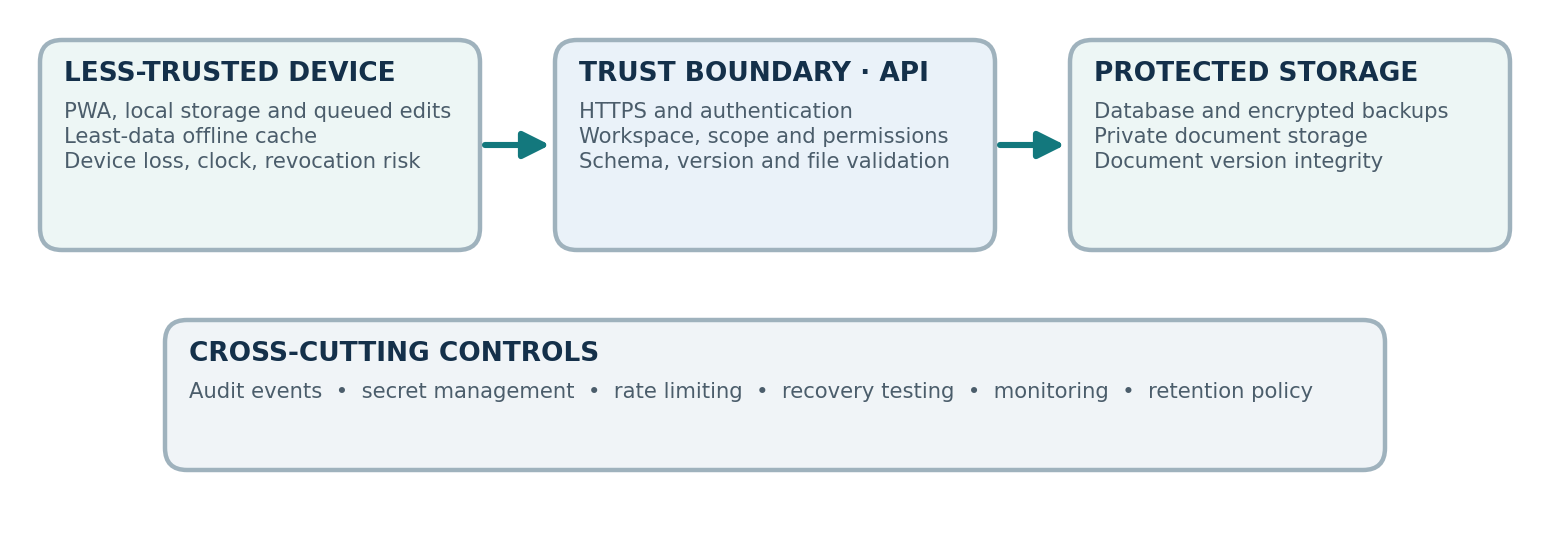
\includegraphics[width=\linewidth]{nfr-security-boundaries.png}
\caption{Proposed security boundaries and cross-cutting controls, adapted from the team's NFR contribution.}
\label{fig:nfr-security-boundaries}
\end{figure}

\Needspace{7\baselineskip}
\nfrheading{\identifier{SEC-01} --- Account authentication and password protection}\label{nfr:SEC-01}
The backend shall authenticate every application account using a unique, verified email identity and a password.

\textit{Rationale:} Protects the owner and included manager accounts against account takeover and enumeration.

\textit{Related:} \hyperref[fr:001]{\identifier{FR-001}}, \hyperref[fr:002]{\identifier{FR-002}}, \hyperref[fr:005]{\identifier{FR-005}}, \hyperref[fr:064]{\identifier{FR-064}}.
\begin{enumerate}[label=(\alph*),leftmargin=*,itemsep=1pt,topsep=3pt]
\item Only accounts with a verified email can access a business workspace; unverified accounts are refused.
\item Application-managed authentication uses established backend libraries and salted Argon2id password hashes; benchmark and record concrete cost parameters before deployment. Plaintext passwords are never stored or logged. A managed identity service is not the selected baseline.
\item Enforce at least 15 characters in the password-only flow and accept passphrases of at least 64 characters without silent truncation. Reject common/compromised passwords on registration, reset and change.
\item After five failed logins within 15 minutes, apply progressive throttling using account/source signals, without permanent attacker-triggered account lockout. Exact delay progression and recovery configuration require implementation review and tests.
\item Authentication failure responses do not disclose whether an email address is registered.
\end{enumerate}

\Needspace{7\baselineskip}
\nfrheading{\identifier{SEC-02} --- Online session lifecycle}\label{nfr:SEC-02}
Protected online requests shall use short-lived, revocable credentials.

\textit{Rationale:} Limits the exposure of stolen credentials and supports timely revocation.

\textit{Related:} \hyperref[fr:002]{\identifier{FR-002}}, \hyperref[fr:003]{\identifier{FR-003}}, \hyperref[fr:004]{\identifier{FR-004}}, \hyperref[fr:005]{\identifier{FR-005}}, \hyperref[fr:008]{\identifier{FR-008}}, \hyperref[fr:064]{\identifier{FR-064}}.
\begin{enumerate}[label=(\alph*),leftmargin=*,itemsep=1pt,topsep=3pt]
\item Online access credentials expire after 15 minutes; the server refuses expired credentials. Renewal is permitted only while the originating online session remains valid.
\item Renewable online sessions expire at most seven days after login, requiring authentication again; renewal does not extend that absolute limit. Implement revocation and rotation/replay protection. Cookie-based credentials use Secure, HttpOnly and an appropriate SameSite policy.
\item Logout revokes the applicable online session. Successful password reset or change invalidates existing online sessions. Membership revocation immediately denies that business online without deleting unrelated memberships.
\item An expired online session requires online renewal or authentication under its policy. It does not delete pending work or change the separate 15-day offline grant in \hyperref[nfr:AOC-02]{\identifier{AOC-02}}.
\end{enumerate}

\Needspace{7\baselineskip}
\nfrheading{\identifier{SEC-03} --- Workspace and operation-level authorisation}\label{nfr:SEC-03}
The server shall check authorisation on every protected read, write, export and file operation.

\textit{Rationale:} Preserves business isolation and independently granted consultation, entry and correction rights.

\textit{Related:} \hyperref[fr:002]{\identifier{FR-002}}, \hyperref[fr:004]{\identifier{FR-004}}, \hyperref[fr:007]{\identifier{FR-007}}, \hyperref[fr:008]{\identifier{FR-008}}, \hyperref[fr:023]{\identifier{FR-023}}, \hyperref[fr:038]{\identifier{FR-038}}, \hyperref[fr:053]{\identifier{FR-053}}; \hyperref[br:024]{\identifier{BR-024}}.
\begin{enumerate}[label=(\alph*),leftmargin=*,itemsep=1pt,topsep=3pt]
\item Each request validates account status and endpoint-specific authority. Technical provisioning requires the administrator system role; business operations require active workspace membership, responsibility scope and operation-specific grants. Administrator status alone grants no business-data/file authority.
\item A user-supplied identifier never establishes authority by itself.
\item Distinguish consultation, planning, entry, corrections, document association/modification, signing initiation and financial grants. Apply the included Field Manager defaults and mandatory scoped insurance access in Section~\ref{sec:permission-defaults}.
\item Supported financial actions may operate offline with the corresponding grants and prepared context; central acceptance revalidates them. Consultation/full-ticket access is disabled initially and requires an explicit owner grant within assigned scope; structured financial writes require additional grants.
\item Denied requests return a generic response that contains no protected data.
\end{enumerate}

\Needspace{7\baselineskip}
\nfrheading{\identifier{SEC-04} --- Encryption and private storage}\label{nfr:SEC-04}
Protected business data shall be encrypted in transit and in central storage; service credentials shall be protected and stored files private by default. Password storage follows \identifier{SEC-01} rather than reversible password encryption.

\textit{Rationale:} Protects employment, insurance and signing information across the device, API and storage boundaries.

\textit{Related:} \hyperref[fr:002]{\identifier{FR-002}}, \hyperref[fr:038]{\identifier{FR-038}}, \hyperref[fr:039]{\identifier{FR-039}}, \hyperref[fr:040]{\identifier{FR-040}}, \hyperref[fr:042]{\identifier{FR-042}}.
\begin{enumerate}[label=(\alph*),leftmargin=*,itemsep=1pt,topsep=3pt]
\item Production requests use HTTPS and a reviewed TLS/HSTS configuration. Plain HTTP is redirected or refused before protected content or credentials are served. The minimum supported protocol and deployment settings are reviewed under \decisionref{Q-TECH-01}.
\item Encrypt the central database, backups and private file storage at rest, with controlled key access and rotation. The hosting/key-management implementation is selected and verified during architecture review; this does not settle local-device protection under \decisionref{Q-DOC-07}.
\item Document storage is private by default; protected files are served only after API authorisation, using short-lived scoped retrieval links where applicable.
\item The central database is not directly reachable from the public internet.
\end{enumerate}

\Needspace{7\baselineskip}
\nfrheading{\identifier{SEC-05} --- Secure API, PWA and file validation}\label{nfr:SEC-05}
The backend shall validate every input and uploaded file independently of the PWA.

\textit{Rationale:} Prevents malicious requests, script injection and unsafe file handling; client-side validation does not replace server-side validation.

\textit{Related:} \hyperref[fr:001]{\identifier{FR-001}}, \hyperref[fr:038]{\identifier{FR-038}}, \hyperref[fr:040]{\identifier{FR-040}}, \hyperref[fr:045]{\identifier{FR-045}}, \hyperref[fr:049]{\identifier{FR-049}}, \hyperref[fr:051]{\identifier{FR-051}}, \hyperref[fr:053]{\identifier{FR-053}}, \hyperref[fr:063]{\identifier{FR-063}}, \hyperref[fr:064]{\identifier{FR-064}}.
\begin{enumerate}[label=(\alph*),leftmargin=*,itemsep=1pt,topsep=3pt]
\item Types, identifiers, relationships and file sizes are validated on the server, including references across business workspaces.
\item Use parameterised database access, context-appropriate output encoding, restrictive CORS and a deployable Content Security Policy. Cookie-authenticated state changes also require effective CSRF protection; CORS alone is not an authorisation or CSRF control.
\item Worker uploads accept PDF, JPG and PNG within the 10~MB (10,000,000-byte) per-file limit in \hyperref[br:044]{\identifier{BR-044}}. Validate content, size and safe file handling server-side, not only the extension. The team tests the 10,000,000-byte boundary and representative files under \decisionref{Q-DOC-06}; JPEG is accepted as the JPG image format.
\item Ticket, analysis and valuation evidence uses the same approved formats and 10~MB limit. Complete source files may be prepared offline with their consultation grants; monetary content neither forces classification/redaction nor prohibits upload under the applicable entry grant. Successful attachment replacement deletes its old file without history under \decisionref{Q-AT-02}; failed transfers preserve the old file and remain recoverable.
\item Scan application and bundled dependencies for known vulnerabilities in the delivery pipeline, triage findings and record remediation or explicit risk acceptance before release. A successful scan is not a claim of absence of vulnerabilities.
\end{enumerate}

\Needspace{7\baselineskip}
\nfrheading{\identifier{SEC-06} --- Secrets and deployment identities}\label{nfr:SEC-06}
Production credentials shall be kept out of source control and PWA assets, and every pipeline and service shall use least-privilege identities.

\textit{Rationale:} Prevents compromise through repository leakage or excessive pipeline privileges.

\textit{Related:} \hyperref[fr:001]{\identifier{FR-001}}, \hyperref[fr:005]{\identifier{FR-005}}, \hyperref[fr:040]{\identifier{FR-040}}.
\begin{enumerate}[label=(\alph*),leftmargin=*,itemsep=1pt,topsep=3pt]
\item Do not commit production service credentials or bundle database/email/storage secrets into the PWA. Device-local protection material, if used, follows the separate reviewed design under \decisionref{Q-DOC-07}.
\item Runtime services and delivery-pipeline jobs use separate identities with least privilege.
\item Keep production secrets in an access-controlled secrets mechanism with documented rotation and access review. Provider/tool selection remains an implementation decision.
\end{enumerate}

\Needspace{7\baselineskip}
\nfrheading{\identifier{SEC-07} --- Security-event audit logging}\label{nfr:SEC-07}
The server shall record security-relevant events.

\textit{Rationale:} Supports investigation and accountability while preserving the rule that ordinary business updates retain current values only (Section~\ref{sec:identity-current-values}).

\textit{Related:} \hyperref[fr:003]{\identifier{FR-003}}, \hyperref[fr:005]{\identifier{FR-005}}, \hyperref[fr:007]{\identifier{FR-007}}, \hyperref[fr:008]{\identifier{FR-008}}, \hyperref[fr:036]{\identifier{FR-036}}, \hyperref[fr:037]{\identifier{FR-037}}, \hyperref[fr:042]{\identifier{FR-042}}.
\begin{enumerate}[label=(\alph*),leftmargin=*,itemsep=1pt,topsep=3pt]
\item Each event records server timestamp, initiating account when known, workspace where applicable, action, minimal target identifier and outcome.
\item Mandatory server-observable categories: successful/failed authentication, logout, account recovery, membership and permission changes, restricted-document access requests handled by the API or controlled file service, signing acceptance, denied operations, revoked-access recovery decisions and security-relevant synchronisation conflicts. For document access, record the authorised retrieval/link-issuance decision or refusal; this does not prove that the user viewed the file.
\item Logs exclude passwords, raw tokens/full lifecycle links, document bodies, signature images, full official identification and raw monetary values; use minimal authorised identifiers.
\item Retain security events for 90 days from the server event, accessible only to authorised operations/investigation personnel. Purge thereafter, except justified incident preservation with a documented purpose and scope; test the configured schedule.
\item This requirement does not impose a permanent field-by-field history on ordinary corrections.
\item Opening a prepared file entirely offline is not logged in this version. Server preparation/retrieval/link issuance does not prove viewing. This coverage choice does not weaken file-access authorisation.
\end{enumerate}

\Needspace{7\baselineskip}
\nfrheading{\identifier{SEC-08} --- Document and signature integrity}\label{nfr:SEC-08}
Each accepted document version and each confirmed signature shall be tamper-evident and bound to the exact version signed.

\textit{Rationale:} Preserves integrity and provenance while respecting current-source replacement policy and withdrawal.

\textit{Related:} \hyperref[fr:038]{\identifier{FR-038}}, \hyperref[fr:041]{\identifier{FR-041}}, \hyperref[fr:042]{\identifier{FR-042}}, \hyperref[fr:043]{\identifier{FR-043}}, \hyperref[fr:044]{\identifier{FR-044}}, \hyperref[fr:045]{\identifier{FR-045}}; \hyperref[br:026]{\identifier{BR-026}}.
\begin{enumerate}[label=(\alph*),leftmargin=*,itemsep=1pt,topsep=3pt]
\item Each current accepted source has an immutable file identity and protected cryptographic digest. Verify source bytes against that digest. Validate the rendition against its own source/worker/signature associations; a derived PDF is not compared with the source digest. The team selects/tests the digest algorithm and metadata protection; a hash is not signer identification.
\item Bind a confirmed drawing to its worker, authorised initiator, exact source and confirmation time.
\item Never transfer a drawing or choice to another source/worker or overwrite signed bytes in place. A replacement needs its own worker review/signing.
\item Apply \identifier{BR-026}: only after successful replacement, delete the superseded source, signature and PDF, including signed contracts/externally declared signed uploads. Invalidate old-source signing and propagate received deletion to prepared copies. Temporary rejected-proposal recovery follows \decisionref{Q-DOC-04}, without a history browser.
\item Record server acceptance time separately from device confirmation time.
\item A drawn mark alone is not represented as a qualified electronic signature.
\end{enumerate}

\Needspace{7\baselineskip}
\nfrheading{\identifier{SEC-09} --- Verification, recovery and invitation tokens}\label{nfr:SEC-09}
Account-lifecycle links shall be single-use, short-lived and unpredictable.

\textit{Rationale:} Protects registration, recovery and invitation flows from replay, enumeration and unauthorised business membership.

\textit{Related:} \hyperref[fr:001]{\identifier{FR-001}}, \hyperref[fr:005]{\identifier{FR-005}}, \hyperref[fr:006]{\identifier{FR-006}}, \hyperref[fr:064]{\identifier{FR-064}}.
\begin{enumerate}[label=(\alph*),leftmargin=*,itemsep=1pt,topsep=3pt]
\item Owner-activation and email-verification links, including replacement-email verification, expire after 24 hours and are single-use. An unverified replacement cannot supersede the active email; a resend invalidates the preceding link.
\item Password-reset links expire after 30 minutes and are single-use. Resending invalidates the preceding link; invalid/expired/consumed links cannot change credentials.
\item Invitations expire after seven days and are single-use, bound to the intended verified email and business. Resending/cancelling invalidates superseded links without duplicate membership.
\item Generate token values unpredictably and store only a verification hash or equivalent protected verifier when persisted. Consume/invalidate lifecycle authorisations transactionally. Retries may report an already completed action without repeating activation, membership creation or credential changes.
\item A successful reset revokes existing online sessions without changing business ownership.
\end{enumerate}

\Needspace{7\baselineskip}
\nfrheading{\identifier{SEC-10} --- Abuse protection and rate limiting}\label{nfr:SEC-10}
The API shall limit request rates to protect availability and prevent automated abuse.

\textit{Rationale:} \hyperref[nfr:SEC-01]{\identifier{SEC-01}} throttles login attempts only; recovery, invitation, upload and email-triggering endpoints can also be abused.

\textit{Related:} \hyperref[fr:001]{\identifier{FR-001}}, \hyperref[fr:005]{\identifier{FR-005}}, \hyperref[fr:006]{\identifier{FR-006}}, \hyperref[fr:040]{\identifier{FR-040}}.
\begin{enumerate}[label=(\alph*),leftmargin=*,itemsep=1pt,topsep=3pt]
\item Use account/source/recipient-aware limits as applicable: unauthenticated operations cannot depend on an authenticated account key. Apply stricter reviewed controls to authentication, recovery, invitations, uploads and email-triggering requests.
\item Exceeded limits return a generic, retryable rejection and do not affect other accounts.
\item Resending verification, reset and invitation messages is limited per recipient address.
\item The approved login threshold is five failures within 15 minutes under SEC-01. Endpoint-specific recovery, resend, upload and invitation limits and progressive delays still require configuration review; verify recipient/account isolation before release.
\end{enumerate}

\Needspace{7\baselineskip}
\nfrheading{\identifier{SEC-11} --- Email delivery security}\label{nfr:SEC-11}
Verification, recovery and invitation messages shall be sent through an authenticated and monitored email delivery service.

\textit{Rationale:} Protects account activation, recovery, verified-email changes and invitations that depend on email delivery.

\textit{Related:} \hyperref[fr:001]{\identifier{FR-001}}, \hyperref[fr:005]{\identifier{FR-005}}, \hyperref[fr:006]{\identifier{FR-006}}, \hyperref[fr:064]{\identifier{FR-064}}.
\begin{enumerate}[label=(\alph*),leftmargin=*,itemsep=1pt,topsep=3pt]
\item The sending domain is authenticated with SPF, DKIM and DMARC.
\item Messages contain the intended lifecycle link and minimal account context, never passwords, worker data or protected documents.
\item A send failure preserves the pending account/invitation state without duplicate identities or memberships. Offer rate-limited resend, invalidating the preceding lifecycle link. Recovery acknowledgements remain generic regardless of registration status.
\item Record the provider, its processing role/terms, sending-domain configuration and any transfers in the processing inventory under \hyperref[nfr:PRV-05]{\identifier{PRV-05}}; provider selection remains under \decisionref{Q-NFR-05}.
\end{enumerate}

\paragraph{Email delivery operation.}
Only the backend calls the transactional email service using protected credentials.
Record technical send outcomes and provider failures without full links. Provider
acceptance does not prove inbox delivery or reading. Development/demo sending uses
controlled recipients or a test environment. Provider, authorised sender domain and
concrete configuration remain under \decisionref{Q-NFR-05}.

\paragraph{Technical references.}
Password and session controls are informed by the
\href{https://cheatsheetseries.owasp.org/cheatsheets/Authentication_Cheat_Sheet.html}{OWASP Authentication},
\href{https://cheatsheetseries.owasp.org/cheatsheets/Password_Storage_Cheat_Sheet.html}{Password Storage}
and \href{https://cheatsheetseries.owasp.org/cheatsheets/Session_Management_Cheat_Sheet.html}{Session Management}
guidance. These references do not approve project-specific numeric targets.

\paragraph{Administrator provisioning verification.}
Check administrator-only owner setup, single-client concurrency/idempotency,
expired/replayed activation, controlled resend and recipient-chosen password.
Unauthenticated users, owners and managers cannot call technical provisioning;
technical administrators cannot read agricultural records/files by system role alone.
Manager signup requires an intended valid owner invitation. Bootstrap credentials
are deployment-managed; passwords never enter provisioning messages or logs.

\subsection{Privacy}
\label{sec:nfr-privacy}
Protect account data and worker records, including required official identification,
insurance, employment documents, drawn signatures and examination-consent choices.
Clinical findings are outside this form workflow. Source member references and
official worker identifiers remain protected business data. The processing basis and
retention duties must be validated for the actual context; technical controls alone
do not establish GDPR compliance. \identifier{PRV-04} defines governance procedures without
silently adding account deletion or worker self-service to the functional scope.

\Needspace{7\baselineskip}
\nfrheading{\identifier{PRV-01} --- Personal-data minimisation and purpose limitation}\label{nfr:PRV-01}
The application shall collect and expose only the personal data needed for documented purposes.

\textit{Rationale:} Workers have no management accounts; owners and authorised managers process their records within a business workspace.

\textit{Related:} \hyperref[fr:020]{\identifier{FR-020}} to \hyperref[fr:023]{\identifier{FR-023}}, \hyperref[fr:038]{\identifier{FR-038}}, \hyperref[fr:039]{\identifier{FR-039}}, \hyperref[fr:053]{\identifier{FR-053}}.
\begin{enumerate}[label=(\alph*),leftmargin=*,itemsep=1pt,topsep=3pt]
\item Document the purpose and necessity of account/worker attributes, including the official type, country and number required by \hyperref[fr:020]{\identifier{FR-020}}. Required entry does not itself establish a lawful basis or require collection of a scanned copy.
\item Each cached dataset and exported report is limited to the authenticated user's authorised responsibilities.
\item Full document contents and unrelated personal identifiers are not copied into dashboards or technical logs.
\end{enumerate}

\Needspace{7\baselineskip}
\nfrheading{\identifier{PRV-02} --- Lawful processing and transparency}\label{nfr:PRV-02}
The responsible business shall document the lawful basis for worker data before real data are processed.

\textit{Rationale:} Consent may be inappropriate or insufficient in an employment relationship; compliance depends on purpose and legal context, not on hosting location.

\textit{Related:} \hyperref[fr:020]{\identifier{FR-020}} to \hyperref[fr:023]{\identifier{FR-023}}, \hyperref[fr:038]{\identifier{FR-038}} to \hyperref[fr:045]{\identifier{FR-045}}.
\begin{enumerate}[label=(\alph*),leftmargin=*,itemsep=1pt,topsep=3pt]
\item Before real worker data are used, the purposes, applicable lawful bases, privacy notice and processor responsibilities are documented for worker records, insurance, employment documents and signatures.
\item Do not assume that a generic GDPR consent signature authorises all employment processing. Validate the applicable basis by purpose, including any sensitive information in supplied documents; unresolved questions remain under \decisionref{Q-NFR-03}.
\item Academic demonstration and test environments use synthetic or appropriately anonymised data unless real-data processing has been authorised.
\end{enumerate}

\Needspace{7\baselineskip}
\nfrheading{\identifier{PRV-03} --- Protected local data and account isolation}\label{nfr:PRV-03}
Data held on the device shall be limited, isolated by account and protected after logout or revocation.

\textit{Rationale:} Prepared insurance and signing documents must be available offline while unsent work is safeguarded on logout.

\textit{Related:} \hyperref[fr:003]{\identifier{FR-003}}, \hyperref[fr:004]{\identifier{FR-004}}, \hyperref[fr:008]{\identifier{FR-008}}, \hyperref[fr:039]{\identifier{FR-039}}, \hyperref[fr:045]{\identifier{FR-045}}.
\begin{enumerate}[label=(\alph*),leftmargin=*,itemsep=1pt,topsep=3pt]
\item Prepared local datasets contain only authorised required context, with pending local records/dependencies created through supported offline operations stored separately from the accepted baseline.
\item Private data and pending operations are logically isolated by originating account and business workspace.
\item Logout immediately blocks workspace access and isolates retained information. Disposable accepted copies may be removed under the local policy; the 30-day inactivity cleanup in \hyperref[fr:003]{\identifier{FR-003}} removes only eligible accepted copies and never pending recovery dependencies.
\item Normal recovery requires the originating account and renewed authority. The separate revoked-manager owner-review procedure in \hyperref[fr:008]{\identifier{FR-008}}/\hyperref[nfr:REL-08]{\identifier{REL-08}} preserves original authorship without restoring normal access or exposing pending work to another account.
\item On reconnection, refresh authority before normal protected access/acceptance and apply authorised access/deletion changes. Preserve quarantined pending proposals and required recovery files under the separate recovery policy.
\item The system does not claim that a disconnected device can be remotely wiped immediately.
\item Encrypt device-held personal data, protected files and pending operations, isolated by origin account and business. Logout locks protected access while preserving recovery dependencies. Another account cannot read or submit them. Concrete encryption/key lifecycle and trusted-time mechanisms require a technical proof under \decisionref{Q-DOC-07}; browser-origin isolation or screen lock alone is insufficient.
\end{enumerate}

\Needspace{7\baselineskip}
\nfrheading{\identifier{PRV-04} --- Rights, retention and permitted erasure}\label{nfr:PRV-04}
Personal-data requests shall follow a documented authorised procedure that respects applicable rights, dependencies and validated retention duties.

\textit{Rationale:} Distinguishes rights handling from ordinary record deletion and avoids inventing unapproved self-service workflows.

\textit{Related:} \hyperref[fr:003]{\identifier{FR-003}}, \hyperref[fr:021]{\identifier{FR-021}} to \hyperref[fr:023]{\identifier{FR-023}}, \hyperref[fr:038]{\identifier{FR-038}}, \hyperref[fr:041]{\identifier{FR-041}}; \hyperref[br:026]{\identifier{BR-026}}.
\begin{enumerate}[label=(\alph*),leftmargin=*,itemsep=1pt,topsep=3pt]
\item Handle consultation, correction and erasure requests manually: the owner receives/follows the request; a designated technical responsible person intervenes when necessary and authorised. No dedicated request-management portal is included.
\item Record request identity, scope, authorisation, action and response through a controlled procedure. Assess dependencies and applicable processing duties; archival/inactivation is not itself erasure.
\item While a source exists, its contents and signing evidence remain immutable. Successful replacement deletes the previous source, signature and PDF for every category under \identifier{BR-026}, with no inherited signature or consultable history. A failed upload preserves the current source.
\item The agreed product rule keeps current documents until replacement rather than assigning an invented fixed number of years. Document the applicable purposes/notices and operating responsibilities before real-data use; deployment review does not assert completed legal validation.
\item Backup expiry and restore suppression follow \identifier{REL-04}. Apply retained deletion decisions before restoring normal access; do not claim immediate erasure from every backup or disconnected device.
\item Controlled account/data requests follow this manual procedure under \decisionref{Q-AA-07}; owner-facing business closure is excluded under \decisionref{Q-SCOPE-07}. Verified email changes under \identifier{FR-064} preserve account identity.
\end{enumerate}

\Needspace{7\baselineskip}
\nfrheading{\identifier{PRV-05} --- Processing location and breach response}\label{nfr:PRV-05}
Processing locations, providers and transfers shall be reviewed, and an operational personal-data incident procedure shall exist.

\textit{Rationale:} Hosting location alone does not establish GDPR compliance; organisational responsibilities and transfer arrangements also matter.

\textit{Related:} \hyperref[fr:001]{\identifier{FR-001}} to \hyperref[fr:008]{\identifier{FR-008}}, \hyperref[fr:038]{\identifier{FR-038}} to \hyperref[fr:045]{\identifier{FR-045}}.
\begin{enumerate}[label=(\alph*),leftmargin=*,itemsep=1pt,topsep=3pt]
\item Approve primary, backup, telemetry and support-processing locations before real-data deployment. EU-region hosting is the submitted preference for review under \decisionref{Q-NFR-03}, not a settled provider/deployment decision or a substitute for transfer assessment.
\item Processing terms and any international transfers are verified for infrastructure, support, telemetry and email-delivery providers.
\item An incident-response procedure identifies the controller contact, escalation route, containment and assessment steps.
\item Where GDPR Article 33 applies, the controller assesses notification without undue delay and, where feasible, within 72 hours after awareness, unless the breach is unlikely to risk individuals' rights and freedoms. Record the assessment and any reasons for delay; applicability and responsibility are validated under \decisionref{Q-NFR-03}.
\end{enumerate}

\Needspace{7\baselineskip}
\nfrheading{\identifier{PRV-06} --- Privacy-preserving telemetry}\label{nfr:PRV-06}
Logs, analytics and diagnostics shall not become an uncontrolled second copy of personal or financial data.

\textit{Rationale:} Observability must not expose protected documents or monetary values.

\textit{Related:} \hyperref[fr:038]{\identifier{FR-038}}, \hyperref[fr:045]{\identifier{FR-045}}, \hyperref[fr:053]{\identifier{FR-053}} to \hyperref[fr:062]{\identifier{FR-062}}.
\begin{enumerate}[label=(\alph*),leftmargin=*,itemsep=1pt,topsep=3pt]
\item Logs, analytics, error reports, queue diagnostics and deployment artefacts minimise personal data and exclude full official identification, document bodies and captured drawings. Operational identifiers are limited to the authorised diagnostic purpose.
\item Diagnostic records use record identifiers and minimal contextual metadata, with access control and a retention schedule.
\item Do not copy monetary values or protected document contents into technical diagnostics. This does not prohibit authorised financial business data, prepared offline consultation or PDF indicators under \hyperref[fr:053]{\identifier{FR-053}}, \hyperref[fr:060]{\identifier{FR-060}} and \hyperref[fr:062]{\identifier{FR-062}}.
\end{enumerate}

\Needspace{7\baselineskip}
\nfrheading{\identifier{PRV-07} --- Offline document retention and deletion propagation}\label{nfr:PRV-07}
Offline document preparation shall be selective, and deletions made centrally shall reach local copies.

\textit{Rationale:} Offline insurance and signing (\hyperref[fr:039]{\identifier{FR-039}}, \hyperref[fr:045]{\identifier{FR-045}}) must not expand personal-data exposure unnecessarily.

\textit{Related:} \hyperref[fr:038]{\identifier{FR-038}}, \hyperref[fr:039]{\identifier{FR-039}}, \hyperref[fr:041]{\identifier{FR-041}}, \hyperref[fr:042]{\identifier{FR-042}}, \hyperref[fr:045]{\identifier{FR-045}}.
\begin{enumerate}[label=(\alph*),leftmargin=*,itemsep=1pt,topsep=3pt]
\item Preparation covers current insurance versions for the prepared worker window and explicitly selected workers, and only specifically prepared versions for offline signing.
\item Contracts are never bulk-downloaded automatically.
\item Local file/reference metadata identifies the originating account and workspace, associated worker and version or authorised business target, access context and freshness and the document's single worker identity.
\item Apply received access, withdrawal and deletion changes to prepared copies. Remove superseded accepted source, signature and PDF copies after receiving replacement deletion; route ineligible pending signing to protected temporary recovery without resurrecting the old source. A withdrawn current source remains consultable until replacement but is ineligible for signing; replaced sources have no history view; exclusive local conflicts follow \decisionref{Q-DOC-04}.
\item Queued retries never recreate a deleted version.
\end{enumerate}

\paragraph{Regulatory reference.}
Validate the applicable duties against
\href{https://eur-lex.europa.eu/eli/reg/2016/679/oj}{Regulation (EU) 2016/679},
including purpose/minimisation, lawful basis, rights, processors, security,
notification and transfers. The incident-notification time in \identifier{PRV-05} is a conditional
legal requirement, not a proposed service-level target or a certification of compliance.

\subsection{Reliability and Recovery}
\label{sec:nfr-reliability}
These requirements protect accepted data and recoverable proposals during retries,
concurrent edits, interrupted transfers, upgrades and central recovery. The protocol
in Section~\ref{sec:offline-sync} supplies the interaction detail; the synchronisation
state definitions remain in Section~\ref{sec:sync-states}. Backup and service targets
are approved specification targets, not measured outcomes or provider guarantees.

\Needspace{7\baselineskip}
\nfrheading{\identifier{REL-01} --- Idempotent server processing}\label{nfr:REL-01}
Every mutating operation shall have the same business effect however many times it is submitted.

\textit{Rationale:} Retries after disconnection must not duplicate business records or signatures.

\textit{Related:} \hyperref[fr:001]{\identifier{FR-001}}, \hyperref[fr:003]{\identifier{FR-003}}, \hyperref[fr:006]{\identifier{FR-006}}, \hyperref[fr:029]{\identifier{FR-029}}, \hyperref[fr:041]{\identifier{FR-041}}, \hyperref[fr:043]{\identifier{FR-043}}, \hyperref[fr:048]{\identifier{FR-048}}.
\begin{enumerate}[label=(\alph*),leftmargin=*,itemsep=1pt,topsep=3pt]
\item Mutations carry stable operation\_id, origin, payload fingerprint and dependencies. Persist minimal outcomes for 90 days after processing. Identical retries have one effect; reused IDs with different content are refused. Expired-context submissions require reviewed recovery, never blind replay that could duplicate effects or recreate deleted records.
\item Creation of users, memberships, attendance, deliveries, document versions and signatures is protected against duplicate retries.
\item Related database changes and the idempotency outcome commit atomically. Transfers to object storage have a recoverable readiness/cleanup protocol; this is not a claim of one database/object-store transaction.
\end{enumerate}

\Needspace{7\baselineskip}
\nfrheading{\identifier{REL-02} --- Optimistic concurrency and conflict resolution}\label{nfr:REL-02}
Concurrent changes to shared records shall never be silently overwritten.

\textit{Rationale:} Supports informed user review of competing corrections.

\textit{Related:} \hyperref[fr:008]{\identifier{FR-008}}, \hyperref[fr:036]{\identifier{FR-036}}, \hyperref[fr:037]{\identifier{FR-037}}, \hyperref[fr:043]{\identifier{FR-043}}.
\begin{enumerate}[label=(\alph*),leftmargin=*,itemsep=1pt,topsep=3pt]
\item Every mutable shared record has a server-managed revision, and each update carries the client's base revision.
\item A version mismatch never overwrites accepted server state; the pending proposal is preserved.
\item The user sees accepted and proposed values side by side for authorised manual review.
\item Resubmission after review revalidates permissions, campaign state, dependencies and business rules.
\item Automatic last-write-wins is not used for any persisted business record.
\end{enumerate}

\Needspace{7\baselineskip}
\nfrheading{\identifier{REL-03} --- Cross-entity integrity and consistent calculations}\label{nfr:REL-03}
The API and the database shall enforce integrity rules, and server-side validation shall be authoritative even for data entered offline.

\textit{Rationale:} Ensures dashboard correctness and prevents cross-workspace or cross-campaign corruption.

\textit{Related:} \hyperref[fr:026]{\identifier{FR-026}} to \hyperref[fr:037]{\identifier{FR-037}}, \hyperref[fr:046]{\identifier{FR-046}} to \hyperref[fr:062]{\identifier{FR-062}}.
\begin{enumerate}[label=(\alph*),leftmargin=*,itemsep=1pt,topsep=3pt]
\item Foreign-key, uniqueness, business-scope and status-transition constraints are enforced.
\item Actual work periods are not double counted across assignments, campaigns or adjacent dates.
\item Delivery-based totals require Delivered, non-cancelled parents under \hyperref[br:038]{\identifier{BR-038}}. Pre-arrival source data awaits receipt confirmation. Ticket deductions are not applied twice; missing analyses are not treated as zero.
\item For one ticket, replacing a provisional amount with final retains one current valuation, never additive revisions. Separate provisional/final totals across different eligible tickets remain valid and do not imply payments.
\item Server-side validation prevails over local validation for data that originated offline.
\end{enumerate}

\Needspace{7\baselineskip}
\nfrheading{\identifier{REL-04} --- Central backup and tested recovery}\label{nfr:REL-04}
Central data shall be backed up and recoverable within stated targets.
The recovery point objective (RPO) bounds the recoverable data-loss window;
the recovery time objective (RTO) bounds the time to restore the agreed service
after a declared incident. Record both measurement boundaries in the rehearsal.

\textit{Rationale:} Makes central persistence recoverable; measurable objectives depend on an agreed deployment and a rehearsed restore procedure.

\textit{Related:} \hyperref[fr:003]{\identifier{FR-003}}, \hyperref[fr:038]{\identifier{FR-038}} to \hyperref[fr:045]{\identifier{FR-045}}, \hyperref[fr:046]{\identifier{FR-046}} to \hyperref[fr:062]{\identifier{FR-062}}; \hyperref[br:026]{\identifier{BR-026}}.
\begin{enumerate}[label=(\alph*),leftmargin=*,itemsep=1pt,topsep=3pt]
\item Automate encrypted central database and compatible file/evidence backups at least daily. Preserve database/file dependencies together, restrict access and alert on failed scheduled backups.
\item Retain central backups for at least 14 days. This is a recovery policy, not an employment or signed-document retention period or proof of immediate erasure from all backups.
\item Rehearse RPO at most 24 hours and RTO at most four hours against the agreed deployment/data restore scope. The accepted RPO permits up to 24 hours of central-data loss. These targets do not recover unsent records on a lost device.
\item Before restoring ordinary service, reapply retained authorised deletion/restriction and access decisions that postdate the backup. Retain recovery metadata independently long enough to enforce them; if it is insufficient, quarantine affected data rather than exposing erased/restricted records.
\item At least one representative restore rehearsal is performed before operational deployment, validating relationships and accessible retained document versions.
\end{enumerate}

\Needspace{7\baselineskip}
\nfrheading{\identifier{REL-05} --- Monitoring and incident response}\label{nfr:REL-05}
Failures shall be detected and reach a named team contact during the harvest period.

\textit{Rationale:} Field work may continue locally during cloud incidents, but failures must be detected for recovery and eventual synchronisation.

\textit{Related:} \hyperref[fr:004]{\identifier{FR-004}}, \hyperref[fr:037]{\identifier{FR-037}}, \hyperref[fr:043]{\identifier{FR-043}}, \hyperref[fr:048]{\identifier{FR-048}}.
\begin{enumerate}[label=(\alph*),leftmargin=*,itemsep=1pt,topsep=3pt]
\item Monitoring covers API reachability, elevated error rates, failed scheduled backups, storage capacity and abnormal synchronisation failures.
\item Alerts reach an assigned operational contact under a documented response arrangement and produce an incident record. The response coverage and thresholds must be agreed; no unapproved round-the-clock service guarantee is implied.
\item Monitoring complies with \hyperref[nfr:PRV-06]{\identifier{PRV-06}}.
\end{enumerate}

\Needspace{7\baselineskip}
\nfrheading{\identifier{REL-06} --- Validated deployments and rollback}\label{nfr:REL-06}
Releases shall be tested, reversible and safe for devices holding queued work.

\textit{Rationale:} Protects campaign continuity from software releases made while clients are disconnected.

\textit{Related:} \hyperref[fr:003]{\identifier{FR-003}}, \hyperref[fr:004]{\identifier{FR-004}}, \hyperref[fr:037]{\identifier{FR-037}}, \hyperref[fr:045]{\identifier{FR-045}}.
\begin{enumerate}[label=(\alph*),leftmargin=*,itemsep=1pt,topsep=3pt]
\item Changes pass automated tests and schema-compatibility checks in a staging environment before release.
\item A deployable previous version and a documented rollback procedure, including migration compatibility, are preserved.
\item A release never discards locally queued changes or requires a destructive upgrade.
\item Staging and test environments use synthetic or appropriately anonymised data (\hyperref[nfr:PRV-02]{\identifier{PRV-02}}).
\end{enumerate}

\Needspace{7\baselineskip}
\nfrheading{\identifier{REL-07} --- Older PWA client compatibility}\label{nfr:REL-07}
Devices running an earlier PWA release shall still be able to synchronise or be told how to recover.

\textit{Rationale:} Prepared clients may run old releases; an expired offline grant still leaves pending data requiring safe recovery.

\textit{Related:} \hyperref[fr:003]{\identifier{FR-003}}, \hyperref[fr:004]{\identifier{FR-004}}, \hyperref[fr:037]{\identifier{FR-037}}, \hyperref[fr:043]{\identifier{FR-043}}.
\begin{enumerate}[label=(\alph*),leftmargin=*,itemsep=1pt,topsep=3pt]
\item Support the immediately preceding client release and required payload formats for 30 days after a new release. Preserve queued records/files from unsupported or stale contexts for reviewed recovery; refresh prepared data without blind replay. The server-issued context, not device time alone, establishes eligibility.
\item Schema transformations never silently discard fields or reinterpret identifiers.
\end{enumerate}

\Needspace{7\baselineskip}
\nfrheading{\identifier{REL-08} --- Revoked-access and rejected-operation recovery}\label{nfr:REL-08}
Pending operations associated with a revoked business membership, and rejected
operations, shall remain protected and recoverable under the applicable review
procedure. Revoking membership does not revoke the account in other businesses.

\textit{Rationale:} Implements the \hyperref[fr:008]{\identifier{FR-008}} recovery flow and offline signing safety.

\textit{Related:} \hyperref[fr:003]{\identifier{FR-003}}, \hyperref[fr:004]{\identifier{FR-004}}, \hyperref[fr:008]{\identifier{FR-008}}, \hyperref[fr:037]{\identifier{FR-037}}, \hyperref[fr:041]{\identifier{FR-041}}, \hyperref[fr:043]{\identifier{FR-043}}, \hyperref[fr:045]{\identifier{FR-045}}.
\begin{enumerate}[label=(\alph*),leftmargin=*,itemsep=1pt,topsep=3pt]
\item Revoking a manager membership immediately denies normal online actions in that business. Disconnected enforcement follows \hyperref[br:002]{\identifier{BR-002}} and \hyperref[nfr:AOC-02]{\identifier{AOC-02}}; the manager role is included.
\item After origin-account authentication, allow restricted recovery submission without normal business read/write access. The owner accepts or rejects each proposal. Acceptance is new explicit authorisation, subject to normal lifecycle, date, coverage, revision, dependency and integrity checks. Client timestamps do not prove pre-revocation creation; automatic distinction from fabricated prior work is not promised. Concrete protected transport/quarantine/expiry remain implementation validation tasks.
\item The originating account and the accepting owner are recorded as distinct in the recovery event.
\item Rejected/conflicting/uncertain outcomes remain distinct and recoverable. A replacement deletes the superseded source; pending signing against it is rejected and cannot be transferred or resurrected. Withdrawn/deleted sources permit inspection/rejection with a reason, not owner-authorised signature validity or automatic resurrection. A valid current source needs fresh worker review and signing. The team defines/tests protected temporary recovery and cleanup within the no-history policy.
\end{enumerate}

\paragraph{Synchronisation metadata lifetime.}
Retain authorised change-feed/deletion markers for 90 days. Beyond the supported
window, require a scoped refresh and reviewed recovery of older proposals; never
infer that a missing operation outcome means an unprocessed operation. Validate
server-context expiry and anti-resurrection safeguards in the technical slice.
These metadata are not a permanent business correction history and do not replace
security-event or document retention.

\subsection{Availability and Offline Continuity}
\label{sec:nfr-offline}
Offline continuity is operation-specific and follows \hyperref[br:013]{\identifier{BR-013}}.
Online availability and prepared field use are separate properties. The 15-day
authorisation already agreed in \decisionref{D-22} remains unchanged; additional
approved availability/performance targets are coordinated through \decisionref{Q-NFR-02}
and \decisionref{Q-NFR-07}.
\paragraph{Simple routine interaction.}\label{sec:offline-interaction}
Use the ordinary field forms, clear locally-saved/pending status and automatic sync
attempts with a manual retry when connected. Do not require routine outbox management.
Genuine conflicts or changed grants need an explicit recoverable exception workflow.
The demonstration's simplified interface does not establish production persistence,
authorisation enforcement or recovery.

\Needspace{7\baselineskip}
\nfrheading{\identifier{AOC-01} --- Prepared offline operational continuity}\label{nfr:AOC-01}
After online authentication and preparation, the PWA shall support the operations that the use cases designate as available offline.

\textit{Rationale:} Maintains field continuity with the same forms and operation-specific grants rather than an unrestricted offline application.

\textit{Related:} \hyperref[fr:004]{\identifier{FR-004}}, \hyperref[fr:011]{\identifier{FR-011}}, \hyperref[fr:015]{\identifier{FR-015}}, \hyperref[fr:016]{\identifier{FR-016}}, \hyperref[fr:020]{\identifier{FR-020}}, \hyperref[fr:023]{\identifier{FR-023}}, \hyperref[fr:028]{\identifier{FR-028}}, \hyperref[fr:029]{\identifier{FR-029}}, \hyperref[fr:034]{\identifier{FR-034}}, \hyperref[fr:037]{\identifier{FR-037}}, \hyperref[fr:039]{\identifier{FR-039}}, \hyperref[fr:045]{\identifier{FR-045}}, \hyperref[fr:048]{\identifier{FR-048}}--\hyperref[fr:054]{\identifier{FR-054}}, \hyperref[fr:060]{\identifier{FR-060}}, \hyperref[fr:062]{\identifier{FR-062}}.
\begin{enumerate}[label=(\alph*),leftmargin=*,itemsep=1pt,topsep=3pt]
\item Support prepared consultation, optional planning, attendance/work and authorised corrections, deliveries/results, selected-version signing and financial consultation, entry, correction and PDF output under their FR grants. Explicit campaign start and identified same-day worker creation also work offline with stable pending dependencies.
\item Initial authentication, account/access administration, property/parcel structure, campaign creation/coverage/closure/reopening, existing-worker administration, source-version management and template generation require connectivity. Do not confuse these with the supported worker-create/campaign-start exceptions.
\item Offline operation is not presented as access to all historical data; unavailable local data is distinguished from an empty result.
\item Prepared financial values, complete tickets and source files follow the financial/full-content grants in Section~\ref{sec:permission-defaults}. Do not exclude monetary data from offline views or require content classification/redaction. Structured records and file-transfer readiness remain separate.
\item Expose readiness for schedules in the current and following week and current insurance, including explicitly selected existing workers. Other permitted signing documents require explicit preparation; apply \hyperref[br:029]{\identifier{BR-029}} without automatically downloading all contracts.
\item Distinguish metadata and file readiness. Interrupted preparation, unavailable files and insufficient storage must not produce a false ready state; coordinate storage guidance with \hyperref[nfr:AOC-05]{\identifier{AOC-05}}.
\end{enumerate}

\Needspace{7\baselineskip}
\nfrheading{\identifier{AOC-02} --- Bounded offline authorisation}\label{nfr:AOC-02}
A device shall operate offline only for a limited time after its latest successful online permission validation.

\textit{Rationale:} Balances seasonal field connectivity against the risk of lost devices and delayed revocation.

\textit{Related:} \hyperref[fr:002]{\identifier{FR-002}}, \hyperref[fr:003]{\identifier{FR-003}}, \hyperref[fr:004]{\identifier{FR-004}}, \hyperref[fr:005]{\identifier{FR-005}}, \hyperref[fr:008]{\identifier{FR-008}}.
\begin{enumerate}[label=(\alph*),leftmargin=*,itemsep=1pt,topsep=3pt]
\item Prepared offline authorisation expires 15 days after the latest successful online validation of permissions, as already defined in \hyperref[fr:004]{\identifier{FR-004}} and \identifier{D-22}. Only another successful online validation renews it.
\item The 15-day grant is separate from online credential/session expiry, the current/following-week preparation window and the 30-day accepted-cache inactivity cleanup.
\item On expiry, protected offline access is locked until the device is revalidated online.
\item Expiry never deletes pending operations: they stay protected in the local queue and are submitted after revalidation, subject to server-side authorisation (including \hyperref[nfr:REL-08]{\identifier{REL-08}} for revoked managers).
\item Protect the validation/expiry context against clock rollback and fail closed when its trusted-time context cannot be established. Keeping server time or detecting rollback is a proposed safeguard, not proof against arbitrary clock manipulation; the final method and boundary tests remain under \decisionref{Q-DOC-07}.
\item Reconnection revalidates current access and permissions before any pending operation is accepted.
\end{enumerate}

\Needspace{7\baselineskip}
\nfrheading{\identifier{AOC-03} --- Persistent operation queue and visible states}\label{nfr:AOC-03}
Every offline change shall be stored durably, and its synchronisation state shall be visible.

\textit{Rationale:} Prevents a locally saved entry from being mistaken for a server-accepted record and makes connectivity failures recoverable.

\textit{Related:} \hyperref[fr:003]{\identifier{FR-003}}, \hyperref[fr:004]{\identifier{FR-004}}, \hyperref[fr:029]{\identifier{FR-029}}, \hyperref[fr:034]{\identifier{FR-034}}, \hyperref[fr:037]{\identifier{FR-037}}, \hyperref[fr:043]{\identifier{FR-043}}.
\begin{enumerate}[label=(\alph*),leftmargin=*,itemsep=1pt,topsep=3pt]
\item Persist the business proposal and outbox entry atomically before local confirmation, with stable record/operation identities, origin account/workspace, base revision, dependencies, payload and recorded time. File-transfer readiness is tracked separately.
\item After successful durable local saving, pending records and confirmed signing proposals survive normal PWA closure/reopening, temporary network loss and device restart while the supported browser storage remains intact. This does not guarantee survival after eviction, deliberate clearing or device loss.
\item Use the states in Section~\ref{sec:sync-states}: Pending, Synchronising, Accepted, Transmission failed, Rejected, Conflicted and Outcome uncertain. Routine forms show a simple local/pending/synced presentation and freshness; actionable detail appears for genuine problems, without routine technical queue management.
\item Browser-storage eviction or device loss before synchronisation remains an explicit residual risk and is not covered by central backups.
\end{enumerate}

\Needspace{7\baselineskip}
\nfrheading{\identifier{AOC-04} --- Service availability and synchronisation performance}\label{nfr:AOC-04}
The online service shall meet an agreed availability target while reconnection throughput follows the shared performance benchmark.

\textit{Rationale:} Provides concrete quality gates without conflating online uptime with field continuity.

\textit{Related:} \hyperref[fr:004]{\identifier{FR-004}}, \hyperref[fr:029]{\identifier{FR-029}}, \hyperref[fr:034]{\identifier{FR-034}}, \hyperref[fr:037]{\identifier{FR-037}}, \hyperref[fr:048]{\identifier{FR-048}}.
\begin{enumerate}[label=(\alph*),leftmargin=*,itemsep=1pt,topsep=3pt]
\item Target at least 99.5\% availability per complete calendar month with continuous scheduled monitoring, including planned user-impacting maintenance as unavailable. Prepared offline continuity is evaluated separately.
\item Use \hyperref[nfr:PERF-08]{\identifier{PERF-08}} and the single reference profile in Section~\ref{sec:nfr-performance}; do not maintain a competing reconnect benchmark. File-transfer performance remains separate.
\item Unavailability of the online API does not suppress locally supported offline operations.
\item Use one external probe per minute to check PWA delivery plus an authenticated database-backed synthetic read within 10 seconds. Availability is successful probes divided by all scheduled probes times 100; report monitoring gaps separately and never as success. Report file-service failures separately if other features remain available.
\item Retain timestamped probe evidence and coverage. A short trial validates the procedure, not an achieved monthly target. Assign an alert recipient, communication channel and operating responsibility before operational use.
\end{enumerate}

\Needspace{7\baselineskip}
\nfrheading{\identifier{AOC-05} --- Local storage capacity and persistence}\label{nfr:AOC-05}
The PWA shall check, request and report local storage so that offline work is not lost silently.

\textit{Rationale:} The solution depends on sufficient local storage for pending operations and prepared documents (Section~\ref{sec:technical-dependencies}).

\textit{Related:} \hyperref[fr:004]{\identifier{FR-004}}, \hyperref[fr:028]{\identifier{FR-028}}, \hyperref[fr:034]{\identifier{FR-034}}, \hyperref[fr:039]{\identifier{FR-039}}.
\begin{enumerate}[label=(\alph*),leftmargin=*,itemsep=1pt,topsep=3pt]
\item Request persistent browser storage where supported and record whether it is granted. This request does not guarantee persistence against user clearing, device loss or browser policy.
\item Use available browser storage estimates to assess preparation needs and warn on insufficient space. Estimates are advisory; actual writes and quota failures remain authoritative.
\item If a change cannot be stored locally, the user is told before the interface reports local confirmation.
\item While pending operations exist, the interface states that unsynchronised data are held only on this device.
\end{enumerate}

\Needspace{7\baselineskip}
\nfrheading{\identifier{AOC-06} --- Outage guidance and maintenance communication}\label{nfr:AOC-06}
Unavailable online operations shall provide timely recovery guidance without blocking unrelated prepared field work.

\textit{Rationale:} Users need a truthful outcome and a practical next step during outages.

\textit{Related:} \hyperref[fr:004]{\identifier{FR-004}}, \hyperref[fr:034]{\identifier{FR-034}}, \hyperref[fr:037]{\identifier{FR-037}}, \hyperref[fr:038]{\identifier{FR-038}}, \hyperref[fr:043]{\identifier{FR-043}}, \hyperref[fr:048]{\identifier{FR-048}}, \hyperref[fr:062]{\identifier{FR-062}}.
\begin{enumerate}[label=(\alph*),leftmargin=*,itemsep=1pt,topsep=3pt]
\item Proposed target: within 30 seconds without observable request progress, replace indefinite loading with truthful failure or uncertain-outcome guidance and retry/prepared alternatives. Measure from submission or last progress; an active file transfer may continue with progress feedback.
\item Preserve input and pending operations. Timeout neither proves rejection nor permits blind duplicate submission; apply the recorded-outcome/retry workflow.
\item Announce planned user-impacting maintenance at least 24 hours in advance through the agreed channel; communicate emergency incidents as soon as practicable. Named responsibility/channel and response coverage remain to be assigned.
\item Exercise API and file-storage outages separately. Central recovery objectives remain under \identifier{REL-04}; communication targets do not promise a restoration time.
\end{enumerate}


\FloatBarrier
% Integrated general architecture, reconciled with the current specification.
\section{Solution Architecture}
\label{sec:solution-architecture}

\subsection{System Context}
OliveTrack is proposed as a progressive web application (PWA), supported by a
central business API, relational persistence and private file storage. Phones and
tablets are the primary field devices; desktop access uses the same responsive
application across the supported desktop layout. The design aims to support quick field entry,
prepared offline continuity, explicit central validation and business isolation.

The private deployment serves one client business for Pepe's parents. A Technical
Administrator provisions its initial owner and workspace online. Invited Field
Managers continue their owner-issued invitation and account-verification flow.
The Farm Owner and invited Field Managers use individual accounts within the
owner's business workspace. Workers have business-specific records and may review
and sign documents on an authorised user's device; they do not need accounts.
The cooperative and laboratory supply information entered or attached by users.
Direct integration with those organisations is outside the current scope.
Email delivery is an external dependency for verification, invitations,
recovery and verified-email changes. The backend owns transactional sending under
\identifier{SEC-11}; provider/domain selection remains under \decisionref{Q-NFR-05}.

The approved working stack is React with TypeScript, Vite and Tailwind CSS for an
installable PWA, IndexedDB for protected prepared data/outbox, one modular
Node.js/NestJS backend and PostgreSQL. Shared TypeScript contracts and pure rules
support previews; the server remains authoritative. The end-to-end technical validation
under \decisionref{Q-ARCH-01} is still required. This description does not establish that a production
system, deployment or synchronisation mechanism has been implemented or verified.
The single-final-delivery model follows Section~\ref{sec:final-delivery}; the prior prototype's status and
presentation date are recorded in Section~\ref{sec:document-status}.

\begin{figure}[!htbp]\centering
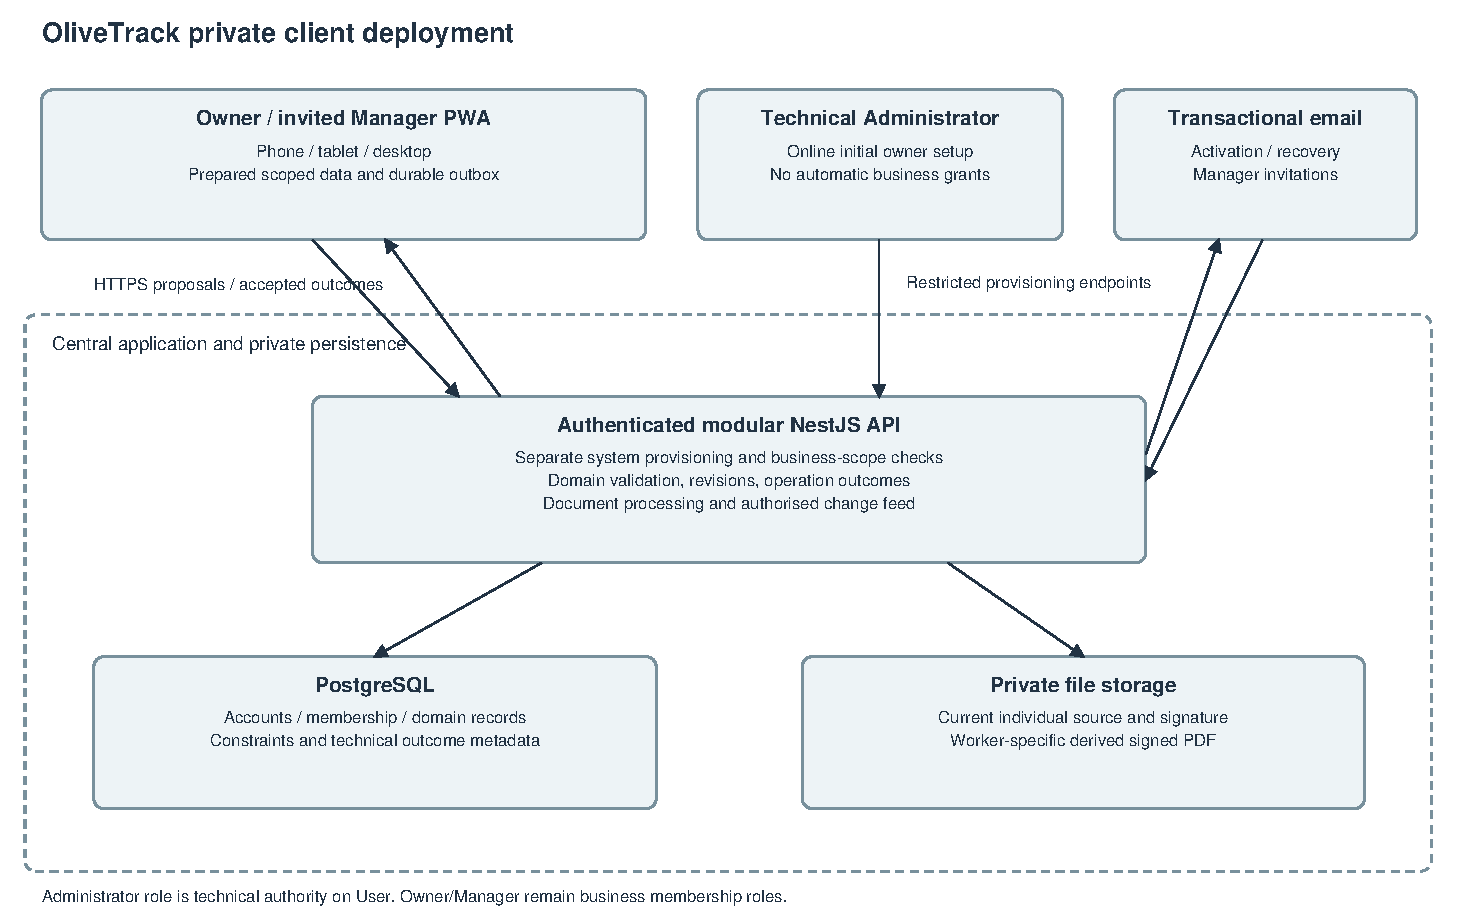
\includegraphics[width=0.98\linewidth]{solution-components-review.pdf}
\caption{Component responsibilities and separate technical/business authority. Restricted provisioning and scoped business endpoints use the same modular API. Device-local proposals and private central storage remain separate trust boundaries; no browser has direct database access.}
\label{fig:solution-components}
\end{figure}\FloatBarrier

\subsection{Components and Responsibilities}
\subsubsection{Client Application and Local Storage}
The React PWA uses Vite for builds and Tailwind CSS for responsive
presentation. A service worker prepares the application shell; IndexedDB holds
the authorised local dataset, file availability metadata and durable outbox.
Browser caching alone is not a business-operation queue. Save each supported
proposal and its outbox entry atomically before reporting local success.

Prepare only the required scope and permitted source versions/files. Include
insurance consultation and selected-version signing under their grants, rather
than excluding all contracts or insurance from offline use. Prepared financial
consultation, entry, correction and PDF output also follow their grants. Record
file readiness separately from structured-record acceptance. Preserve pending
dependencies through normal app closure and restart while browser storage remains
intact; clearing storage or losing a device can destroy exclusively local work.
Storage checks and warnings follow \identifier{AOC-05}.

The interface uses the business and synchronisation states in
Section~\ref{sec:sync-states}. A generic failure label must not obscure the
difference between transmission failure, rejection, conflict and an uncertain
server outcome. Normal field interaction remains simple, with recovery detail
shown when action is needed, as defined in Section~\ref{sec:offline-interaction}.
Browser-background execution is not assumed to be continuously available: retry
when execution and connectivity permit, and provide an explicit retry/review path.

\subsubsection{Identity and Delegated Access}
User identifies the account; WorkspaceMembership carries the contextual role and
AccessGrant carries permitted operations and owner-assigned responsibility scope.
Each owner has one business workspace. A real person working for different owners
may have separate Worker records; no global worker directory or cross-business
identity merge is introduced. The Owner role does not prove legal property title.

Technical account provisioning validates the separate administrator system role.
The administrator receives no operational grants automatically. Every protected
business API read, write, export and file request validates account, membership, operation and scope. Never trust a workspace identifier or role sent
by the browser. Preserve the reviewed manager defaults and mandatory scoped
insurance consultation in Section~\ref{sec:permission-defaults}; other document
and financial operations retain their independent grants. Property-based scope
includes parcels and current/future campaigns, permits multiple managers and
filters multi-property views to authorised contributions. Explicit worker
availability does not grant visibility of other-property work; see
\decisionref{Q-AA-02}.

Prepared offline authorisation expires 15 days after the latest successful online
permission validation. It is distinct from online-session expiry and 30-day
accepted-cache cleanup. Logout blocks local access while protecting recoverable
pending proposals; it does not indiscriminately erase the outbox. Offline devices
cannot receive immediate revocation or remote wiping. Central access checks,
reconnection and the local expiry gate enforce the applicable boundary. The
trusted-time, local protection and restricted owner-review mechanisms remain
subject to the existing security decisions.

\subsubsection{Business API and Domain Modules}
The Node.js/NestJS API is organised into cohesive modules in one backend
application. This modular structure does not require independently deployed
microservices. Module responsibilities follow the current data model:

{\compacttable
\begin{longtable}{L{0.27}L{0.73}}
\caption{Proposed backend modules.}\label{tab:backend-modules}\\
\toprule\rowcolor{TableHeader}
\textbf{Module} & \textbf{Responsibility}\\\midrule\endfirsthead
\toprule\rowcolor{TableHeader}
\textbf{Module} & \textbf{Responsibility}\\\midrule\endhead
\multicolumn{2}{r}{\footnotesize\itshape Continued on next page}\\\endfoot
\bottomrule\endlastfoot
Access and workspaces & Initial owner provisioning, activation/recovery, invitations, memberships and operation-specific grants.\\\midrule
Properties and campaigns & Properties, optional parcels, coverage, explicit execution start, closure, reopening and archival rules.\\\midrule
Workforce and work & Identified workers, capabilities, optional plans, daily attendance, actual assignments, periods, tasks and breaks.\\\midrule
Worker documents & Uploaded/generated source versions, one worker per document, templates, signatures, renditions and retention.\\\midrule
Harvest logistics & Delivery-associated transport, actual load origins, driver/vehicle references and weighing tickets.\\\midrule
Analyses and indicators & Delivery analyses, current ticket-reported amounts, assigned-weighted yield and scoped indicators/PDF summaries.\\\midrule
Synchronisation & Operation outcomes, revisions, ordered dependencies, authorised change feed and reviewed conflict/recovery paths.\\
\end{longtable}}

\subsubsection{Shared Rules and Central Persistence}
A shared TypeScript package provides types and pure validation/calculation
functions used by client and server. Local results are previews while acceptance
is pending. Shared code does not replace server authorisation, complete-data checks
or database integrity. The server recalculates and validates accepted changes.

PostgreSQL stores the model in Section~\ref{sec:data-architecture}. Use foreign keys, uniqueness,
checks, transactions and suitable cross-record enforcement. Same-workspace
references, actual-period non-overlap and exclusive accepted campaign execution
need more than ordinary independent row checks. Keep technical idempotency and
deletion metadata separate from permanent business field history.

Each delivery has at most one ticket and one analysis, and each ticket has one
current reported monetary value. A reported final amount replaces its provisional
predecessor; ordinary corrections retain current values. Store reported values
and units, with validated source metadata and independent printed processing
duration. KILOS ASIGNADOS supplies accepted assigned kg, total kg is separate and MEDIANERIA is the accepted percentage rather than laboratory yield; no assumed penalty tariff or repeated deduction is applied.
Calculate aggregates from eligible sources under Section~\ref{sec:calculation-rules}.
Weights, yields and monetary totals include only Delivered, non-cancelled
deliveries with the required inputs. Local arrival can update provisional local
indicators; central totals require accepted arrival and source records.

\subsubsection{Files, Generation and Signing}
Files are required architecture components. Keep them private in an object store
or equivalent protected service, with authorised access through the API or
short-lived scoped links. A private S3 bucket is a deployment candidate; document workflows do not depend
on selecting that provider. Validate each file request and keep
secrets and reusable privileged credentials out of the browser bundle.

Maintain immutable source identities/content hashes, document versions, per-worker
signature evidence and worker-specific derived signed PDFs. Capture the worker's
review and confirmation for the selected version; the operator's account identifies
the facilitator and does not replace the worker as signer. A later source version
needs its own signing event. Template generation under \identifier{UC-20} and
\identifier{FR-063} produces reviewed unsigned source versions; available templates
use the four supplied Spanish forms in Table~\ref{tab:source-forms}, preserving their wording under \decisionref{Q-DOC-01}. Decision-bearing forms add a typed choice
to worker/version evidence, committed atomically with signature acceptance and
rendered on the worker-specific PDF. Generation leaves the choice unselected. The workflow does not issue official identity
or work-permit evidence.


Retention follows \identifier{BR-026} and Section~\ref{sec:data-lifecycle}: keep
each current document source, signature and PDF until a complete replacement is accepted,
then delete the old graph for every category without inheritance or a history view.
Explicit ticket/analysis/value-attachment replacement also deletes the previous file
after success. Failed uploads preserve the current source/evidence. Coordinate this
with minimal deletion/idempotency metadata, private object storage and safe retries;
a database transaction alone does not atomically delete an object-store file.
The 10~MB PDF/JPG/JPEG/PNG policy applies to uploads. A captured mark and digest
do not certify legal identity; manual privacy/operational procedures remain separate
deployment preparation. The team implements/tests protection and recovery within
the agreed current-only and exact-source signing policies.

\subsection{Main Interaction Flows}
\begin{enumerate}
\item \textbf{Connected preparation.} Authenticate and validate permissions, then
prepare selected reference data, schedules and permitted files. Account/access,
property structure, campaign creation/coverage/closure/reopening, existing-worker
administration, source-version management and generation use connected workflows.
\item \textbf{Field entry.} Review and confirm a supported operation, durably save
its local proposal and dependencies, and show its actual save state. Prepared
explicit campaign starts and identified same-day worker creation are supported
offline exceptions; they do not make all administration available offline.
\item \textbf{Central acceptance.} Authenticate again as needed, check current
authority, operation identity, revision, dependencies and business rules, and commit
the outcome consistently. Reconcile the result without duplicate business effects.
\item \textbf{Review and completion.} Consult authorised incoming changes and
indicators, resolve conflicts explicitly and complete late source information.
Campaign closure/correction exceptions follow the use cases and rules, not an
append-only restriction on all business records.
\end{enumerate}

\subsection{Offline Operation and Synchronisation}
\label{sec:offline-sync}
\label{sec:offline-synchronisation}
The proposed protocol separates durable local proposals from centrally accepted
records. Prepared datasets and local/central storage responsibilities are described
in Section~\ref{sec:data-local-central}. Authentication limits, recovery mechanisms
require technical validation even where their behaviour and selected stack are approved.


\subsubsection{Local Proposals and Ordered Dependencies}

Each proposed operation is identified by a stable \texttt{operation\_id}, origin
User, Workspace, entity type and ID, and operation kind.
For validation, it also carries the payload, base revision for updates, dependency
IDs and client recording time. The local outbox uses the states in
Section~\ref{sec:sync-states}, with separate retry detail.
Client timestamps do not prove central acceptance or prior authorisation.
Use stable client-generated record identifiers for offline creation; the selected
UUID generation method must be consistent across devices and server.

The selected local store must persist each business proposal and its outbox entry
atomically before the application reports a successful local save. Show local confirmation separately from acceptance.
Submit dependencies first: a delivery before its ticket, a version before signing,
and accepted metadata/file readiness before dependent references. Basic worker creation and explicit campaign start are supported exceptions.
Queue a worker before attendance, assignments and driver references. Individual
document creation/source acceptance is online and requires that worker first;
prepare that accepted source before offline signing. Queue campaign start before dependent
execution records. Administration of existing profiles and property creation remain online.


Use one stable client-generated Worker UUID and operation UUID through local
creation and acceptance. Pending references must not be replaced by an unrelated
identity if a duplicate warning appears. Resolve an existing/new identity only
through an explicit reviewed procedure that preserves work, document associations
and files; no automatic merging or cross-business lookup is introduced.

An explicit start proposes Planned to In progress. The server validates authority,
actual dates and competing execution atomically before accepting dependent records.
Concurrent offline starts on one area cannot both become accepted; keep the rejected
or conflicting start and its dependencies recoverable. A device timestamp is not
an authoritative proof of an exclusive reservation.


\subsubsection{Central Acceptance, Conflicts and Incoming Changes}

For each request: authenticate the account, determine the operation workspace,
validate current authority, check operation identity and compare its fingerprint,
then validate base revision and domain invariants in a transaction. A reused ID
with different content is not the same retry. Commit the business change and its
idempotency outcome consistently, and return affected identities/revisions.
An outcome ledger stores minimal replay status, not a permanent full copy of every
old business row. Retain minimal operation outcomes for 90 days after processing
and change/deletion-feed markers for 90 days. Support the preceding client/payload
version for 30 days after a release. Server-issued validity context must route
stale requests to refresh/reviewed recovery; missing expired metadata never proves
that a request is new. Validate safeguards against duplication and resurrection.

An uncertain transmission triggers operation-status checking or safe retry.
Never assume that timeout means no central change. A stale base revision produces
a conflict, not Last Write Wins. Authorised users compare accepted values and the
proposal, then keep accepted data or resubmit a reviewed correction for validation.


The server supplies only changes the account may receive, using a proposed durable
cursor. Apply business changes, deletion markers and cursor advancement consistently.
A deletion marker is a technical synchronisation fact, not a field-change history.
After access reduction, the client removes inaccessible prepared data without
submitting it through another account. Beyond the valid change-retention window,
refresh authorised data rather than silently missing old deletions.

Track attachment upload separately from structured-record acceptance. Keep failed
uploads recoverable and do not expose an unavailable object as stored. A replacement
version becomes current only once its source is available. Offline retention cleanup
must not revive deleted versions when a pending signature reconnects.


\subsubsection{Access Expiry, Logout and Recovery}

Logout blocks local access but preserves recoverable pending work in account-isolated
protected storage. Renewed authentication is required for normal recovery.
Revocation is enforced online and on reconnection or offline expiry; no instantaneous
remote wipe of disconnected devices is asserted.

Existing pending manager proposals may enter a restricted Owner-review workflow
without restoring manager workspace access. Preserve origin and reviewer, and run
all campaign, date, revision and dependency checks on acceptance. Owner acceptance
supplies new explicit authority; client timestamps cannot establish pre-revocation
creation. The origin account authenticates only for restricted submission, without
normal workspace access. Concrete protected transport/quarantine/expiry remains
a verification task. Signing-source eligibility cannot be overridden by approval.


Enforce \hyperref[br:002]{\identifier{BR-002}} through a local gate storing the last successful
online permission-validation instant and expiry. Cached use and cleanup cannot
renew it. Protect this context against simple clock rollback; the trusted-time
mechanism remains a security design decision. Expiry blocks consultation/new
operations but preserves protected recoverable proposals until online revalidation.
It does not deliver server changes; the authorised change feed does that.

The routine presentation follows Section~\ref{sec:offline-interaction}. A simple
status does not replace durable outbox storage, dependency checks or idempotency.
Local protection and expiry follow \identifier{PRV-03}/\identifier{AOC-02}; the final mechanism remains
under \decisionref{Q-DOC-07}. Warning/retry timing and concrete local security
mechanisms remain pending; approved session/backup/recovery/availability targets
are specified by their owning NFRs. \identifier{REL-08} and \decisionref{Q-NFR-06} govern restricted
owner-review recovery, not a normal submission bypass.

\subsubsection{Local Indicators and Operation Boundaries}

Use the last accepted available baseline plus identifiable local proposals: create
once, replace on update and remove the previous contribution on local removal.
Label affected values provisional and disclose missing/partial scope and last sync.
Apply the same Delivered, non-cancelled eligibility to all delivery-based totals.
A local arrival confirmation enables eligible contributions in the provisional
view; pre-arrival source data remains in detail awaiting receipt confirmation.
Central totals use only server-accepted arrival confirmations and source values.
Rejected proposals do not remain part of accepted totals. Never imply knowledge of
other-device changes since last synchronisation. Offline PDF may include authorised prepared financial information and records generation time, scope, freshness, missing information and pending data. Financial source provisional/final status is separate from synchronisation status.



The outbox accepts only the operations supported in
Section~\ref{sec:non-functional-requirements}; connected administration and source
generation use online endpoints. Prepared datasets/file manifests enforce the
operation and complete-file restrictions in Section~\ref{sec:conceptual-files}.
Coordinate source, evidence and rendition cleanup with protected signing operations;
exclusively local signatures may require \decisionref{Q-DOC-04} resolution.
Cancellation remains a domain update in the change feed, rather than a deletion
marker, preserving dependencies while removing indicator contributions.


\subsection{Deployment and Operation}
\subsubsection{Proposed Hosting Arrangement}
Separate static PWA delivery, the application API, PostgreSQL and private file
storage. The contribution suggests AWS in an EU region: S3/CloudFront for the
application, an evaluated container service for the API,
RDS for PostgreSQL, private S3 files, Secrets Manager and CloudWatch.
This is an example topology under \decisionref{Q-ARCH-02}; it is not a procurement
decision, a free-tier guarantee or evidence of operational availability. Evaluate
an academic/managed alternative if necessary without weakening access, integrity
or document controls. Application-managed authentication is selected; choose the transactional email provider separately.

The EU-region preference does not itself demonstrate privacy compliance. Review
processing locations, provider roles, transfers and costs under
\decisionref{Q-NFR-03} and \decisionref{Q-ARCH-02}. Use synthetic or appropriately
anonymised demonstration data until the processing basis for real personal data
has been established. Configure encrypted transport/storage, least-privilege
service access and secret management against Section~\ref{sec:nfr-security}.

\subsubsection{Code Organisation and Delivery}
The proposed monorepo separates client, server and shared contracts/rules.
Pin dependencies and review generated or contributed code under the same standards.
GitHub Actions can run build, lint, unit/integration checks and migration validation
before merge/deployment. Docker is proposed for reproducible server packaging;
choose one infrastructure-as-code approach, such as Terraform or AWS CDK, only
if it fits the team's capacity. These engineering mechanisms remain planned.

Changes to local schemas, service workers and API payloads must preserve pending
work and account for older cached clients. Store the client/payload version with
sync requests and reject unsupported formats recoverably. Do not force an update
that clears queued work. Use reviewed migration and rollback procedures; an old
application release is usable only with a compatible schema and payload contract.
The approved 30-day preceding-client compatibility policy is specified in \identifier{REL-07} and
\decisionref{Q-NFR-02}.

\subsubsection{Operational Verification}
Assign monitoring, incident, backup and restore responsibilities before operational
use. Managed services do not remove application-level configuration or restore
testing. Approved availability, daily/14-day backup, RPO/RTO and performance
targets are specified in the owning NFRs; do not create independent architecture
targets or imply they have been measured. Central backups cannot recover changes that never left a lost device.
Security audit events have a separate purpose and retention policy from business
correction history.

Measure rendering, durable local saving, central acknowledgement, structured replay
and file transfer separately. Synthetic probes must not expose worker data or
disable supported offline entry. Validate phone/tablet usability and recovery
feedback under Section~\ref{sec:nfr-usability} and \identifier{AOC-06}. Test
retries, concurrent edits, offline starts/new workers, storage interruption and
source/signature retention before claiming the corresponding behaviour works.
Section~\ref{sec:risk-management} records the project risks affecting delivery.

\subsection{Architecture Decisions and Remaining Validation}
The reviewed specification already separates planned and actual work, local
confirmation and server acceptance, source files and signed renditions, and
business corrections and technical replay metadata. Stable identities, idempotent
effects and optimistic revision checks with explicit conflict review are retained.
Last Write Wins is not an alternative conflict policy in this baseline.

\decisionref{Q-ARCH-01} records the selected stack and the outstanding tested vertical slice; \decisionref{Q-ARCH-02} covers hosting, service selection,
costs and operating ownership. These do not reopen the included manager, prepared
document/signing flows, authorised offline finance or one-ticket/one-analysis rules.
Property scope, owner-authorised recovery and metadata lifetimes are decided.
Concrete local encryption/key handling, trusted-time enforcement, safe expired-context
recovery and legal/operational signing suitability retain the specific validations
in Section~\ref{sec:uc-open-decisions}.
Implementation and verification target the single final delivery under
\decisionref{Q-SCOPE-01}; internal technical slices are development steps.

\paragraph{Rationale and trade-offs.}
The following decisions explain the proposal's main quality drivers. They record
design reasoning, not comparative benchmark results or final procurement approval.
{\compacttable
\begin{longtable}{L{0.23}L{0.45}L{0.32}}
\caption{Architecture rationale, trade-offs and validation needs.}\label{tab:architecture-rationale}\\
\toprule\rowcolor{TableHeader}
\textbf{Proposed choice} & \textbf{Reason / requirement driver} & \textbf{Trade-off / validation}\\\midrule\endfirsthead
\toprule\rowcolor{TableHeader}
\textbf{Proposed choice} & \textbf{Reason / requirement driver} & \textbf{Trade-off / validation}\\\midrule\endhead
\multicolumn{3}{r}{\footnotesize\itshape Continued on next page}\\\endfoot
\bottomrule\endlastfoot
Responsive PWA with IndexedDB outbox & One phone/tablet interface and prepared field continuity; atomic local proposals support \identifier{FR-034} and \identifier{AOC-03}. & Browser storage and execution limits require device tests; protection and trusted time remain under \decisionref{Q-DOC-07}.\\\midrule
Modular TypeScript API and shared pure rules & Modules follow domain responsibilities; shared previews reduce divergent calculations, while the server enforces \identifier{REL-03}. & Shared code does not supply authority or concurrency guarantees. Validate the selected stack through the technical slice under \decisionref{Q-ARCH-01}.\\\midrule
PostgreSQL transactional acceptance & Relationships, uniqueness and serialised validation support single tickets/analyses, attendance and exclusive execution. & Cross-record checks need a tested transaction/locking design, not only independent row checks.\\\midrule
Stable operations and optimistic revisions & Safe retries and explicit conflict review preserve \identifier{REL-01}/\identifier{REL-02} without silent last-write-wins. & Adds dependency and recovery work; expired-context safeguards and owner-authorised recovery remain verification tasks.\\\midrule
Private object storage plus relational metadata & Keeps source files, signature evidence and derived PDFs distinct under \identifier{SEC-08} and \identifier{BR-026}. & Database/file readiness and cleanup need recoverable coordination; provider/cost and retention are separate decisions.\\\midrule
Managed hosting candidate & Separates application delivery, API, database and files while supporting configurable backup/monitoring. & Compare an affordable deployment against the agreed NFRs; AWS is an option under \decisionref{Q-ARCH-02}, not a free or approved service guarantee.\\
\end{longtable}}


\paragraph{Required technical slice.}
Authenticate and prepare an authorised campaign/worker; durably save field work
offline; close/reopen the PWA and verify persistence; reconnect and accept centrally;
retry the same operation without duplicate effects; then create a competing revision
and verify explicit conflict recovery. Include stale-context recovery, local
encryption/key lifecycle and fail-closed expiry boundary checks before claiming
the corresponding architecture is feasible on the supported devices.

\paragraph{Supplied skeleton and implementation gap, 24 November.}
The supplied archive contains npm workspaces, NestJS/Prisma, PostgreSQL Compose,
React/Vite/Tailwind PWA configuration and a Task-only Dexie/outbox example. Its
schemas and migrations model Task/AppliedMutation, its manifest identifies a task
application and its example sync chooses newer client timestamps. It provides
starting files to adapt and verify under the task catalogue. Domain contracts,
scoped authentication/provisioning, schema migrations and explicit revision conflict
handling still need implementation. Replace the example LWW path before accepting
agricultural mutations under this baseline. Validate source readiness, permissions,
retained pending work and supported PWA update behaviour through the technical slice.

\FloatBarrier
\section{Data Architecture}
\label{sec:data-architecture}
This section describes the proposed entities, relationships, integrity constraints
and storage representations. Sections~\ref{sec:use-cases}--\ref{sec:business-rules}
define behaviour; this model must implement those constraints. Types, indexes and
technology choices remain design proposals where not yet agreed.

The companion field reference is compiled from
\nolinkurl{data-architecture-reference.tex}, using
\nolinkurl{technical/data-architecture/data-dictionary.tex}. It supplies field-level
detail omitted from this summary and must be versioned with it. Any conflict with
the requirements requires an explicit correction or decision, not silent precedence.

\subsection{Conceptual Data Model}
\label{sec:data-conceptual}
The proposed model contains 33 entities/associations, including the new WorkerAvailability access association. The complementary ER views show one
model, with contextual entities in grey and endpoint cardinalities explicitly
labelled. Each delivery may have at most one weighing ticket and one analysis,
both of which may be recorded later. ManagerInvitation and AccessGrant
are included. DocumentTemplate and DocumentRendition support the agreed \identifier{UC-20} and
signed worker-specific PDF output. Authentication challenges, outbox operations
and recovery ledgers are technical persistence, not additional business actors.

\subsubsection{Accounts and Business Access}
User is the application identity with a separate administrator/standard system role;
Worker is a business-specific person with no
required login. Workspace separates one owner's properties, campaigns and records.
WorkspaceMembership carries the contextual Owner/Manager role; each active
workspace has one Owner and an account owns at most one workspace.
ManagerInvitation records recipient and reviewed initial grants; acceptance requires
the intended verified account. AccessGrant records actual operations and scope,
including the mandatory insurance constraint. Revocation preserves author/initiator
references. Email verification challenges do not change the User id or ownership.
Workspace stores its business timezone. AccessGrant is keyed by membership,
operation and required property; scopes include parcels and current/future campaigns.
WorkerAvailability links explicitly available workers to manager membership before
scoped work exists; other relevant workers follow authorised scoped records.
It confers no other-property work visibility. Business closure and ownership
transfer are excluded. Account/data erasure requests require the separate privacy
procedure under \decisionref{Q-AA-07}; the model introduces no closure workflow.
Figure~\ref{fig:er-access} summarises the access relationships.

\begin{figure}[!htbp]\centering
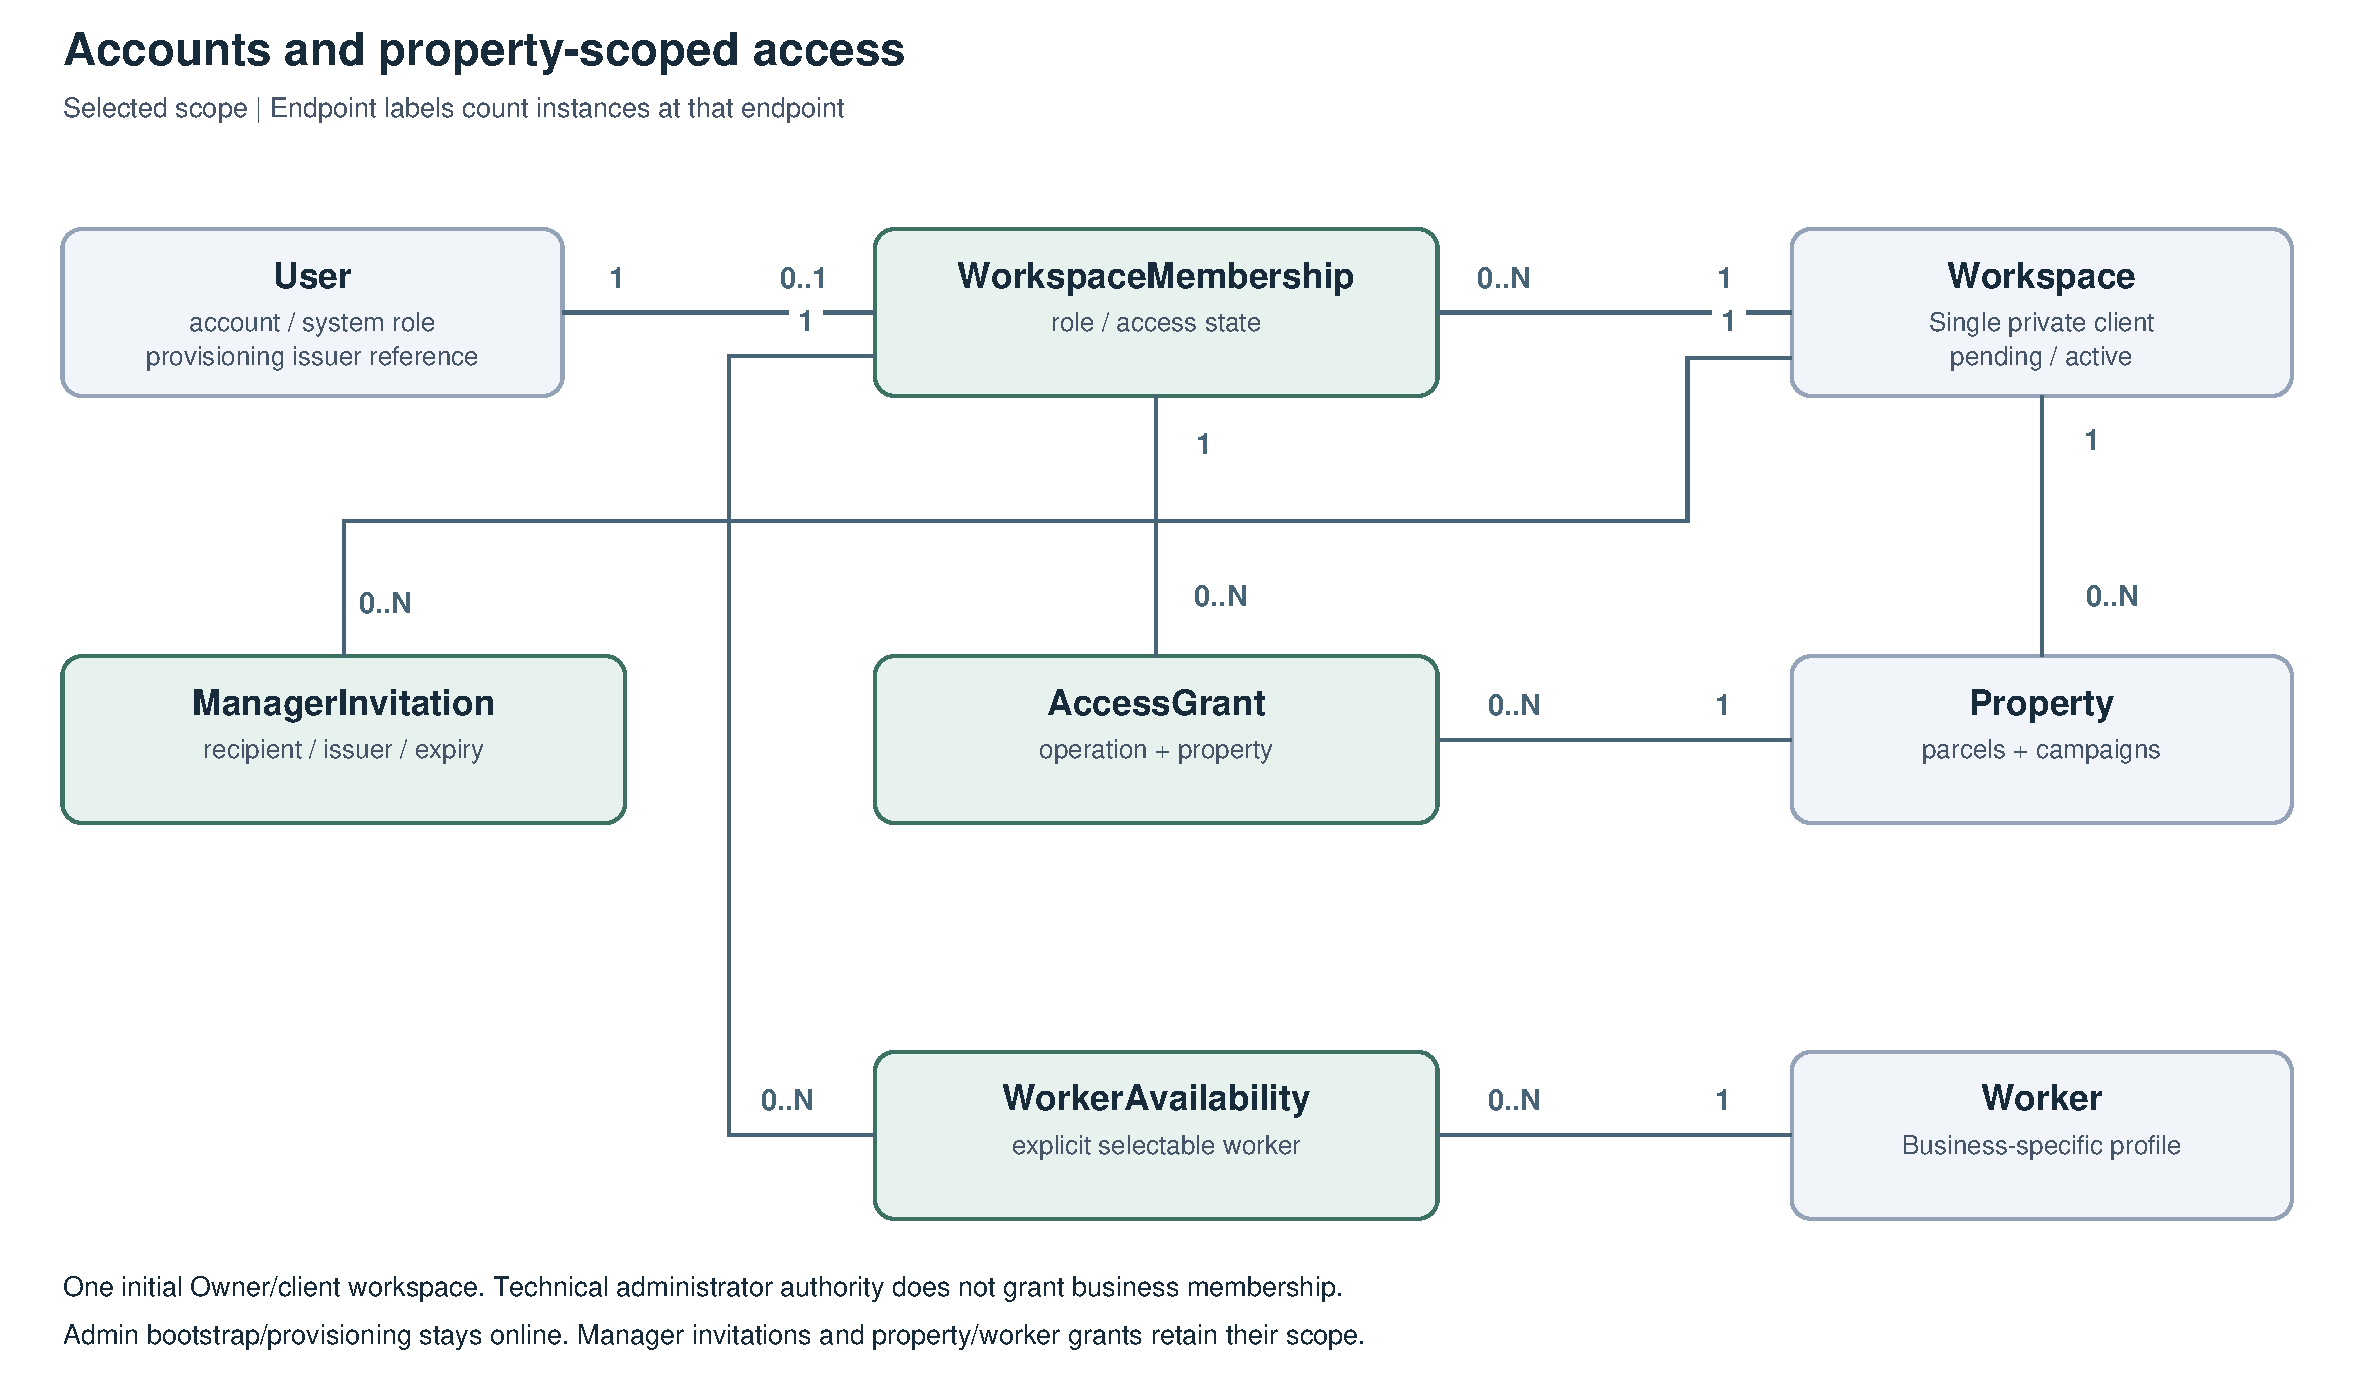
\includegraphics[width=\linewidth]{er-access.pdf}
\caption{Included account, membership, invitation and owner-configured access relationships.}
\label{fig:er-access}
\end{figure}

\paragraph{Provisioning.}
The administrator system role enables initial owner and workspace setup and activation
support only. Owner/Manager remain the operational membership roles. Bootstrap the
first administrator through deployment configuration, with no public administrator
signup. A nullable administrator reference on the provisioned owner records who
initiated setup. The owner workspace and membership remain pending until verified
activation; manager memberships still arise through accepted owner invitations.
The single-client deployment guard prevents a second initial owner/workspace.

\subsubsection{Properties, Parcels and Campaign Coverage}
\label{sec:conceptual-properties}
Property and HarvestCampaign belong independently to a Workspace. Parcel is an
optional reusable division of a Property. CampaignCoverage links a campaign to
one or more whole properties or selected parcels, allowing a campaign to span
several properties without duplicating their records.
Figure~\ref{fig:er-properties-campaigns} shows the coverage relationships.

\begin{figure}[!htbp]
\centering
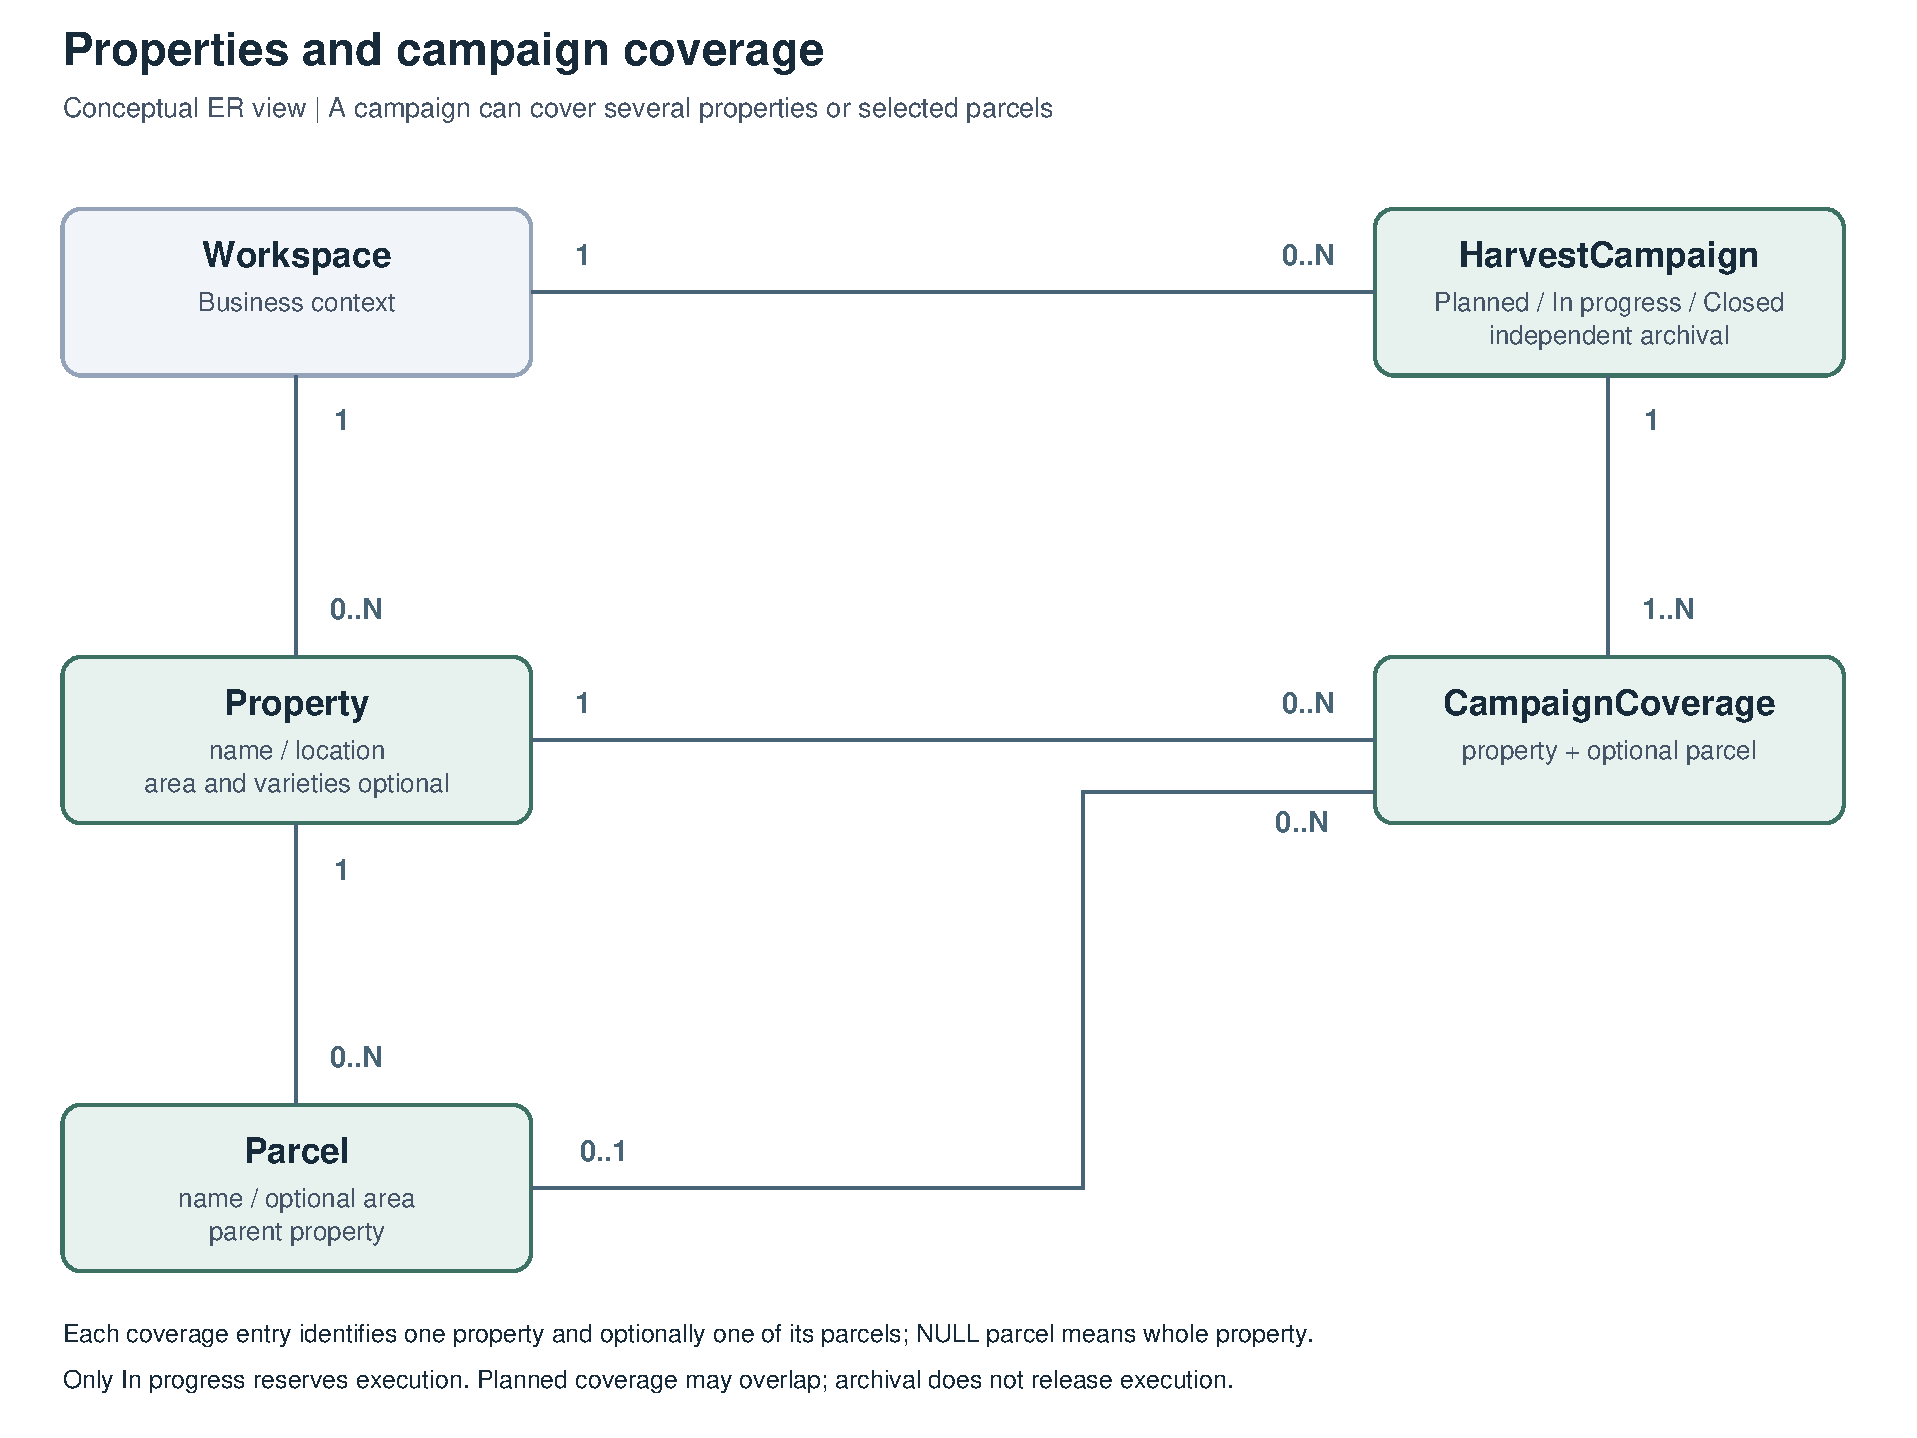
\includegraphics[width=\textwidth]{figures/er-properties-campaigns.pdf}
\caption{Properties, optional parcels and campaign coverage. A coverage entry always identifies a property and optionally one of its parcels.}
\label{fig:er-properties-campaigns}
\end{figure}

A coverage entry always identifies a property and optionally one of its parcels;
an absent parcel denotes whole-property coverage. Operational area references use
the same representation. This preserves the difference between property-level
and parcel-level information when divisions are added later.

HarvestCampaign stores planned start, actual start and actual end separately.
Lifecycle and archival are separate fields because execution/closure govern dates,
while archival controls normal-list visibility. CampaignCoverage is the set against
which start/reopening and In progress coverage changes enforce
\hyperref[br:008]{\identifier{BR-008}}. This cross-record constraint needs transactional
validation; the ER relation alone cannot enforce exclusive execution.

\subsubsection{Business Worker Records}
\label{sec:conceptual-workers}
Worker belongs to a Workspace and retains a stable internal UUID across planning,
attendance, work, driving, document associations and signatures. Mandatory fields
are full name, telephone, official identification type, issuing country and number;
keep the number as text, separately from the UUID and from optional fiscal data.
The type/country/number tuple supports non-unique same-business duplicate lookup;
it is neither a primary key nor a global uniqueness constraint. Identification types are DNI, NIE and Other; Other requires a description. The issuing country is recorded, while country-specific document-format validation is excluded under \decisionref{Q-ID-01}. Offline proposals and their
dependants retain the same UUID through acceptance, as described in
Section~\ref{sec:offline-sync}. Profile updates preserve identity and links;
machinery capability is stored separately from actual tasks.

The profile's activity history queries DailyAttendance, ActualWorkAssignment,
WorkPeriod and WorkBreak under the same worker identity and authorised scope.
Daily and selected-period totals are derived under \identifier{FR-023(c)}; no
additional worker-hours table or copied profile total is required. Corrections
refresh the view from current work records.

\subsubsection{Work Planning, Attendance and Actual Work}
\label{sec:conceptual-workforce}
The model separates expectations, daily presence and actual campaign participation.
WorkPlan groups one campaign's assignments for a working date. PlannedAssignment
identifies a worker and area, with optional PlannedWorkPeriod and PlannedBreak
records. These tables retain the proposal independently of subsequent actual work.
Figures~\ref{fig:er-planning} and~\ref{fig:er-actual-work} show planning and actual work,
respectively.

\begin{figure}[!htbp]
    \centering
    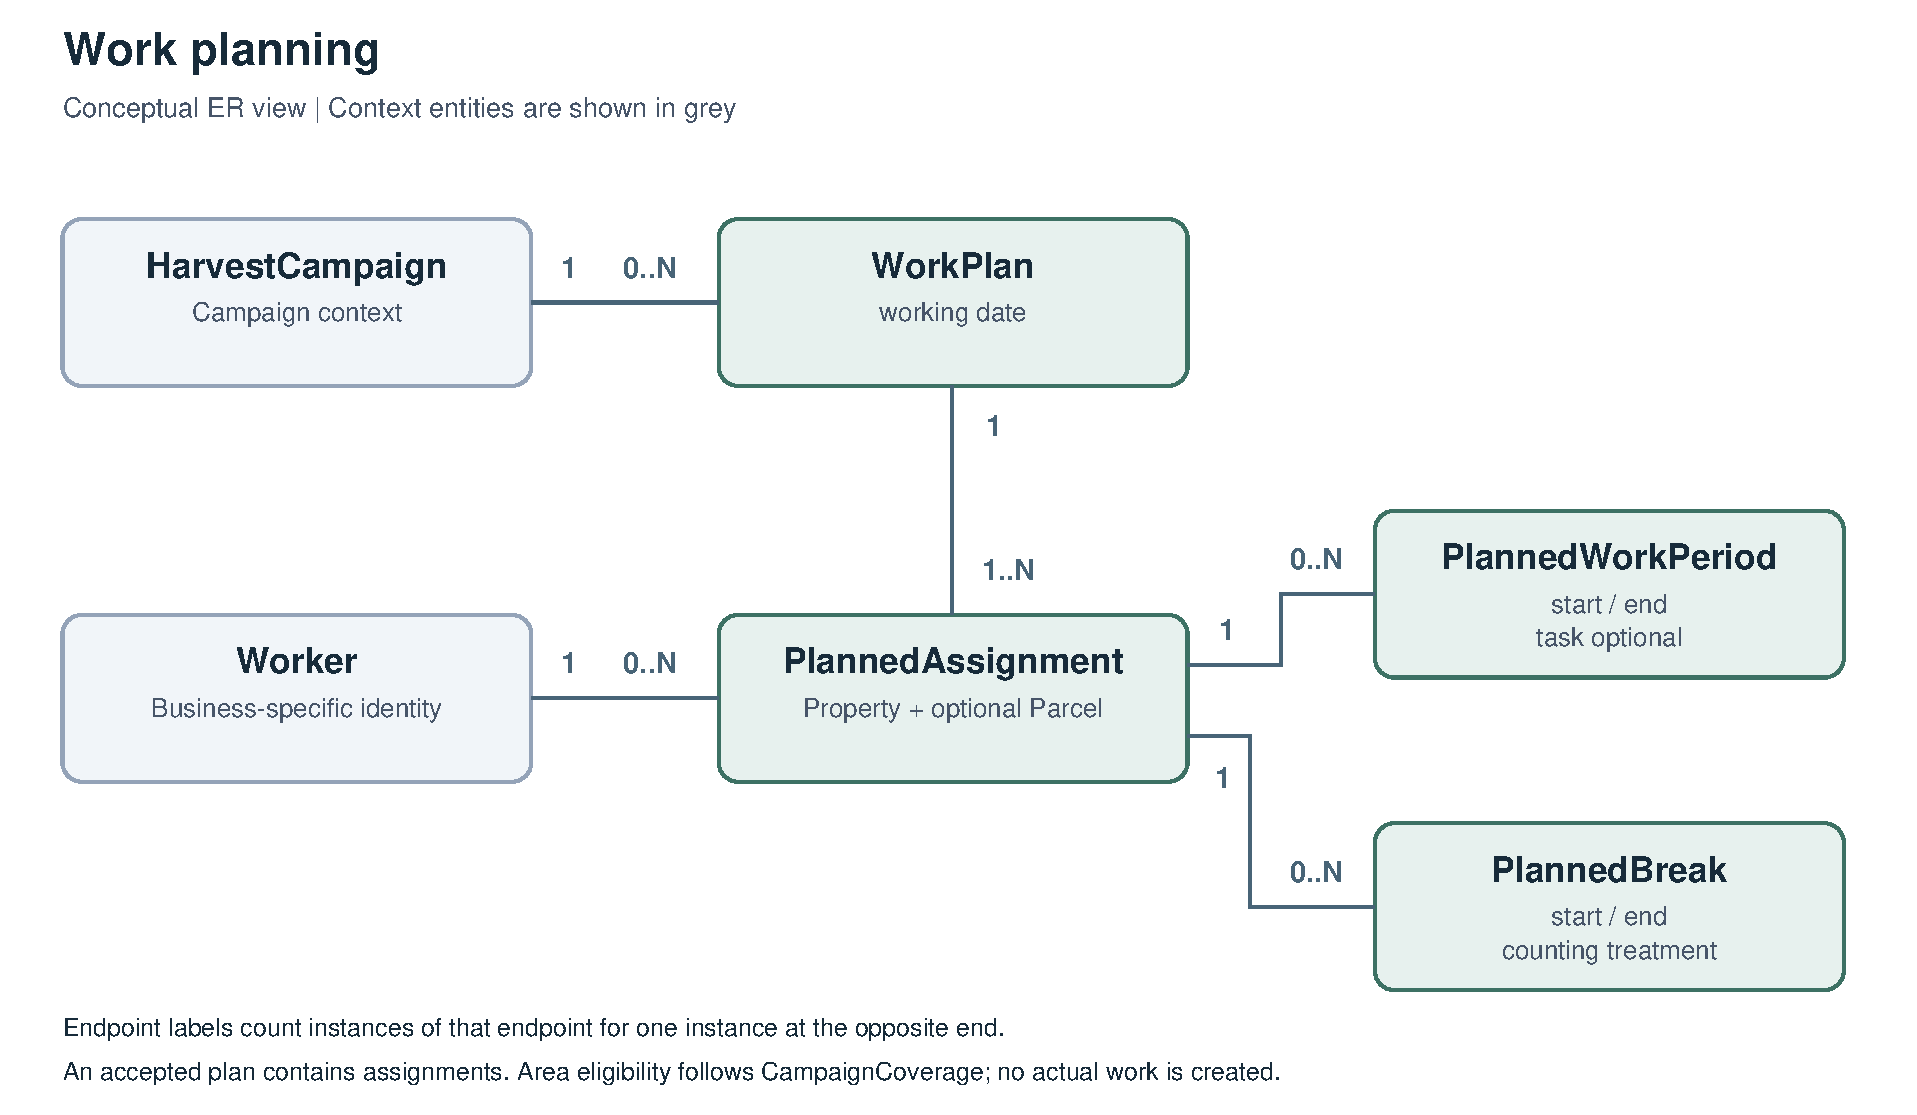
\includegraphics[width=\textwidth]{figures/er-planning.pdf}
    \caption{Conceptual relationships for work planning.
    Context entities are shown in grey; area references are summarised.}
    \label{fig:er-planning}
\end{figure}

\paragraph{Daily presence and campaign participation.}
DailyAttendance identifies one worker and working date within a workspace, without
a campaign reference. ActualWorkAssignment supplies the campaign and area context.
This supports one daily attendance decision across several campaigns and records
participation before hours or tasks are complete. An actual assignment may refer
to a source PlannedAssignment, but no mandatory one-to-one correspondence is imposed.

\begin{figure}[!htbp]
    \centering
    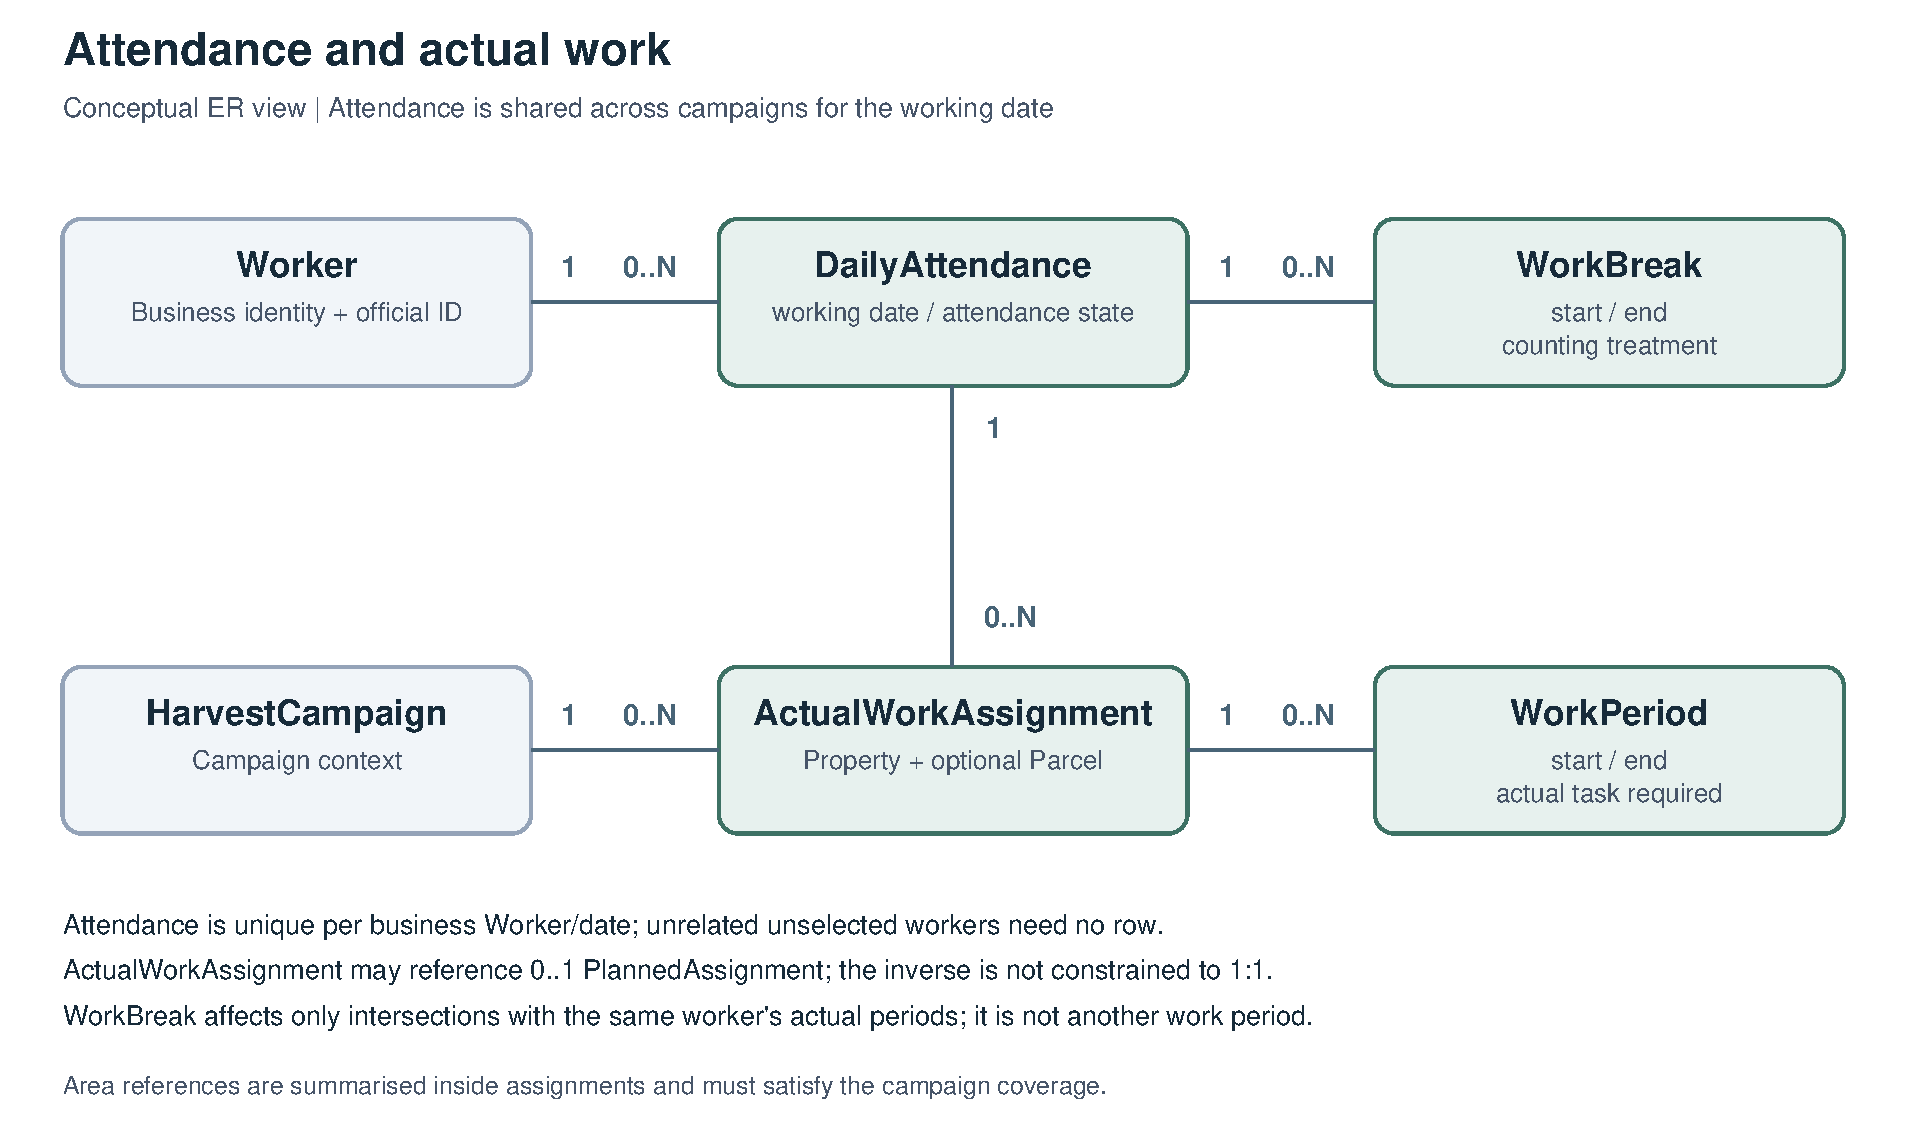
\includegraphics[width=\textwidth]{figures/er-actual-work.pdf}
    \caption{Conceptual relationships for daily attendance and actual work.
    The optional reference to a planned assignment does not impose a one-to-one correspondence.}
    \label{fig:er-actual-work}
\end{figure}

\paragraph{Intervals and breaks.}
WorkPeriod belongs to an actual assignment; WorkBreak belongs to daily attendance.
The latter placement lets a worker's break intersect consecutive task or campaign
periods without duplicating it. Complete start/end timestamps support intervals
crossing midnight and cross-campaign overlap checks. Missing hours are represented
by the absence of complete periods; each confirmed complete period requires
its actual task. An incomplete assignment is not converted into zero hours.

Planning and confirmation conditions are defined in \hyperref[br:017]{\identifier{BR-017}}--\hyperref[br:021]{\identifier{BR-021}};
the counted-time formula is in Section~\ref{sec:counted-working-time}.
Completion and correction use Sections~\ref{sec:completion-correction} and~\ref{sec:work-corrections}, without a separate
entity for every historical field value.

\paragraph{Expected versus unrelated workers.}
DailyAttendance is sparse: it does not require a row for every worker/date. Derive
expectations from selected/planned or actual assignments under
\hyperref[br:018]{\identifier{BR-018}}. This avoids recording non-selection as absence. Pending
records reference locally created Worker UUIDs without creating a second daily
attendance after acceptance.

\subsubsection{Deliveries, Loads and Cooperative Results}
Delivery belongs to one campaign and has one associated TransportRecord, with a
registered Worker driver. OliveBatch stores one actual source property and optional
parcel, with known source quantities separate from official ticket weights.
TransportRecord may retain a transport-document reference and declared origin;
these do not allocate a mixed load or make parcels mandatory.
Figure~\ref{fig:er-deliveries} shows the delivery and source-result relationships.
\begin{figure}[!htbp]\centering
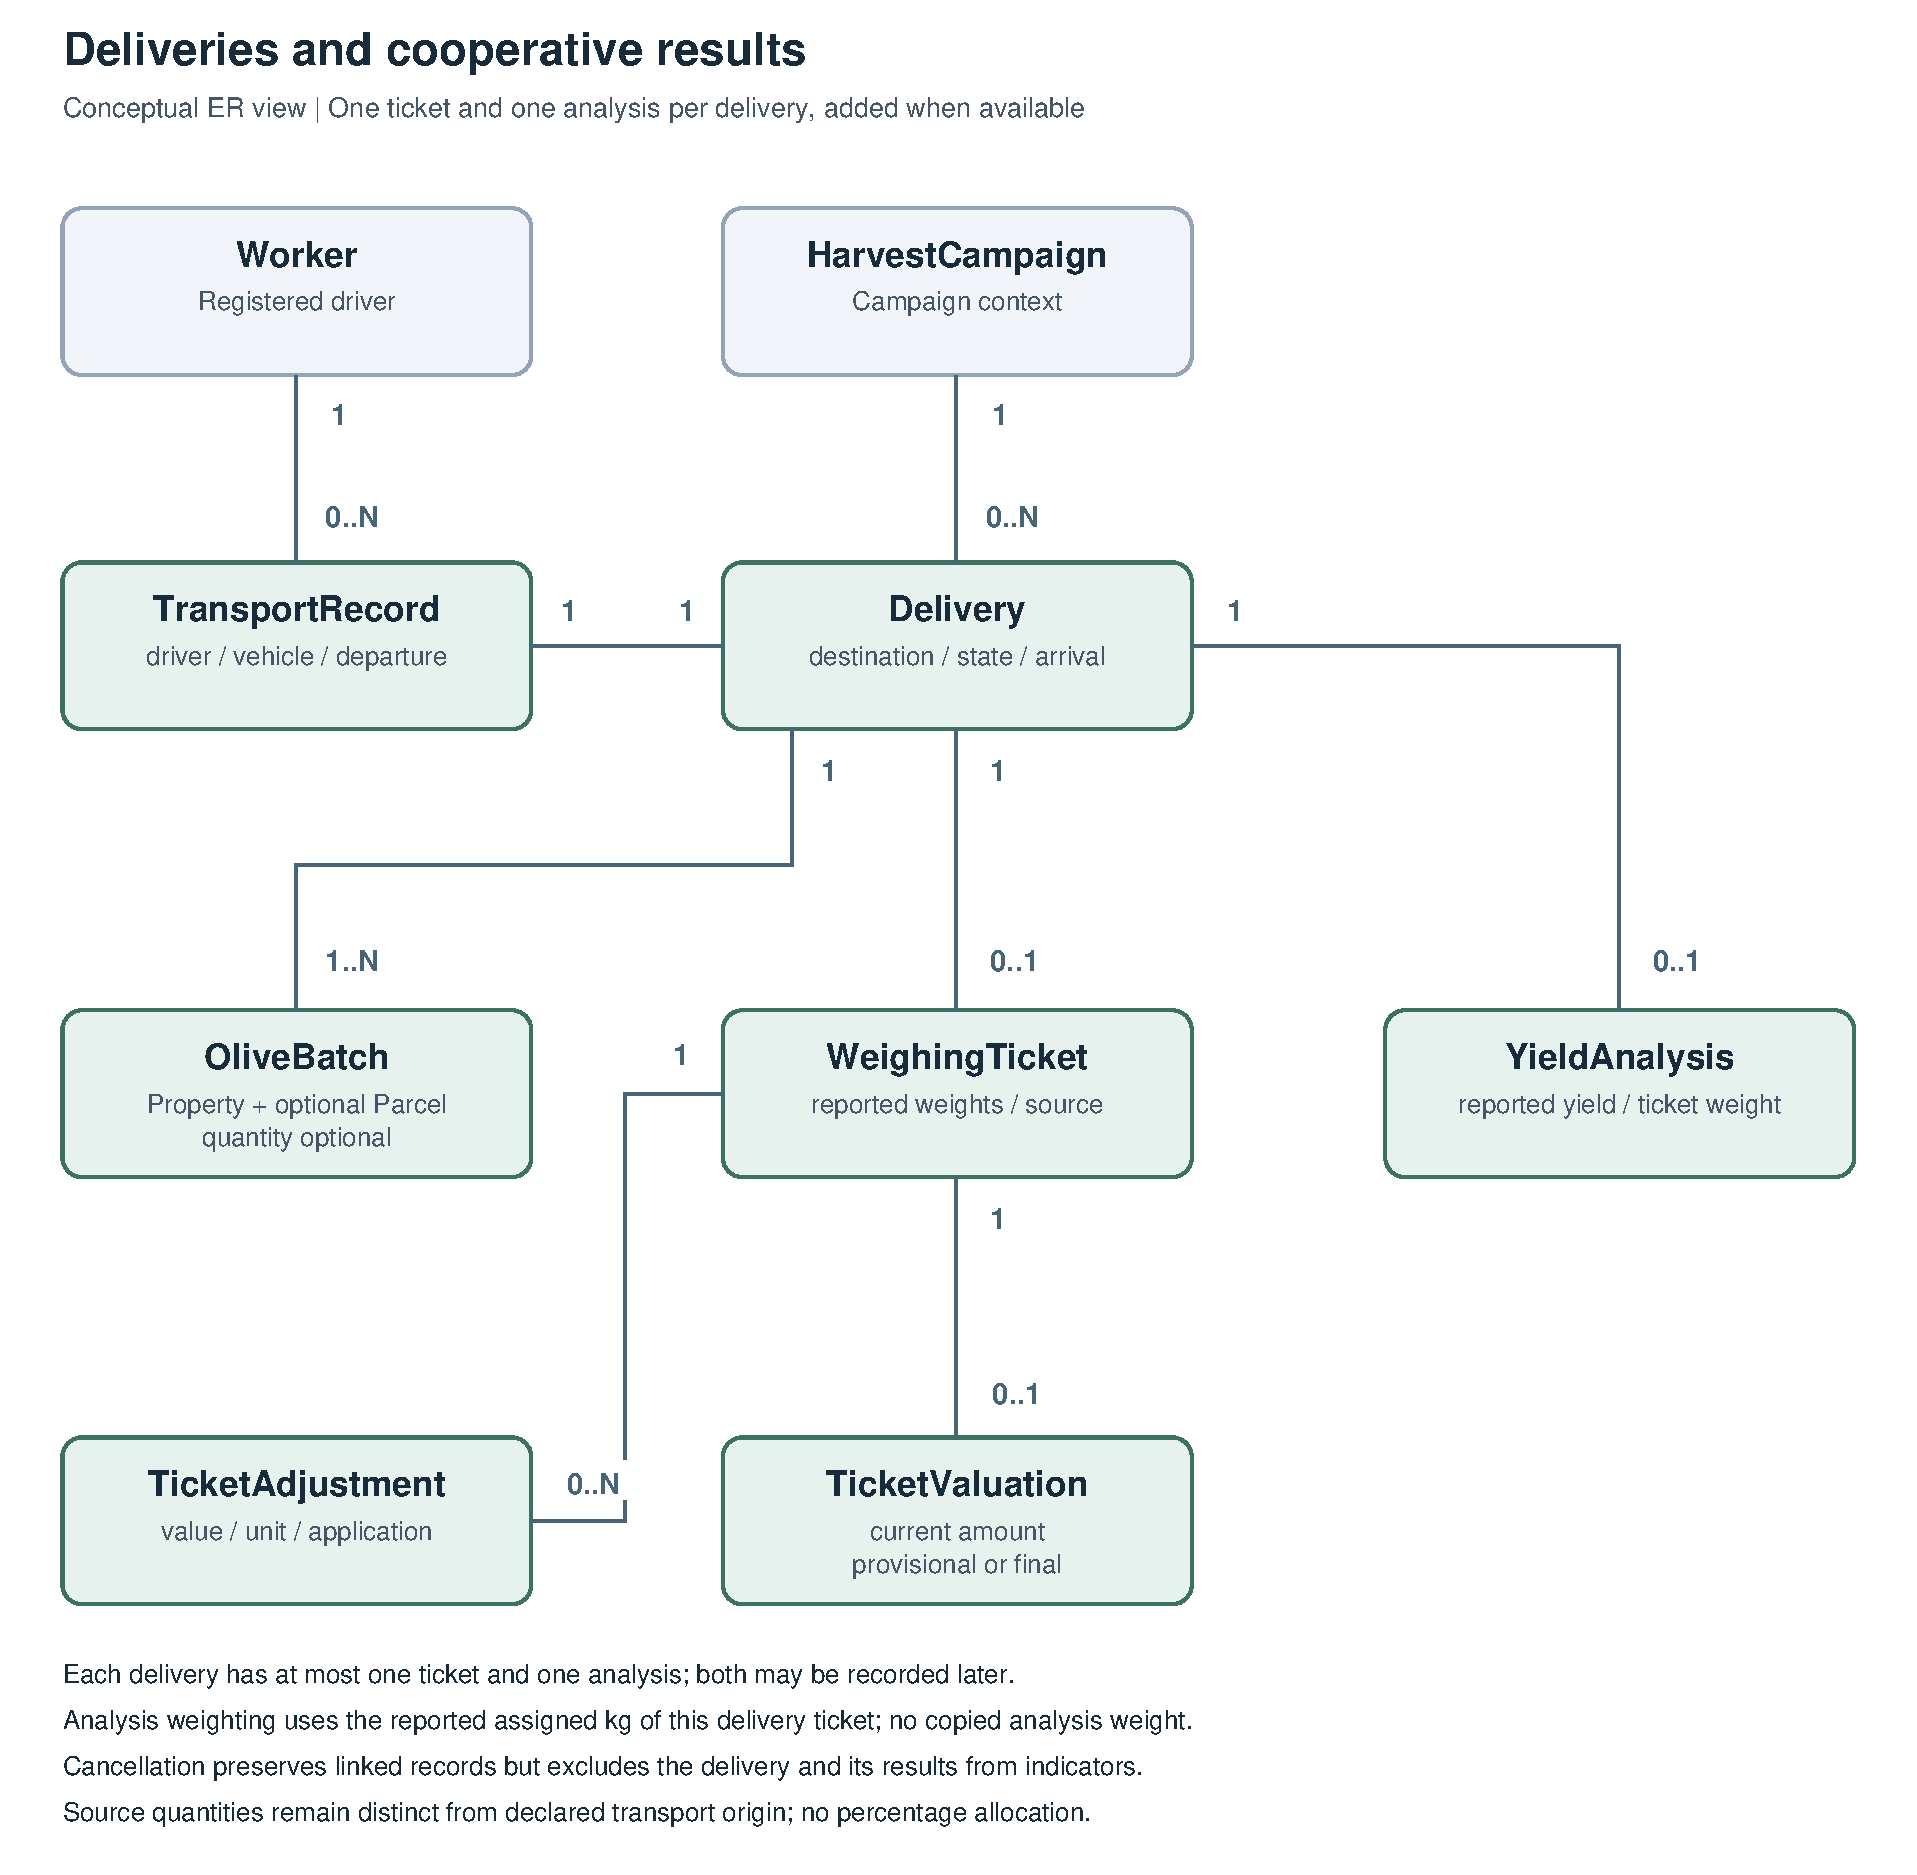
\includegraphics[width=\linewidth]{er-deliveries.pdf}
\caption{Each delivery has at most one ticket and one analysis. Source batches remain distinct from official weights.}
\label{fig:er-deliveries}
\end{figure}
WeighingTicket has a unique delivery reference and an optional canonical reported
accepted assigned weight in kg. Other weights retain source meanings/units. Optional
weighing start/end and reported excess duration are descriptive source facts.
TicketAdjustment also represents reported monetary penalties, protected by financial
grants; the application does not calculate or reapply them.
YieldAnalysis has a unique delivery reference and the reported yield percentage.
Its weighting reference is reached through the delivery's ticket; no independently
editable reference-weight copy is stored. TicketValuation is one current reported
amount per ticket. SourceAttachment supplies separate evidence links.
Source records may exist while Delivery is In transport. Indicator queries use
the Delivered, non-cancelled parent predicate in \hyperref[br:038]{\identifier{BR-038}}; source
existence alone does not confirm receipt.
The current model records known quantities in OliveBatch and one total amount
in TicketValuation; it has no field for monetary amounts by source. Mixed-load
amounts therefore remain unallocated by property/parcel, even when source quantities
are known. Supporting reported source amounts would require an explicit model
extension and review. No monetary allocation proportional to weight is inferred.
Delivery cancellation stores reason, time and actor while preserving dependent
records; lifecycle and correction behaviour follow \hyperref[br:031]{\identifier{BR-031}}.
Eligible hard deletion removes composed TransportRecord and OliveBatch rows in the
same validated operation, only when no ticket, analysis, valuation or evidence blocks it.

\paragraph{Ticket source fields.}
A validated source metadata snapshot holds source date/season, line, sample/member
references, quality/variety, municipality, literal POL/PAR/REC/PARAJE and locator
(Table~\ref{tab:source-ticket}). These source facts do not silently edit properties,
parcels, worker identities or transport records. Total kg and other source weights use validated reported-weight entries; KILOS ASIGNADOS uses only the typed canonical assigned kg field, which remains unknown if no accepted weight was reported. MEDIANERIA records the accepted percentage without generating a second assigned-weight value. Store printed
duration in seconds separately from start/end and excess time, with discrepancies
flagged for review. No penalty-calculation entity or integration is introduced.

\subsubsection{Worker Documents, Generation and Signatures}
Document has one required Worker reference and identifies category/title/subtype;
DocumentVersion holds that worker's accepted source and version-specific metadata.
WorkerSignature binds the document worker to one reviewed version and identifies
the initiating User separately. The worker signs, not the initiating account.
Figure~\ref{fig:er-documents} shows individual document sources and signing results.
\begin{figure}[!htbp]\centering
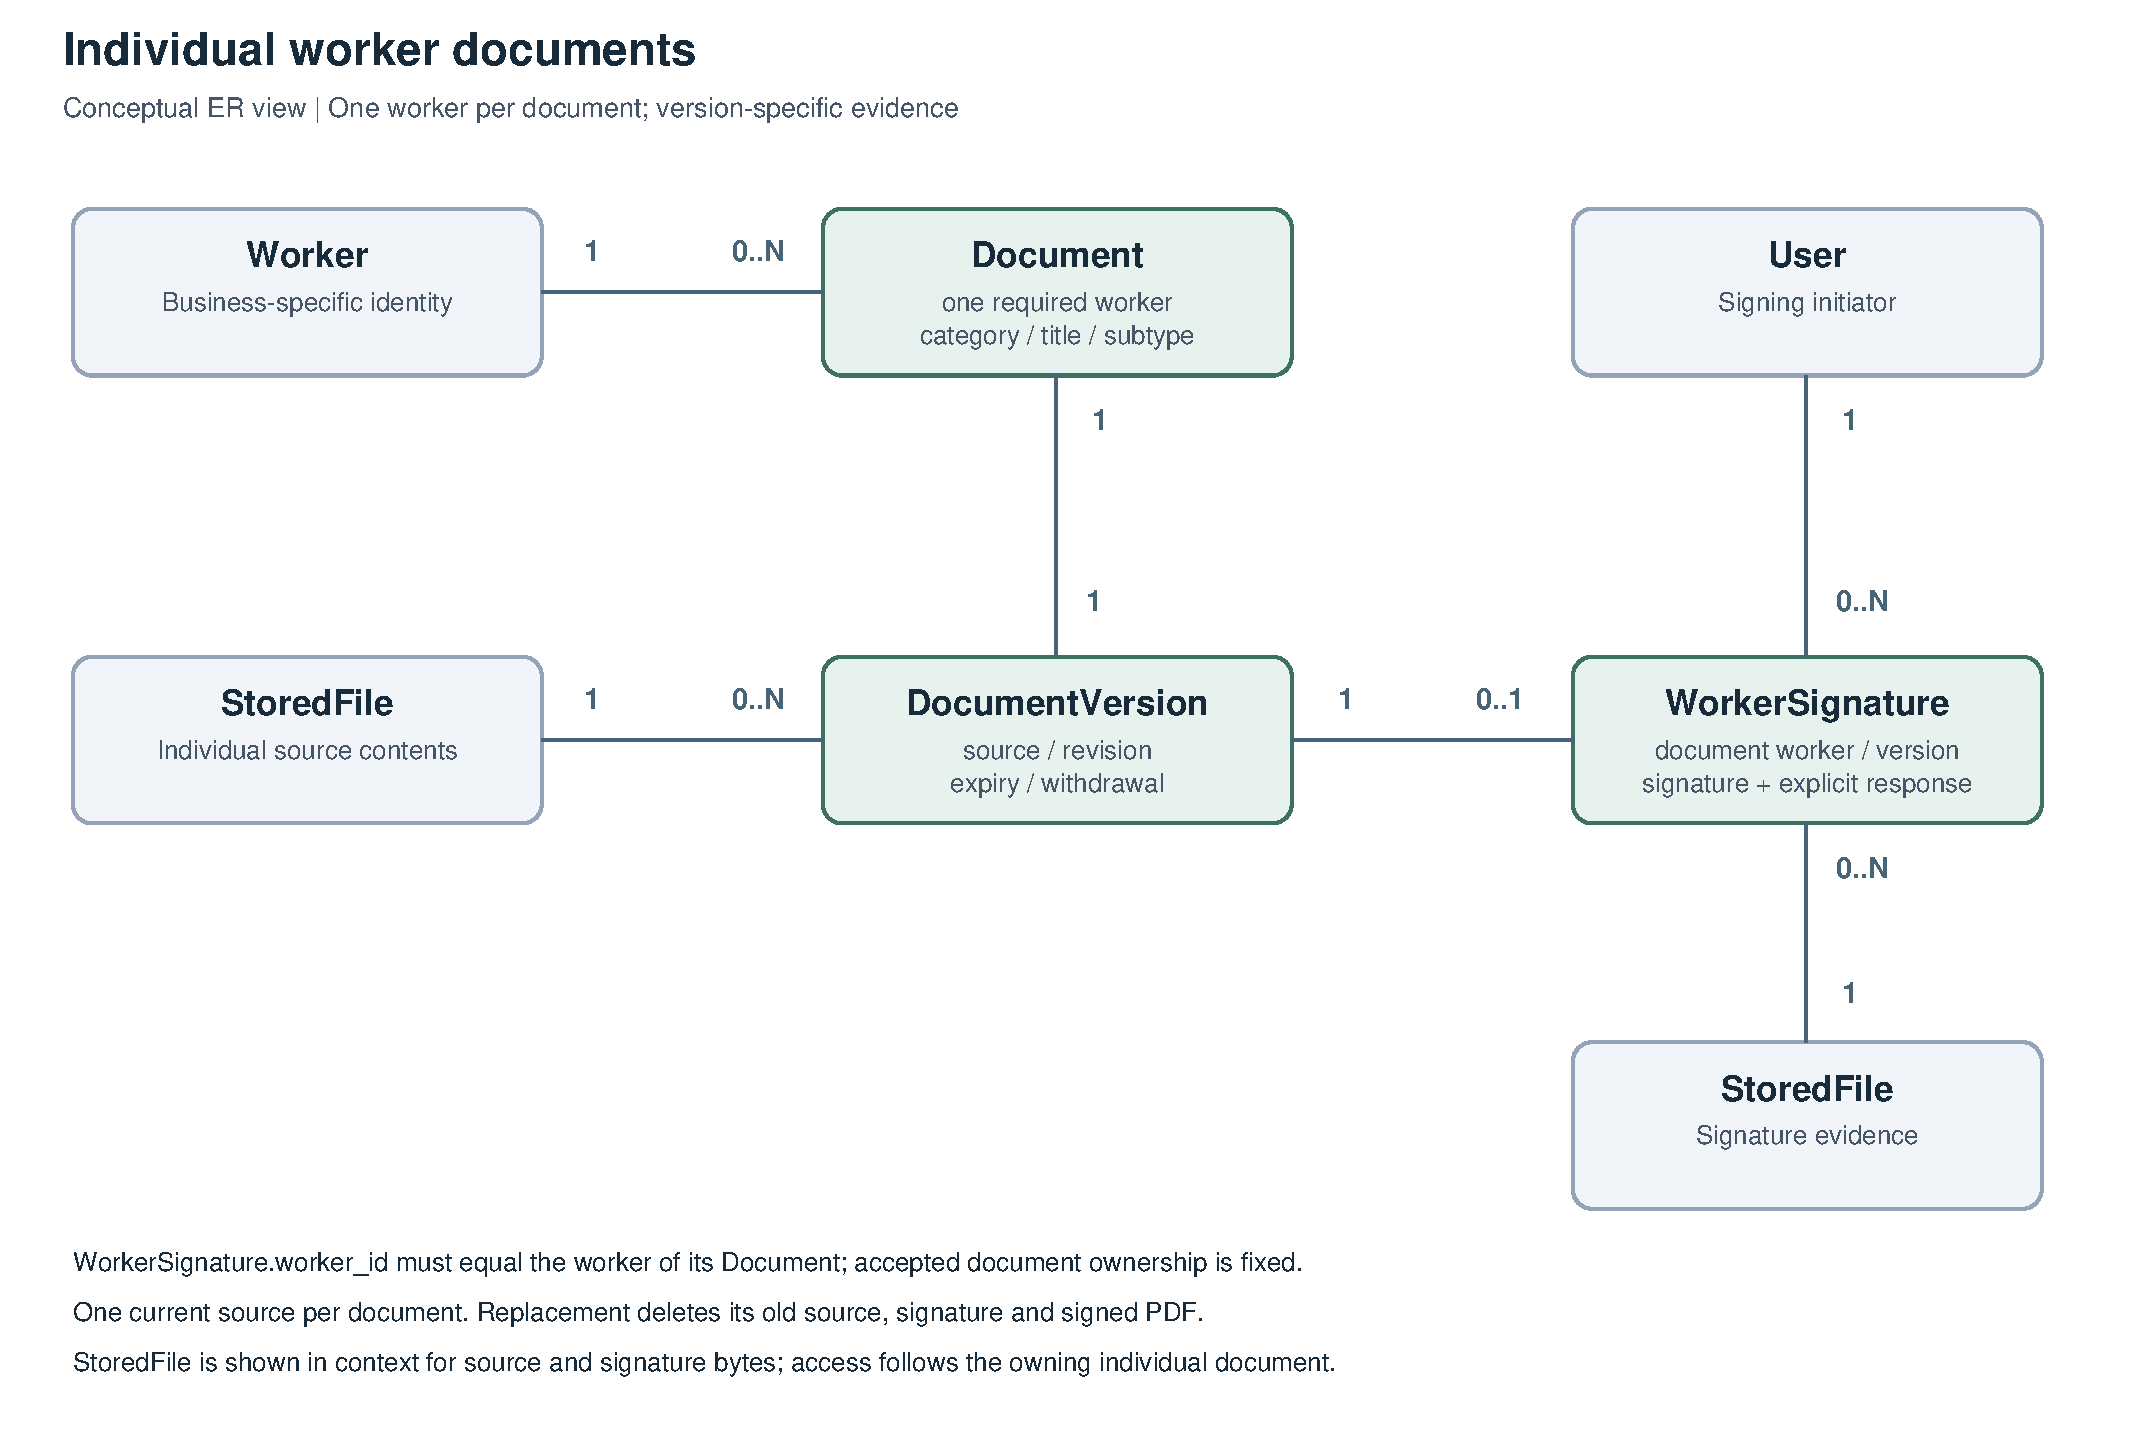
\includegraphics[width=\linewidth]{er-documents.pdf}
\caption{Individual sources and worker/version signing results. StoredFile is one entity shown in contextual views.}
\label{fig:er-documents}
\end{figure}
DocumentVersion separates source identity, currency, withdrawal, recorded expiry
and external-signature declaration. WorkerSignature records individual signing;
retention/cleanup follows \hyperref[br:026]{\identifier{BR-026}}, including deletion of a superseded source, signature and PDF and temporary recovery of ineligible signing proposals under \decisionref{Q-DOC-04}.

DocumentTemplate supplies an available model, category, revision and field schema.
Generated DocumentVersion records the template reference/revision and reviewed
input snapshot. Signing preserves that source and adds worker-specific evidence
and a derived signed PDF under \identifier{FR-042(d)}, for uploaded and generated versions alike.
DocumentRendition links a derived PDF to that version and worker. The worker-specific
rendition contains the document worker's captured signature and explicit response
where required, preserving source contents. Regeneration is not another signing event.
Figure~\ref{fig:er-generation} shows how generation and renditions relate to the source.
\begin{figure}[!htbp]\centering
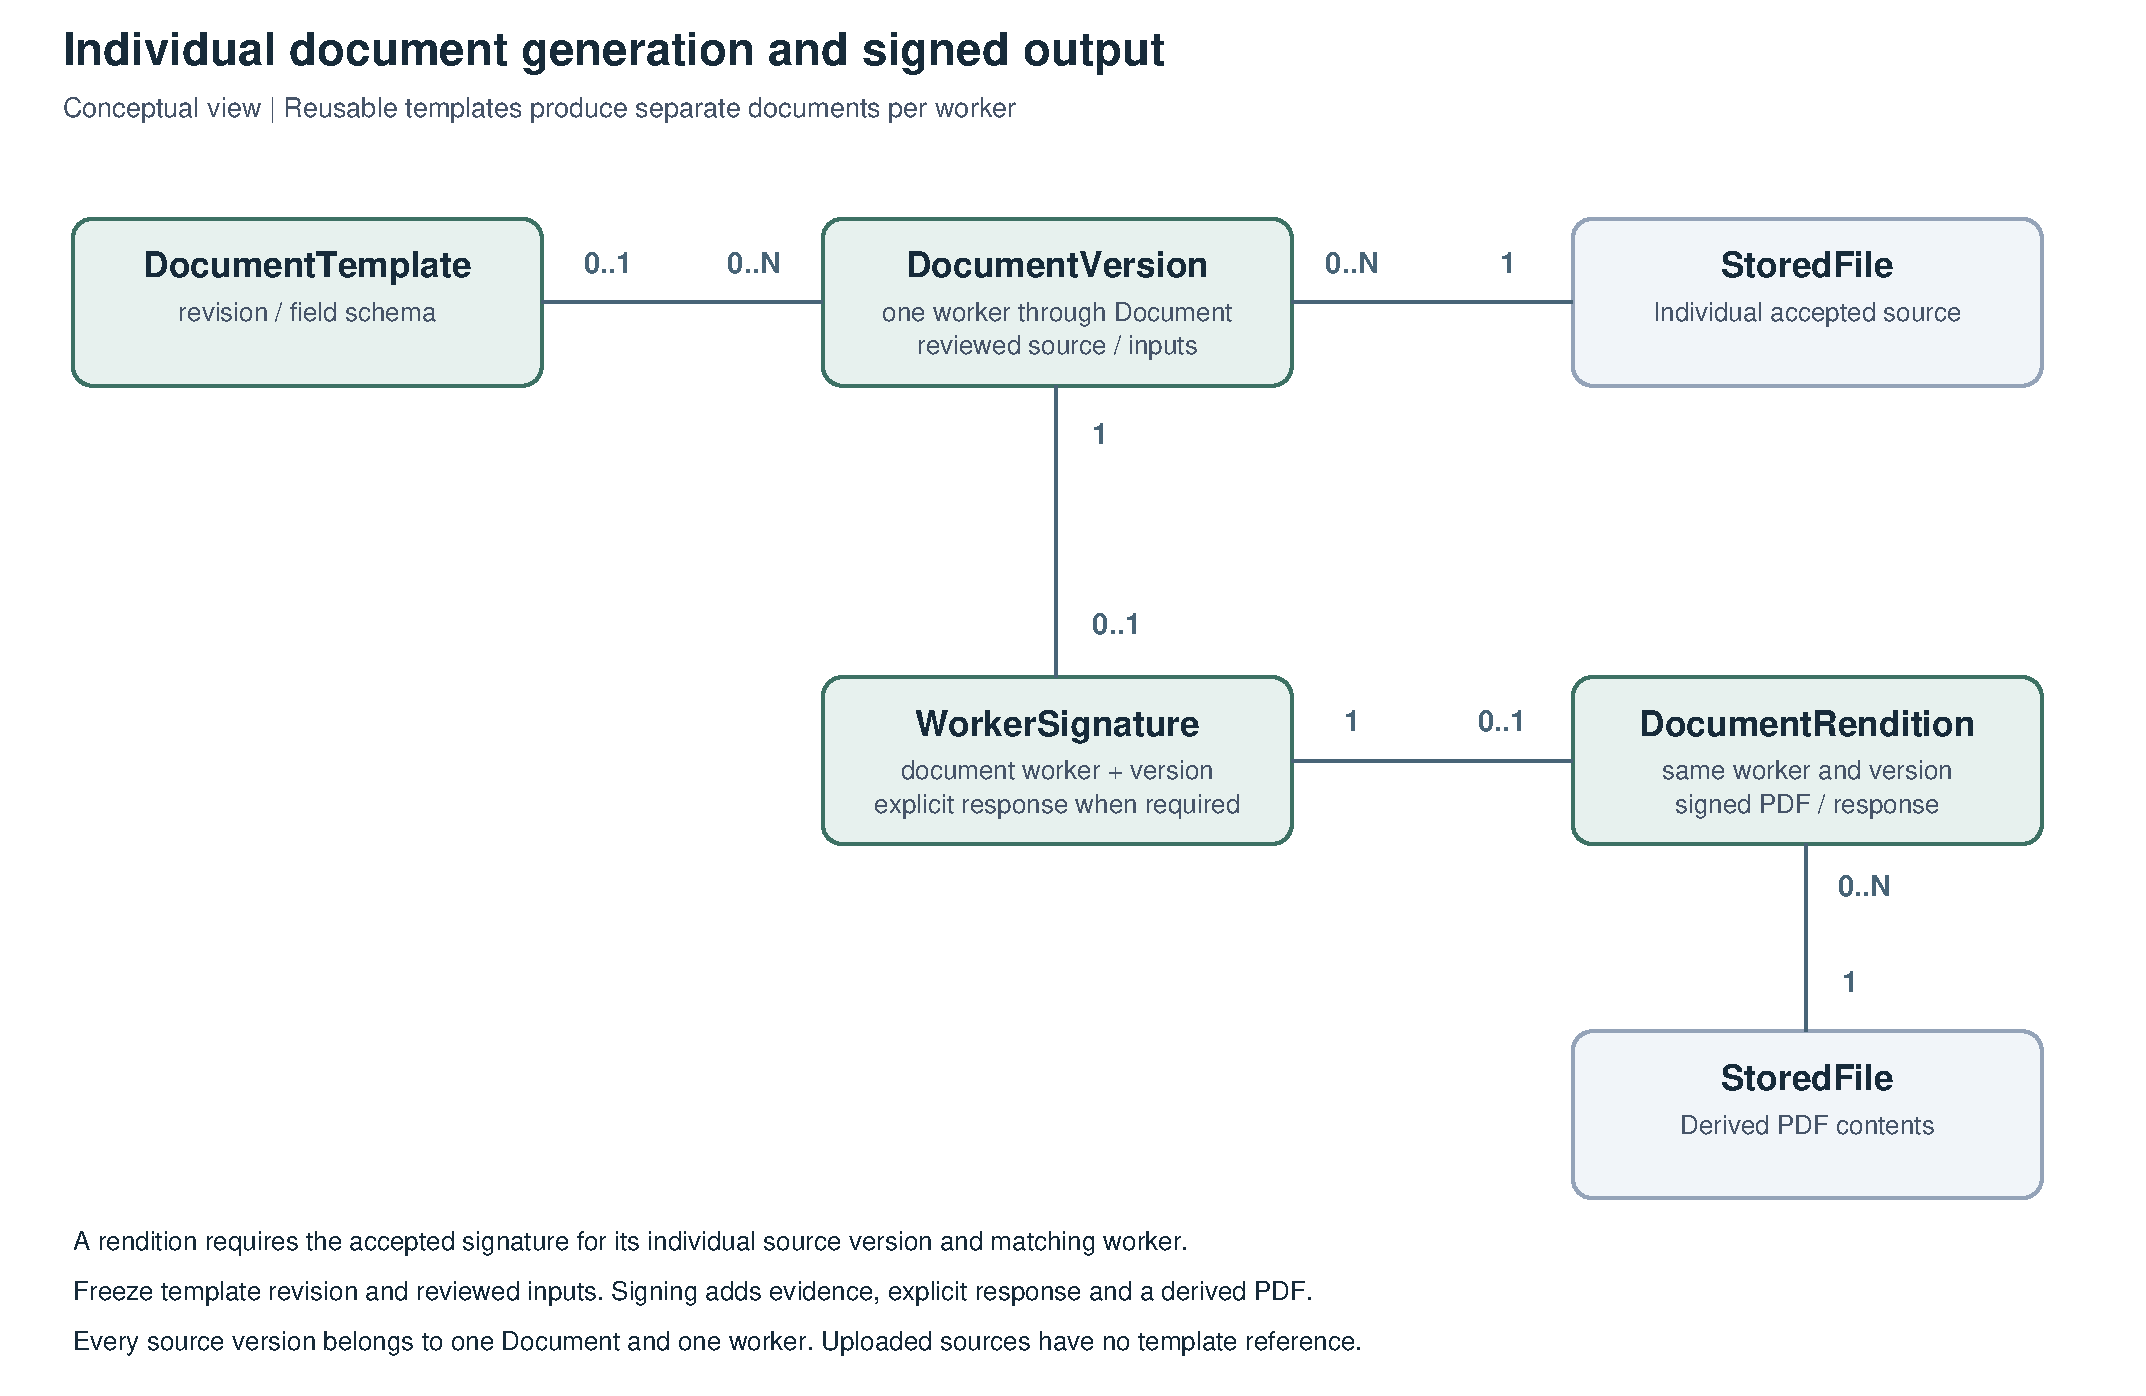
\includegraphics[width=\linewidth]{er-generation.pdf}
\caption{Template-based generation and worker-specific derived signed PDFs. Uploaded versions have no template reference.}
\label{fig:er-generation}
\end{figure}
The supplied inventory appears in Table~\ref{tab:source-forms}; the selected Spanish wording is preserved, with rendering and field mapping to be tested by the team. Document records subtype, DocumentVersion freezes source/template
inputs and any reviewed external response, and WorkerSignature binds an explicit
response to the signing event. Generation leaves consent undecided until signing;
evidence/PDF preserves the decision. Every document has one worker and one current accepted source. Replacement deletes the previous source, signature and PDF without a consultable history. Reusing a
template creates independent documents for each selected worker. Identity/permit originals are uploaded evidence; generation does not issue
them. Worker activity is derived in the profile under \identifier{FR-023}, without a dedicated attendance-document workflow. Source generation/acceptance
requires connectivity, while an accepted prepared version may be signed offline.

\subsubsection{Stored Files and Source Evidence}
\label{sec:conceptual-files}
StoredFile holds storage metadata shared by document contents, captured signatures
and source evidence. SourceAttachment links one stored file to exactly one ticket,
analysis or valuation; the three target relationships are exclusive alternatives.
This keeps source evidence independent of worker-document version retention.
Figure~\ref{fig:er-source-files} shows the exclusive attachment targets.

File access is authorised through the associated business record, never the storage
key alone. There is no global deduplication or cross-workspace reuse. Remove content
only after releasing retained references. An explicit attachment replacement keeps the old file until the new file is fully stored and validated, then switches the reference and deletes the previous file without history under \decisionref{Q-AT-02}. Failed uploads preserve the old evidence. Prepared-file protection remains under
\decisionref{Q-DOC-07}.

Apply the complete-file consultation and upload grants in
Section~\ref{sec:permission-defaults}. A complete ticket may expose printed monetary
values; consultation grants must therefore be configured consistently. Changing or
removing a link cannot grant another account access to its file. Worker-document
upload remains a separate operation.

\begin{figure}[!htbp]
\centering
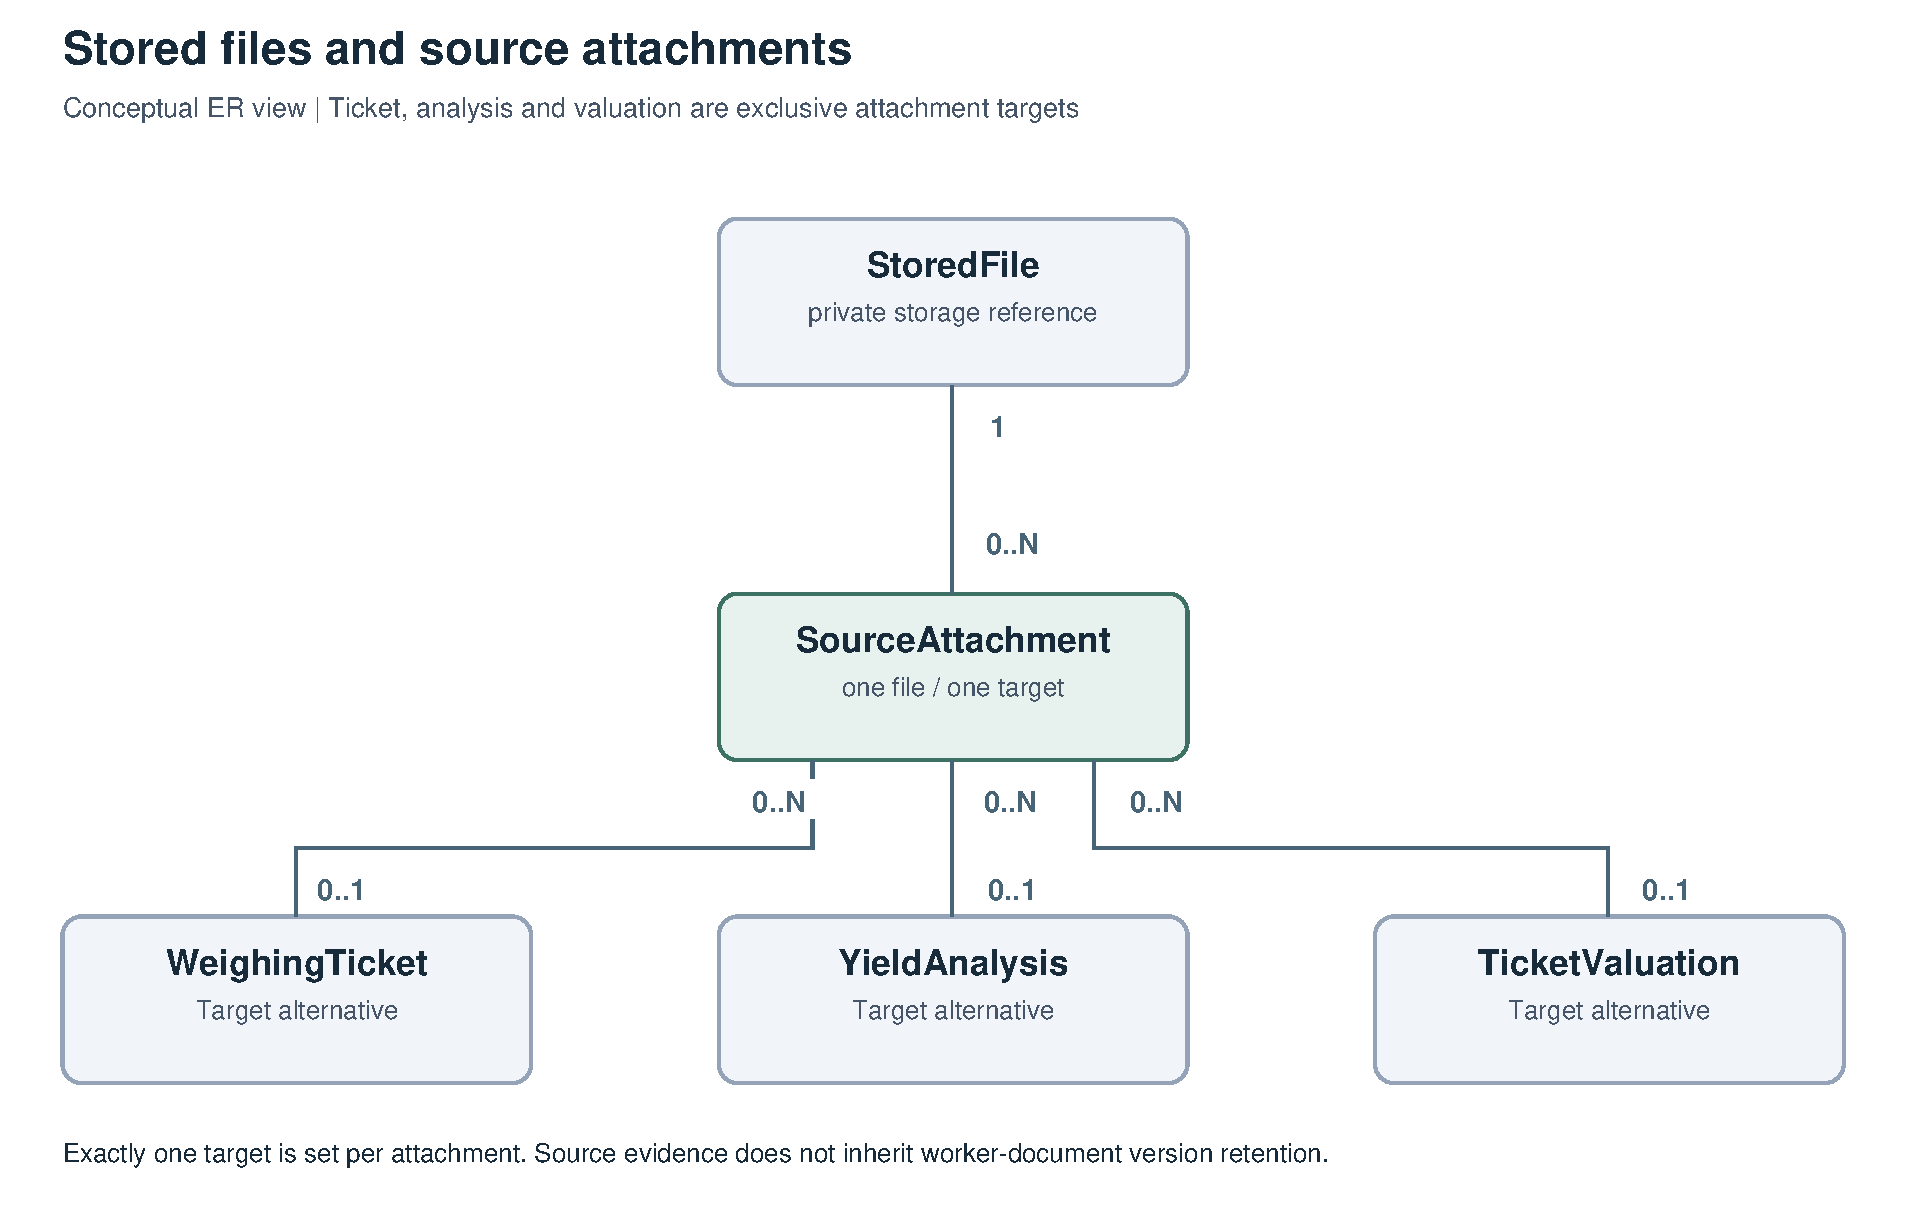
\includegraphics[width=\textwidth]{figures/er-source-files.pdf}
\caption{Source attachments and stored content. Each attachment targets exactly one source record; the three target links are exclusive alternatives.}
\label{fig:er-source-files}
\end{figure}

\FloatBarrier
\Needspace{10\baselineskip}
\subsection{Logical Data Model}
\label{sec:data-logical}
\paragraph{Conventions.}
Each table has a stable UUID id. Business-scoped tables carry workspace identity;
parent, worker, area and file references must stay in that workspace. Shared server
metadata comprises creation/update times, author where relevant and a revision
counter for concurrency, not a full field-change history. Accepted records satisfy
requiredness; a locally pending proposal is not central acceptance.
Optional parcel means whole-property scope; area uniqueness must handle NULL
explicitly. The table lists principal fields, not the full dictionary. Work timestamps are complete UTC instants with capture-time IANA timezone metadata. Device timezone drives entry/display; the initially device-suggested and owner-confirmed business timezone determines the shared start-based working date.
{\readabletable
\begin{longtable}{L{0.27}L{0.4}L{0.33}}
\caption{Principal entities, fields and relationships in the logical data model.}\label{tab:logical-model}\\
\toprule\rowcolor{TableHeader}
\textbf{Entity / table} & \textbf{Principal fields} & \textbf{Relationships / key} \\
\midrule\endfirsthead
\toprule\rowcolor{TableHeader}
\textbf{Entity / table} & \textbf{Principal fields} & \textbf{Relationships / key} \\
\midrule\endhead
\multicolumn{3}{r}{\footnotesize\itshape Continued on next page}\\\endfoot
\bottomrule\endlastfoot
User\newline \texttt{app\_\allowbreak{}user} & \mbox{\texttt{name}}, \mbox{\texttt{normalised\_email}}, \mbox{\texttt{account\_status}}, \mbox{\texttt{system\_role}}, \mbox{\texttt{provisioned\_by\_admin\_id}} & Global identity; unique normalised email. Verified changes preserve id. \\
\midrule
Workspace\newline \texttt{workspace} & \mbox{\texttt{name}}, \mbox{\texttt{business\_timezone}}, \mbox{\texttt{status}} & Single client workspace, pending until owner activation; timezone suggested from the creating device and explicitly confirmed; Owner through membership. \\
\midrule
WorkspaceMembership\newline \texttt{workspace\_\allowbreak{}membership} & \mbox{\texttt{user\_id}}, \mbox{\texttt{workspace\_role}}, \mbox{\texttt{access\_status}}, \mbox{\texttt{revoked\_at}} & User; unique workspace/User pair. \\
\midrule
ManagerInvitation\newline \texttt{manager\_\allowbreak{}invitation} & \mbox{\texttt{recipient\_email}}, \mbox{\texttt{invited\_by\_user\_id}}, \mbox{\texttt{invitation\_status}}, \mbox{\texttt{expires\_at}} & Intended verified recipient; issuer and accepted membership. \\
\midrule
AccessGrant\newline \texttt{access\_\allowbreak{}grant} & \mbox{\texttt{membership\_id}}, \mbox{\texttt{operation\_code}}, \mbox{\texttt{property\_id}} & Required property scope; parcels/current/future campaigns inherit it. Unique membership/operation/property; insurance constraint. \\
\midrule
WorkerAvailability\newline \texttt{worker\_\allowbreak{}availability} & \mbox{\texttt{membership\_id}}, \mbox{\texttt{worker\_id}} & Owner-explicit worker availability; unique membership/worker, same workspace; no other-property work authority. \\
\midrule
Property\newline \texttt{property} & \mbox{\texttt{name}}, \mbox{\texttt{textual\_location}}, \mbox{\texttt{declared\_area\_ha}}, \mbox{\texttt{olive\_varieties}} & Workspace; parent of Parcels. \\
\midrule
Parcel\newline \texttt{parcel} & \mbox{\texttt{property\_id}}, \mbox{\texttt{name}}, \mbox{\texttt{declared\_area\_ha}}, \mbox{\texttt{olive\_varieties}} & Property in the same workspace. \\
\midrule
HarvestCampaign\newline \texttt{harvest\_\allowbreak{}campaign} & \mbox{\texttt{name}}, \mbox{\texttt{planned\_start\_date}}, \mbox{\texttt{actual\_start\_date}}, \mbox{\texttt{actual\_end\_date}}, \mbox{\texttt{lifecycle\_status}} & Workspace; Planned/In progress/Closed; one or more coverage entries. \\
\midrule
CampaignCoverage\newline \texttt{campaign\_\allowbreak{}coverage} & \mbox{\texttt{campaign\_id}}, \mbox{\texttt{property\_id}}, \mbox{\texttt{parcel\_id}} & Campaign, Property, optional Parcel; unique selected area. \\
\midrule
Worker\newline \texttt{worker} & \mbox{\texttt{full\_name}}, \mbox{\texttt{telephone}}, \mbox{\texttt{official\_id\_type}}, \mbox{\texttt{official\_id\_country}}, \mbox{\texttt{official\_id\_number}}, \mbox{\texttt{can\_operate\_machinery}}, \mbox{\texttt{capability\_description}} & Workspace; no required User FK. \\
\midrule
WorkPlan\newline \texttt{work\_\allowbreak{}plan} & \mbox{\texttt{campaign\_id}}, \mbox{\texttt{work\_date}} & Campaign; unique campaign/date. \\
\midrule
PlannedAssignment\newline \texttt{planned\_\allowbreak{}assignment} & \mbox{\texttt{plan\_id}}, \mbox{\texttt{worker\_id}}, \mbox{\texttt{property\_id}}, \mbox{\texttt{parcel\_id}} & Plan, Worker, area; unique plan/worker/area. \\
\midrule
PlannedWorkPeriod\newline \texttt{planned\_\allowbreak{}work\_\allowbreak{}period} & \mbox{\texttt{assignment\_id}}, \mbox{\texttt{worker\_id}}, \mbox{\texttt{planned\_start}}, \mbox{\texttt{planned\_end}} & PlannedAssignment; checked worker reference. \\
\midrule
PlannedBreak\newline \texttt{planned\_\allowbreak{}break} & \mbox{\texttt{assignment\_id}}, \mbox{\texttt{break\_start}}, \mbox{\texttt{break\_end}}, \mbox{\texttt{counts\_as\_work}} & PlannedAssignment. \\
\midrule
DailyAttendance\newline \texttt{daily\_\allowbreak{}attendance} & \mbox{\texttt{worker\_id}}, \mbox{\texttt{work\_date}}, \mbox{\texttt{attendance\_status}} & Worker; unique workspace/worker/date. \\
\midrule
ActualWorkAssignment\newline \texttt{actual\_\allowbreak{}work\_\allowbreak{}assignment} & \mbox{\texttt{attendance\_id}}, \mbox{\texttt{worker\_id}}, \mbox{\texttt{campaign\_id}}, \mbox{\texttt{property\_id}} & Attendance, Campaign, area; optional source plan assignment. Unique attendance/campaign/area. \\
\midrule
WorkPeriod\newline \texttt{work\_\allowbreak{}period} & \mbox{\texttt{assignment\_id}}, \mbox{\texttt{worker\_id}}, \mbox{\texttt{actual\_start}}, \mbox{\texttt{actual\_end}}, \mbox{\texttt{task\_code}} & ActualWorkAssignment; the worker reference must match the associated actual assignment. \\
\midrule
WorkBreak\newline \texttt{work\_\allowbreak{}break} & \mbox{\texttt{attendance\_id}}, \mbox{\texttt{break\_start}}, \mbox{\texttt{break\_end}}, \mbox{\texttt{counts\_as\_work}} & DailyAttendance. \\
\midrule
Delivery\newline \texttt{delivery} & \mbox{\texttt{campaign\_id}}, \mbox{\texttt{destination\_name}}, \mbox{\texttt{delivery\_status}}, \mbox{\texttt{delivered\_at}}, \mbox{\texttt{cancellation\_reason}} & Campaign; one transport and one or more source batches; cancellation preserves dependants. \\
\midrule
TransportRecord\newline \texttt{transport\_\allowbreak{}record} & \mbox{\texttt{delivery\_id}}, \mbox{\texttt{driver\_worker\_id}}, \mbox{\texttt{vehicle\_reference}}, \mbox{\texttt{departure\_at}}, \mbox{\texttt{transport\_document\_reference}}, \mbox{\texttt{declared\_origin\_property\_id}}, \mbox{\texttt{declared\_origin\_parcel\_id}} & Unique Delivery; Worker driver. Declared origin is separate from OliveBatch. \\
\midrule
OliveBatch\newline \texttt{olive\_\allowbreak{}batch} & \mbox{\texttt{delivery\_id}}, \mbox{\texttt{property\_id}}, \mbox{\texttt{parcel\_id}}, \mbox{\texttt{collection\_origin}} & Delivery; source area within campaign coverage. \\
\midrule
WeighingTicket\newline \texttt{weighing\_\allowbreak{}ticket} & \mbox{\texttt{delivery\_id}}, \mbox{\texttt{assigned\_weight\_kg}}, \mbox{\texttt{reported\_weights}}, \mbox{\texttt{source\_metadata}}, \mbox{\texttt{source\_date}}, \mbox{\texttt{reported\_duration\_seconds}}, \mbox{\texttt{weighing\_started\_at}}, \mbox{\texttt{weighing\_ended\_at}}, \mbox{\texttt{excess\_time\_value}}, \mbox{\texttt{excess\_time\_unit}} & Unique delivery; canonical reported accepted assigned kg plus optional source timing. \\
\midrule
TicketAdjustment\newline \texttt{ticket\_\allowbreak{}adjustment} & \mbox{\texttt{ticket\_id}}, \mbox{\texttt{adjustment\_type}}, \mbox{\texttt{reported\_value}}, \mbox{\texttt{unit}} & WeighingTicket. \\
\midrule
YieldAnalysis\newline \texttt{yield\_\allowbreak{}analysis} & \mbox{\texttt{delivery\_id}}, \mbox{\texttt{yield\_percentage}}, \mbox{\texttt{analysis\_date}} & Unique delivery. Weight through that delivery's ticket; no copied reference weight. \\
\midrule
TicketValuation\newline \texttt{ticket\_\allowbreak{}valuation} & \mbox{\texttt{ticket\_id}}, \mbox{\texttt{amount}}, \mbox{\texttt{currency}}, \mbox{\texttt{valuation\_status}} & Unique WeighingTicket; current value only. \\
\midrule
Document\newline \texttt{document} & \mbox{\texttt{title}}, \mbox{\texttt{document\_category}}, \mbox{\texttt{form\_type}}, \mbox{\texttt{worker\_id}} & One required Worker; one current accepted source, without consultable history. \\
\midrule
DocumentVersion\newline \texttt{document\_\allowbreak{}version} & \mbox{\texttt{document\_id}}, \mbox{\texttt{version\_number}}, \mbox{\texttt{source\_file\_id}}, \mbox{\texttt{origin\_kind}}, \mbox{\texttt{template\_id}}, \mbox{\texttt{template\_revision}}, \mbox{\texttt{is\_withdrawn}} & Unique document reference: one current accepted source. New identity/sequence on replacement; superseded source, signature and PDF deleted. \\
\midrule
WorkerSignature\newline \texttt{worker\_\allowbreak{}signature} & \mbox{\texttt{worker\_id}}, \mbox{\texttt{version\_id}}, \mbox{\texttt{initiated\_by\_user\_id}}, \mbox{\texttt{client\_signed\_at}}, \mbox{\texttt{form\_response}} & Worker, Version, User, StoredFile; unique worker/version; worker must equal Document.worker\_id. \\
\midrule
StoredFile\newline \texttt{stored\_\allowbreak{}file} & \mbox{\texttt{storage\_key}}, \mbox{\texttt{original\_filename}}, \mbox{\texttt{media\_type}}, \mbox{\texttt{byte\_size}} & Private content; unique storage key. \\
\midrule
SourceAttachment\newline \texttt{source\_\allowbreak{}attachment} & \mbox{\texttt{stored\_file\_id}}, \mbox{\texttt{ticket\_id}}, \mbox{\texttt{analysis\_id}}, \mbox{\texttt{valuation\_id}} & StoredFile; exactly one populated target FK. \\
\midrule
DocumentTemplate\newline \texttt{document\_\allowbreak{}template} & \mbox{\texttt{name}}, \mbox{\texttt{document\_category}}, \mbox{\texttt{template\_file\_id}}, \mbox{\texttt{revision}}, \mbox{\texttt{field\_schema}} & Workspace; template StoredFile and reviewed field schema. \\
\midrule
DocumentRendition\newline \texttt{document\_\allowbreak{}rendition} & \mbox{\texttt{version\_id}}, \mbox{\texttt{worker\_id}}, \mbox{\texttt{stored\_file\_id}}, \mbox{\texttt{generated\_at}} & Unique version/worker; derived PDF StoredFile; associated accepted signature; worker matches Document. \\
\end{longtable}}

Other ticket weights and template/invitation/input schemas use validated JSON;
core relationships remain foreign keys. Assigned kg is a canonical typed ticket column populated from KILOS ASIGNADOS, not duplicated in JSON or analysis. A monetary penalty is a reported
TicketAdjustment with EUR unit and known application status. Unique delivery
references enforce one ticket and one analysis even under concurrent requests.
The selected Spanish template/revision and input snapshot freeze the current generated source context;
the rendition never replaces that source. Repeated rendering does not create
another worker/version signature.

\Needspace{9\baselineskip}
\subsection{Data Dictionary}
\label{sec:data-dictionary}
The complete current field inventory is maintained separately in
\nolinkurl{technical/data-architecture/data-dictionary.tex}. The following meanings
are essential to interpreting the condensed model.
{\readabletable
\begin{longtable}{L{0.31}L{0.69}}
\caption{Key field groups and their meanings.}\label{tab:data-dictionary-summary}\\
\toprule\rowcolor{TableHeader}
\textbf{Field group} & \textbf{Meaning} \\
\midrule\endfirsthead
\toprule\rowcolor{TableHeader}
\textbf{Field group} & \textbf{Meaning} \\
\midrule\endhead
\multicolumn{2}{r}{\footnotesize\itshape Continued on next page}\\\endfoot
\bottomrule\endlastfoot
Identity and scope & User identifies an account; Worker identifies a person within a business, using a separate UUID. Required worker fields: full name, telephone and official identification type/country/number. Workspace references and composite keys prevent cross-business links. \\
\midrule
Dates and timezone & Confirmed business timezone governs daily grouping; device timezone drives entry/display with preserved capture context. Full instants preserve overnight and clock-change meaning. Enter minutes; report hours/minutes. Entry, event and acceptance times differ. Only selected/expected workers await attendance; complete confirmed periods require a task. \\
\midrule
Delivery state & In transport, delivered or cancelled. Campaign lifecycle is separately Planned, In progress or Closed. Cancellation has reason/actor/time, preserves source records and excludes their contributions. \\
\midrule
Reported weights & assigned\_weight\_kg is the ticket's canonical cooperative-reported accepted assigned kg. Other weights preserve meanings/units. Unknown is NULL, not zero. \\
\midrule
Yield reference & yield\_percentage is the reported result. Its weighted-average reference is read through the delivery ticket, not stored again on the analysis. \\
\midrule
Weighing and penalties & Start/end and excess duration/unit reproduce the ticket. Monetary penalties are reported adjustments; no scale-rate calculation or second deduction follows. \\
\midrule
Load provenance & OliveBatch stores actual origins and known quantities separately from declared transport origin. It has no source monetary amounts; mixed-load money remains unallocated by area. No proportional or dominant-parcel allocation is inferred. \\
\midrule
Version protection & Keep only the current document source until successful replacement, then delete the old source, signature and PDF for every category. No consultable history; pending old-source signing is ineligible and follows \identifier{Q-DOC-04} recovery. \\
\midrule
Generation and renditions & Template/revision and reviewed input snapshot identify generated sources. A rendition is a worker-specific derived signed PDF linked to its source version. \\
\midrule
Financial/local state & Reported provisional/final status is distinct from pending/accepted synchronisation. Offline financial content requires financial authorisation. \\
\midrule
Files & PDF/JPG/PNG uploads have the 10~MB limit. Availability/upload state does not prove server acceptance of dependent records. \\
\end{longtable}}

\paragraph{Source integrity.}
An accepted document source has a protected \texttt{content\_hash} under \identifier{SEC-08};
the full dictionary records the conditional requiredness by file purpose. This is
integrity metadata, not signer authentication or a replacement for version identity.

\paragraph{Operational source fields.}
The full reference records client-confirmed total/assigned-weight semantics, accepted percentage and independently printed duration.
Document subtype identifies the form; reviewed inputs are version snapshots. A
required acceptance/refusal choice is bound to signature evidence and rendered in
the appropriate form area. Signed, server-accepted and consent accepted are separate.

\paragraph{Technical account authority.}
User.system\_role distinguishes standard users from the Technical Administrator;
provisioned\_by\_admin\_id records the initial owner's issuer. It does not grant
access to agricultural records/files. Workspace and initial owner membership
remain pending until recipient activation; the complete field reference specifies
these additions within the existing 33-entity model.

\subsection{Integrity Constraints}
\label{sec:data-integrity}
Identity and row-level checks are insufficient for cross-record invariants. Enforce
the following at central transactional acceptance, including concurrent requests.
{\readabletable
\begin{longtable}{L{0.24}L{0.59}L{0.17}}
\caption{Cross-record integrity constraints.}\label{tab:integrity-constraints}\\
\toprule\rowcolor{TableHeader}
\textbf{Scope} & \textbf{Essential constraint} & \textbf{Rules} \\
\midrule\endfirsthead
\toprule\rowcolor{TableHeader}
\textbf{Scope} & \textbf{Essential constraint} & \textbf{Rules} \\
\midrule\endhead
\multicolumn{3}{r}{\footnotesize\itshape Continued on next page}\\\endfoot
\bottomrule\endlastfoot
Ownership/access & One owner per active workspace; all business parent/file links in scope. Apply owner-reviewed grants and mandatory insurance access. & \identifier{BR-001}--BR-004 \\
\midrule
Coverage/work & Parcel belongs to property; assignments fit coverage. Preserve unique attendance and non-overlapping same-worker planned/actual intervals, checked separately. Reopening precedes confirmed changes where required. & \identifier{BR-005}--BR-021 \\
\midrule
Delivery/results & Accepted delivery has transport and source batch(es). Unique delivery FK on ticket and analysis. Analysis weighting reads the same delivery ticket. Cancelled parents accept no new source results. & \identifier{BR-031}--BR-033 \\
\midrule
Corrections and cancellation & Validate affected campaign scopes, chronology, coverage and dependent data; no cascade deletion. Cancellation preserves sources and removes contributions. Hard deletion requires no dependent tickets, analyses, valuations or evidence; remove composed
transport/batch rows together. & \identifier{BR-031}, \identifier{BR-038} \\
\midrule
Values/evidence & One current valuation per ticket. Exactly one target per source attachment; combine all applicable association and complete-file consultation permissions, without mandatory monetary-content classification or automatic redaction. & \identifier{BR-024}, \identifier{BR-034}--BR-036 \\
\midrule
Versions/signatures & Unique document/version sequence and accepted worker/version signature. Signer must equal the document's single Worker reference. One current accepted source per document. Successful replacement deletes the old source, signature and PDF, even when signed; invalidate old-source signing without transferring or recreating it. Temporary local proposal recovery follows \identifier{Q-DOC-04}, not a version-history policy. & \identifier{BR-023}--BR-030 \\
\midrule
Generation/rendition & Generated source has reviewed template/revision/input snapshot; accepted rendition uses associated worker/version signature and same-workspace files. Source identity remains immutable. & \identifier{BR-041} \\
\midrule
Files/acceptance & Apply upload format/limit checks. No current source before file readiness. Revision/idempotency checks prevent duplicate effects; cleanup respects all retained references. & \identifier{BR-021}, \identifier{BR-044} \\
\end{longtable}}

Coverage reservation, intervals, sequence allocation and minimum-child counts need
transactional enforcement. File cleanup is recoverable across database/object-store
boundaries. The team verifies replacement file cleanup, positive/non-overlapping break validation, out-of-period warnings and recovery mechanisms against the approved NFRs.


Planned campaigns may overlap. Serialise competing Planned-to-In-progress starts,
Closed-to-In-progress reopens and execution coverage changes over every relevant
property/parcel key, including whole-property versus child conflicts. Actual-date
checks remain independent of planned dates and archival. Two accepted competing
executions must not result from concurrent offline requests.

Worker name, telephone and official type/country/number are required before accepting
a new worker. The internal UUID is the primary key; same-business duplicate matches
produce review, not an automatic merge or mandatory unique-document rejection.
Accept worker identity before dependent work or driving. Document creation
requires that accepted worker online; signing requires the accepted individual source. Every confirmed complete WorkPeriod has its actual task.
Do not create unresolved attendance alerts for unrelated unselected workers.

For accepted document sources, enforce the immutable file reference/digest required
by \identifier{SEC-08}. Integrity metadata is protected with the associated source; a digest does
not establish the worker's identity or make a drawn mark a certified signature.

\paragraph{Source examples.}
Validate ticket metadata against its schema; preserve literal identifiers and
separate total kg, canonical accepted assigned kg and accepted percentage. Printed duration may differ from
elapsed timestamps and requires an interpretation note; valid chronology still
applies. MEDIANERIA never automatically populates yield or deductions. A new
application signature for a decision-bearing form requires an explicit valid choice,
immutably bound to worker/version evidence and rendered identically on its PDF.
External signed uploads may have unknown structured response. Every uploaded/generated Document has exactly one worker, fixed after acceptance;
check that the signature and rendition worker matches the version parent.

\paragraph{Technical administration and single-client setup.}
Enforce administrator authority centrally for owner provisioning and enforce a
single deployment workspace/initial owner, including concurrent requests. Pending
workspace and owner membership activate atomically after recipient verification.
Only deployment bootstrap assigns the administrator role; normal owner/manager
requests cannot elevate it. Membership-scoped business APIs/files require their
own grants, even for an authenticated administrator. Invited manager creation
requires the valid owner-issued recipient context. Activation challenges remain
protected technical records, separate from the 33 domain entities.

\subsection{Data Lifecycle and History}
\label{sec:data-lifecycle}
Archival/inactivation preserves record identities; campaign archival is independent
of closure. Delivery cancellation stores its reason and preserves linked results,
while excluding their contributions. Interrupted/refused trips use cancellation;
a new attempt creates a new delivery/transport. Ordinary corrections retain current
values rather than permanent field-change history.

\identifier{BR-026} defines current-only document retention for every category.
Keep the source and its signature/PDF until a complete replacement is accepted;
then delete the superseded source, signature and derived PDF, without inherited
signing or consultable history. Failed uploads preserve the current graph. An
explicit source-attachment replacement similarly switches the file only after
readiness and deletes the former file. Generated inputs remain frozen while their
source exists, rather than changing with profiles or templates.

Deletion reaches prepared copies through Section~\ref{sec:offline-sync}. Ineligible
old-source signing is rejected and needs fresh worker review/signing of a current
source; temporary protected recovery/outcome information is not a version-history
store. Minimal deletion/idempotency metadata prevents replay from recreating files.
Central backup expiry and restore suppression follow \identifier{REL-04}; deletion
is not represented as immediate removal from every disconnected device or backup.

Privacy requests use the manual procedure in \identifier{PRV-04}: the owner receives
and follows the request and a designated technical responsible person intervenes
when authorised. Business closure and ownership transfer remain excluded. Hosting,
named operational ownership and processing notices/bases still require deployment
preparation; the chosen replacement policy is not a claim of legal certification.
Security events retain their separate minimal 90-day schedule, not file contents
or ordinary business correction history.

\subsection{Local and Central Data}
\label{sec:data-local-central}
The central database holds accepted records; private object storage holds accepted
files. IndexedDB is selected to store account/workspace-isolated prepared subsets and
durable proposals. Synchronisation follows Section~\ref{sec:offline-sync}.
{\readabletable
\begin{longtable}{L{0.25}L{0.43}L{0.32}}
\caption{Local preparation and central storage responsibilities.}\label{tab:local-central}\\
\toprule\rowcolor{TableHeader}
\textbf{Data group} & \textbf{Prepared / pending locally} & \textbf{Central responsibility} \\
\midrule\endfirsthead
\toprule\rowcolor{TableHeader}
\textbf{Data group} & \textbf{Prepared / pending locally} & \textbf{Central responsibility} \\
\midrule\endhead
\multicolumn{3}{r}{\footnotesize\itshape Continued on next page}\\\endfoot
\bottomrule\endlastfoot
Reference/plans & Assigned properties, coverage, workers and prepared plans; supported planning proposals. & Authoritative identity, grants, availability, campaign state and plan acceptance. Structure and existing-profile administration remain online; explicit starts and basic worker creation have pending dependencies. \\
\midrule
Attendance/work & Prepared attendance, assignments, intervals/breaks and authorised correction proposals. & Unique daily state, intervals, dates, scopes, revision/conflict validation. \\
\midrule
Documents/signing & Current prepared insurance and explicitly selected current sources for signing; pending drawings and worker-specific renditions. & Version/file readiness, signer eligibility, evidence, current-only replacement deletion and accepted rendition; old-source signing is invalidated. Source generation remains online. \\
\midrule
Deliveries/results & Prepared deliveries, tickets/accepted assigned kg, analyses and supported entry/correction/cancellation proposals; separate attachment status. & Single ticket/analysis constraints, provenance, cancellation/dependency validation and source files. \\
\midrule
Financial information & Permitted prepared values, penalties, financial/mixed files and consultation/entry/correction proposals. & Financial authorisation, current valuation and accepted source amounts. No unrestricted preparation or automatic redaction. \\
\midrule
Indicators/PDF & Available baseline plus identifiable proposals; local arrival may enable provisional results. Financial results require grants. Record scope, freshness, exclusions and pending status. & Server-accepted arrivals and source values; only Delivered, non-cancelled parents contribute under \identifier{BR-038}. \\
\end{longtable}}

Operation envelopes, revisions, change cursors, deletion markers and dependency
ordering follow Section~\ref{sec:offline-sync}. The local store retains complete
pending worker identification and stable UUID references across attendance, work
and driving. Accept parent identities and campaign starts before dependants,
preserving proposals needing resolution. Document source acceptance is online;
only accepted individual sources may be prepared for offline signing.

Local loss may destroy proposals never received centrally. Offline access follows
\hyperref[br:002]{\identifier{BR-002}}; local-only/cloud-only selectable modes are outside scope.
Routine interaction follows Section~\ref{sec:offline-interaction}.

\subsection{Physical Data Model}
\label{sec:data-physical}
PostgreSQL is the selected central relational store; exact DDL, indexes and
transactional enforcement still require implementation and verification.
{\readabletable
\begin{longtable}{L{0.28}L{0.72}}
\caption{Proposed physical data representations.}\label{tab:physical-model}\\
\toprule\rowcolor{TableHeader}
\textbf{Family} & \textbf{Proposed representation} \\
\midrule\endfirsthead
\toprule\rowcolor{TableHeader}
\textbf{Family} & \textbf{Proposed representation} \\
\midrule\endhead
\multicolumn{2}{r}{\footnotesize\itshape Continued on next page}\\\endfoot
\bottomrule\endlastfoot
Identity/scope & UUID primary and operation ids; composite scope keys support same-workspace references. Integer revision counters support concurrency. \\
\midrule
Time & Full event/signing/acceptance instants use timestamptz; date for work/campaign/expiry dates. Workspace business\_timezone stores a validated timezone identifier. This type preserves the instant but not the original timezone/offset, so preserve capture-time IANA timezone metadata separately. Device timezone governs entry/display; the confirmed business timezone governs shared working-date assignment and filters. Minute-level input does not reduce timestamps to time-of-day values. \\
\midrule
Quantities/money & numeric for accepted assigned kg, other weights, areas, yield and amounts. Monetary amounts use two decimal places; weights/areas preserve source precision and calculations retain full stored values. The team verifies database precision and range constraints. \\
\midrule
Source/configuration & Schema-validated jsonb for other reported weights, invitation configuration, template fields and reviewed generation inputs. Core associations remain FKs. \\
\midrule
Files & Private object storage for source, template, signature and rendition bytes; StoredFile metadata and server-side format/size/access validation. Upload limit: 10~MB = 10,000,000 bytes; JPEG/JPG share the same accepted image format. \\
\end{longtable}}

The instant/timezone distinction follows the
\href{https://www.postgresql.org/docs/18/datatype-datetime.html\#DATATYPE-DATETIME-INPUT-TIMESTAMPS}{PostgreSQL date/time documentation}.

\paragraph{Essential keys and indexes.}
Use unique membership, coverage/assignment, attendance, plan, current-document-source,
worker/version signature and ticket-valuation keys. Unique delivery references
enforce one ticket/analysis; a unique version/worker key identifies a rendition.
Index campaign/area/date queries, worker intervals, document worker/version links and
attachment targets. Owner and whole-property/parcel uniqueness need explicit
partial/NULL handling; minimum-child counts and dependency checks are transactional.

Enforce planned and actual same-worker overlaps separately through exclusion or
equivalent serialised validation. Serialise execution reservations across a property
and its parcels, including start/reopening and coverage changes. Unlocked
read-then-insert checks or ordinary indexes alone are insufficient.

Store required official identification as text, preserving leading zeroes; use a
non-unique workspace/\allowbreak{}type/\allowbreak{}country/\allowbreak{}normalised-number lookup index. Worker and
operation UUIDs support client creation. Campaign lifecycle values are
\texttt{planned}, \texttt{in\_progress} and \texttt{closed}.

The physical design also requires an operation-outcome ledger, authorised
change/deletion feed and protected owner-review recovery store. Preserve template
snapshots and retained signed/cancelled-record references. Local prepared subsets,
outbox and file metadata need not mirror every central table. Local authorisation
metadata stores online-validation and expiry instants; its approved policies and
unresolved implementation mechanisms follow Sections~\ref{sec:business-rules}--\ref{sec:solution-architecture}.

\identifier{SEC-08} requires an integrity digest for each accepted document source, stored with
protected metadata and verified before association. Keep client confirmation and server acceptance timestamps distinct. A unique document reference permits one current accepted DocumentVersion; replacement creates its new identity and removes old signing/rendition rows and file references consistently. Salted password hashes, session/token
verifiers, security-event logs,
deletion/restriction recovery metadata and deployment key controls are technical
persistence concerns, not additional business actors/entities. Their implementation
and approved technical retention limits follow Section~\ref{sec:non-functional-requirements}
and Section~\ref{sec:nfr-targets}.

AccessGrant has required property scope and a unique membership/operation/property
key; there is no independent campaign/parcel scope discriminator. WorkerAvailability
uses same-workspace membership/worker FKs and a unique pair. Validate invitation
scope at creation and acceptance, including revoked/archived property context.
Security events use a 90-day server-event policy; minimal operation outcomes and
change/deletion markers use their separate 90-day policies. Store originator and
accepting owner separately for reviewed recovery. These mechanisms do not add
ordinary field-change history or override the current-only document replacement policy.

\paragraph{Provisioning fields.}
Add checked system role and nullable self-referencing administrator issuer on
\texttt{app\_user}. Existing normal users migrate to standard authority; never infer
administrator status from an Owner membership. Use a deployment-level single-client
transactional guard and pending-to-active workspace/membership checks. A protected
bootstrap procedure prepares the initial administrator; normal APIs never expose
administrator self-registration. Token verifiers and password hashes remain
technical authentication persistence. No additional domain entity is needed.


\FloatBarrier
\section{Risk Management}\label{sec:risk-management}
The working assessment contains twelve risks and proposed responses. It follows
the risk identification/analysis stages and continuous review cycle in the supplied course material~\cite{course-risk}. It is a desk-based consolidation
of the team's contribution; no facilitated workshop, complete nine-person vote
or completed mitigation is claimed. Ratings and named response ownership still
require team validation under \decisionref{Q-PM-01}.

\subsection{Approach and Assessment Scales}
Identify a present condition and its possible adverse consequence, keeping the
statement short and recording context/triggers separately. Review three
project-specific source groups: technical design/integration, delivery/capacity,
and stakeholder validation. This grouping organises the register; it is not a
claim that a full SEI taxonomy questionnaire was completed. An actual defect or
missed milestone enters the issue log, while its possible wider effects remain
risks. Communication accompanies identification, analysis, planning, tracking and
control throughout delivery.

The supplied probability bands are judgement categories, not measured frequencies:
Low below 40\%, Medium 40\% through 70\%, High above 70\%. Impact is measured
against the candidate threshold of success: Marginal permits success with limited
rework; Critical permits it only with substantial effort or adjustment;
Catastrophic prevents it within the agreed baseline. Timeframe means the time
until action is needed: Short within one month, Medium one to three months,
Long beyond three months. It is not the expected duration of an incident.
Confirm timeframes against the actual remaining project horizon.

Exposure uses the categorical lookup in Table~\ref{tab:risk-exposure}, not an
unexplained multiplication of ordinal labels. The matrix contains the current
provisional risk placements and is consistent with the register.
\Needspace{12\baselineskip}
{\compacttable
\begin{longtable}{L{0.16}L{0.28}L{0.28}L{0.28}}
\caption{Qualitative exposure matrix and provisional risk placement.}\label{tab:risk-exposure}\\
\toprule\rowcolor{TableHeader}
\textbf{Probability} & \textbf{Marginal impact} & \textbf{Critical impact} & \textbf{Catastrophic impact}\\\midrule\endfirsthead
\toprule\rowcolor{TableHeader}\textbf{Probability} & \textbf{Marginal impact} & \textbf{Critical impact} & \textbf{Catastrophic impact}\\\midrule\endhead
\bottomrule\endlastfoot
High & Medium: \identifier{RS-04}, \identifier{RS-12} & High: \identifier{RS-01}, \identifier{RS-07}, \identifier{RS-08}, \identifier{RS-09} & Critical: \identifier{RS-06}\\\midrule
Medium & Low: \identifier{RS-03}, \identifier{RS-05}, \identifier{RS-11} & Medium: \identifier{RS-02}, \identifier{RS-10} & High: none identified\\\midrule
Low & Low: none identified & Low: none identified & Medium: none identified\\
\end{longtable}}

\subsection{Candidate Threshold of Success}\label{sec:threshold-success}
The risk-assessment process uses a threshold of success (ToS):
a small set of measurable, time-bound conditions that must all be met. Table~\ref{tab:success-threshold} makes the
proposed conditions and evidence explicit. They do not yet constitute an agreed
ToS: acceptance principles and review roles are agreed, while final dates, named
owners, execution evidence and resource commitments remain to confirm. The intermediate submission milestone of 6 November 2026 and
the prototype presentation milestone of 10 November 2026 are distinct past
checkpoints; their dates do not by themselves demonstrate completion. The final delivery and
defence dates remain to be agreed under \decisionref{Q-PM-01}.

{\compacttable
\begin{longtable}{L{0.14}L{0.57}L{0.29}}
\caption{Candidate success conditions and remaining baseline inputs.}\label{tab:success-threshold}\\
\toprule\rowcolor{TableHeader}\textbf{ID / area} & \textbf{Condition and evidence at the agreed delivery} & \textbf{Input still to agree}\\\midrule\endfirsthead
\toprule\rowcolor{TableHeader}\textbf{ID / area} & \textbf{Condition and evidence at the agreed delivery} & \textbf{Input still to agree}\\\midrule\endhead
\multicolumn{3}{r}{\footnotesize\itshape Continued on next page}\\\endfoot
\bottomrule\endlastfoot
ToS-1\newline Scope & All criteria included in the final-delivery baseline have recorded acceptance evidence, including its field/document paths. & Execute criteria; name reviewers and confirm final date; \decisionref{Q-SCOPE-01}.\\\midrule
ToS-2\newline Schedule & Required software/prototype, repository, report and presentation are delivered by their agreed milestone dates, with dated submission evidence. & Final calendar and responsibilities; \decisionref{Q-PM-01}.\\\midrule
ToS-3\newline Quality & No known defect blocks a principal flow, permits unauthorised access, loses data, duplicates effects or produces incorrect totals. Included criteria have verification evidence; minor issues are documented and accepted in review. & Execute the agreed acceptance checks and record reviewers/results; Section~\ref{sec:validation}.\\\midrule
ToS-4\newline Field use & Selected phone/tablet/desktop tasks and prepared field flows pass the agreed offline/reconnection and usability criteria, with durable proposals, dependency validation and no silent conflict overwrite. & Record exact devices/browsers and execution evidence; Section~\ref{sec:nfr-validation}.\\\midrule
ToS-5\newline Resources & Actual effort and service expenditure remain within the approved effort/infrastructure budget or a recorded authorised revision. & Applicable per-member effort and service limits; Section~\ref{sec:project-planning}.\\
\end{longtable}}

\subsection{Risk Register}
Statements separate the present source of concern from its possible loss. Context,
trigger and proposed role owner accompany the short statement; probability, impact
and timeframe are inherited from the contribution pending team confirmation.
\emph{ToS} numbers identify potentially affected success conditions, not proof of
approved priorities. Re-rate impacts when the selected scope and evidence are known.
{\compacttable
\begin{longtable}{L{0.11}L{0.62}L{0.27}}
\caption{Working risk register and qualitative assessment.}\label{tab:risk-register}\\
\toprule\rowcolor{TableHeader}
\textbf{ID} & \textbf{Condition, consequence and trigger} & \textbf{Assessment / proposed owner}\\\midrule\endfirsthead
\toprule\rowcolor{TableHeader}
\textbf{ID} & \textbf{Condition, consequence and trigger} & \textbf{Assessment / proposed owner}\\\midrule\endhead
\multicolumn{3}{r}{\footnotesize\itshape Continued on next page}\\\endfoot
\bottomrule\endlastfoot
\phantomsection\label{risk:RS-01}\identifier{RS-01} & \textbf{Architecture validation.} The selected stack and candidate services still require an integration slice; incompatible choices may delay implementation or cause rework.\newline\textit{Source:} Technical / integration. \textit{ToS:} 1, 2, 5.\newline\textit{Trigger:} First integration slice blocked by an unresolved contract, dependency or service choice. & High / Critical / Short.\newline\textbf{Exposure: High.}\newline Backend/architecture lead.\\
\midrule
\phantomsection\label{risk:RS-02}\identifier{RS-02} & \textbf{Offline synchronisation.} Field workflows require durable queues, dependency ordering and concurrent updates; integration complexity may cause reconciliation failures or delay the agreed delivery.\newline\textit{Source:} Technical / integration. \textit{ToS:} 1, 3, 4.\newline\textit{Trigger:} Retries duplicate effects, pending work disappears, or stale revisions overwrite accepted data in tests. & Medium / Critical / Short.\newline\textbf{Exposure: Medium.}\newline Backend/synchronisation lead.\\
\midrule
\phantomsection\label{risk:RS-03}\identifier{RS-03} & \textbf{Outdoor interaction.} Phone/tablet field use is in scope, but representative outdoor validation is not evidenced; unsuitable controls may prevent efficient logging.\newline\textit{Source:} Technical / usability. \textit{ToS:} 1, 4.\newline\textit{Trigger:} Representative phone/tablet users cannot complete the selected tasks under agreed conditions. & Medium / Marginal / Medium.\newline\textbf{Exposure: Low.}\newline UI/usability lead.\\
\midrule
\phantomsection\label{risk:RS-04}\identifier{RS-04} & \textbf{Regression readiness.} The report contains planned checks but no verified CI/regression evidence; missing automated checks may allow defects to reach a milestone demonstration.\newline\textit{Source:} Technical / integration. \textit{ToS:} 2, 3.\newline\textit{Trigger:} A change reaches integration without passing the agreed build and core-rule checks. & High / Marginal / Short.\newline\textbf{Exposure: Medium.}\newline Testing/integration lead.\\
\midrule
\phantomsection\label{risk:RS-05}\identifier{RS-05} & \textbf{Contribution consistency.} Multiple contributors share client, server and rule contracts; inconsistent implementation or unreviewed generated code may create incompatible dependencies and rework.\newline\textit{Source:} Technical / integration. \textit{ToS:} 2, 3, 5.\newline\textit{Trigger:} An unreviewed dependency, incompatible interface or unexplained generated block enters a proposed merge. & Medium / Marginal / Short.\newline\textbf{Exposure: Low.}\newline Technical reviewer.\\
\midrule
\phantomsection\label{risk:RS-06}\identifier{RS-06} & \textbf{Academic capacity.} Nine students share project work with other academic commitments; reduced availability may leave insufficient effort for implementation and acceptance.\newline\textit{Source:} Delivery / capacity. \textit{ToS:} 1, 2, 5.\newline\textit{Trigger:} Forecast work exceeds available person-hours or an owner cannot meet a dependent task date. & High / Catastrophic / Short.\newline\textbf{Exposure: Critical.}\newline Project coordinator.\\
\midrule
\phantomsection\label{risk:RS-07}\identifier{RS-07} & \textbf{Scope expansion.} Some optional capabilities still need explicit scope decisions for the single final delivery; uncontrolled additions may displace essential development and validation work.\newline\textit{Source:} Delivery / scope. \textit{ToS:} 1, 2, 5.\newline\textit{Trigger:} An unestimated feature or excluded payroll/payment/mapping capability enters the delivery backlog. & High / Critical / Short.\newline\textbf{Exposure: High.}\newline Project coordinator.\\
\midrule
\phantomsection\label{risk:RS-08}\identifier{RS-08} & \textbf{Client clarification.} Ticket/document interpretation depends on client clarification through an intermediary; delayed answers may block correct implementation or acceptance.\newline\textit{Source:} Stakeholder validation. \textit{ToS:} 1, 2, 3.\newline\textit{Trigger:} A decision needed by a scheduled task has no validated answer or agreed fallback by its review date. & High / Critical / Short.\newline\textbf{Exposure: High.}\newline Client intermediary.\\
\midrule
\phantomsection\label{risk:RS-09}\identifier{RS-09} & \textbf{Task ownership.} Nine members contribute across connected deliverables; unclear ownership or stale tracking may create gaps, duplicated effort and uneven workload.\newline\textit{Source:} Delivery / coordination. \textit{ToS:} 1, 2, 5.\newline\textit{Trigger:} A deliverable lacks one accountable owner/date or completed work is absent from the shared tracking. & High / Critical / Short.\newline\textbf{Exposure: High.}\newline Project coordinator.\\
\midrule
\phantomsection\label{risk:RS-10}\identifier{RS-10} & \textbf{Integration friction.} Parallel client, API and schema changes share contracts; incompatible changes may break integration and consume the planned validation period.\newline\textit{Source:} Technical / integration. \textit{ToS:} 2, 3, 5.\newline\textit{Trigger:} A dependent branch cannot merge/build or a contract/migration change has no coordinated consumer update. & Medium / Critical / Short.\newline\textbf{Exposure: Medium.}\newline Integration lead.\\
\midrule
\phantomsection\label{risk:RS-11}\identifier{RS-11} & \textbf{Handover continuity.} Delivery tasks need continuing ownership despite changing availability; incomplete handovers may leave decisions or unfinished work without an accountable owner.\newline\textit{Source:} Delivery / coordination. \textit{ToS:} 1, 2.\newline\textit{Trigger:} A departing/unavailable owner has no documented handover, backup or accessible work. & Medium / Marginal / Medium.\newline\textbf{Exposure: Low.}\newline Project coordinator.\\
\midrule
\phantomsection\label{risk:RS-12}\identifier{RS-12} & \textbf{Representative validation.} Acceptance depends on representative users, devices and source examples that are not yet fully evidenced; synthetic scenarios alone may conceal unsuitable workflows.\newline\textit{Source:} Stakeholder validation. \textit{ToS:} 1, 3, 4.\newline\textit{Trigger:} Planned validation lacks a representative user, device or sanitised source example. & High / Marginal / Medium.\newline\textbf{Exposure: Medium.}\newline Client intermediary / usability lead.\\
\end{longtable}}
The assessment column lists probability / impact / timeframe, followed by exposure and proposed role owner.


\subsection{Priorities and Response Plans}
The source's six focus risks are retained as a provisional intervention list.
Exposure puts \identifier{RS-06} first and the four High-exposure risks next;
\identifier{RS-02} also receives early attention because offline behaviour is a
prerequisite for the field workflow. This explains its inclusion alongside, rather
than automatically above, other Medium-exposure risks. Reassess this tie-breaker
once the ToS and implementation plan are approved. A low vote never removes a
mandatory security/integrity check.

Multi-voting is optional. The supplied eight-column ballot does not establish a
complete nine-member vote. If repeated with four votes per participant, nine
participants would cast 36 votes across the twelve risk statements. Record actual
participation, discuss ties and discrepancies, and agree the ranking before treating
it as a team result.

{\compacttable
\begin{longtable}{L{0.14}L{0.23}L{0.63}}
\caption{Initial intervention priorities and affected project work.}\label{tab:risk-priority-links}\\
\toprule\rowcolor{TableHeader}\textbf{Risk} & \textbf{Response strategy} & \textbf{Why act / linked work}\\\midrule\endfirsthead
\toprule\rowcolor{TableHeader}\textbf{Risk} & \textbf{Response strategy} & \textbf{Why act / linked work}\\\midrule\endhead
\multicolumn{3}{r}{\footnotesize\itshape Continued on next page}\\\endfoot
\bottomrule\endlastfoot
\identifier{RS-06} & Reduction & Critical exposure affects deliverable capacity; reconcile actual/remaining person-hours and owner availability (Section~\ref{sec:project-planning}).\\\midrule
\identifier{RS-01} & Avoidance / reduction & High exposure affects implementation dependencies; validate \decisionref{Q-ARCH-01}/\decisionref{Q-ARCH-02} with the authenticated vertical slice.\\\midrule
\identifier{RS-07} & Avoidance & High exposure threatens scope/effort; apply \decisionref{Q-SCOPE-01} and the change process in Section~\ref{sec:requirements-change}.\\\midrule
\identifier{RS-08} & Reduction & High exposure blocks source/template acceptance; validate supplied examples and obtain missing clarification for \decisionref{Q-DA-02}, \decisionref{Q-DOC-01} and \decisionref{Q-DOC-02}.\\\midrule
\identifier{RS-09} & Reduction & High exposure threatens ownership and dependencies; reconcile task board, contribution review and hours evidence.\\\midrule
\identifier{RS-02} & Reduction & Medium exposure with core field dependency; implement/test \identifier{REL-01}--\identifier{REL-03} and \identifier{AOC-02}/\identifier{AOC-03} before claiming verified offline behaviour.\\
\end{longtable}}

\subsubsection{RS-06 --- Academic Workload and Capacity}
\textbf{Prevent.} Collect availability and assessment dates, split delivery into
small owned tasks, reserve integration/test time and review remaining effort
against actual capacity. Identify backups for dependent work. Do not assume nine
people can all work simultaneously or replace elapsed lead time with person-hours.

\textbf{Respond.} When capacity is insufficient, rebalance tasks and propose a
reviewed scope reduction under \decisionref{Q-SCOPE-01}. Do not silently remove
required permissions, integrity checks or evidence. Record the effect on estimates
and milestones. \textbf{Owner/review:} Project coordinator; weekly and immediately
when a task dependency is at risk.

\subsubsection{RS-01 --- Architecture Validation}
\textbf{Prevent.} Validate the selected stack and API/data contracts before expanding
implementation. Build one minimal path: authenticate, prepare permitted data, save
an identified work proposal durably, reconnect and accept it idempotently in
PostgreSQL. Include a stale-revision case. Record deployment/service choices under
\decisionref{Q-ARCH-01} and \decisionref{Q-ARCH-02}.

\textbf{Respond.} If a service or library blocks that path, evaluate a simpler
compatible implementation with a recorded decision and migration impact. Avoid an
unreviewed stack switch or bypassing central authority. \textbf{Owner/review:}
Backend/architecture lead; next implementation planning session and at each
blocked integration checkpoint until the slice passes.

\subsubsection{RS-07 --- Scope Expansion}
\textbf{Prevent.} Maintain the included/excluded scope in Section~\ref{sec:scope},
maintain the single-final-delivery baseline and estimate additions before
accepting them. Payroll, wage calculations, payments, invoicing and automatic
ticket extraction remain excluded. Keep the agreed cooperative-reported values
and campaign indicators; they are not payroll or accounting.

\textbf{Respond.} Defer optional additions or exchange scope through a reviewed
decision with effort, dependencies and acceptance impact. Do not promise new
CSV/Excel exports as a mitigation; use only outputs already selected for delivery.
\textbf{Owner/review:} Project coordinator; each new request and milestone review.

\subsubsection{RS-08 --- Client Clarification}
\textbf{Prevent.} The client intermediary collects focused questions, requests
sanitised ticket/document examples and schedules concise validation sessions.
Connect each blocking question to Section~\ref{sec:uc-open-decisions}, an owner
and the task that needs the answer. Use synthetic examples while protecting real
worker data.

\textbf{Respond.} If the client is unavailable, record an explicitly provisional
team assumption and develop only reversible parts that do not depend on an
unvalidated business/legal conclusion. Escalate blocking decisions; the
intermediary does not acquire binding product/legal approval authority.
\textbf{Owner/review:} Client intermediary; weekly and before dependent-task dates.

\subsubsection{RS-09 --- Task Coordination}
\textbf{Prevent.} Maintain the shared task board with one accountable owner,
reviewer where needed, due date, dependencies and completion evidence. Record
actual person-hours in the existing shared sheet. Use brief asynchronous updates
for completed work, next work and blockers; create a handover for absences.

\textbf{Respond.} Rebalance overloaded or unowned work in the team review and
update the plan and estimates. Reconcile document contributions before final
report integration. \textbf{Owner/review:} Project coordinator; weekly and whenever
ownership or availability changes.

\subsubsection{RS-02 --- Offline Synchronisation}
\textbf{Prevent.} Implement and test the protocol in Section~\ref{sec:offline-sync}
early: stable record/operation IDs, atomic local saves, ordered dependencies,
idempotent server effects, optimistic revisions and explicit conflict review.
Test normal restart, uncertain outcomes, concurrent starts/edits, worker creation,
authorisation expiry and protected pending data. A transport operation log is not
an append-only restriction on editable business records.

\textbf{Respond.} If automatic replay is unreliable, expose a clear authorised
retry/review action while fixing it. A manual trigger uses the same durable queue,
permissions and conflict validation; it does not introduce Last Write Wins or
discard pending proposals. If necessary, revise final-delivery scope explicitly.
\textbf{Owner/review:} Backend/synchronisation lead; each vertical-slice increment
and before demonstrating verified offline behaviour.

\subsubsection{Responses for the Remaining Risks}
The remaining risks retain monitoring and proportionate actions even when not in
the first six priorities.
{\compacttable
\begin{longtable}{L{0.13}L{0.87}}
\caption{Responses for other monitored risks.}\label{tab:other-risk-responses}\\
\toprule\rowcolor{TableHeader}\textbf{ID} & \textbf{Prevention and response}\\\midrule\endfirsthead
\toprule\rowcolor{TableHeader}\textbf{ID} & \textbf{Prevention and response}\\\midrule\endhead
\multicolumn{2}{r}{\footnotesize\itshape Continued on next page}\\\endfoot
\bottomrule\endlastfoot
\identifier{RS-03} & Review phone/tablet workflows under the approved USA criteria and representative outdoor conditions. If tasks fail, simplify the affected screen and repeat the affected task checks.\\\midrule
\identifier{RS-04} & Establish build and core-rule regression checks before broad integration. Block/review a failing merge, fix the cause and repeat affected regression checks.\\\midrule
\identifier{RS-05} & Require shared contracts, dependency review and peer review for all code regardless of authoring tool. Rework incompatible contributions before merge and record required follow-up.\\\midrule
\identifier{RS-10} & Integrate small changes against reviewed contracts/migrations. Resolve conflicting branches with the relevant owners and rerun affected build/integration checks.\\\midrule
\identifier{RS-11} & Record a backup and handover for changed ownership. Assign an interim owner and recover outstanding decisions/work when the trigger occurs.\\\midrule
\identifier{RS-12} & Obtain sanitised examples and remote walkthroughs on representative devices. If field validation is unavailable, state the limitation and keep dependent assumptions open.\\
\end{longtable}}


\subsection{Monitoring, Ownership and Escalation}
Cec\'{i}lia and Pedro coordinate current risk tracking through Phase 1, drawing
on the assessment contributed by Pepe and Mateo. The role owners in the
register are proposed response responsibilities; assign a named person and backup
before treating an action as scheduled. Review priority risks weekly and the full
register at agreed milestones, scope changes and significant incidents. Escalate
active triggers immediately when they threaten delivery, access or data integrity.

Each review records date, named owner, status (Open, Monitoring, Materialised or
Closed), rating, action/due date, trigger evidence and residual exposure. These are
fields to maintain, not fabricated current results. Materialised risks become issues
with actions; closure needs a reason and evidence. Link mitigation work to the
backlog, remaining estimates and the hours sheet. Reassess exposure after action;
planning mitigation alone does not demonstrate reduced residual risk.

Client questions are coordinated through the intermediary without granting binding
business/legal approval authority. Communicate assumptions and changes at planned
checkpoints, seeking explicit feedback on scope, schedule, resources and quality. Retain detailed votes/action history in the
project artefacts; update the report when the working baseline changes.

\paragraph{Operational examples and requirement risk.}
The examples reviewed on 21 November reduce uncertainty about available forms and
ticket labels. The client-confirmed assigned kg, accepted MEDIANERIA percentage and reported-only penalty policy now resolve the source interpretation. The four supplied Spanish forms are selected; rendering and operational checks remain team tasks. Track these
items against the existing stakeholder/requirements risks and reassess affected
effort before scheduling implementation. Receipt of examples alone does not close
a risk or prove a mitigation completed.

\subsection{Planning and Effort Summary}\label{sec:project-planning}
The supplied hours workbook snapshot of 24 November totals 112 person-hours.
The Summary values reconcile with individual entries plus shared Team meetings
counted for the nine listed members. Two task entries still lack dates;
confirm those dates and any unrecorded work with their authors. The sheet records
past effort and does not establish acceptance of an implementation task.

The supplied estimation workbook contains 56 three-point task estimates with
\(E=(B+4M+W)/6\), totalling 872.05 person-hours. It mixes semester-wide effort and
proof-of-concept assumptions, including older exclusions and 810/950-hour budget
assumptions. The revised 88-task catalogue retains its separate inherited reference
triples, recomputes their PERT values and identifies scope changes/reuse evidence.
The 87 inherited triples total 452.17 hours when full-precision PERT is summed.
The source catalogue total of 453.2 hours summed already-rounded rows. One new
DEV-06 deployment/backup task has a proposed 4/8/16-hour triple (8.67 expected),
bringing reference/proposed catalogue effort to 460.83 hours. All changed scope
and reuse must be re-estimated before these values can become remaining work.
Its task IDs and granularities differ from the 56-item workbook. Neither total is
an approved current remaining-effort forecast. Reconcile task ownership, completed
scope and remaining estimates before calculating actual plus remaining effort;
do not add the 112 hours to either whole-scope historical total or claim a reserve.

\subsubsection{Phase Responsibilities}\label{sec:phase-assignment}
The allocation below follows the supplied team note. Each pair owns coordination
and completion evidence for its phase; choose one execution lead and a reviewer
for each task on the board. Recurring management and early testing continue across
phases. The detailed catalogue supplies task IDs, prerequisites and reference effort.
{\compacttable\begin{longtable}{L{0.12}L{0.5}L{0.38}}
\toprule\rowcolor{TableHeader}\textbf{Phase} & \textbf{Deliverable focus} & \textbf{Responsible pair}\\\midrule\endfirsthead
\toprule\rowcolor{TableHeader}\textbf{Phase} & \textbf{Deliverable focus} & \textbf{Responsible pair}\\\midrule\endhead
\bottomrule\endlastfoot
1 & Requirements, handbook, C4 and API/sync design; management tracking. & Cec\'{i}lia and Pedro.\\\midrule
2 & Existing monorepo/environment/PWA foundation, shared contracts and calculations. & Hugo and Pepe.\\\midrule
3 & Domain Prisma schema/migrations, seed data and local Dexie/outbox structures. & Mateo and Navega.\\\midrule
4 & NestJS API/sync core, protected files, account provisioning/authentication PWA infrastructure, private deployment and backups. & Andr\'{e} and Gabriel.\\\midrule
5 & Agricultural backend/UI modules, manager delegation, optional planning, documents and indicators. & Pepe and Dinis.\\\midrule
6 & Integrated QA, client walkthrough, deployment/handover and final academic deliverables. & Gabriel and Navega.\\
\end{longtable}}
Phase numbers group responsibility and dependencies; readiness is assessed per
task/contract. Integration waits for its listed prerequisites and validation;
independent preparation can proceed in parallel. One final delivery is planned,
with final calendar and capacity unconfirmed under \decisionref{Q-PM-01}. Pepe,
Gabriel and Navega participate in two phases, so schedule their assignments
against actual availability. Phase pairs are confirmed by the supplied note;
individual task, risk, test and operational leads, dates and team-wide AI inventory
still need assignment under \decisionref{Q-PM-02}.


\FloatBarrier
\section{Validation and Key Decisions}
\label{sec:validation-decisions}\label{sec:validation}
\subsection{Validation Approach}\label{sec:nfr-validation}
Validate each functional and non-functional requirement against its lettered
criteria, recording configuration, preconditions, expected/observed result,
reviewer, date and evidence. Use Section~\ref{sec:requirements-mapping} for the
existing use-case mapping rather than repeating a traceability matrix here.

Use functional tests and client review for business behaviour; authorisation and
cross-workspace tests for access; interruption/retry/concurrency tests for offline
integrity; measured workloads for PERF; representative tasks for USA; and a
database-plus-files restore rehearsal for recovery. Test property-scoped campaign
views, owner recovery as new authority, signing-source conflicts and expired
synchronisation context explicitly. The required architecture slice is described
in Section~\ref{sec:solution-architecture}.

Documented decisions, demonstrated interactions, implemented functionality and
verified results are distinct. Approval of a target does not establish measured
feasibility. Preserve detailed test cases and execution evidence in the repository;
the source file \nolinkurl{sections/validation/nfr-scenarios.tex} remains a supporting
planned checklist, outside this report's compiled body.

\paragraph{Source-example acceptance scenarios.}
Check \identifier{UC-16}/\identifier{FR-049}/\identifier{BR-032} with separate total
and accepted assigned weights (929~kg each) and 100\% accepted MEDIANERIA. Preserve
07:08:48--07:14:07 and printed 00:05:20 with a visible discrepancy, without inferring laboratory yield, a penalty amount or money. Check \identifier{UC-14}/\identifier{FR-042} with signed
refusal, cancellation and an unanswered choice. Check \identifier{UC-20}/\identifier{FR-063}
with two individual sources and retained equipment/machinery and role snapshots.
Execution evidence for these specified checks remains pending.

\paragraph{Individual document boundary.}
Verify \identifier{BR-023}/\identifier{FR-044} with an attempted different-worker
signature, version or PDF request. Reject the mismatch. Generating from one template
for two workers creates two independent documents, each with its own current source. Accepted worker
ownership is fixed; replacement, withdrawal and retention apply to each individual
document. Prepare offline signing only after that worker's source is accepted online.


\paragraph{Replacement and profile verification.}
Test signed contract and insurance replacement, failed uploads and repeated retries:
only successful replacement deletes the old source, signature and PDF, without inheritance
or history. Check explicit financial grants, break-overlap rejection and outside-work
warnings. Verify worker-profile days/hours, shared-business-date grouping across
device timezones and arrival-date filters for late source updates. Record results;
these are planned checks until executed by the team.

\subsection{Key Decisions and Rationale}\label{sec:reviewed-decisions}
The table consolidates the functional decisions confirmed by the author during
the report review, including the supplied client explanations. It does not assert
separate whole-team/client legal or procurement approval. Historical anchors remain
stable; detailed behaviour belongs to the referenced requirements and rules.
{\compacttable
\begin{longtable}{L{0.24}L{0.76}}
\caption{Confirmed decisions for the working final-delivery baseline.}\label{tab:reviewed-decisions}\\
\toprule\rowcolor{TableHeader}\textbf{Topic} & \textbf{Decision / rationale}\\\midrule\endfirsthead
\toprule\rowcolor{TableHeader}\textbf{Topic} & \textbf{Decision / rationale}\\\midrule\endhead
\multicolumn{2}{r}{\footnotesize\itshape Continued on next page}\\\endfoot
\bottomrule\endlastfoot
\phantomsection\label{decision:D-38}Private initial access\newline{\footnotesize D-38} & One owner/client business for Pepe's parents. A Technical Administrator prepares initial setup/activation and has no automatic operational data authority. Managers retain owner-invited account creation and existing grants; optional planning remains included. See \identifier{UC-01}, \identifier{FR-001} and \identifier{BR-001}. \\
\midrule

\phantomsection\label{decision:D-01}\label{decision:D-09}\label{decision:Q-AA-01}\label{decision:D-16}\label{decision:D-21}Business access\newline{\footnotesize D-01, D-09, Q-AA-01; related anchors retained} & One private client workspace, administrator-provisioned initial owner, invited managers and distinct account/worker identities. Financial/complete-ticket consultation is disabled initially and requires explicit owner authorisation; entry and correction have separate grants. Scoped insurance consultation remains mandatory. See Section~\ref{sec:permission-defaults}. \\
\midrule
\phantomsection\label{decision:D-02}\label{decision:D-03}\label{decision:D-04}\label{decision:D-05}\label{decision:D-06}\label{decision:D-23}\label{decision:D-24}Campaign lifecycle\newline{\footnotesize D-02, D-03, D-04; related anchors retained} & Explicit starts, exclusive executing coverage and independent archival remain. Complete valid missing work after closure; reopen for confirmed-work corrections. Existing ticket/analysis/value updates need no reopening. See \identifier{BR-008}--BR-012. \\
\midrule
\phantomsection\label{decision:D-10}\label{decision:Q-DA-01}\label{decision:D-11}\label{decision:Q-DA-03}\label{decision:Q-DA-04}\label{decision:D-12}\label{decision:Q-DA-05}\label{decision:D-30}\label{decision:Q-DA-02}\label{decision:Q-DA-08}Source weights and identifiers\newline{\footnotesize D-10, Q-DA-01, D-11; related anchors retained} & One ticket/analysis per delivery. The client confirmed KILOS ASIGNADOS as accepted kg for indicators/yield weighting and MEDIANERIA as the accepted percentage; apply it no second time. Preserve the supplied LINEA/VUELO/variety/land-label meanings and source timestamps/duration, including the one-second discrepancy. Record reported penalties without calculating a tariff. Delivered-only eligibility remains. \\
\midrule
\phantomsection\label{decision:D-13}\label{decision:Q-DA-06}\label{decision:Q-DA-07}\label{decision:Q-DA-09}\label{decision:Q-DA-10}Trips, cancellation and values\newline{\footnotesize D-13, Q-DA-06, Q-DA-07; related anchors retained} & Each delivery is one trip to one destination. Cancel interrupted/refused deliveries with a reason, preserving linked records and excluding contributions. A new physical attempt is a new record, never reinstatement. A current final amount may return to provisional with financial correction authority and explicit confirmation. \\
\midrule
\phantomsection\label{decision:D-07}\label{decision:D-14}\label{decision:Q-DOC-01}\label{decision:Q-DOC-02}\label{decision:Q-DOC-03}Individual Spanish documents\newline{\footnotesize D-07, D-14, Q-DOC-01; related anchors retained} & Use the four supplied Spanish forms, one worker per document and explicit review/signing. Keep the current source until successful replacement, then delete its old source, signature and PDF for every category, including signed contracts. Keep no consultable version history; the new source inherits no signature. Source/response integrity holds while that source exists. See \identifier{BR-026}/\identifier{BR-041}. \\
\midrule
\phantomsection\label{decision:D-15}\label{decision:Q-OFF-01}\label{decision:Q-OFF-02}\label{decision:Q-IN-02}\label{decision:D-17}\label{decision:Q-WF-01}\label{decision:Q-WF-02}\label{decision:D-19}\label{decision:D-20}\label{decision:D-22}\label{decision:D-25}\label{decision:D-26}\label{decision:D-27}\label{decision:D-28}\label{decision:Q-WF-03}\label{decision:Q-DOC-06}\label{decision:Q-AT-02}Field records, breaks and files\newline{\footnotesize D-15, Q-OFF-01, Q-OFF-02; related anchors retained} & Planning, presence, assignments and actual periods remain distinct. Breaks need positive intervals, no same-worker overlap and warnings for missing/outside work; deduct only eligible non-counted intersections. Support authorised offline starts/new workers, 15-day authority and separate 30-day cache cleanup. PDF/JPG/JPEG/PNG files accept 10~MB (10,000,000 bytes). Successful explicit attachment replacement deletes its old file; failure preserves it. \\
\midrule
\phantomsection\label{decision:D-18}\label{decision:Q-UI-01}\label{decision:D-29}\label{decision:D-31}\label{decision:D-32}\label{decision:D-33}\label{decision:D-34}Specification and evidence\newline{\footnotesize D-18, Q-UI-01, D-29; related anchors retained} & The prototype, specification, implementation and measured results remain distinct. Team-owned technical configuration/testing does not establish completed verification or procurement. Historical anchors are retained for impact analysis. \\
\midrule
\phantomsection\label{decision:Q-SCOPE-01}Single final delivery\newline{\footnotesize Q-SCOPE-01} & One final version and one final delivery; no separate MVP release or staged functional deliveries. Internal development/testing serves that delivery. The agreed included scope and acceptance criteria form the baseline; changes require explicit review. \\
\midrule
\phantomsection\label{decision:Q-SCOPE-02}\label{decision:Q-SCOPE-03}\label{decision:Q-SCOPE-04}Possible future enhancements\newline{\footnotesize Q-SCOPE-02, Q-SCOPE-03, Q-SCOPE-04} & Maps, cross-campaign/year comparisons and detailed Excel exports are possible future enhancements outside the final-delivery commitment, with no implementation dates. \\
\midrule
\phantomsection\label{decision:Q-SCOPE-05}Downloads and printing\newline{\footnotesize Q-SCOPE-05} & Downloading authorised documents/generated PDFs is sufficient. Printing uses the browser/PDF reader. Integrated or batch printing and printer management remain possible future enhancements. \\
\midrule
\phantomsection\label{decision:Q-SCOPE-06}Worker activity in the profile\newline{\footnotesize Q-SCOPE-06} & Consult chronological actual periods, days and counted hours in each worker profile, with daily/selected-period totals and filters under \identifier{FR-023}. Show incomplete/offline scope and current authority. The separate attendance-document workflow is discarded. \\
\midrule
\phantomsection\label{decision:Q-SCOPE-07}Business closure excluded\newline{\footnotesize Q-SCOPE-07} & The owner-facing business-closure feature is removed entirely, including from proposed future enhancements. Campaign closure, archival and membership revocation retain their own meanings. Privacy requests use the separate manual procedure. \\
\midrule
\phantomsection\label{decision:D-08}\label{decision:Q-NFR-06}Recovery authority\newline{\footnotesize D-08, Q-NFR-06} & After origin-account restricted submission, owner acceptance supplies new authority and must pass normal domain checks. Preserve origin/reviewer separately; client time proves no prior authority. Approval cannot validate signing against a replaced/withdrawn/deleted source. \\
\midrule
\phantomsection\label{decision:Q-AA-02}Property delegation\newline{\footnotesize Q-AA-02} & Property grants cover parcels/current/future campaigns and may be shared by managers. Restrict records/indicators to authorised contributions. Explicit worker availability reveals no other-property work. \\
\midrule
\phantomsection\label{decision:Q-ARCH-01}Selected stack\newline{\footnotesize Q-ARCH-01} & React/TypeScript, Vite, Tailwind, installable PWA, IndexedDB, modular NestJS backend and PostgreSQL. The team implements and tests the offline-to-central technical slice; the stack choice is not execution evidence. \\
\midrule
\phantomsection\label{decision:Q-NFR-01}Authentication policy\newline{\footnotesize Q-NFR-01} & Application-managed Argon2id; 15-character minimum and support for passphrases of at least 64 characters; five failures/15 minutes; 15-minute access and seven-day absolute online sessions; 24-hour verification, 30-minute reset and seven-day invitation validity. Internal cost/delay/TLS/session settings are team implementation tasks. \\
\midrule
\phantomsection\label{decision:Q-NFR-02}\label{decision:Q-NFR-04}Continuity and audit targets\newline{\footnotesize Q-NFR-02, Q-NFR-04} & Daily encrypted backups retained 14 days; RPO at most 24 hours and RTO at most four hours, with restore rehearsal. Monthly availability at least 99.5\%, planned downtime included. Preceding-client support: 30 days; minimal operation/feed metadata and security events: separate 90-day schedules. Offline file openings are not logged. No ordinary field-change history is introduced. \\
\midrule
\phantomsection\label{decision:Q-NFR-08}\label{decision:Q-IND-01}\label{decision:D-35}Interface, time and precision\newline{\footnotesize Q-NFR-08, Q-IND-01, D-35} & English interface for now; Spanish generated forms. DD/MM/YYYY dates, 24-hour times, decimal comma; percentages/EUR amounts display two decimals, work totals use hours/minutes, and weights/areas preserve source precision. Device timezone drives entry/display; confirm an initially device-suggested shared business timezone for daily grouping. Work filters use start date; delivery/weight/yield/value filters use arrival date. Source dates remain in detail. \\
\midrule
\phantomsection\label{decision:Q-ID-01}Worker identification\newline{\footnotesize Q-ID-01} & Accept DNI, NIE or Other with a required description, recording issuing country and number as text with letters/leading zeros. Check required fields and warn on duplicates. Country-specific document-format validation is outside the final delivery; entry is not verification and requires no scan. \\
\midrule
\phantomsection\label{decision:Q-NFR-07}Device and quality targets\newline{\footnotesize Q-NFR-07} & Keep phone, tablet and desktop support and the adopted PERF/USA targets. The team records exact devices/browsers/configuration and actual results. No benchmark/usability result is inferred from approval of a target. \\
\midrule
\phantomsection\label{decision:Q-DOC-04}Signing after replacement\newline{\footnotesize Q-DOC-04} & Replacement deletes the old source. Reject pending signing against a replaced/withdrawn/deleted source; preserve only protected temporary recovery/outcome information. No owner approval, signature transfer, source resurrection or consultable history. A valid current replacement needs fresh worker review/signing. \\
\midrule
\phantomsection\label{decision:Q-AA-07}\label{decision:D-36}Manual privacy requests\newline{\footnotesize Q-AA-07, D-36} & The owner receives and follows requests for consultation, correction or erasure. A designated technical responsible person intervenes when necessary and authorised. No request-management portal or owner-facing business-closure workflow is included. Operating notices/purposes remain deployment preparation. \\
\midrule
\phantomsection\label{decision:D-37}Acceptance and reviewers\newline{\footnotesize D-37} & The team verifies criteria/tests; the client through the intermediary validates operational flows; faculty assess the academic work. Acceptance requires verification of included criteria, no known blocking/access/data-loss/duplication/incorrect-total defects, and documented minor issues accepted in review. Dates, per-task/operations leads and effort budget remain unconfirmed. \\
\end{longtable}}

\subsection{Remaining Team Decisions and Verification Tasks}
\label{sec:uc-open-decisions}\label{sec:validation-pending}
Functional choices resolved in this review are recorded above. The remaining work
below consists of explicitly deferred project/deployment choices and technical or
operational verification. No provider, date, budget, named owner or successful test
result is invented. The team owns implementation details within the agreed rules.
{\compacttable
\begin{longtable}{L{0.24}L{0.53}L{0.23}}
\caption{Deferred choices and outstanding execution evidence.}\label{tab:pending-decisions}\\
\toprule\rowcolor{TableHeader}\textbf{Topic} & \textbf{Remaining work} & \textbf{Responsibility}\\\midrule\endfirsthead
\toprule\rowcolor{TableHeader}\textbf{Topic} & \textbf{Remaining work} & \textbf{Responsibility}\\\midrule\endhead
\multicolumn{3}{r}{\footnotesize\itshape Continued on next page}\\\endfoot
\bottomrule\endlastfoot
\phantomsection\label{decision:Q-ARCH-02}Hosting and operating ownership\newline{\footnotesize Q-ARCH-02} & Choose HTTPS application/API hosting, private files, database region, quotas, costs and backup configuration. AWS is an example only. Name monitoring/incident contacts, response coverage and communication channel before operation. & Team; unconfirmed \\
\midrule
\phantomsection\label{decision:Q-NFR-05}Transactional email\newline{\footnotesize Q-NFR-05} & Service and sender domain remain unselected. Implement protected backend sending, authenticated domain, controlled resend and technical monitoring; verify provider terms/configuration and controlled test delivery. & Team; unconfirmed \\
\midrule
\phantomsection\label{decision:Q-DOC-07}\label{decision:Q-AA-04}\label{decision:Q-AA-05}\label{decision:Q-TECH-01}\label{decision:Q-WF-04}Technical configuration and proof\newline{\footnotesize Q-DOC-07, Q-AA-04, Q-AA-05; related anchors retained} & The team selects/tests password costs, progressive delays, endpoint limits, session/TLS/HSTS settings, source-digest protection, local encryption/key lifecycle, trusted-time expiry, destination-context/revision recovery and owner-review isolation. Verify safe expired-context replay, replacement cleanup and 90-day metadata. These are implementation/evidence tasks, not unanswered feature choices. & Team \\
\midrule
\phantomsection\label{decision:Q-NFR-03}Processing notices and operations\newline{\footnotesize Q-NFR-03} & Complete purposes/bases, notices, provider roles/locations/transfers, rights/incident contacts and the manual request procedure before real-data operation. The functional replacement policy and manual routing are decided; this report does not establish legal validation. & Owner; designated technical support \\
\midrule
\phantomsection\label{decision:Q-VERIFY-01}Execution evidence\newline{\footnotesize Q-VERIFY-01} & Record actual phone/tablet/desktop models and browsers, server/network profiles, build/data versions and executed functional/security/offline/performance/usability tests. Rehearse database/files restore and collect availability evidence; do not mark planned checks as passed. & Team \\
\midrule
\phantomsection\label{decision:Q-PM-01}Dates, effort and capacity\newline{\footnotesize Q-PM-01} & Final delivery and presentation/defence dates are unknown. Effort budget/capacity, actual and remaining hours and task dependencies need team confirmation. 810/950 hours are historical unapproved assumptions; 872.1 hours is the earlier workbook estimate, not a current commitment or remaining-work forecast. & Team; course constraints \\
\midrule
\phantomsection\label{decision:Q-PM-02}People, risks and AI inventory\newline{\footnotesize Q-PM-02} & Phase responsibility pairs are now recorded in Section~\ref{sec:phase-assignment}; per-task leads, reviewers and operations owners still need confirmation. Validate risk ratings, ownership/backups and action dates; maintain the board/hours records. This report review used AI assistance; the team-wide inventory of tools, tasks and human review responsibilities remains unconfirmed. & Team \\
\end{longtable}}

\paragraph{Administrator acceptance checks.}
Verify authorised initial provisioning, pending setup, recipient-chosen password,
24-hour expiry/replay/resend and concurrent setup retries. Verify that technical
administrator status alone exposes no worker document, work record or ticket amount.
Exercise existing manager invitation/signup/acceptance and planning flows to confirm
that private owner onboarding does not change their agreed behaviour.

\FloatBarrier
\section{Conclusion and Next Steps}\label{sec:conclusion}
OliveTrack's specification connects the harvest workflow to 20 use cases,
64 functional requirements, shared business rules and a proposed application/data
architecture. Its central design choices are explicit actual-work confirmation,
separate source measurements, individual current documents and recoverable offline
proposals. These choices support consistent campaign indicators without treating
plans as work, missing inputs as zero or local confirmation as central acceptance.

The project targets one final version and one final delivery. The functional decisions in Section~\ref{sec:reviewed-decisions} define its working baseline; the phase pairs are recorded in Section~\ref{sec:phase-assignment}; the team must confirm the calendar, capacity and per-task/operational leads. The technical slice in
Section~\ref{sec:solution-architecture} should establish durable local saving,
safe reconnection and conflict handling before those mechanisms are extended
across the catalogue. Local protection and expiry need device evidence; the selected Spanish templates and client-confirmed ticket interpretation need executed verification under
Section~\ref{sec:validation-pending}.

Progress should be assessed through criterion-level acceptance evidence, remaining
effort and reviewed risks. The navigable prototype supports workflow discussion;
the final system still needs implementation and measured verification before
it can be accepted for operational use.

\FloatBarrier
\clearpage
\phantomsection\addcontentsline{toc}{section}{References}
\begingroup
\raggedright
\begin{thebibliography}{99}
\bibitem{project-guide} \emph{OliveTrack Team Guide}, 9 October 2026. Supplied project working document.
\bibitem{project-baseline} \emph{OliveTrack Statement of Work, personas, general/data architecture and non-functional requirements proposals}. Supplied project baseline contributions; consolidated as described in Section~\ref{sec:document-status}.
\bibitem{project-architecture} \emph{OliveTrack General Architecture}, version 1.1. Team contribution reviewed against the current specification.
\bibitem{project-risk} \emph{OliveTrack Risk Management Plan}, November 2026. Team contribution; ratings and ownership remain subject to team review.
\bibitem{project-examples} Client intermediary, \emph{Operational photographs and ticket explanations}, supplied 6 November 2026, reviewed 21 November 2026. Selected source examples summarised without personal identifiers in Section~\ref{sec:source-examples}.
\bibitem{course-presentation} J. Barata, \emph{Introduction to the Course: Project Management}, 2026/2027, Lesson 1, University of Coimbra. Supplied as \texttt{Presentation.pdf}; adapted from M. Vieira's slides.
\bibitem{course-concepts} J. Barata, \emph{Concepts on Project Management}, 2026/2027, Lesson 2, University of Coimbra. Supplied as \texttt{Concepts\_Project\_Management.pdf}; adapted from M. Vieira's slides.
\bibitem{course-scope} J. Barata, \emph{Scope and Requirements Management}, 2026/2027, Lesson 3, University of Coimbra. Supplied as \texttt{Scope\_Requirements.pdf}; adapted from M. Vieira's slides.
\bibitem{course-estimation} J. Barata, \emph{Estimation}, 2026/2027, Lesson 4, University of Coimbra. Supplied as \texttt{Estimation.pdf}; adapted from M. Vieira's slides.
\bibitem{course-risk} J. Barata, \emph{Risk Management}, 2026/2027, Lesson 5, University of Coimbra. Supplied as \texttt{Risk\_Management.pdf}; adapted from M. Vieira's slides.
\bibitem{course-planning} J. Barata, \emph{Planning and Tracking}, 2026/2027, University of Coimbra. Supplied as \texttt{Planning and tracking.pdf}, cover labelled Lesson 7; adapted from M. Vieira's slides.
\bibitem{course-customer} J. Barata, \emph{Managing Customer Expectations}, 2026/2027, Lesson 8, University of Coimbra. Supplied as \texttt{Customer\_Expectations.pdf}; adapted from M. Vieira's slides.
\end{thebibliography}
\endgroup

\end{document}
